% TODO: Use Python's documentation tools?
%
%  PyMC User's Guide
%
%  Created by Chris Fonnesbeck on 2006-05-03.
%  Copyright (c) 2006 . All rights reserved.
%
\documentclass[]{book}

% Use utf-8 encoding for foreign characters
%\usepackage[utf8]{inputenc}

% Setup for fullpage use
\usepackage{fullpage}
\usepackage{amsmath}
\usepackage{epsfig}
\usepackage{pdfsync} 

% Flexible citation syntax
\usepackage{natbib}
% Uncomment some of the following if you use the features
%
% Running Headers and footers
%\usepackage{fancyheadings}

% Multipart figures
%\usepackage{subfigure}

% More symbols
%\usepackage{amsmath}
%\usepackage{amssymb}
%\usepackage{latexsym}

% Surround parts of graphics with box
\usepackage{boxedminipage}

% Package for including code in the document
\usepackage{listings}

% If you want to generate a toc for each chapter (use with book)
\usepackage{minitoc}

% This is now the recommended way for checking for PDFLaTeX:
\usepackage{ifpdf}

% Enable hyeprlinks
\usepackage[pdfpagemode=FullScreen,colorlinks=true,linkcolor=red]{hyperref}

%\newif\ifpdf
%\ifx\pdfoutput\undefined
%\pdffalse % we are not running PDFLaTeX
%\else
%\pdfoutput=1 % we are running PDFLaTeX
%\pdftrue
%\fi

%\ifpdf
%\usepackage[pdftex]{graphicx}
%\else
\usepackage{graphicx}
%\fi
\title{PyMC 2.0 svn User's Guide \\
Installation and tutorial}
\author{ Christopher Fonnesbeck\\ David Huard \\ Anand Patil }
\graphicspath{{docs/}}
% \date


\begin{document}

\ifpdf
\DeclareGraphicsExtensions{.pdf, .jpg, .tif}
\else
\DeclareGraphicsExtensions{.eps, .jpg}
\fi

\maketitle

\tableofcontents

\chapter{Introduction} %(fold)

Bayesian estimation, particularly using Markov chain Monte Carlo (MCMC), is an increasingly relevant approach to statistical estimation. However, few statistical software packages implement MCMC samplers, and they are non-trivial to code by hand. PyMC is a python module that implements the Metropolis-Hastings algorithm as a python class, and is extremely flexible and applicable to a large suite of problems. PyMC includes methods for summarizing output, plotting, goodness-of-fit and convergence diagnostics.

It is straightforward to code a simple MCMC sampler, using either the Gibbs or Metropolis-Hastings algorithm, in Python (or using a variety of other languages, for that matter). However, more complex models can be tricky to implement, each requiring its own unique sampler. A general, reusable sampler is desirable for use in applications, so that a new sampler need not be coded from scratch for every analysis. PyMC is a \href{http://python.org}{Python} module that provides a MCMC toolkit, making Bayesian simulation models relatively easy to implement.

\bigskip
PyMC is not an application per se. It consists of:
\begin{itemize}
    \item Two Python types, \code{Stochastic} and \code{Deterministic}, which are natural and extremely flexible building blocks for specifying arbitrary Bayesian statistical models.
    \item The \code{Model} class, which supervises MCMC loops and relieves users of the need for re-implementing utilities such as plotting, statistical summary, and recording samples in databases. This allows the user to concentrate on important aspects of the problem at hand, rather than the mundane details of statistical simulation.
    \item Fast, user-friendly and well-documented implementations of 24 common probability distributions.
    \item \textbf{XXX} Whatever we end up with with parallelization.
    \item The \code{StepMethod} class, which users can subclass to implement specialized algorithms on submodels. A handful of standard methods are included with the distribution.
\end{itemize}

PyMC aims to fully support newcomers to MCMC while providing the performance and flexibility statistical researchers need to develop new methods. As a Python package, it allows users to interface their MCMC algorithms with a wide range of other applications and analysis tools.

\section{How fast is PyMC?}\label{speed}
Python is a wonderful language, but it has an important drawback for statistical computing: like all interpreted languages, it's slow. PyMC aims to remedy this by implementing performance-critical portions in C, Fortran or NumPy. In basic usage, PyMC's speed is comparable to (whatever it's comparable to). Since there are several easy ways to write Python-callable C and Fortran modules, PyMC's speed can be greatly increased by writing application-optimized log-probability functions, which really isn't that hard.

Here are some speed results.

\section{Acknowledgments}\label{sec:acknowledgments}
The authors would like to thank the authors of PyMC's dependencies:
\begin{description}
	\item[numpy] \href{www.numpy.org/}{www.numpy.org/}
	\item[f2py] \href{cens.ioc.ee/projects/f2py2e/}{cens.ioc.ee/projects/f2py2e/}
	\item[matplotlib] \href{matplotlib.sourceforge.net/}{matplotlib.sourceforge.net/}
	\item[ipython1] \href{ipython.scipy.org/moin/IPython1}{ipython.scipy.org/moin/IPython1}
	\item[pydot] \href{dkbza.org/pydot.html}{dkbza.org/pydot.html}
	\item[epydoc] \href{epydoc.sourceforge.net/}{epydoc.sourceforge.net/}
	\item[pytables] \href{www.pytables.org/}{www.pytables.org/}					
	\item[pysqlite] \href{?}{?}					
\end{description}

And of course Python, \href{www.python.org/}{www.python.org/}.

%(end)

\chapter{Installation} %(fold)

PyMC is known to run on Mac OS X, Linux and Windows, but in theory should be able to work on just about any platform for which Python is available (and there are many). Rather than a standalone application, PyMC is simply a \emph{module} for the Python programming language. That is, a set of programming classes that are imported into the Python programming environment for subsequent use. The classes are very general, and can therefore be implemented in a variety of Bayesian analytic tasks. I will describe how to install PyMC using both binary installers (for Mac and Windows) and builds from source code.

Pre-built binary and source distributions of PyMC are available from \href{http://trichech.us}{trichech.us}. There are three PyMC distribution formats provided, each containing the same PyMC module, but targeted for different computing platforms. For Macintosh (OS X) users there is an installer package (.mpkg), for Linux users a compressed tar (.tar.gz) source archive, and for Microsoft Windows a binary executable installer (note that this may not always be the latest version, as PyMC is not specifically developed or tested for Windows).

PyMC requires some prerequisite packages to be present on the system before the PyMC package itself is installed. Fortunately, there are currently only a few dependencies, and all are freely available online.
\begin{itemize}

\item Python version 2.4 or later. I recommend using the \href{http://www.activestate.com/Products/ActivePython/}{ActiveState distributions} for Mac OS X and Linux. Windows users should download and install \href{http://code.enthought.com/enthon/}{Enthought Python}, which contains all of the required packages below. Additionally, the Mac OS X binary distribution of PyMC comes bundled with these prerequisites.

\item FORTRAN and C compilers, preferably G77 and GCC (\emph{i.e.} the GNU compilers), respectively. You may use other compilers, but most have not been tested with PyMC.

\item \href{http://numeric.scipy.org/}{Numpy}, latest version. This is a fundamental scientific programming package for python, which replaces a slew of stand-alone packages (including Numeric) that needed to be installed in the past.

\item \href{http://matplotlib.sourceforge.net/}{Matplotlib} version 0.86 or later. This package is used for plotting of MCMC output.
\end{itemize}


\section{Platform-specific instructions}
\subsection{Mac OS X}

If you double-click the installer package, your archive utility will usually expand the installer from its archive. From here, the prerequisite packages can be installed (by double-clicking the installers and following the on-screen instructions), followed by the PyMC package itself.

If you wish to build and install PyMC from source, first ensure that you are using GCC 3.3 (on newer OS X systems GCC 4.0.1 is the default):
\begin{verbatim}
sudo gcc_select 3.3
\end{verbatim}
Then, untar the source archive, then move into the resulting source directory in the command terminal and type:
\begin{verbatim}
python setup.py build
sudo python setup.py install
\end{verbatim}
The \verb=sudo= command is required to install PyMC into the Python site-packages directory, which should have restricted privileges. You will be prompted for a password, and provided you have superuser privileges, the installation will proceed.

\subsection{Linux}

Unfortunately, binary installers are not currently available for Linux systems, but it is straightforward to build the package yourself. Simply untar the package archive, then move to the resulting archive directory and type:
\begin{verbatim}
python setup.py build
sudo python setup.py install
\end{verbatim}

\subsection{Windows}

Simply double-click the executable installation package, and follow the on-screen instructions.
If you wish to build and install PyMC from source, untar the source archive, then move into the resulting source directory in the command terminal and type:
\begin{verbatim}
python setup.py build --compiler=mingw32 install
\end{verbatim}
This assumes you are using the GCC compiler (recommended). Otherwise, change the --compiler argument accordingly.

\section{Testing the Installation}

If there were no errors in the installation process, it was probably successful. Start python and try importing PyMC\footnote{If you are running from the command line, you may have to move to another directory before running python and importing the PyMC module; for example, switch to your home directory: \textbf{cd \textasciitilde}}
\begin{verbatim}
>>> import PyMC
\end{verbatim}
Once the module has been imported, try running the test:
\begin{verbatim}
>>> PyMC.unittest.main()
\end{verbatim}

This test model estimates the switch point between two rate distributions within a time series of coal mining disasters in the UK. If successful, the test should run two chains for 10000 iterations each, then produce some output. Provided that the test runs without incident, you are now ready to start working with PyMC. The remainder of this document deals with building MCMC models in PyMC. I will touch on some essential theory, but will assume a working knowledge of both basic statistical probability and the Python programming language. If you require an introduction to Python, or a refresher, I recommend the online guide \href{http://www.ibiblio.org/obp/thinkCSpy/index.htm}{``How to Think Like a Computer Scientist: Learning with Python"}. Additionally, there are a number of \href{http://rgruet.free.fr/PQR24/PQR2.4.html}{quick reference} pages available online that summarize most of the common Python syntax. For those who require more statistical preparation, a freely-distributable (GNU public license) text \href{https://www.dartmouth.edu/~chance/teaching_aids/books_articles/probability_book/amsbook.mac.pdf}{``Introduction to Probability''} is available for download in PDF format.

%(end)
\chapter{Model building in PyMC} %(fold)

\section{Bayesian statistical models}
We assume that the reader has at least some familiarity with probability and Bayesian statistics. If you don't understand the notation in this section, please consult \citet{Gelman:1996gp}.

Bayesian statistical inference begins with specification of a probability model relating inferential targets to data. For example, consider the following dataset, which is a time series of recorded coal mining disasters in the UK from 1851 to 1962.
\begin{center}
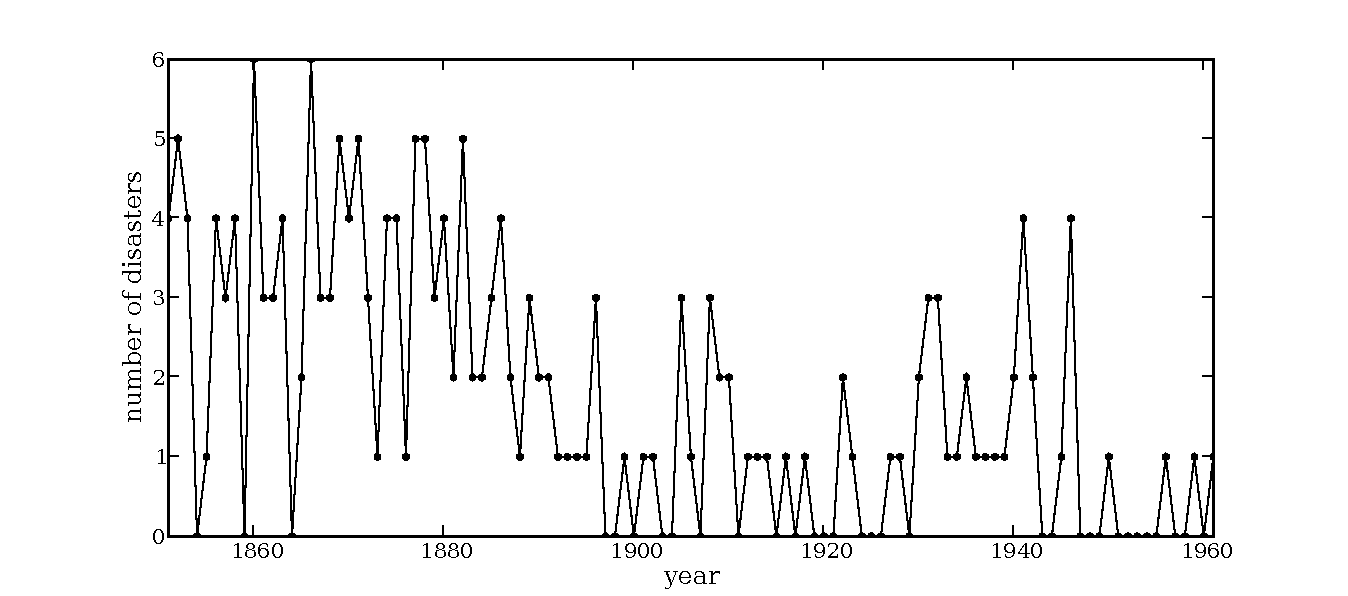
\epsfig{file=disaster_ts.pdf, width=15cm}
\end{center}
Occurrences of disasters in the time series is thought to be derived from a Poisson process with a large rate stoch in the early part of the time series, and from one with a smaller rate in the later part. We are interested in locating the change point in the series, which perhaps is related to changes in mining safety regulations.

We represent our conceptual model formally as a statistical model:
\begin{eqnarray*}
(D_t | s, e, l) \sim \textup{Po}\left(r_t\right), & r_t=\left\{\begin{array}{ll}
    e & t\le s\\ l & t>s
    \end{array}\right.,&t\in[1851,1962]\\
s\sim \textup{U}(1851, 1962)\\
e\sim \textup{Exp}(1)\\
l\sim \textup{Exp}(1)
\end{eqnarray*}
The symbols have the following meanings:
\begin{description}
    \item[$D_t$:] The number of disasters in year $t$.
    \item[$r_t$:] The rate of the Poisson distribution of disasters in year $t$.
    \item[$s$:] The year in which the rate changes.
    \item[$e$:] The rate before the switchpoint $s$.
    \item[$l$:] The rate after the switchpoint.
\end{description}

The product
\begin{eqnarray*}
\prod_t p(D_t|s,e,l) p(s)p(e)p(l)
\end{eqnarray*}
gives the joint distribution $p(D,s,e,l)$ of the data and unknown stochs. This is proportional to the posterior distribution $p(s,e,l|D)$ (where $D$ collects $D_t$ for $t$ from 1851 to 1962).

In the term $p(D_t|s,e,l)$, $D_t$ is called the \emph{consequent} and $s$, $e$ and $l$ are called the \emph{antecedents}. The antecedents are sometimes called the \emph{parents} of a consequent, and the set of variables that claim a particular variable as a parent are called that variables \emph{children}. This terminology is used in PyMC.

The dependence structure of a statistical model can be represented by a \emph{directed acyclic graph}. For our coal-mining disaster model, the PyMC-generated DAG is illustrated in figure \ref{fig:disaster_dag}. The arrows in the figure point from parent to child, or alternatively from antecedent to consequent.

\begin{figure}[hhhhhhhhhhh]
\begin{center}
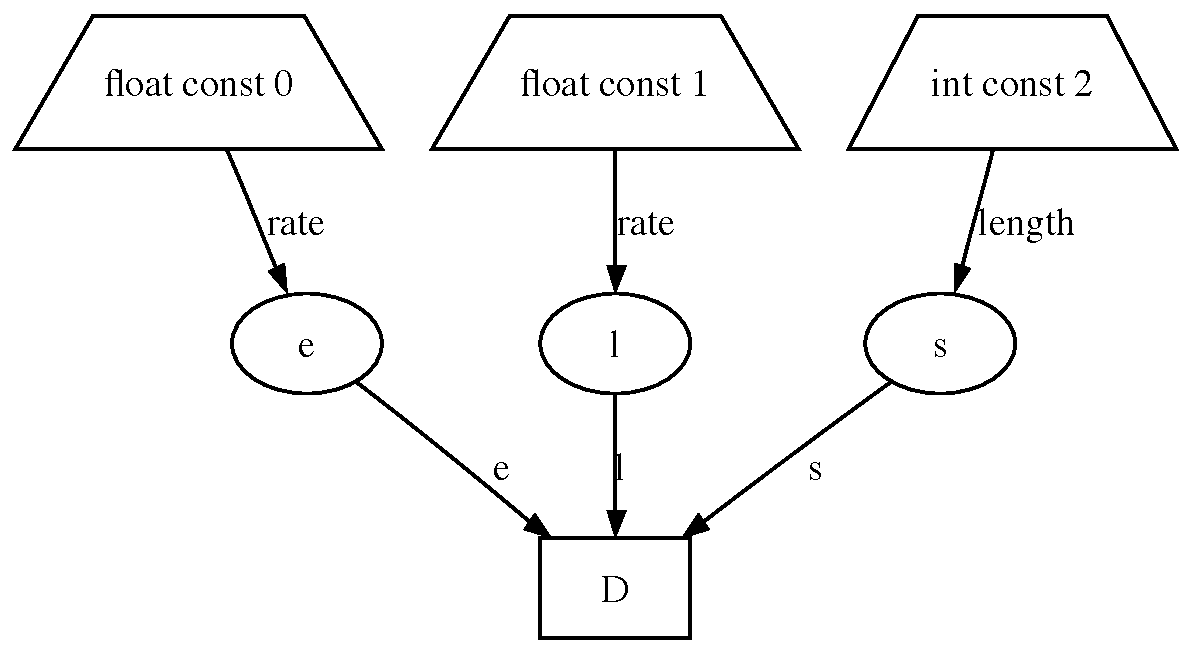
\epsfig{file=DisasterModel.pdf,width=7cm}
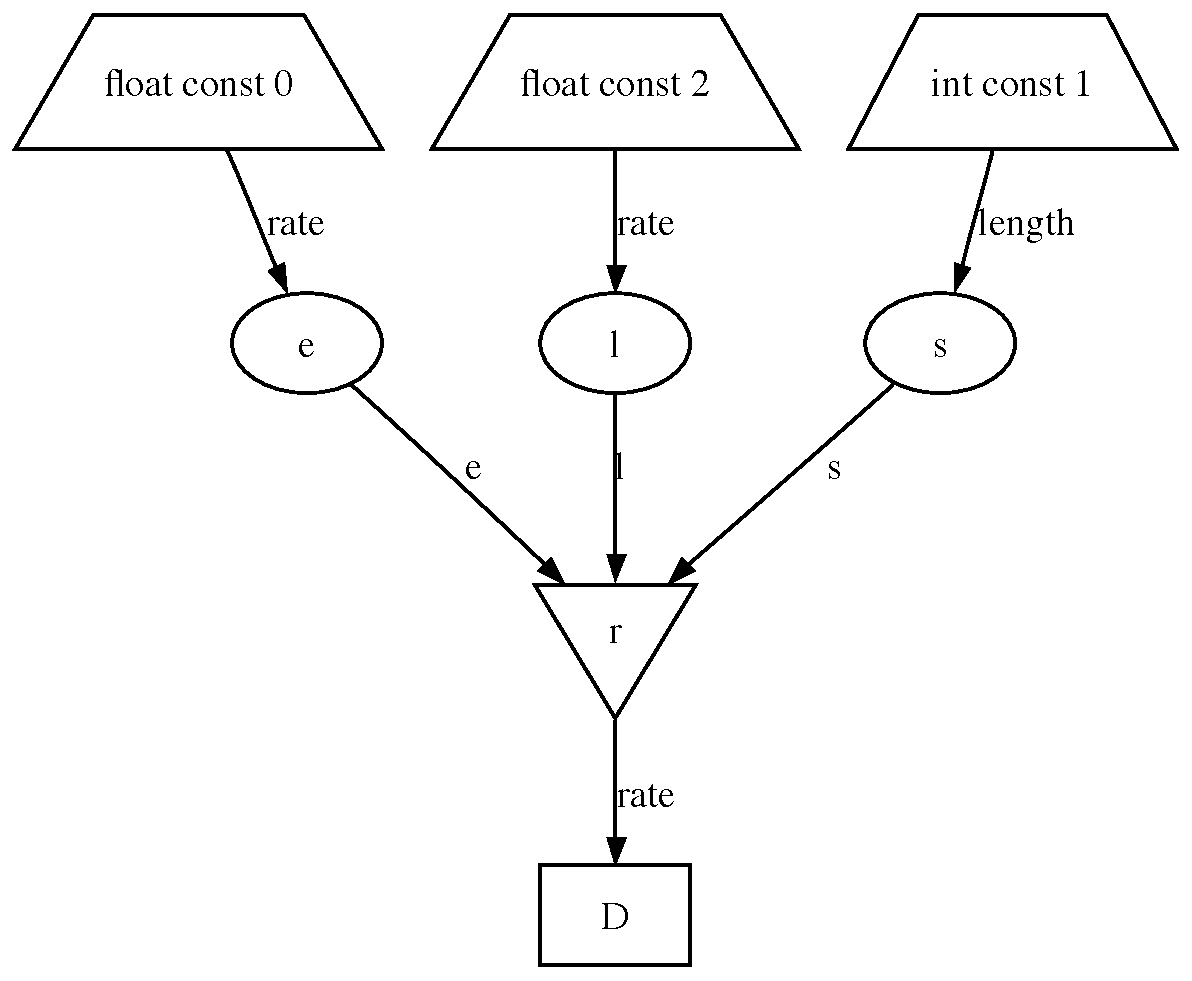
\epsfig{file=DisasterModel2.pdf,width=7cm}
\caption{\textbf{Left:} A DAG of the coal-mining disaster example with the function $r_t$ implicit. \textbf{Right:} An equivalent DAG with $r_t$ explicit. The `float const's refer to the stochs of the priors of $e$, $l$ and $s$. The labels on the arrows refer to the 	\code{Stochastic} names assigned to the parents by the child. For example, in the DAG on the right $D$ considers $r$ to be its `rate' stoch.
}
\label{fig:disaster_dag}
\end{center}
\end{figure}

In principle, we could have written down other statistical models that gave the same joint distribution (and hence the same posterior distribution). For example, we could have specified the model as
\begin{eqnarray*}
p(s|D,l,e)\prod_tp(D_t|l,e,D_{1851\ldots t-1})p(l)p(e),
\end{eqnarray*}
and drawn a new DAG representation of the dependence structure. However, that would have been extremely uncomfortable. Our intuition tells us that $e$, $l$ and $s$ influence $D_t$, not that $D_t$, $e$ and $l$ influence $s$. In other words, the statement
\begin{quote}
Given the rate before the switchpoint, the rate after the switchpoint, and the switchpoint itself, the distribution of disasters in year $t$ is $d$.
\end{quote}
is much more natural than the statement
\begin{quote}
Given the rate befare the switchpoint, the rate after the switchpoint, and annual disasters up to year $t-1$, the distribution of disasters in year $t$ is $d^*$. Further, given all the data on annual disasters the distribution of the switchpoint is $d^{**}$.
\end{quote}

Bayesian methods, and statistics in general, are usually needed \emph{because} it's natural to think of the data as consequences of the inferential targets. This point can be counterintuitive at first, as most scientists' instinct is to regard data as fixed a priori and unknown stochs' values as dependent on the data. However, it's important to understand for effective model-building in PyMC.



\section{\code{Stochastic} and \code{Deterministic}}\label{sec:PyMCObjects}
PyMC provides two built-in types to serve as the building blocks of Bayesian probability models in Python. A \code{Stochastic} object represents a variable whose distribution depends on its parents, but which is not completely determined by its parents. This is sometimes referred to as a random variable, though it need not be random in the frequentist sense. In the coal-mining disaster model, $s$, $l$, $e$ and $D$ are all stochs, but $r$ is not. Since the value of $D$ has been observed, its \code{isdata} flag would be set to true; see section \ref{sub:@data}. A dtrm object, on the other hand, represents a variable that is completely determined by its parents. In the coal-mining disaster model, $r$ is a dtrm.

These objects are meant to do only what their mathematical counterparts `do,' and to do it efficiently. As such, they have very limited awareness of the probability model in which they are embedded and no methods for updating their values in an MCMC loop given the rest of the model. PyMC leaves \code{Stochastic} updating dtrmity to the \code{StepMethod} class (sec \ref{sec:StepMethod}) and model-level dtrmity to the \code{Model} class (sec \ref{sec:Model})

PyMC also provides a special container class for stochs and dtrms to ease programming of certain dependency situations, such as when a particular variable depends on every element of a Markov chain.

\subsection{\code{Stochastic}}\label{sub:stoch}

\code{Stochastics} expose the following attributes:
\begin{description}
    \item[\code{parents}:] A dictionary containing self's parents. The keys of the dictionary correspond to the names assigned to self's parents by self, and the values correspond to the actual parents. For example, a normally-distributed stoch's parents would probably be keyed as \code{mu} and \code{tau}, \code{V} or \code{sigma}. Since PyMC inherits Python's weak typing, parents may be of any class or type.
    \item[\code{children}:] A set containing self's children, which must be stochs or dtrms. This set is produced automatically; the user doesn't need to worry about filling it.
    \item[\code{value}:] Self's current value, which is updated many times over the course of an MCMC loop. Attempts to update this attribute raise an error if \code{isdata} is true. Again, this may be of any class or type.
    \item[\code{isdata}:] A boolean indicating whether the self's value has been observed (is fixed).
    \item[\code{trace}:] The trace object assigned to self, see \textbf{XXX}.
    \item[\code{logp}:] The log-probability or log-density of self's current value, conditional on self's parents' current values. This attribute is automatically updated every time it is accessed. In addition, \code{Stochastic} caches its most recent log-probabilities to avoid unnecessary recomputation. See section \ref{sub:caching}.
    \item[\code{\_\_name\_\_}:] The name of the stoch, should be unique.
    \item[\code{\_\_doc\_\_}:] The docstring of the stoch.
\end{description}

\code{Stochastics} have the following methods:
\begin{description}
	\item[\code{touch()}:] PyMC stochs and dtrms cache the last few values of their arguments. If a stoch's log-probability or a dtrm's value is queried when their arguments' value configuration is in their cache, they don't recompute. This is called `memoization'. The price of this optimization is that stochs' values can't be updated in-place, or else the next recompute may be incorrectly skipped. If you update a stoch's value in-place, be sure to call this method afterward. It simply replaces the stoch's value with a shallow copy of itself.
    \item[\code{random()}:] This causes self to draw its value from its distribution conditional on its parents, and returns that value. This is useful for model averaging and certain Metropolis-Hastings algorithms. Raises an error if no \code{random} argument was passed to the constructor (ie, if the `medium' interface was used, see below).
\end{description}

\subsubsection{Instantiation}
In order to make specification of standard probability models easy while making room for specification of even the most exotic probability model, PyMC provides four ways to instantiate stochs.
\begin{description}
    \item[Short] \textbf{XXX}
    \item[Medium] A normally-distributed \code{Stochastic} called \code{A} could be instantiated using the medium interface as follows:
    \begin{verbatim}
@stoch
def A(value=3., mu=B, tau=C):
    """Stochastic A is normally distributed."""
    return 0.5 * tau * (value-mu)**2 + 0.5*log(0.5*tau/PI)
    \end{verbatim}
    The decorator \code{stoch} turns the function \code{A} into a \code{Stochastic} which evaluates its log-probability using \code{A}. The \code{value} argument, which is required, provides an initial value for the stoch. The names of the function's other arguments become the keys of the stoch's \code{parents} dictionary, which maps to the corresponding values (parent objects). The name of the function (in this case \code{A}) becomes the \code{\_\_name\_\_} of the stoch, and the docstring of the function is passed on to the \code{Stochastic} as well.

    The \code{Stochastic} may be valued as any object, its parents may be any objects, and there is absolutely no restriction on the log-probability function, as long as it returns a \code{float}. Note that, although the log-probability function is written out for illustration, it would be much faster to return \code{normal\_like(value, mu, tau)}

    The medium interface's decorator can take a flag called \code{trace} which signals to \code{Model} whether an MCMC trace should be kept for this stoch: \code{@stoch(trace = False)}.
    \item[Long] The long interface extends the medium interface by allowing the user to specify a method for sampling the stoch's value conditional only on its parents.
    \begin{verbatim}
@stoch
def A(value=3., mu=B, tau=C):
    """Stochastic A is normally distributed."""

    def logp(value, mu, tau):
        return 0.5 * tau * (value-mu)**2 + 0.5*log(0.5*tau/PI)

    def random(mu, tau):
        return rnormal(mu, tau)

    rseed = 1.
    \end{verbatim}
The \code{Stochastic} again gets its name, docstring and parents from \code{A}, but in this case it will evaluate its log-probability using the \code{logp} function. The \code{random} function is used when \code{Stochastic.random()} is called. Note that it doesn't take a \code{value} argument, because it provides a new value. \textbf{XXX} \code{rseed} provides a seed for the RNG.

    \item[Direct] Some users may prefer not to use the \code{stoch} decorator, but to instantiate \code{Stochastic} directly:
\begin{verbatim}
def A_logp(value, mu, tau):
    return 0.5 * tau * (value-mu)**2 + 0.5*log(0.5*tau/PI)

A = Stochastic(logp = A_logp, name = 'A', value = 3.,
parents = {'mu': B, 'tau': C}[,
doc = 'Stochastic A is normally distributed',
random = rnormal, trace = True, rseed = 1., isdata = False,
cache_depth = 2])
\end{verbatim}
\end{description}



\subsection{The \code{data} decorator}\label{sub:@data}
In the medium and long interfaces, the stoch's \code{isdata} flag can be set to true by replacing \code{@stoch} with \code{@data}.


\subsection{\code{Deterministic}}\label{sub:dtrm}

Deterministics expose the following attributes:
\begin{description}
    \item[\code{parents}:] A dictionary containing self's parents. The keys of the dictionary correspond to the names assigned to self's parents by self, and the values correspond to the actual parents. Since PyMC inherits Python's weak typing, parents may be of any class or type.
    \item[\code{children}:] A set containing self's children, which must be stochs or dtrms. This set is produced automatically; the user doesn't need to worry about filling it.
    \item[\code{value}:] Self's current value. Unlike stoch, self's value depends on its parents. As with stoch's \code{logp} attribute, this attribute is automatically updated every time it is accessed. Deterministics cache their last few values to avoid unnecessary recomputation. Attempts to update this attribute raise an error.
    \item[\code{trace}:] The trace object assigned to self, see \textbf{XXX}.
    \item[\code{\_\_name\_\_}:] The name of the dtrm, should be unique.
    \item[\code{\_\_doc\_\_}:] The docstring of the dtrm.
\end{description}
Deterministics have no methods.

\subsubsection{Instantiation}
Deterministics are less complicated than stochs, and PyMC provides only two ways to instantiate them:
\begin{description}
    \item[Decorator] A dtrm can be instantiated via a decorator in a way very similar to stoch's medium interface:
\begin{verbatim}
@dtrm
def D(arg_1 = E, arg_2 = F)
    """The D dtrm"""
    return sqrt(arg_1 ** 2 + arg_2 ** 2)
\end{verbatim}
The function supplied should return a new value for the dtrm (which, again, may be any object). Arguments' keys and values are converted into a parent dictionary as with stoch's medium interface. The function's \code{\_\_name\_\_} is passed on to the dtrm.
    \item[Direct] The same dtrm could be instantiated directly as follows:
\begin{verbatim}
def D_eval(arg_1, arg_2):
    return sqrt(arg_1 ** 2 + arg_2 ** 2)

D = Deterministic(eval = D_eval, name = 'D',
parents = \{'arg_1': E, 'arg_2': F\})[],
doc = 'The D dtrm',
trace = True),
cache_depth = 2]
\end{verbatim}
The \code{trace} flag signals to \code{Model} whether to keep a trace for self, as with stoch.
\end{description}
Note that dtrms have no \code{isdata} flag. If a dtrm's value were known, its parents would be restricted to the inverse image of that value under the dtrm's evaluation function. This usage case would be extremely difficult to support in generality, but it can be implemented for particular applications at the \code{StepMethod} level.

\subsection{The \code{PyMCObjectContainer} class for arrays of stochs and dtrms}\label{sub:container}
In the following hypothetical situation, it would be inconvenient to assign a unique label to each parent of $B$:
\begin{eqnarray*}
	A_0 \sim \textup N(0,V)\\
	A_{i+1}|A_i\sim\textup{N(0,V)},&i=1\ldots N\\
	B \sim \textup N\left(\sum_{i=0}^N A_i,W\right).
\end{eqnarray*}

This situation can be handled using the \code{PyMCObjectContainer} class as follows:
\begin{verbatim}
@stoch
def A(value=0., mu=0., V=V):
    """The initial value"""
    return normal_like(value, mu, V)
Alist = [A]

for i in range(1,N):
    @stoch
    def A(value=0., mu=Alist[i-1], V=V):
        """value %i""" % i
        return normal_like(value, mu, V)
    Alist.append(A)
    
A = PyMCObjectContainer(A)

@data
def B(value=0., mu=A, V=W):
    """The sum of the Markov chain"""
    return normal_like(value, sum(mu), V)   
\end{verbatim}
This works because PyMC object containers, like stochs and dtrms, expose an attribute called \code{value}. This attribute returns a copy of the (possibly nested) iterable that was passed into the container at instantiation, but with each instance of a stoch or dtrm replaced with \emph{its} value. Note that simply writing
\begin{verbatim}
@data
def B(value=0., mu=Alist, V=W):
	"""The sum of the Markov chain"""
	return normal_like(value, sum(mu), V)	
\end{verbatim}
would not have worked, because \code{list} does not expose an attribute called \code{value}. PyMC object containers can currently be constructed from any object that has a \code{\_\_getitem\_\_} method (such as lists, tuples, and numpy arrays), but not from sets.

\subsection{Examples}\label{sub:example}
Here is the coal-mining disaster model implemented in PyMC with $r$ implicit, as in the left pane of figure \ref{fig:disaster_dag}:
\begin{verbatim}
@stoch
def s(value=50, length=110):
    """Change time for rate stoch."""
    constrain(value, 0, length)
    return 0.

@stoch
def e(value=1., rate=1.):
    """Rate stoch of poisson distribution."""
    return exponential_like(value, rate)

@stoch
def l(value=.1, rate = 1.):
    """Rate stoch of poisson distribution."""
    return exponential_like(value, rate)

@data
def D(  value = D_array,
        switchpoint = s,
        early_mean = e,
        late_mean = l):
    """Annual occurences of coal mining disasters."""
    return poisson_like(value[:s],e) + poisson_like(value[s:],l)
\end{verbatim}
To make $r$ explicit as in the right pane of figure \ref{fig:disaster_dag}, we would write:
\begin{verbatim}
@stoch
def s(value=50, length=110):
    """Change time for rate stoch."""
    constrain(value, 0, length)
    return 0.

@stoch
def e(value=1., rate=1.):
    """Rate stoch of poisson distribution."""
    return exponential_like(value, rate)

@stoch
def l(value=.1, rate = 1.):
    """Rate stoch of poisson distribution."""
    return exponential_like(value, rate)

@dtrm
def r(l=l,e=e,s=s):
    """r = function(l,e,s)"""
    ret_val =  ones(111,dtype=float)
    ret_val[:s] = e
    ret_val[s:] = l
    return ret_val

@data
def D(  value = D_array, rate=r):
    """Annual occurences of coal mining D."""
    return poisson_like(value,rate)
\end{verbatim}
In general, it's better to make heavyweight functions into their own dtrms, because dtrms' caches avoid unnecessary recomputation. In this case, however, the version with $r$ implicit is quite a bit faster.

\section{The \code{Model} class} \label{sec:Model} 
This class serves as a container for probability models and as a stem class for other `model-level' classes like \code{Sampler}. Methods implemented:
\begin{description}
	\item[\code{sample\_model\_likelihood()}:] Returns an estimate of $\log p(d|M)$, the unconditional log-probability or log-density of all the data objects in model $M$. This is called by the function \code{weight()}, which finds the posterior probabilities of a set of models.
	\item[\code{DAG()}:] Outputs a graphical representation of the model.
	\item[\code{tally()}:] Tells all stochs and dtrms to record their current values in their traces.
	\item[\code{remember()}:] Tells all stochs and dtrms to set their values to a certain element of their traces.
	\item[\code{save\_state()}:] Under construction.
	\item[\code{save\_traces()}:] Under construction.
	\item[\code{seed()}:] All stochs with an \code{rseed} value draw a new value from their distributions.
\end{description}

Useful attributes:
\begin{description}
	\item[\code{containers}:] A set of self's PyMC object containers.
	\item[\code{stochs}:] A set of self's stochs.
	\item[\code{dtrms}:] A set of self's dtrms.
	\item[\code{data}:] A set of self's data objects.
\end{description}

\chapter{Model fitting with PyMC} %(fold)
\label{chap:MCMC}

%MCMC methods are algorithms that sample from probability distributions (\emph{i.e.} Monte Carlo simulation) to yield Markov chains.

\section{Monte Carlo Methods in Bayesian Analysis}

Bayesian model specification often results in posterior forms that are difficult to manipulate analytically. Expand- when data are children of other stochs, it's not natural to simulate directly. However, it is often possible to generate simulated values that share the distributional properties of the specified posterior. Such simulations may be summarized in such a way that describes the posterior density. For example, consider the expected value of some integral quantity:

\[
E[{\bf x}] = \int_{-\infty}^{\infty} {\bf x} f({\bf x}) d{\bf x}, \qquad
{\bf x} = \{x_1,...,x_k\}
\]

\noindent where $k$ is perhaps very large, making the joint distribution of ${\bf x}$ analytically complex. If we can produce random vectors $\{{\bf x_i}\}$, we can use these values to approximate the unknown integral. This process is known as {\emph Monte Carlo integration}. In general, MC integration says that:

\[
I[a,b] = \int_a^b h(x) f(x) dx
\]

\noindent can be estimated by:

\[
\hat{I}[a,b] = \frac{1}{n}\sum_{i=1}^n h(x_i)
\]

\noindent This estimate is useful because:

\begin{itemize}
\item
By the strong law of large numbers:
\[\hat{I}[a,b] \rightarrow I[a,b] \mbox{with probability 1}\]
\item
Simulation error can be measured and controlled:
\[Var(\hat{I}[a,b]) = \frac{1}{n(n-1)}\sum_{i=1}^n (h(x_i)-\hat{I}[a,b])^2\]
\end{itemize}

Why is this relevant to Bayesian analysis? If we replace $f(x)$ with a posterior, $\pi(\theta|x)$ and make $h(x)$ an interesting function of the unknown stoch, the resulting expectation is that of the posterior of $h(\theta)$:

\[
E[h(\theta|x)] = \int \pi(\theta|x) h(\theta) d\theta \approx \frac{1}{n}\sum_{i=1}^n h(\theta)
\]

\subsection{Rejection Sampling}

Though Monte Carlo integration allows us to estimate integrals that are unassailable by analysis, it relies on the ability to draw samples from the posterior distribution. For known stochetric forms, this is not a problem; probability integral transforms or bivariate techniques (e.g Box-Muller method) may be used to obtain samples from uniform pseudo-random variates generated from a computer. Often, however, we cannot readily generate random values from non-standard posteriors. In such instances, we can use rejection sampling to generate samples.

\begin{figure}[ht]
        \begin{center}
        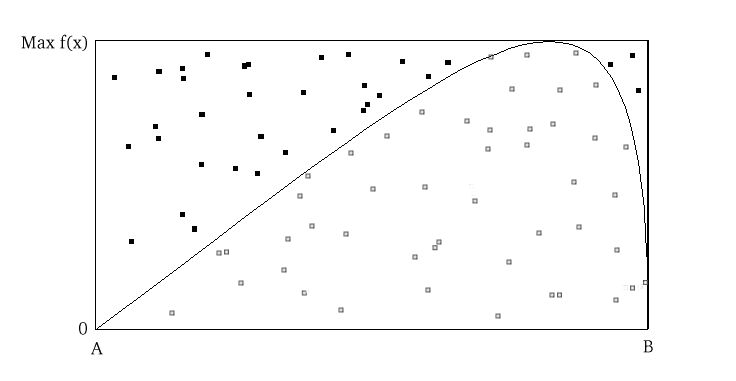
\includegraphics[scale=0.4]{reject.png}
    \end{center}
    \caption{Rejection sampling of a bounded form. Area is estimated by the ratio of accepted (open squares) to total points, multiplied by the rectangle area.}
    \label{fig:bound}
\end{figure}

Posit a function, $f(x)$ which can be evaluated for any value on the support of $x:S_x = [A,B]$, but may not be integrable or easily sampled from. If we can calculate the maximum  value of $f(x)$, we can then define a rectangle that is guaranteed to contain all possible values $(x,f(x))$. It is then trivial to generate points over the box and enumerate the values that fall under the curve (Figure \ref{fig:bound}).

\[
\frac{\mbox{Points under curve}}{\mbox{Points generated}} \times \mbox{box area} = \lim_{n \to \infty} \int_A^B f(x) dx
\]

\begin{figure}[h]
        \begin{center}
        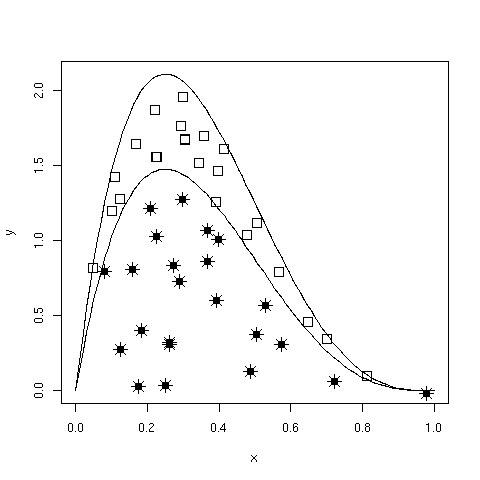
\includegraphics[scale=0.4]{envelope.png}
    \end{center}
    \caption{Rejection sampling of an unbounded form using an enveloping distribution.}
    \label{fig:unbound}
\end{figure}

\noindent This approach is useful, for example, in estimating the normalizing constant for posterior distributions.

If $f(x)$ has unbounded support (i.e. infinite tails), such as a Gaussian distribution, a bounding box is no longer appropriate. We must specify a majorizing (or, enveloping) function, $g(x)$, which implies:

\[
g(x) \le  f(x) \qquad\forall x \in (-\infty,\infty)
\]

Having done this, we can now sample ${x_i}$ from $g(x)$ and accept or reject each of these values based upon $f(x_i)$. Specifically, for each draw $x_i$, we also draw a uniform random variate $u_i$ and accept $x_i$ if $u_i < f(x_i)/kg(x_i)$ (Figure \ref{fig:unbound}). This approach is made more efficient by choosing an enveloping distribution that is ``close'' to the target distribution, thus maximizing the number of accepted points. Further improvement is gained by using optimized algorithms such as importance sampling (see text) which, as the name implies, samples more frequently from important areas of the distribution.

\section{Markov Chains}

A Markov chain is a special type of \emph{stochastic process}. The standard definition of a stochastic process is an ordered collection of random variables:

\[
\{X_t:t \in T\}
\]

\noindent where $t$ is frequently (but not necessarily) a time index. If we think of $X_t$ as a state $X$ at time $t$, and invoke the following dependence condition on each state:

\[
Pr(X_{t+1}=x_{t+1} | X_t=x_t, X_{t-1}=x_{t-1},\ldots,X_0=x_0) = Pr(X_{t+1}=x_{t+1} | X_t=x_t)
\]

\noindent then the stochastic process is known as a Markov chain. This conditioning specifies that the future depends on the current state, but not past states. Thus, the Markov chain wanders about the state space, remembering only where it has just been in the last time step. The collection of transition probabilities is sometimes called a \emph{transition matrix} when dealing with discrete states, or more generally, a \emph{transition kernel}. In the context of Markov chain Monte Carlo, useful to think of the Markovian property as ``mild non-independence''\footnote{In general, for Bayesian analyses, statistical independence is less relevant, relative to classical statistical inference. Instead, we substitute the notion of \emph{exchangeability}, which is a weaker concept, but often just as useful. Exchangeability essentially implies that different permutations (orderings) of a sequence of random variables will have the same marginal distribution. A sequence of random quantities may not be considered independent in a Bayesian sense, but are frequently exchangeable.}. We will see that, while it may be difficult to generate independent samples from a particular posterior distribution, it may be possible to generate dependent samples that may be useful in describing that distribution.

\subsection{Jargon-busting}

Before we move on, it is important to define some general properties of Markov chains. They are frequently encountered in the MCMC literature, and some will help us decide whether MCMC is producing a useful sample from the posterior.

\begin{itemize}
\item \emph{Homogeneity}: A Markov chain is homogeneous at step $t$ if the transition probabilities are independent of the state at $t$. The starting point of the chain is almost never homogeneous, as the initial values are either hand-picked or arbitrary.
\item \emph{Irreducibility}: A Markov chain is irreducible if every state is accessible in one or more steps from any other state. That is, the chain contains no absorbing states. This implies that there is a non-zero probability of eventually reaching state $k$ from any other state in the chain.
\item \emph{Recurrence}: States which are visited repeatedly are \emph{recurrent}. If the expected time to return to a particular state is bounded, this is known as \emph{positive recurrence}, otherwise the recurrent state is \emph{null recurrent}. Further, a chain is \emph{Harris recurrent} when it visits all states $X \in S$ infinitely often in the limit as $t \to \infty$; this is an important characteristic when dealing with unbounded, continuous state spaces. Whenever a chain ends up in a closed, irreducible set of Harris recurrent states, it stays there forever and visits every state with probability one.
\item \emph{Stationarity}: A stationary Markov chain produces the same marginal distribution when multiplied by the transition kernel.  Thus, if $P$ is some $n \times n$ transition matrix:

\[{\bf \pi P} = {\bf \pi}\]

\noindent for Markov chain $\pi$. Thus, $\pi$ is no longer subscripted, and is referred to as the \emph{limiting distribution} of the chain. In MCMC, the chain explores the state space according to its limiting marginal distribution.
\item \emph{Ergodicity}: Ergodicity is an emergent property of Markov chains which are irreducible, positive Harris recurrent and aperiodic. Ergodicity is defined as:

\[
\lim_{n \to \infty} Pr^{(n)}(\theta_i,\theta_j) = \pi(\theta_j) \quad \forall \theta_i, \theta_j \in \Theta
\]

\noindent or in words, the marginal distribution of the chain is the same at one step as at all other steps. This implies that our Markov chain, which we recall is dependent, now generates quantities that are independent. If it means anything to you, ergodicity is the analogue of the strong law of large numbers for Markov chains. For example, take values $\theta_{i+1},\ldots,\theta_{i+n}$ from a chain that has reached an ergodic state. A statistic of interest can then be estimated by:

\[
\hat{h}(\theta) = \frac{1}{n}\sum_{j=i+1}^{i+n} h(\theta_j) \approx h(\theta)
\]

\end{itemize}

\section{Why MCMC Works: Reversible Markov Chains}

Markov chain Monte Carlo simulates a Markov chain for which some function of interest (\emph{e.g.} the joint distribution of the stochs of some model) is the unique, invariant limiting distribution. An invariant distribution with respect to some Markov chain with transition kernel $Pr(y \mid x)$ implies that:
\[
\int_x Pr(y \mid x) \pi(x) dx = \pi(y),
\]
and similarly:
\[
\int_y Pr(x \mid y) \pi(y) dy = \pi(x),
\]

Invariance is guaranteed for any \textbf{reversible} Markov chain. Consider a Markov chain in reverse sequence: $\{\theta^{(n)},\theta^{(n-1)},...,\theta^{(0)}\}$. This sequence is still Markovian, because:
\[
Pr(\theta^{(k)}=y \mid \theta^{(k+1)}=x,\theta^{(k+2)}=x_1,\ldots ) = Pr(\theta^{(k)}=y \mid \theta^{(k+1)}=x)
\]
Forward and reverse transition probabilities may be related through Bayes theorem:
\begin{eqnarray}
Pr(\theta^{(k)}=y \mid \theta^{(k+1)}=x) &=& \frac{Pr(\theta^{(k+1)}=x \mid \theta^{(k)}=y) Pr(\theta^{(k)}=y)}{Pr(\theta^{(k+1)}=x)} \nonumber \\
&=& \frac{Pr(\theta^{(k+1)}=x \mid \theta^{(k)}=y) \pi^{(k)}(y)}{\pi^{(k+1)}(x)} \nonumber
\end{eqnarray}

\[
\frac{Pr(\theta^{(k+1)}=x \mid \theta^{(k)}=y) \pi^{(k)}(y)}{\pi^{(k+1)}(x)}
\]

\noindent Though not homogeneous in general, $\pi$ becomes homogeneous if:
\begin{itemize}
\item $n \rightarrow \infty$
\item $\pi^{(0)}=\pi$ for some $i < k$
\end{itemize}

\noindent If this chain is homogeneous it is called reversible, because it satisfies the \textbf{detailed balance equation}:
\[
\pi(x)Pr(y \mid x) = \pi(y) Pr(x \mid y)
\]
Reversibility is important because it has the effect of balancing movement through the entire state space. When a Markov chain is reversible, $\pi$ is the unique, invariant, stationary distribution of that chain.
Hence, if $\pi$ is of interest, we need only find the reversible Markov chain for which $\pi$ is the limiting distribution. This is what MCMC does!


\section{Gibbs Sampling}

The Gibbs sampler is the simplest and most prevalent MCMC algorithm. It uses samples from conditionally independent distributions to generate a sample from the fully conditional Bayesian posterior. For example, if a posterior has $k$ stochs to be estimated, we may condition each stoch on current values of the other $k-1$ stochs, and sample from the resultant distributional form (usually easier), and repeat this operation on the other stochs in turn. Note that we have now combined Markov chains (conditional independence) and Monte Carlo techniques (estimation by simulation) to yield Markov chain Monte Carlo.

Here is a stereotypical Gibbs sampling algorithm:

\newcounter{lcount}
\begin{list}{\arabic{lcount}}
{\usecounter{lcount}}
\item Choose starting values for states (stochs): ${\bf \theta} = [\theta_1^{(0)},\theta_2^{(0)},\ldots,\theta_k^{(0)}]$
\item Initialize counter $j=1$
\item Draw the following values from each of the $k$ conditional distributions:
\begin{eqnarray*}
\theta_1^{(j)} &\sim& \pi(\theta_1 | \theta_2^{(j-1)},\theta_3^{(j-1)},\ldots,\theta_{k-1}^{(j-1)},\theta_k^{(j-1)}) \\
\theta_2^{(j)} &\sim& \pi(\theta_2 | \theta_1^{(j)},\theta_3^{(j-1)},\ldots,\theta_{k-1}^{(j-1)},\theta_k^{(j-1)}) \\
\theta_3^{(j)} &\sim& \pi(\theta_3 | \theta_1^{(j)},\theta_2^{(j)},\ldots,\theta_{k-1}^{(j-1)},\theta_k^{(j-1)}) \\
\vdots \\
\theta_{k-1}^{(j)} &\sim& \pi(\theta_{k-1} | \theta_1^{(j)},\theta_2^{(j)},\ldots,\theta_{k-2}^{(j)},\theta_k^{(j-1)}) \\
\theta_k^{(j)} &\sim& \pi(\theta_k | \theta_1^{(j)},\theta_2^{(j)},\theta_4^{(j)},\ldots,\theta_{k-2}^{(j)},\theta_{k-1}^{(j)})
\end{eqnarray*}
\item Increment $j$ and repeat until convergence occurs.
\end{list}

As we can see from the algorithm, each distribution is conditioned on the last iteration of its chain values, constituting a Markov chain as advertised. The Gibbs sampler has all of the important properties outlined in the previous section: it is aperiodic, homogeneous and ergodic. Once the sampler converges, all subsequent samples are from the target distribution. This convergence occurs at a geometric rate.

Implementing a simple Gibbs sampler can be done easily in Python. Lets build a Gibbs sampler for estimating a single stoch; for example, simulating from a binomial distribution with a beta prior for $p$ (we assume $n$ is known). We just need a random number generator and a simple loop to iterate over each stoch:
\vspace{1cm}
\begin{verbatim}
# Import random number generators
from numpy import random
beta = random.beta
binomial = random.binomial

# Number of iterations
k=1000

# Prior stoch values
n=20
a=1
b=2

# Some fake data
data = [6,8,4,9,9,7,12]

# Empty arrays to store output
plist = []
ylist = []

# Here's the sampler
for i in range(k):

     # Sample from beta distribution
    p = beta(a+sum(data), len(data)*n-sum(data)+b)

    # Sample from binomial distribution
    y = binomial(n,p)

     # Append samples to lists
    plist.append(p)
    ylist.append(y)

# Calculate medians
plist.sort()
ylist.sort()
pmed = (plist[k/2]+plist[k/2+1])/2
ymed = (ylist[k/2]+ylist[k/2+1])/2

# Print results
print pmed, ymed
\end{verbatim}
\vspace{1cm}

\section{The Metropolis-Hastings Algorithm}

The key to success in applying the Gibbs sampler to the estimation of Bayesian posteriors is being able to specify the form of the complete conditionals of ${\bf \theta}$. In fact, the algorithm cannot be implemented without them. Of course, the posterior conditionals cannot always be neatly specified. The Metropolis-Hastings algorithm, which is implemented by PyMC, rather than generating values from the full set of conditionals, generates candidate state transitions from an alternate distribution, and accepts or rejects each candidate probabilistically according to a specified acceptance ratio.

Let us first consider a simple Metropolis-Hastings algorithm for a single stoch, $\theta$. If necessary, we can transform $\theta$ so that its distribution $\pi(\theta)$ has support over the real line, $\theta:S_{\theta} = (-\infty,\infty)\}$, facilitating the use of convenient random variables such as the normal. This sampling distribution will be used to produce candidate variables, and is therefore referred to as the \emph{proposal distribution}, $q_t(\theta^{\prime} | \theta)$. That is, the generated value, $\theta^{\prime}$, is a \emph{possible} next value for $\theta$ at step $t+1$. We also need to be able to calculate the probability of moving back to the original value from the candidate, or $q_t(\theta | \theta^{\prime})$. These probabilistic ingredients are used to define an \emph{acceptance ratio}:

\[
a(\theta^{\prime},\theta) = \frac{q_t(\theta^{\prime} | \theta) \pi(\theta^{\prime})}{q_t(\theta | \theta^{\prime}) \pi(\theta)}
\]

\noindent The value of $\theta^{(t+1)}$ is then determined by:

\[
\theta^{(t+1)} = \left\{\begin{array}{l@{\quad \mbox{with prob.} \quad}l}\theta^{\prime} & \min(a(\theta^{\prime},\theta),1) \\ \theta^{(t)} & 1 - \min(a(\theta^{\prime},\theta),1) \end{array}\right.
\]

\noindent This transition kernel implies that movement is not guaranteed at every step. It only occurs if the suggested transition is likely based on the acceptance ratio.

A single iteration of the Metropolis-Hastings algorithm proceeds as follows:

\newcounter{lcount2}
\begin{list}{\arabic{lcount2}}
{\usecounter{lcount2}}
\item Sample $\theta^{\prime}$ from $q(\theta^{\prime} | \theta^{(t)})$.
\item Generate a Uniform[0,1] random variate $u$.
\item If $a(\theta^{\prime},\theta) > u$ then $\theta^{(t+1)} = \theta^{\prime}$, otherwise $\theta^{(t+1)} = \theta^{(t)}$.
\end{list}

\noindent The original form of the algorithm specified by Metropolis required that $q_t(\theta^{\prime} | \theta) = q_t(\theta | \theta^{\prime})$, which reduces $a(\theta^{\prime},\theta)$ to $\pi(\theta^{\prime})/\pi(\theta)$, but this is not necessary. In either case, the state moves to high-density points in the distribution with high probability, and to low-density points with low probability. After convergence, the Metropolis-Hastings algorithm describes the full target posterior density, so all points are recurrent.

\subsection{Random-walk Metropolis-Hastings}

A practical implementation of the Metropolis-Hastings algorithm makes use of a random-walk proposal. Recall that a random walk is a Markov chain that evolves according to:

\begin{eqnarray*}
\theta^{(t+1)} &=& \theta^{(t)} + \epsilon_t \\
\epsilon_t &\sim& f(\phi)
\end{eqnarray*}

As applied to the MCMC sampling, the random walk is used as a proposal distribution, whereby dependent proposals are generated according to:

\[
q(\theta^{\prime} | \theta^{(t)}) = f(\theta^{\prime} - \theta^{(t)}) = \theta^{(t)} + \epsilon_t
\]

Generally, the density generating $\epsilon_t$ is symmetric about zero, resulting in a symmetric chain. Chain symmetry implies that $q(\theta^{\prime} | \theta^{(t)}) = q(\theta^{(t)} | \theta^{\prime})$, which reduces the Metropolis-Hastings acceptance ratio to:

\[
a(\theta^{\prime},\theta) = \frac{\pi(\theta^{\prime})}{\pi(\theta)}
\]

The choice of the random walk distribution for $\epsilon_t$ is frequently a normal or Student's $t$ density, but it may be any distribution that generates an irreducible proposal chain.

An important consideration is the specification of the scale stoch for the random walk error distribution. Large values produce random walk steps that are highly exploratory, but tend to produce proposal values in the tails of the target distribution, potentially resulting in very small acceptance rates. Conversely, small values tend to be accepted more frequently, since they tend to produce proposals close to the current stoch value, but may result in chains that mix very slowly. Some simulation studies suggest optimal acceptance rates in the range of 20-50\%. It is often worthwhile to optimize the proposal variance by iteratively adjusting its value, according to observed acceptance rates early in the MCMC simulation.

\section{MCMC Simulation Output}

Stochastic simulation using any MCMC algorithm generates a set of $n$ samples for each stoch in the joint target distribution, where $n$ is the number of MCMC iterations chosen by the user. This sample is used for inference on the stochs of interest, by calculating sample statistics (\emph{e.g.}, mean, mode, variance, quantiles, credible intervals).

\begin{figure}[ht]
        \begin{center}
        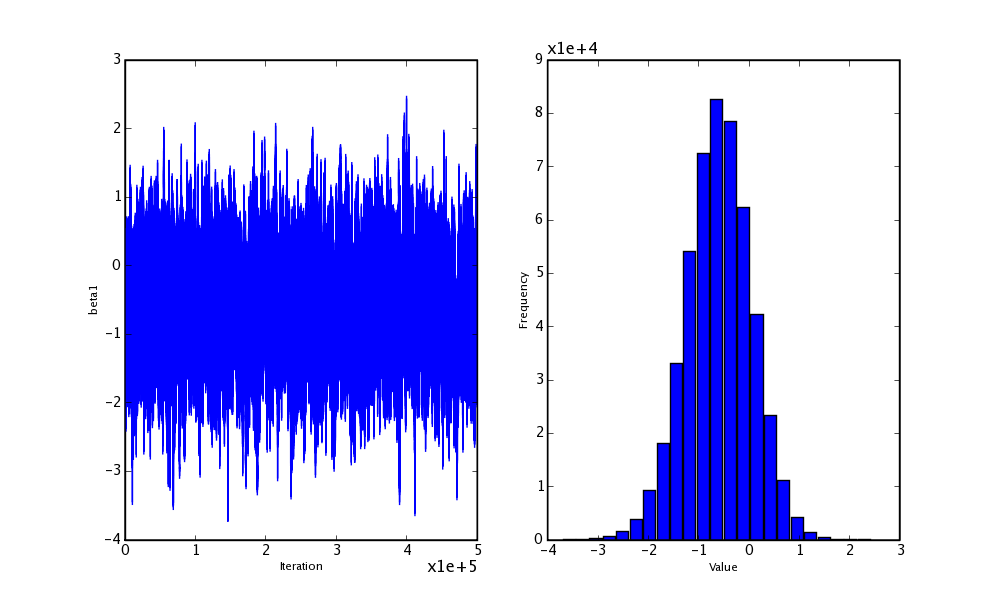
\includegraphics[scale=0.4]{sample_output.png}
    \end{center}
    \caption{Sample trace (left) and histogram (right) from Metropolis-Hastings simulation using PyMC.}
    \label{fig:sample_output}
\end{figure}

Valid inference relies on the assumption that sample values are random (but not necessarily independent) draws from the limiting distribution of the Markov chain. Typically, since unknown stochs are initialized arbitrarily, it is unlikely that the entire sample satisfies this assumption. It is usual, therefore, to discard the first portion of the sample, up to some specified proportion. The appropriate size of this ``burn-in" period is usually determined  \emph{a priori}, sometimes with the assistance of a variety of convergence diagnostics (discussed later). The number of iterations required for convergence varies strongly with the nature of the target posterior distribution and the efficiency of the chosen MCMC algorithm.

Since the sample is derived from a Markov chain, it is necessarily autocorrelated. Poorly-mixing simulations will exhibit autocorrelation more acutely, as successive samples will be relatively close (in stoch space) to their predecessors. Therefore, it is often desirable to ``thin" the sample output, by retaining every $k$ sample from the chain, where $k$ is determined by the severity of the autocorrelation function.


\section{The \code{StepMethod} class}\label{sec:StepMethod}
Sampling methods are responsible for making stochs or groups of stochs take single MCMC steps. PyMC provides several standard step methods, including \code{OneAtATimeMetropolis}, but \code{StepMethod} is designed to be subclassed to handle particular types of probability submodels. When writing your own step methods, try to make them embeddable; that is, try to make them work reliably regardless of what the probability model looks like outside of the submodel over which they have jurisdiction. If you do this, you'll accumulate a library of step methods that can be easily stuck together to fit new probability models, and you won't have to keep rewriting them.

\begin{figure}[hhhhhhhhh]
    \centering
    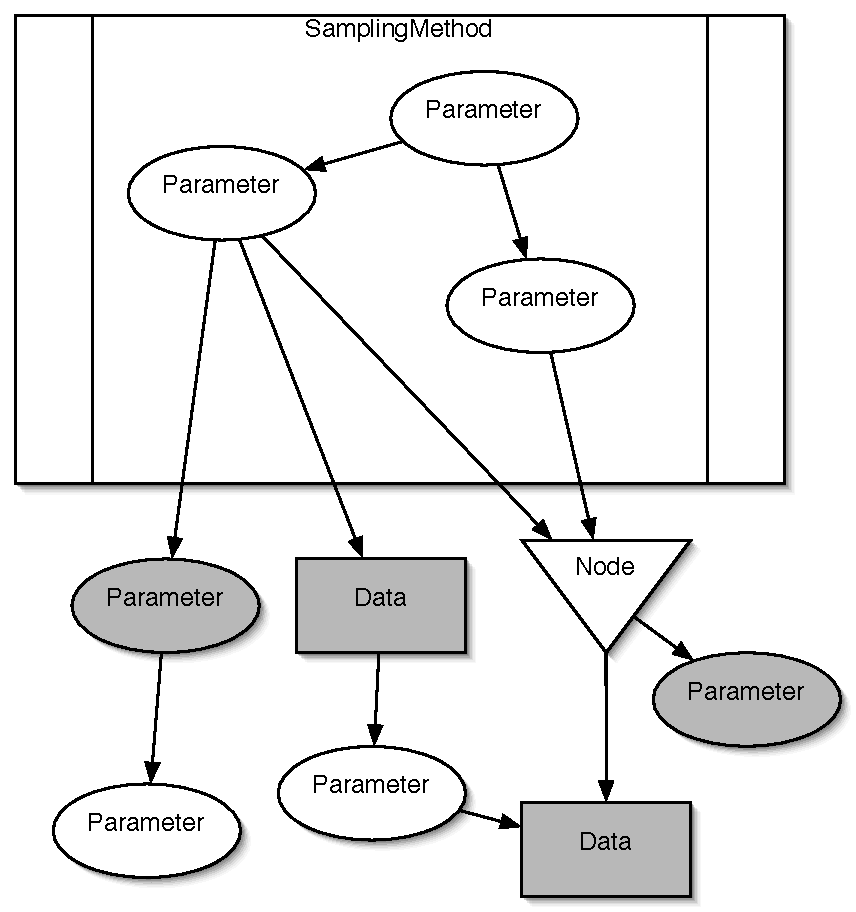
\epsfig{file=sampmethod_children.pdf,width=6cm}
    \caption{The children of a step method. The stochs under the step method's jurisdiction are shown on a plate. The children of the step method are the stochs (regardless of \code{isdata}) which depend on the step method's stochs either directly or via an unbroken sequence of dtrms, and which aren't in the step method's stochs.}
    \label{fig:sampmethod_children}
\end{figure}

All step methods must be subclasses of \code{StepMethod}, which exposes the following attributes:
\begin{description}
    \item[\code{dtrms}:] A set containing the dtrms over which self has jurisdiction. Although step methods are primarily responsible for making stochs take Metropolis steps, it can be nice to assign dtrms to them for organizational reasons.
    \item[\code{stochs}:] A set containing the stochs over which self has jurisdiction, with \code{isdata} set to false. Self will be responsible for making all of these stochs take single MCMC steps.
    \item[\code{data}:] A set containing the stochs over which self has jurisdiction, with \code{isdata} set to true. Again, this attribute is provided for the sake of organization.
    \item[\code{pymc\_objects}:] The union of \code{dtrms}, \code{stochs}, and \code{data}.
    \item[\code{children}:] The union of all the nearest descendants of self's stochs that are themselves stochs, differenced with the set of self's stochs. See figure \ref{fig:sampmethod_children}.
    \item[\code{loglike}:] The log-probability of self's children given self's stochs' current values. The sum of self's stochs' \code{logp} attributes plus \code{self.loglike}  gives the total log joint probability of self's stochs, up to superfluous constants. This attribute will be needed by most embeddable step methods. Loglike is recomputed every time it's accessed.
    \item[\code{\_asf}]: A catchall name for tunable sampling stochs.
\end{description}

\code{StepMethod} has the following methods, which aren't implemented in the base class:
\begin{description}
    \item[\code{sample()}:] \code{Model} will call this method for each step method. When it is called, self must cause each of its stochs to take an MCMC step. All subclasses must implement this method.
    \item[\code{tune()}:] \code{Model} will also call this method for each step method, but implementation is optional. When it is called, self should tune its stepping strategy somehow, possibly by adjusting \code{\_asf}.
\end{description}


\subsection{\code{OneAtATimeMetropolis}}\label{sub:OAATM}
This is PyMC's basic step method. If \code{Model}, on instantiation, finds that a stoch is not handled by any step method, it will create an instance of \code{OneAtATimeMetropolis} to handle that stoch. The easiest way to explain this simple object is just to display its source code: \textbf{XXX replace when tune() and more \_dist's are implemented}
\begin{verbatim}
class OneAtATimeMetropolis(StepMethod):

    def __init__(self, stoch, scale=1, dist='Normal'):
        StepMethod.__init__(self,[stoch])
        self.stoch = stoch
        self.proposal_sig = ones(shape(self.stoch.value)) * \
                            abs(self.stoch.value) * scale
        self.proposal_deviate = zeros(shape(self.stoch.value),dtype=float)
        self._dist = dist

    def step(self):

        # Probability and likelihood for stoch's current value:

        logp = self.stoch.logp
        loglike = self.loglike

        # Sample a candidate value
        self.propose()

        # Probability and likelihood for stoch's proposed value:
        try:
            logp_p = self.stoch.logp

        # Reject jumps to illegal values
        except LikelihoodError:
            self.stoch.revert()
            self._rejected += 1
            return

        loglike_p = self.loglike

        # Test
        if log(random()) > logp_p + loglike_p - logp - loglike:
            # Revert stoch (reject) if fail
            self.stoch.revert()

            self._rejected += 1
        else:
            # Do nothing (accept) if pass
            self._accepted += 1

    def propose(self):

        if self._dist == 'RoundedNormal':
            self.stoch.value = round(rnormal(self.stoch.value,self.proposal_sig))
        # Default to normal random-walk proposal
        else:
            self.stoch.value = rnormal(self.stoch.value,self.proposal_sig)

    def tune(self):
        #
        # Adjust _asf according to some heuristic
        #
        pass
\end{verbatim}

Note that a proposal is made by actually updating the stoch's value, and jumps are rejected by calling the stoch's \code{revert()} method. This procedure lets stochs and dtrms make the best use of their internal caches and minimizes the computation that needs to be done. Note also that, by convention, log-probability evaluation functions raise a \code{LikelihoodError} rather than returning \code{-inf} when the probability or density of a value is zero. This is done for compatibility with fortran 77, which does not recognize \code{inf}s. The function \code{random()}, from numpy, returns a random number uniformly distributed between 0 and 1.


\subsection{Other step methods provided with the distribution}\label{sub:other_sm}
\textbf{XXX} JointMetropolis, OpenCapture, ClosedCapture, whatever else.



%(end)

\section{The \code{Sampler} class}\label{sec:Sampler}
The Sampler class is a subclass of Model. In addition to those inherited from Model, it has the following attributes:
\begin{description}
	\item[\code{sampling\_methods}:]
\end{description}
and the following methods:
\begin{description}
	\item[\code{tune()}:]
	\item[\code{sample()}:]
	\item[\code{interactive\_sample()}:] 
\end{description}


\chapter{Diagnostics} %(fold)

\section{Convergence Diagnostics}

Valid inferences from sequences of MCMC samples are based on the assumption that the samples are derived from the true posterior distribution of interest. Theory guarantees this condition as the number of iterations approaches infinity. It is important, therefore, to determine the minimum number of samples required to ensure a reasonable approximation to the target posterior density. Unfortunately, no universal threshold exists across all problems, so convergence must be assessed independently each time MCMC estimation is performed. The procedures for verifying convergence are collectively known as convergence diagnostics.

One approach to analyzing convergence is analytical, whereby the variance of the sample at different sections of the chain are compared to that of the limiting distribution. These methods use distance metrics to analyze convergence, or place theoretical bounds on the sample variance, and though they are promising, they are generally difficult to use and are not prominent in the MCMC literature. More common is a statistical approach to assessing convergence. With this approach, rather than considering the properties of the theoretical target distribution, only the statistical properties of the observed chain are analyzed. Reliance on the sample alone restricts such convergence criteria to heuristics; that is, convergence cannot be guaranteed. Although evidence for lack of convergence using statistical convergence diagnostics will correctly imply lack of convergence in the chain, the absence of such evidence will not \emph{guarantee} convergence in the chain. Nevertheless, negative results for one or more criteria will provide some measure of assurance to most users that their sample will provide valid inferences.

For most simple models, convergence will occur quickly, sometimes within a the first several hundred iterations, after which all remaining samples of the chain may be used to calculate posterior quantities. For many more complex models, convergence requires a significantly longer burn-in period; sometimes  orders of magnitude more samples are needed. Frequently, lack of convergence will be caused by poor mixing (Figure \ref{fig:mix}). Recall that \emph{mixing} refers to the degree to which the Markov chain explores the support of the posterior distribution. Poor mixing may stem from inappropriate proposals (if one is using the Metropolis-Hastings sampler) or from attempting to estimate models with highly correlated stochs.

\begin{figure}[ht]
\begin{center}
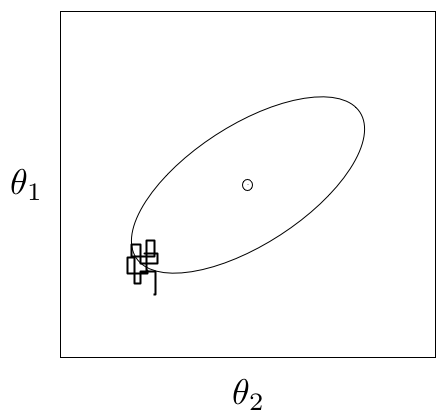
\includegraphics[height=3in]{poor_mixing.png}
\caption{An example of a poorly-mixing sample in two dimensions. Notice that the chain is trapped in a region of low probability relative to the mean (dot) and variance (oval) of the true posterior quantity.}
\label{fig:mix}
\end{center}
\end{figure}

\section*{Informal Methods}

The most straightforward approach for assessing convergence is based on simply plotting and inspecting traces and histograms of the observed MCMC sample. If the trace of values for each of the stochs exhibits asymptotic behaviour\footnote{Asymptotic behaviour implies that the variance and the mean value of the sample stays relatively constant over some arbitrary period.} over the last $m$ iterations, this may be satisfactory evidence for convergence. A similar approach involves plotting a histogram for every set of $k$ iterations (perhaps 50-100) beyond some burn in threshold $n$; if the histograms are not visibly different among the sample intervals, this is reasonable evidence for convergence. Note that such diagnostics should be carried out for each stoch estimated by the MCMC algorithm, because convergent behaviour by one stoch does not imply evidence for convergence for other stochs in the analysis. An extension of this approach can me taken when multiple parallel chains are run, rather than just a single, long chain. In this case, the final values of $c$ chains run for $n$ iterations are plotted in a histogram; just as above, this is repeated every $k$ iterations thereafter, and the histograms of the endpoints are plotted again and compared to the previous histogram. This is repeated until consecutive histograms are indistinguishable.

\begin{figure}[h]
\begin{center}
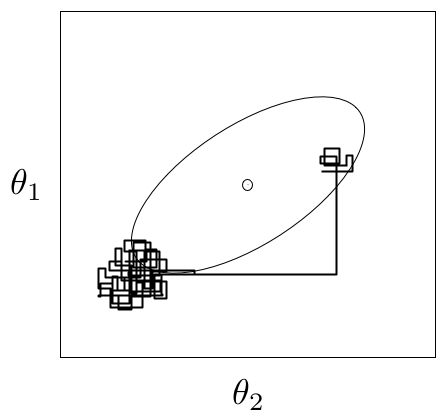
\includegraphics[height=3in]{metastable.png}
\caption{An example of metastability in a two-dimensional stoch space. The chain appears to be stable in one region of the stoch space for an extended period, then unpredictably jumps to another region of the space.}
\label{fig:metas}
\end{center}
\end{figure}

Another \emph{ad hoc} method for detecting convergence is to examine the traces of several MCMC chains initialized with different starting values. Overlaying these traces on the same set of axes should (if convergence has occurred) show each chain tending toward the same equilibrium value, with approximately the same variance. Recall that the tendency for some Markov chains to converge to the true (unknown) value from diverse initial values is called \emph{ergodicity}. This property is guaranteed by the reversible chains constructed using MCMC, and should be observable using this technique. Again, however, this approach is only a heuristic method, and cannot always detect lack of convergence, even though chains may appear ergodic.

A principle reason that evidence from informal techniques cannot guarantee convergence is a phenomenon called metastability. Chains may appear to have converged to the true equilibrium value, displaying excellent qualities by any of the methods described above. However, after some period of stability around this value, the chain may suddenly move to another region of the stoch space (Figure \ref{fig:metas}). This period of metastability can sometimes be very long, and therefore escape detection by these convergence diagnostics. Unfortunately, there is no statistical technique available for detecting metastability.

\section*{Formal Methods}

Along with the \emph{ad hoc} techniques described above, a number of more formal methods exist which are prevalent in the literature. These are considered more formal because they are based on existing statistical methods, such as time series analysis.

PyMC includes one formal convergence diagnostic method, first proposed by \citet{Geweke:1992gm}. This is a time-series approach, which compares the mean and variance of segments from the beginning and end of a single chain.
\begin{equation}
z = \frac{\bar{\theta}_a - \bar{\theta}_b}{\sqrt{Var(\theta_a) + Var(\theta_b)}}
\end{equation}
where $a$ is the early interval and $b$ the late interval. If the z-scores of these two segments are similar, it can provide evidence for convergence. PyMC plots the z-scores of the difference between various initial segments along the chain, and the last 50\% of the remaining chain. If the chain has converged, the majority of points should fall within 2 standard deviations of zero. Calling the convergence method results in a diagnostic plot for each model stoch.

\subsubsection{Method Usage}
\begin{verbatim}
sampler.convergence(first=0.1, last=0.5, intervals=20, burn=0, thin=1, chain=-1, plot=True)
\end{verbatim}
\begin{itemize}

\item \verb=first= (optional): First portion of chain to be used in Geweke diagnostic. Defaults to 0.1 (i.e. first 10% of chain).

\item \verb=last= (optional): Last portion of chain to be used in Geweke diagnostic. Defaults to 0.5 (i.e. last 50% of chain).

\item \verb=intervals= (optional): Number of sub-chains to analyze. Defaults to 20.

\item \verb=burn (optional)=: Number of burn-in iterations to exclude. Defaults to 0 (\emph{i.e.} no burn-in).

\item \verb=thin (optional)=: Thinning factor. Defaults to 1 (\emph{i.e.} no thinning).

\item \verb=chain= (optional): Chain to be analyzed. Defaults to -1 (\emph{i.e}. last chain).

\item \verb=plot= (optional): Plotting flag. Defaults to True.
\end{itemize}
Comprehensive convergence diagnostics are available in the \href{http://lib.stat.cmu.edu/R/CRAN/}{R statistical package}, via the \href{http://www-fis.iarc.fr/coda/}{CODA module}. The \verb=MetropolisHastings= class in PyMC includes a method for exporting model traces in a format that may be directly read by CODA.

\subsubsection{Method Usage}
\begin{verbatim}
sampler.coda_output(filename="coda", burn=0, thin=1)
\end{verbatim}
\begin{itemize}

\item \verb=filename= (optional): Filename of coda output files. Defaults to ``coda''.

\item \verb=burn (optional)=: Number of burn-in iterations to exclude. Defaults to 0 (\emph{i.e.} no burn-in).

\item \verb=thin (optional)=: Thinning factor. Defaults to 1 (\emph{i.e.} no thinning).

\end{itemize}
Calling \verb=coda_output= yields a \verb=.out= file containing raw trace values and a \verb=.ind= file containing indices.

\section{Goodness-of-Fit}

PyMC provides a flexible method for assessing goodness-of-fit (GOF) of models following MCMC estimation. Following \citet{Gelman:1996gp}, the \verb=goodness= method from the \verb=MetropolisHastings= sampler assesses GOF using a simple discrepancy measure for each component of the likelihood. This measure compares the deviance of the data from the expected stoch values to deviance of simulated data from the expected stoch values. Data are simulated based on samples from the trace of all the stochs. These observed and simulated deviances are plotted against one another to yield GOF plots:

Evidence for lack of fit is apparent when points do not fall on either side of the diagonal in approximately the same numbers; the example above shows very good fit. One plot is generated for every component of the likelihood bearing the same name. Additionally, PyMC reports a GOF statistic (which some authors regrettably call the Bayesian $p$-value), which is simply the proportion of points where the simulated deviance is greater than the observed deviance. This value should be close to 0.5 for a well-fit model.

\subsubsection{Method Usage}
\begin{verbatim}
sampler.goodness(iterations, plot=True, loss='squared', burn=0, thin=1, chain=-1, composite=False)
\end{verbatim}

\begin{itemize}

\item \verb=iterations=: Number of GOF iterations to run.

\item \verb=plot (optional)=: Plotting flag. Defaults to True.

\item \verb=loss (optional)=: Loss function to use. Valid arguments include ‘squared’, ‘absolute’ and ‘chi-square’. Defaults to ‘squared’.

\item \verb=burn (optional)=: Number of burn-in iterations to exclude. Defaults to 0 (\emph{i.e.} no burn-in).

\item \verb=thin (optional)=: Thinning factor. Defaults to 1 (\emph{i.e.} no thinning).

\item \verb=chain (optional)=: Chain to be analyzed. Defaults to -1 (\emph{i.e.} last chain).

\item \verb=composite (optional)=: Flag for composite GOF analysis (\emph{i.e.} based on all chains combined). Defaults to False.
\end{itemize}


\subsubsection{Method Usage}
\section{Autocorrelation Plots}

Samples from MCMC algorithms are ususally autocorrelated, due partly to the inherent Markovian dependence structure. The degree of autocorrelation can be quantified using the autocorrelation function:
\begin{eqnarray*}
    \rho_k &=& \frac{\mbox{Cov}(X_t, X_{t+k})}{\sqrt{\mbox{Var}(X_t)\mbox{Var}(X_{t+k})}} \\
            &=& \frac{E[(X_t - \theta)(X_{t+k} - \theta)]}{\sqrt{E[(X_t - \theta)^2] E[(X_{t+k} - \theta)^2]}}
\end{eqnarray*}
The \verb=MetropolisHastings= class includes a method for plotting the autocorrelation function for each stoch in the sampler (Figure \ref{fig:autocorr}). This allows users to examine the relationship among successive samples within sampled chains. Significant autocorrelation suggests that chains require thinning prior to use of the posterior statistics for inference.

\begin{figure}[htbp]
        \begin{center}
        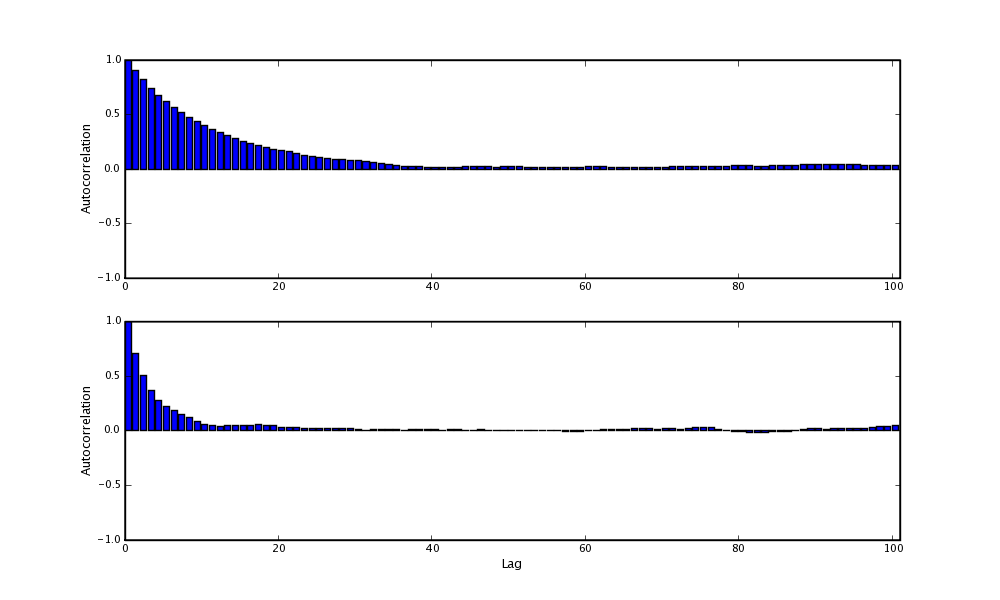
\includegraphics[scale=0.4]{autocorr.png}
    \end{center}
    \caption{Sample autocorrelation plots for two Poisson stochs from coal mining disasters example model.}
    \label{fig:autocorr}
\end{figure}

\begin{verbatim}
sampler.autocorrelation(max_lag=100, burn=0, thin=1, chain=-1)
\end{verbatim}

\begin{itemize}

\item \verb=max_lag (optional)=: Maximum time lag to calculate autocorrelation. Defaults to 100 iterations.

\item \verb=burn (optional)=: Number of burn-in iterations to exclude. Defaults to 0 (\emph{i.e.} no burn-in).

\item \verb=thin (optional)=: Thinning factor. Defaults to 1 (\emph{i.e.} no thinning).

\item \verb=chain (optional)=: Chain to be analyzed. Defaults to -1 (\emph{i.e}. last chain).
\end{itemize}

%(end)

\chapter{Advanced topics}

\section{How to make PyMC run as fast as possible}\label{sec:fast} % (fold)
\subsection{Profile your code}\label{sub:profile_your_code} % (fold)
So you can see where the bottlenecks are. It's easy in IPython. Timing your code is helpful too.

\subsection{Write fast log-probability functions}\label{sub:write_fast_log_probability_functions} % (fold)

PyMC aims to provide a fast and user-friendly interface to several standard probability distributions. However, we're not able to anticipate every usage case. We're not even going to try, but you can provide any Python-callable function you want. This is often fruitful, because in most cases the easiest way to buy efficiency is to optimize log-probability functions. Try Weave or f2py. Consider the DisasterSampler example with custom log-probability functions- speeds up by a factor of three! We've tried to keep the overhead low so optimization is worth your while. Quick runthrough of f2py.
\subsection{Optimize custom subsamplers}\label{sub:optimize_custom_subsamplers}
The second-most-likely place for a bottleneck is in a custom SubSampler. Model itself is probably not the bottleneck. Weave and f2py might be helpful here, too.

\bibliographystyle{plainnat}
\bibliography{pymc}


\appendix

\chapter{Probability distributions}
David
Link to the epydoc generated API ?
%% Generated by Sphinx.
\def\sphinxdocclass{report}
\documentclass[letterpaper,10pt,english]{sphinxmanual}
\usepackage[utf8]{inputenc}
\DeclareUnicodeCharacter{00A0}{\nobreakspace}
\usepackage[T1]{fontenc}
\usepackage{babel}
\usepackage{times}
\usepackage[Bjarne]{fncychap}
\usepackage{longtable}
\usepackage{sphinx}


\title{PyMC Documentation}
\date{August 20, 2011}
\release{2.2}
\author{Christopher J. Fonnesbeck}
\newcommand{\sphinxlogo}{}
\renewcommand{\releasename}{Release}
\makeindex

\makeatletter
\def\PYG@reset{\let\PYG@it=\relax \let\PYG@bf=\relax%
    \let\PYG@ul=\relax \let\PYG@tc=\relax%
    \let\PYG@bc=\relax \let\PYG@ff=\relax}
\def\PYG@tok#1{\csname PYG@tok@#1\endcsname}
\def\PYG@toks#1+{\ifx\relax#1\empty\else%
    \PYG@tok{#1}\expandafter\PYG@toks\fi}
\def\PYG@do#1{\PYG@bc{\PYG@tc{\PYG@ul{%
    \PYG@it{\PYG@bf{\PYG@ff{#1}}}}}}}
\def\PYG#1#2{\PYG@reset\PYG@toks#1+\relax+\PYG@do{#2}}

\def\PYG@tok@gd{\def\PYG@tc##1{\textcolor[rgb]{0.63,0.00,0.00}{##1}}}
\def\PYG@tok@gu{\let\PYG@bf=\textbf\def\PYG@tc##1{\textcolor[rgb]{0.50,0.00,0.50}{##1}}}
\def\PYG@tok@gt{\def\PYG@tc##1{\textcolor[rgb]{0.00,0.25,0.82}{##1}}}
\def\PYG@tok@gs{\let\PYG@bf=\textbf}
\def\PYG@tok@gr{\def\PYG@tc##1{\textcolor[rgb]{1.00,0.00,0.00}{##1}}}
\def\PYG@tok@cm{\let\PYG@it=\textit\def\PYG@tc##1{\textcolor[rgb]{0.25,0.50,0.56}{##1}}}
\def\PYG@tok@vg{\def\PYG@tc##1{\textcolor[rgb]{0.73,0.38,0.84}{##1}}}
\def\PYG@tok@m{\def\PYG@tc##1{\textcolor[rgb]{0.13,0.50,0.31}{##1}}}
\def\PYG@tok@mh{\def\PYG@tc##1{\textcolor[rgb]{0.13,0.50,0.31}{##1}}}
\def\PYG@tok@cs{\def\PYG@tc##1{\textcolor[rgb]{0.25,0.50,0.56}{##1}}\def\PYG@bc##1{\colorbox[rgb]{1.00,0.94,0.94}{##1}}}
\def\PYG@tok@ge{\let\PYG@it=\textit}
\def\PYG@tok@vc{\def\PYG@tc##1{\textcolor[rgb]{0.73,0.38,0.84}{##1}}}
\def\PYG@tok@il{\def\PYG@tc##1{\textcolor[rgb]{0.13,0.50,0.31}{##1}}}
\def\PYG@tok@go{\def\PYG@tc##1{\textcolor[rgb]{0.19,0.19,0.19}{##1}}}
\def\PYG@tok@cp{\def\PYG@tc##1{\textcolor[rgb]{0.00,0.44,0.13}{##1}}}
\def\PYG@tok@gi{\def\PYG@tc##1{\textcolor[rgb]{0.00,0.63,0.00}{##1}}}
\def\PYG@tok@gh{\let\PYG@bf=\textbf\def\PYG@tc##1{\textcolor[rgb]{0.00,0.00,0.50}{##1}}}
\def\PYG@tok@ni{\let\PYG@bf=\textbf\def\PYG@tc##1{\textcolor[rgb]{0.84,0.33,0.22}{##1}}}
\def\PYG@tok@nl{\let\PYG@bf=\textbf\def\PYG@tc##1{\textcolor[rgb]{0.00,0.13,0.44}{##1}}}
\def\PYG@tok@nn{\let\PYG@bf=\textbf\def\PYG@tc##1{\textcolor[rgb]{0.05,0.52,0.71}{##1}}}
\def\PYG@tok@no{\def\PYG@tc##1{\textcolor[rgb]{0.38,0.68,0.84}{##1}}}
\def\PYG@tok@na{\def\PYG@tc##1{\textcolor[rgb]{0.25,0.44,0.63}{##1}}}
\def\PYG@tok@nb{\def\PYG@tc##1{\textcolor[rgb]{0.00,0.44,0.13}{##1}}}
\def\PYG@tok@nc{\let\PYG@bf=\textbf\def\PYG@tc##1{\textcolor[rgb]{0.05,0.52,0.71}{##1}}}
\def\PYG@tok@nd{\let\PYG@bf=\textbf\def\PYG@tc##1{\textcolor[rgb]{0.33,0.33,0.33}{##1}}}
\def\PYG@tok@ne{\def\PYG@tc##1{\textcolor[rgb]{0.00,0.44,0.13}{##1}}}
\def\PYG@tok@nf{\def\PYG@tc##1{\textcolor[rgb]{0.02,0.16,0.49}{##1}}}
\def\PYG@tok@si{\let\PYG@it=\textit\def\PYG@tc##1{\textcolor[rgb]{0.44,0.63,0.82}{##1}}}
\def\PYG@tok@s2{\def\PYG@tc##1{\textcolor[rgb]{0.25,0.44,0.63}{##1}}}
\def\PYG@tok@vi{\def\PYG@tc##1{\textcolor[rgb]{0.73,0.38,0.84}{##1}}}
\def\PYG@tok@nt{\let\PYG@bf=\textbf\def\PYG@tc##1{\textcolor[rgb]{0.02,0.16,0.45}{##1}}}
\def\PYG@tok@nv{\def\PYG@tc##1{\textcolor[rgb]{0.73,0.38,0.84}{##1}}}
\def\PYG@tok@s1{\def\PYG@tc##1{\textcolor[rgb]{0.25,0.44,0.63}{##1}}}
\def\PYG@tok@gp{\let\PYG@bf=\textbf\def\PYG@tc##1{\textcolor[rgb]{0.78,0.36,0.04}{##1}}}
\def\PYG@tok@sh{\def\PYG@tc##1{\textcolor[rgb]{0.25,0.44,0.63}{##1}}}
\def\PYG@tok@ow{\let\PYG@bf=\textbf\def\PYG@tc##1{\textcolor[rgb]{0.00,0.44,0.13}{##1}}}
\def\PYG@tok@sx{\def\PYG@tc##1{\textcolor[rgb]{0.78,0.36,0.04}{##1}}}
\def\PYG@tok@bp{\def\PYG@tc##1{\textcolor[rgb]{0.00,0.44,0.13}{##1}}}
\def\PYG@tok@c1{\let\PYG@it=\textit\def\PYG@tc##1{\textcolor[rgb]{0.25,0.50,0.56}{##1}}}
\def\PYG@tok@kc{\let\PYG@bf=\textbf\def\PYG@tc##1{\textcolor[rgb]{0.00,0.44,0.13}{##1}}}
\def\PYG@tok@c{\let\PYG@it=\textit\def\PYG@tc##1{\textcolor[rgb]{0.25,0.50,0.56}{##1}}}
\def\PYG@tok@mf{\def\PYG@tc##1{\textcolor[rgb]{0.13,0.50,0.31}{##1}}}
\def\PYG@tok@err{\def\PYG@bc##1{\fcolorbox[rgb]{1.00,0.00,0.00}{1,1,1}{##1}}}
\def\PYG@tok@kd{\let\PYG@bf=\textbf\def\PYG@tc##1{\textcolor[rgb]{0.00,0.44,0.13}{##1}}}
\def\PYG@tok@ss{\def\PYG@tc##1{\textcolor[rgb]{0.32,0.47,0.09}{##1}}}
\def\PYG@tok@sr{\def\PYG@tc##1{\textcolor[rgb]{0.14,0.33,0.53}{##1}}}
\def\PYG@tok@mo{\def\PYG@tc##1{\textcolor[rgb]{0.13,0.50,0.31}{##1}}}
\def\PYG@tok@mi{\def\PYG@tc##1{\textcolor[rgb]{0.13,0.50,0.31}{##1}}}
\def\PYG@tok@kn{\let\PYG@bf=\textbf\def\PYG@tc##1{\textcolor[rgb]{0.00,0.44,0.13}{##1}}}
\def\PYG@tok@o{\def\PYG@tc##1{\textcolor[rgb]{0.40,0.40,0.40}{##1}}}
\def\PYG@tok@kr{\let\PYG@bf=\textbf\def\PYG@tc##1{\textcolor[rgb]{0.00,0.44,0.13}{##1}}}
\def\PYG@tok@s{\def\PYG@tc##1{\textcolor[rgb]{0.25,0.44,0.63}{##1}}}
\def\PYG@tok@kp{\def\PYG@tc##1{\textcolor[rgb]{0.00,0.44,0.13}{##1}}}
\def\PYG@tok@w{\def\PYG@tc##1{\textcolor[rgb]{0.73,0.73,0.73}{##1}}}
\def\PYG@tok@kt{\def\PYG@tc##1{\textcolor[rgb]{0.56,0.13,0.00}{##1}}}
\def\PYG@tok@sc{\def\PYG@tc##1{\textcolor[rgb]{0.25,0.44,0.63}{##1}}}
\def\PYG@tok@sb{\def\PYG@tc##1{\textcolor[rgb]{0.25,0.44,0.63}{##1}}}
\def\PYG@tok@k{\let\PYG@bf=\textbf\def\PYG@tc##1{\textcolor[rgb]{0.00,0.44,0.13}{##1}}}
\def\PYG@tok@se{\let\PYG@bf=\textbf\def\PYG@tc##1{\textcolor[rgb]{0.25,0.44,0.63}{##1}}}
\def\PYG@tok@sd{\let\PYG@it=\textit\def\PYG@tc##1{\textcolor[rgb]{0.25,0.44,0.63}{##1}}}

\def\PYGZbs{\char`\\}
\def\PYGZus{\char`\_}
\def\PYGZob{\char`\{}
\def\PYGZcb{\char`\}}
\def\PYGZca{\char`\^}
\def\PYGZsh{\char`\#}
\def\PYGZpc{\char`\%}
\def\PYGZdl{\char`\$}
\def\PYGZti{\char`\~}
% for compatibility with earlier versions
\def\PYGZat{@}
\def\PYGZlb{[}
\def\PYGZrb{]}
\makeatother

\begin{document}

\maketitle
\tableofcontents
\phantomsection\label{index::doc}


Contents:


\chapter{Introduction}
\label{README:introduction}\label{README::doc}\label{README:pymc-user-s-guide}\begin{quote}\begin{description}
\item[{Date}] \leavevmode
25 January 2011

\item[{Authors}] \leavevmode
Chris Fonnesbeck, Anand Patil, David Huard, John Salvatier

\item[{Contact}] \leavevmode
\href{mailto:chris.fonnesbeck@vanderbilt.edu}{chris.fonnesbeck@vanderbilt.edu}

\item[{Web site}] \leavevmode
\href{http://github.com/pymc-devs/pymc}{http://github.com/pymc-devs/pymc}

\item[{Copyright}] \leavevmode
This document has been placed in the public domain.

\item[{License}] \leavevmode
PyMC is released under the MIT license.

\item[{Version}] \leavevmode
2.2

\end{description}\end{quote}


\section{Purpose}
\label{README:purpose}
PyMC is a python module that implements Bayesian statistical models and
fitting algorithms, including Markov chain Monte Carlo.
Its flexibility and extensibility make it applicable to a large suite of problems. Along with core sampling functionality, PyMC includes
methods for summarizing output, plotting, goodness-of-fit and convergence
diagnostics.


\section{Features}
\label{README:features}
PyMC provides functionalities to make Bayesian analysis as painless as
possible. Here is a short list of some of its features:
\begin{itemize}
\item {} 
Fits Bayesian statistical models with Markov chain Monte Carlo and
other algorithms.

\item {} 
Includes a large suite of well-documented statistical distributions.

\item {} 
Uses NumPy for numerics wherever possible.

\item {} 
Includes a module for modeling Gaussian processes.

\item {} 
Sampling loops can be paused and tuned manually, or saved and restarted later.

\item {} 
Creates summaries including tables and plots.

\item {} 
Traces can be saved to the disk as plain text, Python pickles, SQLite or MySQL
database, or hdf5 archives.

\item {} 
Several convergence diagnostics are available.

\item {} 
Extensible: easily incorporates custom step methods and unusual probability
distributions.

\item {} 
MCMC loops can be embedded in larger programs, and results can be analyzed
with the full power of Python.

\end{itemize}


\section{What's new in version 2}
\label{README:what-s-new-in-version-2}
This second version of PyMC benefits from a major rewrite effort.
Substantial improvements in code extensibility, user interface as well
as in raw performance have been achieved. Most notably, the PyMC 2 series
provides:
\begin{itemize}
\item {} 
New flexible object model and syntax (not backward-compatible).

\item {} 
Reduced redundant computations: only relevant log-probability terms are
computed, and these are cached.

\item {} 
Optimized probability distributions.

\item {} 
New adaptive blocked Metropolis step method.

\item {} 
Much more!

\end{itemize}


\section{Usage}
\label{README:usage}
First, define your model in a file, say mymodel.py (with comments, of course!):

\begin{Verbatim}[commandchars=\\\{\}]
\PYG{c}{\PYGZsh{} Import relevant modules}
\PYG{k+kn}{import} \PYG{n+nn}{pymc}
\PYG{k+kn}{import} \PYG{n+nn}{numpy} \PYG{k+kn}{as} \PYG{n+nn}{np}

\PYG{c}{\PYGZsh{} Some data}
\PYG{n}{n} \PYG{o}{=} \PYG{l+m+mi}{5}\PYG{o}{*}\PYG{n}{np}\PYG{o}{.}\PYG{n}{ones}\PYG{p}{(}\PYG{l+m+mi}{4}\PYG{p}{,}\PYG{n}{dtype}\PYG{o}{=}\PYG{n+nb}{int}\PYG{p}{)}
\PYG{n}{x} \PYG{o}{=} \PYG{n}{np}\PYG{o}{.}\PYG{n}{array}\PYG{p}{(}\PYG{p}{[}\PYG{o}{-}\PYG{o}{.}\PYG{l+m+mi}{86}\PYG{p}{,}\PYG{o}{-}\PYG{o}{.}\PYG{l+m+mi}{3}\PYG{p}{,}\PYG{o}{-}\PYG{o}{.}\PYG{l+m+mo}{05}\PYG{p}{,}\PYG{o}{.}\PYG{l+m+mi}{73}\PYG{p}{]}\PYG{p}{)}

\PYG{c}{\PYGZsh{} Priors on unknown parameters}
\PYG{n}{alpha} \PYG{o}{=} \PYG{n}{pymc}\PYG{o}{.}\PYG{n}{Normal}\PYG{p}{(}\PYG{l+s}{'}\PYG{l+s}{alpha}\PYG{l+s}{'}\PYG{p}{,}\PYG{n}{mu}\PYG{o}{=}\PYG{l+m+mi}{0}\PYG{p}{,}\PYG{n}{tau}\PYG{o}{=}\PYG{o}{.}\PYG{l+m+mo}{01}\PYG{p}{)}
\PYG{n}{beta} \PYG{o}{=} \PYG{n}{pymc}\PYG{o}{.}\PYG{n}{Normal}\PYG{p}{(}\PYG{l+s}{'}\PYG{l+s}{beta}\PYG{l+s}{'}\PYG{p}{,}\PYG{n}{mu}\PYG{o}{=}\PYG{l+m+mi}{0}\PYG{p}{,}\PYG{n}{tau}\PYG{o}{=}\PYG{o}{.}\PYG{l+m+mo}{01}\PYG{p}{)}

\PYG{c}{\PYGZsh{} Arbitrary deterministic function of parameters}
\PYG{n+nd}{@pymc.deterministic}
\PYG{k}{def} \PYG{n+nf}{theta}\PYG{p}{(}\PYG{n}{a}\PYG{o}{=}\PYG{n}{alpha}\PYG{p}{,} \PYG{n}{b}\PYG{o}{=}\PYG{n}{beta}\PYG{p}{)}\PYG{p}{:}
    \PYG{l+s+sd}{"""theta = logit\PYGZca{}\PYGZob{}-1\PYGZcb{}(a+b)"""}
    \PYG{k}{return} \PYG{n}{pymc}\PYG{o}{.}\PYG{n}{invlogit}\PYG{p}{(}\PYG{n}{a}\PYG{o}{+}\PYG{n}{b}\PYG{o}{*}\PYG{n}{x}\PYG{p}{)}

\PYG{c}{\PYGZsh{} Binomial likelihood for data}
\PYG{n}{d} \PYG{o}{=} \PYG{n}{pymc}\PYG{o}{.}\PYG{n}{Binomial}\PYG{p}{(}\PYG{l+s}{'}\PYG{l+s}{d}\PYG{l+s}{'}\PYG{p}{,} \PYG{n}{n}\PYG{o}{=}\PYG{n}{n}\PYG{p}{,} \PYG{n}{p}\PYG{o}{=}\PYG{n}{theta}\PYG{p}{,} \PYG{n}{value}\PYG{o}{=}\PYG{n}{np}\PYG{o}{.}\PYG{n}{array}\PYG{p}{(}\PYG{p}{[}\PYG{l+m+mf}{0.}\PYG{p}{,}\PYG{l+m+mf}{1.}\PYG{p}{,}\PYG{l+m+mf}{3.}\PYG{p}{,}\PYG{l+m+mf}{5.}\PYG{p}{]}\PYG{p}{)}\PYG{p}{,}\PYGZbs{}
                  \PYG{n}{observed}\PYG{o}{=}\PYG{n+nb+bp}{True}\PYG{p}{)}
\end{Verbatim}

Save this file, then from a python shell (or another file in the same directory), call:

\begin{Verbatim}[commandchars=\\\{\}]
\PYG{k+kn}{import} \PYG{n+nn}{pymc}
\PYG{k+kn}{import} \PYG{n+nn}{mymodel}

\PYG{n}{S} \PYG{o}{=} \PYG{n}{pymc}\PYG{o}{.}\PYG{n}{MCMC}\PYG{p}{(}\PYG{n}{mymodel}\PYG{p}{,} \PYG{n}{db}\PYG{o}{=}\PYG{l+s}{'}\PYG{l+s}{pickle}\PYG{l+s}{'}\PYG{p}{)}
\PYG{n}{S}\PYG{o}{.}\PYG{n}{sample}\PYG{p}{(}\PYG{n+nb}{iter}\PYG{o}{=}\PYG{l+m+mi}{10000}\PYG{p}{,} \PYG{n}{burn}\PYG{o}{=}\PYG{l+m+mi}{5000}\PYG{p}{,} \PYG{n}{thin}\PYG{o}{=}\PYG{l+m+mi}{2}\PYG{p}{)}
\PYG{n}{pymc}\PYG{o}{.}\PYG{n}{Matplot}\PYG{o}{.}\PYG{n}{plot}\PYG{p}{(}\PYG{n}{S}\PYG{p}{)}
\end{Verbatim}

This example will generate 10000 posterior samples, thinned by a factor of 2, with the first half discarded as burn-in. The sample is stored in a Python serialization (pickle) database.


\section{History}
\label{README:history}
PyMC began development in 2003, as an effort to generalize the process of building Metropolis-Hastings samplers, with an aim to making Markov chain Monte Carlo (MCMC) more accessible to non-statisticians (particularly ecologists). The choice to develop PyMC as a python module, rather than a standalone application, allowed the use MCMC methods in a larger modeling framework. By 2005, PyMC was reliable enough for version 1.0 to be released to the public. A small group of regular users, most associated with the University of Georgia, provided much of the feedback necessary for the refinement of PyMC to a usable state.

In 2006, David Huard and Anand Patil joined Chris Fonnesbeck on the development team for PyMC 2.0. This iteration of the software strives for more flexibility, better performance and a better end-user experience than any previous version of PyMC.

PyMC 2.1 has been released in early 2010. It contains numerous bugfixes and optimizations, as well as a few new features. This user guide is written for version 2.1.


\section{Relationship to other packages}
\label{README:relationship-to-other-packages}
PyMC in one of many general-purpose MCMC packages. The most prominent among them is \href{http://www.mrc-bsu.cam.ac.uk/bugs/}{WinBUGS}, which has made MCMC and with it Bayesian statistics accessible to a huge user community. Unlike PyMC, WinBUGS is a stand-alone, self-contained application. This can be an attractive feature for users without much programming experience, but others may find it constraining. A related package is \href{http://www-ice.iarc.fr/~martyn/software/jags/}{JAGS}, which provides a more UNIX-like implementation of the BUGS language. Other packages include \href{http://www.cs.utah.edu/~hal/HBC/}{Hierarchical Bayes Compiler} and a number of \href{http://cran.r-project.org/web/packages/}{R packages} of varying scope.

It would be difficult to meaningfully benchmark PyMC against these other packages because of the unlimited variety in Bayesian probability models and flavors of the MCMC algorithm. However, it is possible to anticipate how it will perform in broad terms.

PyMC's number-crunching is done using a combination of industry-standard libraries (NumPy and the linear algebra libraries on which it depends) and hand-optimized Fortran routines. For models that are composed of variables valued as large arrays, PyMC will spend most of its time in these fast routines. In that case, it will be roughly as fast as packages written entirely in C and faster than WinBUGS. For finer-grained models containing mostly scalar variables, it will spend most of its time in coordinating Python code. In that case, despite our best efforts at optimization, PyMC will be significantly slower than packages written in C and on par with or slower than WinBUGS. However, as fine-grained models are often small and simple, the total time required for sampling is often quite reasonable despite this poorer performance.

We have chosen to spend time developing PyMC rather than using an existing package primarily because it allows us to build and efficiently fit any model we like within a full-fledged Python environment. We have emphasized extensibility throughout PyMC's design, so if it doesn't meet your needs out of the box chances are you can make it do so with a relatively small amount of code. See the \href{https://github.com/pymc-devs/pymc/wiki/Testimonials}{testimonials} page on the wiki for reasons why other users have chosen PyMC.


\section{Getting started}
\label{README:getting-started}
This guide provides all the information needed to install PyMC, code
a Bayesian statistical model, run the sampler, save and visualize the results.
In addition, it contains a list of the statistical distributions currently available. More \href{https://github.com/pymc-devs/pymc/wiki}{examples and tutorials}  are available from the PyMC web site.


\chapter{Installation}
\label{INSTALL:testimonials}\label{INSTALL:installation}\label{INSTALL::doc}\begin{quote}\begin{description}
\item[{Date}] \leavevmode
25 January 2011

\item[{Authors}] \leavevmode
Chris Fonnesbeck, Anand Patil, David Huard, John Salvatier

\item[{Contact}] \leavevmode
\href{mailto:chris.fonnesbeck@vanderbilt.edu}{chris.fonnesbeck@vanderbilt.edu}

\item[{Web site}] \leavevmode
\href{http://github.com/pymc-devs/pymc}{http://github.com/pymc-devs/pymc}

\item[{Copyright}] \leavevmode
This document has been placed in the public domain.

\item[{License}] \leavevmode
PyMC is released under the MIT license.

\item[{Version}] \leavevmode
2.2

\end{description}\end{quote}

PyMC is known to run on Mac OS X, Linux and Windows, but in theory should be
able to work on just about any platform for which Python, a Fortran compiler
and the NumPy module are  available. However, installing some extra
depencies can greatly improve PyMC's performance and versatility.
The following describes the required and optional dependencies and takes you
through the installation process.


\section{Dependencies}
\label{INSTALL:dependencies}
PyMC requires some prerequisite packages to be present on the system.
Fortunately, there are currently only a few dependencies, and all are
freely available online.
\begin{itemize}
\item {} 
\href{http://www.python.org/.}{Python} version 2.5 or 2.6.

\item {} 
\href{http://www.scipy.org/NumPy}{NumPy} (1.4 or newer): The fundamental scientific programming package, it provides a
multidimensional array type and many useful functions for numerical analysis.

\item {} 
\href{http://matplotlib.sourceforge.net/}{Matplotlib (optional)} : 2D plotting library which produces publication
quality figures in a variety of image formats and interactive environments

\item {} 
\href{http://www.pytables.org/moin}{pyTables (optional)} : Package for managing hierarchical datasets and
designed to efficiently and easily cope with extremely large amounts of data.
Requires the \href{http://www.hdfgroup.org/HDF5/}{HDF5} library.

\item {} 
\href{http://code.google.com/p/pydot/}{pydot (optional)} : Python interface to Graphviz's Dot language, it allows
PyMC to create both directed and non-directed graphical representations of models.
Requires the \href{http://www.graphviz.org/}{Graphviz} library.

\item {} 
\href{http://www.scipy.org/}{SciPy (optional)} : Library of algorithms for mathematics, science
and engineering.

\item {} 
\href{http://ipython.scipy.org/}{IPython (optional)} : An enhanced interactive Python shell and an
architecture for interactive parallel computing.

\item {} 
\href{http://somethingaboutorange.com/mrl/projects/nose/}{nose (optional)} : A test discovery-based unittest extension (required
to run the test suite).

\end{itemize}

There are prebuilt distributions that include all required dependencies. For
Mac OS X users, we recommend the \href{http://www.activestate.com/Products/ActivePython/}{MacPython} distribution or the
\href{http://www.enthought.com/products/epddownload.php}{Enthought Python Distribution} on OS X 10.5 (Leopard) and Python 2.6.1 that
ships with OS X 10.6 (Snow Leopard). Windows users should download and install the
\href{http://www.enthought.com/products/epddownload.php}{Enthought Python Distribution}. The Enthought Python Distribution comes
bundled with these prerequisites. Note that depending on the currency of these
distributions, some packages may need to be updated manually.

If instead of installing the prebuilt binaries you prefer (or have) to build
\code{pymc} yourself, make sure you have a Fortran and a C compiler. There are free
compilers (gfortran, gcc) available on all platforms. Other compilers have not been
tested with PyMC but may work nonetheless.


\section{Installation using EasyInstall}
\label{INSTALL:nose-optional}\label{INSTALL:installation-using-easyinstall}
The easiest way to install PyMC is to type in a terminal:

\begin{Verbatim}[commandchars=@\[\]]
easy@_install pymc
\end{Verbatim}

Provided \href{http://peak.telecommunity.com/DevCenter/EasyInstall}{EasyInstall} (part of the \href{http://peak.telecommunity.com/DevCenter/setuptools}{setuptools} module) is installed
and in your path, this should fetch and install the package from the
\href{http://pypi.python.org/pypi}{Python Package Index}. Make sure you have the appropriate administrative
privileges to install software on your computer.


\section{Installing from pre-built binaries}
\label{INSTALL:installing-from-pre-built-binaries}\label{INSTALL:setuptools}
Pre-built binaries are available for Windows XP and Mac OS X. There are at least
two ways to install these:
\begin{enumerate}
\item {} 
Download the installer for your platform from \href{http://pypi.python.org/pypi/pymc/}{PyPI}.

\item {} 
Double-click the executable installation package, then follow the
on-screen instructions.

\end{enumerate}

For other platforms, you will need to build the package yourself from source.
Fortunately, this should be relatively straightforward.


\section{Compiling the source code}
\label{INSTALL:pymc-site}\label{INSTALL:compiling-the-source-code}
First download the source code tarball from \href{http://pypi.python.org/pypi/pymc/}{PyPI} and unpack it. Then move
into the unpacked directory and follow the platform specific instructions.


\subsection{Windows}
\label{INSTALL:windows}
One way to compile PyMC on Windows is to install \href{http://www.mingw.org/}{MinGW} and \href{http://www.mingw.org/wiki/MSYS}{MSYS}. MinGW is
the GNU Compiler Collection (GCC) augmented with Windows specific headers and
libraries. MSYS is a POSIX-like console (bash) with UNIX command line tools.
Download the \href{http://sourceforge.net/projects/mingw/files/}{Automated MinGW Installer} and double-click on it to launch
the installation process. You will be asked to select which
components are to be installed: make sure the g77 compiler is selected and
proceed with the instructions. Then download and install \href{http://downloads.sourceforge.net/mingw/MSYS-1.0.11.exe}{MSYS-1.0.exe},
launch it and again follow the on-screen instructions.

Once this is done, launch the MSYS console, change into the PyMC directory and
type:

\begin{Verbatim}[commandchars=@\[\]]
python setup.py install
\end{Verbatim}

This will build the C and Fortran extension and copy the libraries and python
modules in the C:/Python26/Lib/site-packages/pymc directory.


\subsection{Mac OS X or Linux}
\label{INSTALL:msys-1-0-exe}\label{INSTALL:mac-os-x-or-linux}
In a terminal, type:

\begin{Verbatim}[commandchars=@\[\]]
python setup.py config@_fc --fcompiler gnu95 build
python setup.py install
\end{Verbatim}

The above syntax also assumes that you have gFortran installed and available. The
\emph{sudo} command may be required to install PyMC into the Python \code{site-packages}
directory if it has restricted privileges.

In addition, the python2.6-dev package may be required to install PyMC on Linux systems.


\section{Development version}
\label{INSTALL:development-version}\label{INSTALL:pypi}
You can check out the bleeding edge version of the code from the \href{http://subversion.tigris.org/}{subversion}
repository:

\begin{Verbatim}[commandchars=@\[\]]
svn checkout http://pymc.googlecode.com/svn/trunk/ pymc
\end{Verbatim}

Previous versions are available in the \code{/tags} directory.

You can also get the code from the GIT mirror:

\begin{Verbatim}[commandchars=@\[\]]
git clone git://github.com/pymc-devs/pymc.git pymc
\end{Verbatim}


\section{Running the test suite}
\label{INSTALL:running-the-test-suite}
\code{pymc} comes with a set of tests that verify that the critical components
of the code work as expected. To run these tests, users must have \href{http://somethingaboutorange.com/mrl/projects/nose/}{nose}
installed. The tests are launched from a python shell:

\begin{Verbatim}[commandchars=\\\{\}]
\PYG{k+kn}{import} \PYG{n+nn}{pymc}
\PYG{n}{pymc}\PYG{o}{.}\PYG{n}{test}\PYG{p}{(}\PYG{p}{)}
\end{Verbatim}

In case of failures, messages detailing the nature of these failures will
appear. In case this happens (it shouldn't), please report
the problems on the \href{http://code.google.com/p/pymc/issues/list}{issue tracker} (the issues tab on the Google Code page),
specifying the version you are using and the environment.


\section{Bugs and feature requests}
\label{INSTALL:nose}\label{INSTALL:bugs-and-feature-requests}
Report problems with the installation, bugs in the code or feature request at
the \href{http://code.google.com/p/pymc/issues/list}{issue tracker}. Comments and questions are welcome and should be
addressed to PyMC's \href{mailto:pymc@googlegroups.com}{mailing list}.


\chapter{Tutorial}
\label{tutorial:mailing-list}\label{tutorial::doc}\label{tutorial:tutorial}
This tutorial will guide you through a typical PyMC application. Familiarity with Python is assumed, so if you are new to Python, books such as {\hyperref[references:lutz-2007]{{[}Lutz\_2007{]}}} or {\hyperref[references:langtangen-2009]{{[}Langtangen\_2009{]}}} are the place to start. Plenty of online documentation can also be found on the \href{http://www.python.org/doc/}{Python documentation} page.


\section{An example statistical model}
\label{tutorial:an-example-statistical-model}
Consider the following dataset, which is a time series of recorded coal mining disasters in the UK from 1851 to 1962 {\hyperref[references:jarrett-1979]{{[}Jarrett\_1979{]}}}.
\begin{figure}[htbp]
\centering
\capstart

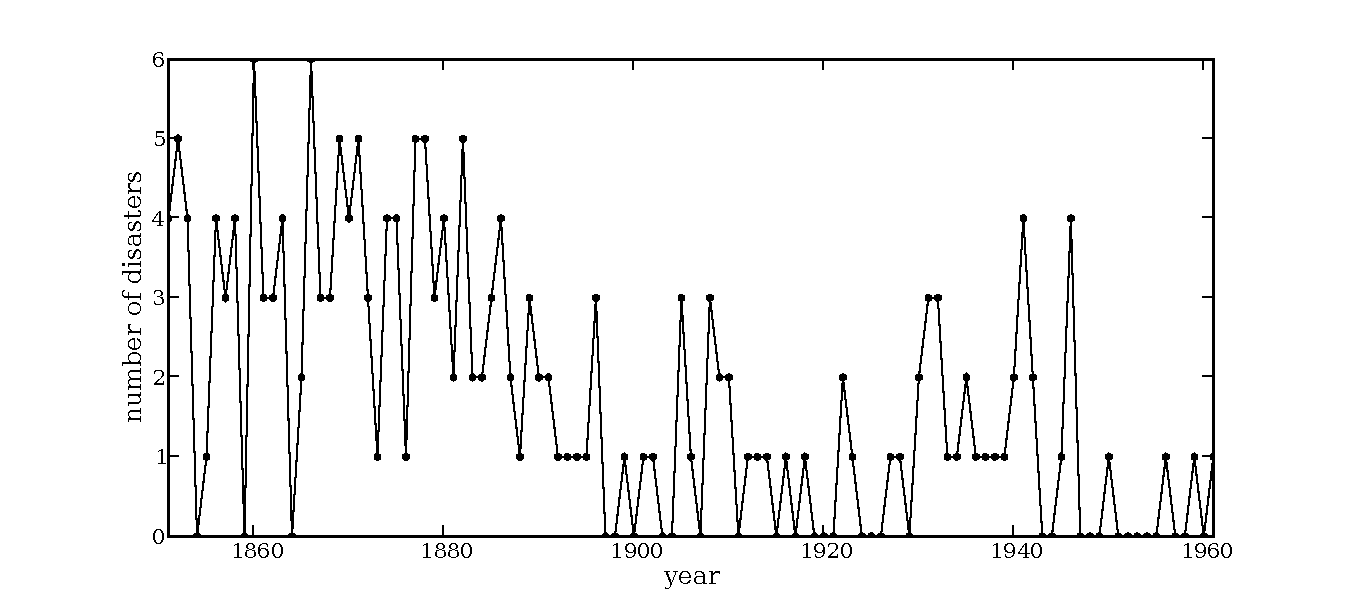
\includegraphics{disasterts.pdf}
\caption{Recorded coal mining disasters in the UK.}\label{tutorial:disasters-figure}\end{figure}

Occurrences of disasters in the time series is thought to be derived from a Poisson process with a large rate parameter in the early part of the time series, and from one with a smaller rate in the later part. We are interested in locating the change point in the series, which perhaps is related to changes in mining safety regulations.

We represent our conceptual model formally as a statistical model:
\phantomsection\label{tutorial:equation-disaster_model}\begin{gather}
\begin{split}     \begin{array}{ccc}  (D_t | s, e, l) \sim\text{Poisson}\left(r_t\right), & r_t=\left\{\begin{array}{lll}             e &\text{if}& t< s\\ l &\text{if}& t\ge s             \end{array}\right.,&t\in[t_l,t_h]\\         s\sim \text{Discrete Uniform}(t_l, t_h)\\         e\sim \text{Exponential}(r_e)\\         l\sim \text{Exponential}(r_l)     \end{array}\end{split}\label{tutorial-disaster_model}
\end{gather}
The symbols are defined as:
\begin{itemize}
\item {} 
$D_t$: The number of disasters in year $t$.

\item {} 
$r_t$: The rate parameter of the Poisson distribution of disasters in year $t$.

\item {} 
$s$: The year in which the rate parameter changes (the switchpoint).

\item {} 
$e$: The rate parameter before the switchpoint $s$.

\item {} 
$l$: The rate parameter after the switchpoint $s$.

\item {} 
$t_l$, $t_h$: The lower and upper boundaries of year $t$.

\item {} 
$r_e$, $r_l$: The rate parameters of the priors of the early and late rates, respectively.

\end{itemize}

Because we have defined $D$ by its dependence on $S$, $e$ and $l$, the latter three are known as the ``parents'' of $D$ and $D$ is called their ``child''. Similarly, the parents of $s$ are $t_l$ and $t_h$, and $s$ is the child of $t_l$ and $t_h$.


\section{Two types of variables}
\label{tutorial:two-types-of-variables}
At the model-specification stage (before the data are observed), $D$, $s$, $e$, \code{rate} and $l$ are all random variables. Bayesian ``random'' variables have not necessarily arisen from a physical random process. The Bayesian interpretation of probability is \emph{epistemic}, meaning random variable $x$`s probability distribution $p(x)$ represents our knowledge and uncertainty about $x$`s value {\hyperref[references:jaynes-2003]{{[}Jaynes\_2003{]}}}. Candidate values of $x$ for which $p(x)$ is high are relatively more probable, given what we know. Random variables are represented in PyMC by the classes \code{Stochastic} and \code{Deterministic}.

The only \code{Deterministic} in the model is \code{rate}. If we knew the values of \code{rate}`s parents ($s$, $l$ and $e$), we could compute the value of \code{rate} exactly. A \code{Deterministic} like \code{rate} is defined by a mathematical function that returns its value given values for its parents. \code{Deterministic} variables are sometimes called the \emph{systemic} part of the model. The nomenclature is a bit confusing, because these objects usually represent random variables; since the parents of \code{rate} are random, \code{rate} is random also. A more descriptive (though more awkward) name for this class would be \code{DeterminedByValuesOfParents}.
\begin{description}
\item[{On the other hand, even if the values of the parents of variables \code{switchpoint}, \emph{disasters} (before observing the data), \code{early\_mean}}] \leavevmode
or \code{late\_mean} were known, we would still be uncertain of their values. These variables are characterized by probability distributions that express how plausible their candidate values are, given values for their parents. The \code{Stochastic} class represents these variables. A more descriptive name for these objects might be \code{RandomEvenGivenValuesOfParents}.

\end{description}

We can represent model \eqref{tutorial-disaster_model} in a file called \code{disaster\_model.py} (the actual file can be found in \code{pymc/examples/}) as follows. First, we import the PyMC and NumPy namespaces:

\begin{Verbatim}[commandchars=\\\{\}]
\PYG{k+kn}{from} \PYG{n+nn}{pymc} \PYG{k+kn}{import} \PYG{n}{DiscreteUniform}\PYG{p}{,} \PYG{n}{Exponential}\PYG{p}{,} \PYG{n}{deterministic}\PYG{p}{,} \PYG{n}{Poisson}\PYG{p}{,} \PYG{n}{Uniform}
\PYG{k+kn}{import} \PYG{n+nn}{numpy} \PYG{k+kn}{as} \PYG{n+nn}{np}
\end{Verbatim}

Notice that from \code{pymc} we have only imported a select few objects that are needed for this particular model, whereas the entire \code{numpy} namespace has been imported, and conveniently given a shorter name. Objects from NumPy are subsequently accessed by prefixing \code{np.} to the name. Either approach is acceptable.

Next, we enter the actual data values into an array:

\begin{Verbatim}[commandchars=\\\{\}]
\PYG{n}{disasters\PYGZus{}array} \PYG{o}{=}   \PYGZbs{}
     \PYG{n}{numpy}\PYG{o}{.}\PYG{n}{array}\PYG{p}{(}\PYG{p}{[} \PYG{l+m+mi}{4}\PYG{p}{,} \PYG{l+m+mi}{5}\PYG{p}{,} \PYG{l+m+mi}{4}\PYG{p}{,} \PYG{l+m+mi}{0}\PYG{p}{,} \PYG{l+m+mi}{1}\PYG{p}{,} \PYG{l+m+mi}{4}\PYG{p}{,} \PYG{l+m+mi}{3}\PYG{p}{,} \PYG{l+m+mi}{4}\PYG{p}{,} \PYG{l+m+mi}{0}\PYG{p}{,} \PYG{l+m+mi}{6}\PYG{p}{,} \PYG{l+m+mi}{3}\PYG{p}{,} \PYG{l+m+mi}{3}\PYG{p}{,} \PYG{l+m+mi}{4}\PYG{p}{,} \PYG{l+m+mi}{0}\PYG{p}{,} \PYG{l+m+mi}{2}\PYG{p}{,} \PYG{l+m+mi}{6}\PYG{p}{,}
                   \PYG{l+m+mi}{3}\PYG{p}{,} \PYG{l+m+mi}{3}\PYG{p}{,} \PYG{l+m+mi}{5}\PYG{p}{,} \PYG{l+m+mi}{4}\PYG{p}{,} \PYG{l+m+mi}{5}\PYG{p}{,} \PYG{l+m+mi}{3}\PYG{p}{,} \PYG{l+m+mi}{1}\PYG{p}{,} \PYG{l+m+mi}{4}\PYG{p}{,} \PYG{l+m+mi}{4}\PYG{p}{,} \PYG{l+m+mi}{1}\PYG{p}{,} \PYG{l+m+mi}{5}\PYG{p}{,} \PYG{l+m+mi}{5}\PYG{p}{,} \PYG{l+m+mi}{3}\PYG{p}{,} \PYG{l+m+mi}{4}\PYG{p}{,} \PYG{l+m+mi}{2}\PYG{p}{,} \PYG{l+m+mi}{5}\PYG{p}{,}
                   \PYG{l+m+mi}{2}\PYG{p}{,} \PYG{l+m+mi}{2}\PYG{p}{,} \PYG{l+m+mi}{3}\PYG{p}{,} \PYG{l+m+mi}{4}\PYG{p}{,} \PYG{l+m+mi}{2}\PYG{p}{,} \PYG{l+m+mi}{1}\PYG{p}{,} \PYG{l+m+mi}{3}\PYG{p}{,} \PYG{l+m+mi}{2}\PYG{p}{,} \PYG{l+m+mi}{2}\PYG{p}{,} \PYG{l+m+mi}{1}\PYG{p}{,} \PYG{l+m+mi}{1}\PYG{p}{,} \PYG{l+m+mi}{1}\PYG{p}{,} \PYG{l+m+mi}{1}\PYG{p}{,} \PYG{l+m+mi}{3}\PYG{p}{,} \PYG{l+m+mi}{0}\PYG{p}{,} \PYG{l+m+mi}{0}\PYG{p}{,}
                   \PYG{l+m+mi}{1}\PYG{p}{,} \PYG{l+m+mi}{0}\PYG{p}{,} \PYG{l+m+mi}{1}\PYG{p}{,} \PYG{l+m+mi}{1}\PYG{p}{,} \PYG{l+m+mi}{0}\PYG{p}{,} \PYG{l+m+mi}{0}\PYG{p}{,} \PYG{l+m+mi}{3}\PYG{p}{,} \PYG{l+m+mi}{1}\PYG{p}{,} \PYG{l+m+mi}{0}\PYG{p}{,} \PYG{l+m+mi}{3}\PYG{p}{,} \PYG{l+m+mi}{2}\PYG{p}{,} \PYG{l+m+mi}{2}\PYG{p}{,} \PYG{l+m+mi}{0}\PYG{p}{,} \PYG{l+m+mi}{1}\PYG{p}{,} \PYG{l+m+mi}{1}\PYG{p}{,} \PYG{l+m+mi}{1}\PYG{p}{,}
                   \PYG{l+m+mi}{0}\PYG{p}{,} \PYG{l+m+mi}{1}\PYG{p}{,} \PYG{l+m+mi}{0}\PYG{p}{,} \PYG{l+m+mi}{1}\PYG{p}{,} \PYG{l+m+mi}{0}\PYG{p}{,} \PYG{l+m+mi}{0}\PYG{p}{,} \PYG{l+m+mi}{0}\PYG{p}{,} \PYG{l+m+mi}{2}\PYG{p}{,} \PYG{l+m+mi}{1}\PYG{p}{,} \PYG{l+m+mi}{0}\PYG{p}{,} \PYG{l+m+mi}{0}\PYG{p}{,} \PYG{l+m+mi}{0}\PYG{p}{,} \PYG{l+m+mi}{1}\PYG{p}{,} \PYG{l+m+mi}{1}\PYG{p}{,} \PYG{l+m+mi}{0}\PYG{p}{,} \PYG{l+m+mi}{2}\PYG{p}{,}
                   \PYG{l+m+mi}{3}\PYG{p}{,} \PYG{l+m+mi}{3}\PYG{p}{,} \PYG{l+m+mi}{1}\PYG{p}{,} \PYG{l+m+mi}{1}\PYG{p}{,} \PYG{l+m+mi}{2}\PYG{p}{,} \PYG{l+m+mi}{1}\PYG{p}{,} \PYG{l+m+mi}{1}\PYG{p}{,} \PYG{l+m+mi}{1}\PYG{p}{,} \PYG{l+m+mi}{1}\PYG{p}{,} \PYG{l+m+mi}{2}\PYG{p}{,} \PYG{l+m+mi}{4}\PYG{p}{,} \PYG{l+m+mi}{2}\PYG{p}{,} \PYG{l+m+mi}{0}\PYG{p}{,} \PYG{l+m+mi}{0}\PYG{p}{,} \PYG{l+m+mi}{1}\PYG{p}{,} \PYG{l+m+mi}{4}\PYG{p}{,}
                   \PYG{l+m+mi}{0}\PYG{p}{,} \PYG{l+m+mi}{0}\PYG{p}{,} \PYG{l+m+mi}{0}\PYG{p}{,} \PYG{l+m+mi}{1}\PYG{p}{,} \PYG{l+m+mi}{0}\PYG{p}{,} \PYG{l+m+mi}{0}\PYG{p}{,} \PYG{l+m+mi}{0}\PYG{p}{,} \PYG{l+m+mi}{0}\PYG{p}{,} \PYG{l+m+mi}{0}\PYG{p}{,} \PYG{l+m+mi}{1}\PYG{p}{,} \PYG{l+m+mi}{0}\PYG{p}{,} \PYG{l+m+mi}{0}\PYG{p}{,} \PYG{l+m+mi}{1}\PYG{p}{,} \PYG{l+m+mi}{0}\PYG{p}{,} \PYG{l+m+mi}{1}\PYG{p}{]}\PYG{p}{)}
\end{Verbatim}

Note that you don't have to type in this entire array to follow along; the code is available in the source tree, in \code{this example script}.  Next, we create the switchpoint variable \code{switchpoint}

\begin{Verbatim}[commandchars=\\\{\}]
\PYG{n}{switchpoint} \PYG{o}{=} \PYG{n}{DiscreteUniform}\PYG{p}{(}\PYG{l+s}{'}\PYG{l+s}{switchpoint}\PYG{l+s}{'}\PYG{p}{,} \PYG{n}{lower}\PYG{o}{=}\PYG{l+m+mi}{0}\PYG{p}{,} \PYG{n}{upper}\PYG{o}{=}\PYG{l+m+mi}{110}\PYG{p}{,} \PYG{n}{doc}\PYG{o}{=}\PYG{l+s}{'}\PYG{l+s}{Switchpoint[year]}\PYG{l+s}{'}\PYG{p}{)}
\end{Verbatim}
\begin{description}
\item[{\code{DiscreteUniform} is a subclass of \code{Stochastic} that represents uniformly-distributed discrete variables. Use of this distribution suggests that we have no preference \code{a priori} regarding the location of the switchpoint; all values are equally likely. Now we create the exponentially-distributed variables \code{early\_mean}}] \leavevmode
and \code{late\_mean} for the early and late Poisson

\end{description}

rates, respectively:

\begin{Verbatim}[commandchars=\\\{\}]
\PYG{n}{early\PYGZus{}mean} \PYG{o}{=} \PYG{n}{Exponential}\PYG{p}{(}\PYG{l+s}{'}\PYG{l+s}{early\PYGZus{}mean}\PYG{l+s}{'}\PYG{p}{,}\PYG{n}{beta}\PYG{o}{=}\PYG{l+m+mf}{1.}\PYG{p}{)}
\PYG{n}{late\PYGZus{}mean} \PYG{o}{=} \PYG{n}{Exponential}\PYG{p}{(}\PYG{l+s}{'}\PYG{l+s}{late\PYGZus{}mean}\PYG{l+s}{'}\PYG{p}{,}\PYG{n}{beta}\PYG{o}{=}\PYG{l+m+mf}{1.}\PYG{p}{)}
\end{Verbatim}
\begin{description}
\item[{Next, we define the variable \code{rate}, which selects the early rate \code{early\_mean}}] \leavevmode
for times before \code{switchpoint} and the late rate \code{late\_mean} for times after \code{switchpoint}. We create \code{rate} using the \code{deterministic} decorator, which converts the ordinary Python function \code{rate} into a \code{Deterministic} object.:

\begin{Verbatim}[commandchars=@\[\]]
@PYGZat[]deterministic(plot=False)
     def rate(s=switchpoint, e=early@_mean, l=late@_mean):
         ''' Concatenate Poisson means '''
         out = empty(len(disasters@_array))
         out@PYGZlb[]:s@PYGZrb[] = e
         out@PYGZlb[]s:@PYGZrb[] = l
         return out
\end{Verbatim}

\end{description}

The last step is to define the number of disasters \code{disasters}. This is a stochastic variable but unlike \code{switchpoint}, \code{early\_mean}
{}` and \code{late\_mean} we have observed its value. To express this, we set the argument \code{observed} to \code{True} (it is set to \code{False} by default). This tells PyMC that this object's value should not be changed:

\begin{Verbatim}[commandchars=\\\{\}]
\PYG{n}{disasters} \PYG{o}{=} \PYG{n}{Poisson}\PYG{p}{(}\PYG{l+s}{'}\PYG{l+s}{disasters}\PYG{l+s}{'}\PYG{p}{,} \PYG{n}{mu}\PYG{o}{=}\PYG{n}{rate}\PYG{p}{,} \PYG{n}{value}\PYG{o}{=}\PYG{n}{disasters\PYGZus{}array}\PYG{p}{,} \PYG{n}{observed}\PYG{o}{=}\PYG{n+nb+bp}{True}\PYG{p}{)}
\end{Verbatim}


\subsection{Why are data and unknown variables represented by the same object?}
\label{tutorial:why-are-data-and-unknown-variables-represented-by-the-same-object}
Since its represented by a \code{Stochastic} object, \emph{disasters} is defined by its dependence on its parent \code{rate} even though its value is fixed. This isn't just a quirk of PyMC's syntax; Bayesian hierarchical notation itself makes no distinction between random variables and data. The reason is simple: to use Bayes' theorem to compute the posterior $p(e,s,l \mid D)$ of model \eqref{tutorial-disaster_model}, we require the likelihood $p(D \mid e,s,l)$. Even though \emph{disasters}`s value is known and fixed, we need to formally assign it a probability distribution as if it were a random variable. Remember, the likelihood and the probability function are essentially the same, except that the former is regarded as a function of the parameters and the latter as a function of the data.

This point can be counterintuitive at first, as many peoples' instinct is to regard data as fixed a priori and unknown variables as dependent on the data. One way to understand this is to think of statistical models like \eqref{tutorial-disaster_model} as predictive models for data, or as models of the processes that gave rise to data. Before observing the value of \emph{disasters}, we could have sampled from its prior predictive distribution $p(D)$ (\emph{i.e.} the marginal distribution of the data) as follows:
\begin{itemize}
\item {} 
Sample \code{early\_mean}

\end{itemize}
\begin{description}
\item[{, \code{switchpoint} and \code{late\_mean} from their priors.}] \leavevmode\begin{itemize}
\item {} 
Sample \emph{disasters} conditional on these values.

\end{itemize}

\end{description}

Even after we observe the value of \emph{disasters}, we need to use this process model to make inferences about \code{early\_mean}
, \code{switchpoint} and \code{late\_mean} because its the only information we have about how the variables are related.


\section{Parents and children}
\label{tutorial:parents-and-children}
We have above created a PyMC probability model, which is simply a linked collection of variables. To see the nature of the links, import or run \code{disaster\_model.py} and examine \code{switchpoint}`s \code{parents} attribute from the Python prompt:

\begin{Verbatim}[commandchars=\\\{\}]
\PYG{g+gp}{\textgreater{}\textgreater{}\textgreater{} }\PYG{k+kn}{from} \PYG{n+nn}{pymc.examples} \PYG{k+kn}{import} \PYG{n}{disaster\PYGZus{}model}
\PYG{g+gp}{\textgreater{}\textgreater{}\textgreater{} }\PYG{n}{disaster\PYGZus{}model}\PYG{o}{.}\PYG{n}{switchpoint}\PYG{o}{.}\PYG{n}{parents}
\PYG{g+go}{\PYGZob{}'lower': 0, 'upper': 110\PYGZcb{}}
\end{Verbatim}

The \code{parents} dictionary shows us the distributional parameters of \code{switchpoint}, which are constants. Now let's examine \emph{disasters}`s parents:

\begin{Verbatim}[commandchars=\\\{\}]
\PYG{g+gp}{\textgreater{}\textgreater{}\textgreater{} }\PYG{n}{disaster\PYGZus{}model}\PYG{o}{.}\PYG{n}{disasters}\PYG{o}{.}\PYG{n}{parents}
\PYG{g+go}{\PYGZob{}'early\PYGZus{}mean': \textless{}pymc.distributions.Exponential 'early\PYGZus{}mean' at 0x1065acf50\textgreater{},}
\PYG{g+go}{      'late\PYGZus{}mean': \textless{}pymc.distributions.Exponential 'late\PYGZus{}mean' at 0x1065acfd0\textgreater{},}
\PYG{g+go}{      'switchpoint': \textless{}pymc.distributions.DiscreteUniform 'switchpoint' at 0x1065ace90\textgreater{}\PYGZcb{}}
\end{Verbatim}

We are using \code{rate} as a distributional parameter of \emph{disasters} (\emph{i.e.} \code{rate} is \emph{disasters}`s parent). \emph{disasters} internally labels \code{rate} as \code{mu}, meaning \code{rate} plays the role of the rate parameter in \emph{disasters}`s Poisson distribution. Now examine \code{rate}`s \code{children} attribute:

\begin{Verbatim}[commandchars=\\\{\}]
\PYG{g+gp}{\textgreater{}\textgreater{}\textgreater{} }\PYG{n}{disaster\PYGZus{}model}\PYG{o}{.}\PYG{n}{rate}\PYG{o}{.}\PYG{n}{children}
\PYG{g+go}{set([\textless{}pymc.distributions.Poisson 'D' at 0x3e51290\textgreater{}])}
\end{Verbatim}

Because \emph{disasters} considers \code{rate} its parent, \code{rate} considers \emph{disasters} its child. Unlike \code{parents}, \code{children} is a set (an unordered collection of objects); variables do not associate their children with any particular distributional role. Try examining the \code{parents} and \code{children} attributes of the other parameters in the model.
\begin{description}
\item[{The following \emph{directed acyclic graph} is a visualization of the parent-child relationships in the model. Unobserved stochastic variables \code{switchpoint}, \code{early\_mean}}] \leavevmode
and \code{late\_mean} are open ellipses, observed stochastic variable \emph{disasters} is a filled ellipse and deterministic variable \code{rate} is a triangle. Arrows point from parent to child and display the label that the child assigns to the parent. See section {\hyperref[modelbuilding:graphical]{\emph{Graphing models}}} for more details.

\end{description}
\begin{figure}[htbp]
\centering
\capstart

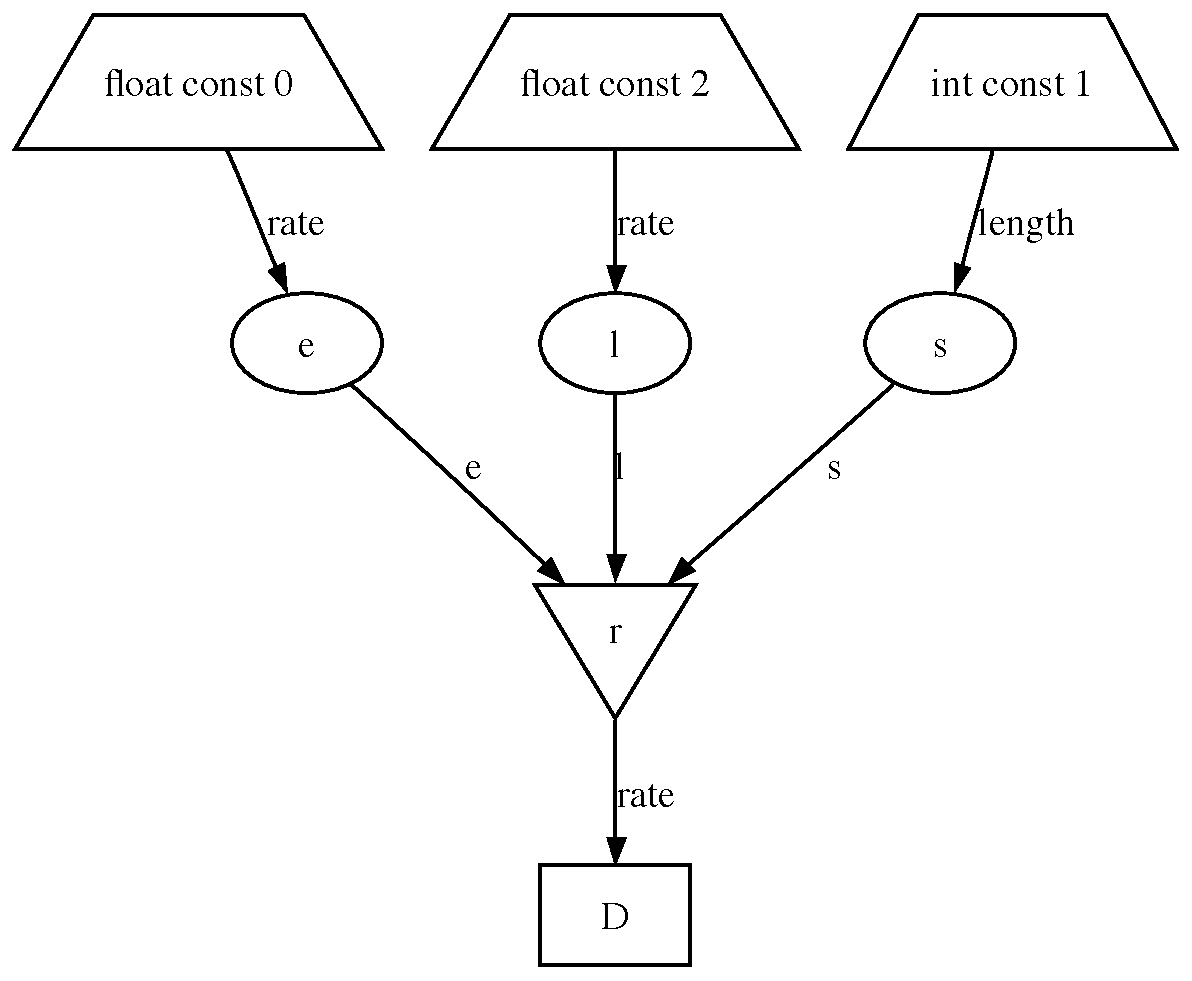
\includegraphics{DisasterModel2.pdf}
\caption{Directed acyclic graph of the relationships in the coal mining disaster model example.}\label{tutorial:dag}\end{figure}

As the examples above have shown, pymc objects need to have a name assigned, such as \code{switchpoint}, \code{early\_mean} or \code{late\_mean}. These names are used for storage and post-processing:
\begin{itemize}
\item {} 
as keys in on-disk databases,

\item {} 
as node labels in model graphs,

\item {} 
as axis labels in plots of traces,

\item {} 
as table labels in summary statistics.

\end{itemize}

A model instantiated with variables having identical names raises an error to avoid name conflicts in the database storing the traces. In general however, pymc uses references to the objects themselves, not their names, to identify variables.


\section{Variables' values and log-probabilities}
\label{tutorial:variables-values-and-log-probabilities}
All PyMC variables have an attribute called \code{value} that stores the current value of that variable. Try examining \emph{disasters}`s value, and you'll see the initial value we provided for it:

\begin{Verbatim}[commandchars=\\\{\}]
\PYG{g+gp}{\textgreater{}\textgreater{}\textgreater{} }\PYG{n}{disaster\PYGZus{}model}\PYG{o}{.}\PYG{n}{disasters}\PYG{o}{.}\PYG{n}{value}
\PYG{g+go}{array([4, 5, 4, 0, 1, 4, 3, 4, 0, 6, 3, 3, 4, 0, 2, 6, 3, 3, 5, 4, 5, 3, 1,}
\PYG{g+go}{       4, 4, 1, 5, 5, 3, 4, 2, 5, 2, 2, 3, 4, 2, 1, 3, 2, 2, 1, 1, 1, 1, 3,}
\PYG{g+go}{       0, 0, 1, 0, 1, 1, 0, 0, 3, 1, 0, 3, 2, 2, 0, 1, 1, 1, 0, 1, 0, 1, 0,}
\PYG{g+go}{       0, 0, 2, 1, 0, 0, 0, 1, 1, 0, 2, 3, 3, 1, 1, 2, 1, 1, 1, 1, 2, 4, 2,}
\PYG{g+go}{       0, 0, 1, 4, 0, 0, 0, 1, 0, 0, 0, 0, 0, 1, 0, 0, 1, 0, 1])}
\end{Verbatim}

If you check the values of \code{early\_mean}, \code{switchpoint} and \code{late\_mean}, you'll see random initial values generated by PyMC:

\begin{Verbatim}[commandchars=\\\{\}]
\PYG{g+gp}{\textgreater{}\textgreater{}\textgreater{} }\PYG{n}{disaster\PYGZus{}model}\PYG{o}{.}\PYG{n}{switchpoint}\PYG{o}{.}\PYG{n}{value}
\PYG{g+go}{44}

\PYG{g+gp}{\textgreater{}\textgreater{}\textgreater{} }\PYG{n}{disaster\PYGZus{}model}\PYG{o}{.}\PYG{n}{early\PYGZus{}mean}\PYG{o}{.}\PYG{n}{value}
\PYG{g+go}{0.33464706250079584}

\PYG{g+gp}{\textgreater{}\textgreater{}\textgreater{} }\PYG{n}{disaster\PYGZus{}model}\PYG{o}{.}\PYG{n}{late\PYGZus{}mean}\PYG{o}{.}\PYG{n}{value}
\PYG{g+go}{2.6491936762267811}
\end{Verbatim}

Of course, since these are \code{Stochastic} elements, your values will be different than these. If you check \code{rate}`s value, you'll see an array whose first \code{switchpoint} elements are \code{early\_mean} (here 0.33464706), and whose remaining elements are \code{late\_mean} (here 2.64919368):

\begin{Verbatim}[commandchars=\\\{\}]
\PYG{g+gp}{\textgreater{}\textgreater{}\textgreater{} }\PYG{n}{disaster\PYGZus{}model}\PYG{o}{.}\PYG{n}{rate}\PYG{o}{.}\PYG{n}{value}
\PYG{g+go}{array([ 0.33464706,  0.33464706,  0.33464706,  0.33464706,  0.33464706,}
\PYG{g+go}{        0.33464706,  0.33464706,  0.33464706,  0.33464706,  0.33464706,}
\PYG{g+go}{        0.33464706,  0.33464706,  0.33464706,  0.33464706,  0.33464706,}
\PYG{g+go}{        0.33464706,  0.33464706,  0.33464706,  0.33464706,  0.33464706,}
\PYG{g+go}{        0.33464706,  0.33464706,  0.33464706,  0.33464706,  0.33464706,}
\PYG{g+go}{        0.33464706,  0.33464706,  0.33464706,  0.33464706,  0.33464706,}
\PYG{g+go}{        0.33464706,  0.33464706,  0.33464706,  0.33464706,  0.33464706,}
\PYG{g+go}{        0.33464706,  0.33464706,  0.33464706,  0.33464706,  0.33464706,}
\PYG{g+go}{        0.33464706,  0.33464706,  0.33464706,  0.33464706,  2.64919368,}
\PYG{g+go}{        2.64919368,  2.64919368,  2.64919368,  2.64919368,  2.64919368,}
\PYG{g+go}{        2.64919368,  2.64919368,  2.64919368,  2.64919368,  2.64919368,}
\PYG{g+go}{        2.64919368,  2.64919368,  2.64919368,  2.64919368,  2.64919368,}
\PYG{g+go}{        2.64919368,  2.64919368,  2.64919368,  2.64919368,  2.64919368,}
\PYG{g+go}{        2.64919368,  2.64919368,  2.64919368,  2.64919368,  2.64919368,}
\PYG{g+go}{        2.64919368,  2.64919368,  2.64919368,  2.64919368,  2.64919368,}
\PYG{g+go}{        2.64919368,  2.64919368,  2.64919368,  2.64919368,  2.64919368,}
\PYG{g+go}{        2.64919368,  2.64919368,  2.64919368,  2.64919368,  2.64919368,}
\PYG{g+go}{        2.64919368,  2.64919368,  2.64919368,  2.64919368,  2.64919368,}
\PYG{g+go}{        2.64919368,  2.64919368,  2.64919368,  2.64919368,  2.64919368,}
\PYG{g+go}{        2.64919368,  2.64919368,  2.64919368,  2.64919368,  2.64919368,}
\PYG{g+go}{        2.64919368,  2.64919368,  2.64919368,  2.64919368,  2.64919368,}
\PYG{g+go}{        2.64919368,  2.64919368,  2.64919368,  2.64919368,  2.64919368])}
\end{Verbatim}

To compute its value, \code{rate} calls the function we used to create it, passing in the values of its parents.

\code{Stochastic} objects can evaluate their probability mass or density functions at their current values given the values of their parents. The logarithm of a stochastic object's probability mass or density can be accessed via the \code{logp} attribute. For vector-valued variables like \emph{disasters}, the \code{logp} attribute returns the sum of the logarithms of the joint probability or density of all elements of the value. Try examining \code{switchpoint}`s and \emph{disasters}`s log-probabilities and \code{early\_mean}
`s and \code{late\_mean}`s log-densities:

\begin{Verbatim}[commandchars=\\\{\}]
\PYG{g+gp}{\textgreater{}\textgreater{}\textgreater{} }\PYG{n}{disaster\PYGZus{}model}\PYG{o}{.}\PYG{n}{switchpoint}\PYG{o}{.}\PYG{n}{logp}
\PYG{g+go}{-4.7095302013123339}

\PYG{g+gp}{\textgreater{}\textgreater{}\textgreater{} }\PYG{n}{disaster\PYGZus{}model}\PYG{o}{.}\PYG{n}{disasters}\PYG{o}{.}\PYG{n}{logp}
\PYG{g+go}{-1080.5149888046033}

\PYG{g+gp}{\textgreater{}\textgreater{}\textgreater{} }\PYG{n}{disaster\PYGZus{}model}\PYG{o}{.}\PYG{n}{early\PYGZus{}mean}\PYG{o}{.}\PYG{n}{logp}
\PYG{g+go}{-0.33464706250079584}

\PYG{g+gp}{\textgreater{}\textgreater{}\textgreater{} }\PYG{n}{disaster\PYGZus{}model}\PYG{o}{.}\PYG{n}{late\PYGZus{}mean}\PYG{o}{.}\PYG{n}{logp}
\PYG{g+go}{-2.6491936762267811}
\end{Verbatim}

\code{Stochastic} objects need to call an internal function to compute their \code{logp} attributes, as \code{rate} needed to call an internal function to compute its value. Just as we created \code{rate} by decorating a function that computes its value, it's possible to create custom \code{Stochastic} objects by decorating functions that compute their log-probabilities or densities (see chapter {\hyperref[modelbuilding:chap-modelbuilding]{\emph{Building models}}}). Users are thus not limited to the set of of statistical distributions provided by PyMC.


\subsection{Using Variables as parents of other Variables}
\label{tutorial:using-variables-as-parents-of-other-variables}
Let's take a closer look at our definition of \code{rate}:

\begin{Verbatim}[commandchars=@\[\]]
@PYGZat[]deterministic(plot=False)
     def rate(s=switchpoint, e=early@_mean, l=late@_mean):
         ''' Concatenate Poisson means '''
         out = empty(len(disasters@_array))
         out@PYGZlb[]:s@PYGZrb[] = e
         out@PYGZlb[]s:@PYGZrb[] = l
         return out
\end{Verbatim}

The arguments \code{switchpoint}, \code{early\_mean} and \code{late\_mean} are \code{Stochastic} objects, not numbers. If that is so, why aren't errors raised when we attempt to slice array \code{out} up to a \code{Stochastic} object?

Whenever a variable is used as a parent for a child variable, PyMC replaces it with its \code{value} attribute when the child's value or log-probability is computed. When \code{rate}`s value is recomputed, \code{s.value} is passed to the function as argument \code{switchpoint}. To see the values of the parents of \code{rate} all together, look at \code{rate.parents.value}.


\section{Fitting the model with MCMC}
\label{tutorial:fitting-the-model-with-mcmc}
PyMC provides several objects that fit probability models (linked collections of variables) like ours. The primary such object, \code{MCMC}, fits models with a Markov chain Monte Carlo algorithm {\hyperref[references:gamerman-1997]{{[}Gamerman\_1997{]}}}. To create an \code{MCMC} object to handle our model, import \code{disaster\_model.py} and use it as an argument for \code{MCMC}:

\begin{Verbatim}[commandchars=\\\{\}]
\PYG{g+gp}{\textgreater{}\textgreater{}\textgreater{} }\PYG{k+kn}{from} \PYG{n+nn}{pymc.examples} \PYG{k+kn}{import} \PYG{n}{disaster\PYGZus{}model}
\PYG{g+gp}{\textgreater{}\textgreater{}\textgreater{} }\PYG{k+kn}{from} \PYG{n+nn}{pymc} \PYG{k+kn}{import} \PYG{n}{MCMC}
\PYG{g+gp}{\textgreater{}\textgreater{}\textgreater{} }\PYG{n}{M} \PYG{o}{=} \PYG{n}{MCMC}\PYG{p}{(}\PYG{n}{disaster\PYGZus{}model}\PYG{p}{)}
\end{Verbatim}

In this case \code{M} will expose variables \code{switchpoint}, \code{early\_mean}, \code{late\_mean} and \code{disasters} as attributes; that is, \code{M.switchpoint} will be the same object as \code{disaster\_model.switchpoint}.

To run the sampler, call the MCMC object's \code{sample()} (or \code{isample()}, for interactive sampling) method with arguments for the number of iterations, burn-in length, and thinning interval (if desired):

\begin{Verbatim}[commandchars=\\\{\}]
\PYG{g+gp}{\textgreater{}\textgreater{}\textgreater{} }\PYG{n}{M}\PYG{o}{.}\PYG{n}{sample}\PYG{p}{(}\PYG{n+nb}{iter}\PYG{o}{=}\PYG{l+m+mi}{10000}\PYG{p}{,} \PYG{n}{burn}\PYG{o}{=}\PYG{l+m+mi}{1000}\PYG{p}{,} \PYG{n}{thin}\PYG{o}{=}\PYG{l+m+mi}{10}\PYG{p}{)}
\end{Verbatim}

After a few seconds, you should see that sampling has finished normally. The model has been fitted.


\subsection{What does it mean to fit a model?}
\label{tutorial:what-does-it-mean-to-fit-a-model}
\emph{Fitting} a model means characterizing its posterior distribution somehow. In this case, we are trying to represent the posterior $p(s,e,l|D)$ by a set of joint samples from it. To produce these samples, the MCMC sampler randomly updates the values of \code{switchpoint}, \code{early\_mean} and \code{late\_mean} according to the Metropolis-Hastings algorithm {\hyperref[references:gelman-2004]{{[}Gelman\_2004{]}}} over a specified number of iterations (\code{iter}).

As the number of samples grows sufficiently large, the MCMC distributions of \code{switchpoint}, \code{early\_mean} and \code{late\_mean} converge to their joint stationary distribution. In other words, their values can be considered as random draws from the posterior $p(s,e,l|D)$. PyMC assumes that the \code{burn} parameter specifies a \emph{sufficiently large} number of iterations for the algorithm to converge, so it is up to the user to verify that this is the case (see chapter {\hyperref[modelchecking:chap-modelchecking]{\emph{Model checking and diagnostics}}}). Consecutive values sampled from \code{switchpoint}, \code{early\_mean} and \code{late\_mean} are always serially dependent, since it is a Markov chain. MCMC often results in strong autocorrelation among samples that can result in imprecise posterior inference. To circumvent this, it is useful to thin the sample by only retaining every \emph{k} th sample, where $k$ is an integer value. This thinning interval is passed to the sampler via the \code{thin} argument.

If you are not sure ahead of time what values to choose for the \code{burn} and \code{thin} parameters, you may want to retain all the MCMC samples, that is to set \code{burn=0} and \code{thin=1}, and then discard the \emph{burn-in period} and thin the samples after examining the traces (the series of samples). See {\hyperref[references:gelman-2004]{{[}Gelman\_2004{]}}} for general guidance.


\subsection{Accessing the samples}
\label{tutorial:accessing-the-samples}
The output of the MCMC algorithm is a \emph{trace}, the sequence of retained samples for each variable in the model. These traces can be accessed using the \code{trace(name, chain=-1)} method. For example:

\begin{Verbatim}[commandchars=\\\{\}]
\PYG{g+gp}{\textgreater{}\textgreater{}\textgreater{} }\PYG{n}{M}\PYG{o}{.}\PYG{n}{trace}\PYG{p}{(}\PYG{l+s}{'}\PYG{l+s}{switchpoint}\PYG{l+s}{'}\PYG{p}{)}\PYG{p}{[}\PYG{p}{:}\PYG{p}{]}
\PYG{g+go}{array([41, 40, 40, ..., 43, 44, 44])}
\end{Verbatim}

The trace slice \code{{[}start:stop:step{]}} works just like the NumPy array slice. By default, the returned trace array contains the samples from the last call to \code{sample}, that is, \code{chain=-1}, but the trace from previous sampling runs can be retrieved by specifying the correspondent chain index. To return the trace from all chains, simply use \code{chain=None}. \footnote{
Note that the unknown variables \code{switchpoint}, \code{early\_mean}, \code{late\_mean} and \code{rate} will all accrue samples, but \emph{disasters} will not because its value has been observed and is not updated. Hence \emph{disasters} has no trace and calling \code{M.trace('disasters'){[}:{]}} will raise an error.
}


\subsection{Sampling output}
\label{tutorial:sampling-output}
You can examine the marginal posterior of any variable by plotting a histogram of its trace:

\begin{Verbatim}[commandchars=\\\{\}]
\PYG{g+gp}{\textgreater{}\textgreater{}\textgreater{} }\PYG{k+kn}{from} \PYG{n+nn}{pylab} \PYG{k+kn}{import} \PYG{n}{hist}\PYG{p}{,} \PYG{n}{show}
\PYG{g+gp}{\textgreater{}\textgreater{}\textgreater{} }\PYG{n}{hist}\PYG{p}{(}\PYG{n}{M}\PYG{o}{.}\PYG{n}{trace}\PYG{p}{(}\PYG{l+s}{'}\PYG{l+s}{late\PYGZus{}mean}\PYG{l+s}{'}\PYG{p}{)}\PYG{p}{[}\PYG{p}{:}\PYG{p}{]}\PYG{p}{)}
\PYG{g+go}{(array([   8,   52,  565, 1624, 2563, 2105, 1292,  488,  258,   45]),}
\PYG{g+go}{ array([ 0.52721865,  0.60788251,  0.68854637,  0.76921023,  0.84987409,}
\PYG{g+go}{        0.93053795,  1.01120181,  1.09186567,  1.17252953,  1.25319339]),}
\PYG{g+go}{ \textless{}a list of 10 Patch objects\textgreater{})}
\PYG{g+gp}{\textgreater{}\textgreater{}\textgreater{} }\PYG{n}{show}\PYG{p}{(}\PYG{p}{)}
\end{Verbatim}

You should see something like this:
\begin{figure}[htbp]
\centering
\capstart

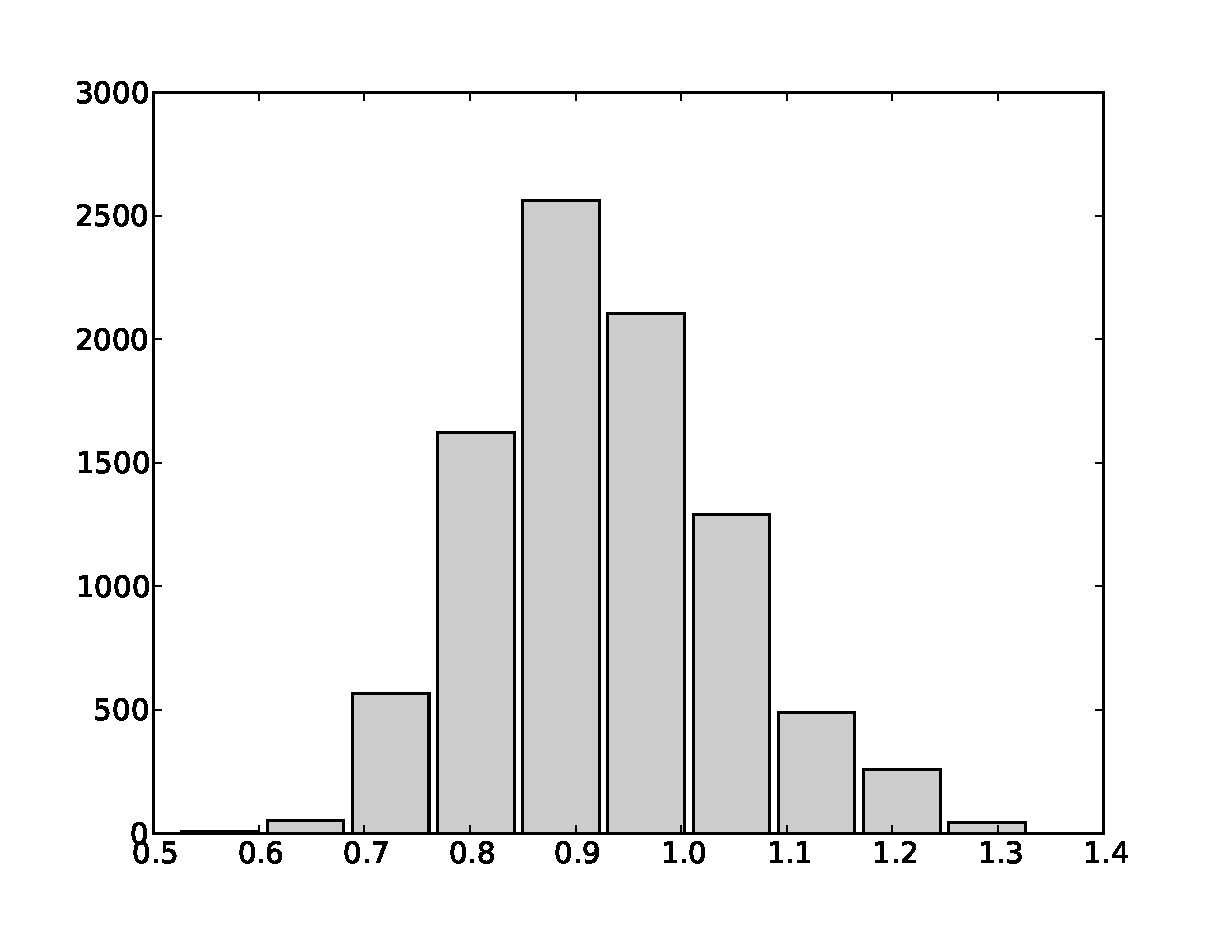
\includegraphics{ltrace.pdf}
\caption{Histogram of the marginal posterior probability of parameter \code{late\_mean}.}\end{figure}

PyMC has its own plotting functionality, via the optional \code{matplotlib} module as noted in the installation notes. The \code{Matplot} module includes a \code{plot} function that takes the model (or a single parameter) as an argument:

\begin{Verbatim}[commandchars=\\\{\}]
\PYG{g+gp}{\textgreater{}\textgreater{}\textgreater{} }\PYG{k+kn}{from} \PYG{n+nn}{pymc.Matplot} \PYG{k+kn}{import} \PYG{n}{plot}
\PYG{g+gp}{\textgreater{}\textgreater{}\textgreater{} }\PYG{n}{plot}\PYG{p}{(}\PYG{n}{M}\PYG{p}{)}
\end{Verbatim}

For each variable in the model, \code{plot} generates a composite figure, such as this one for the switchpoint in the disasters model:
\begin{figure}[htbp]
\centering
\capstart

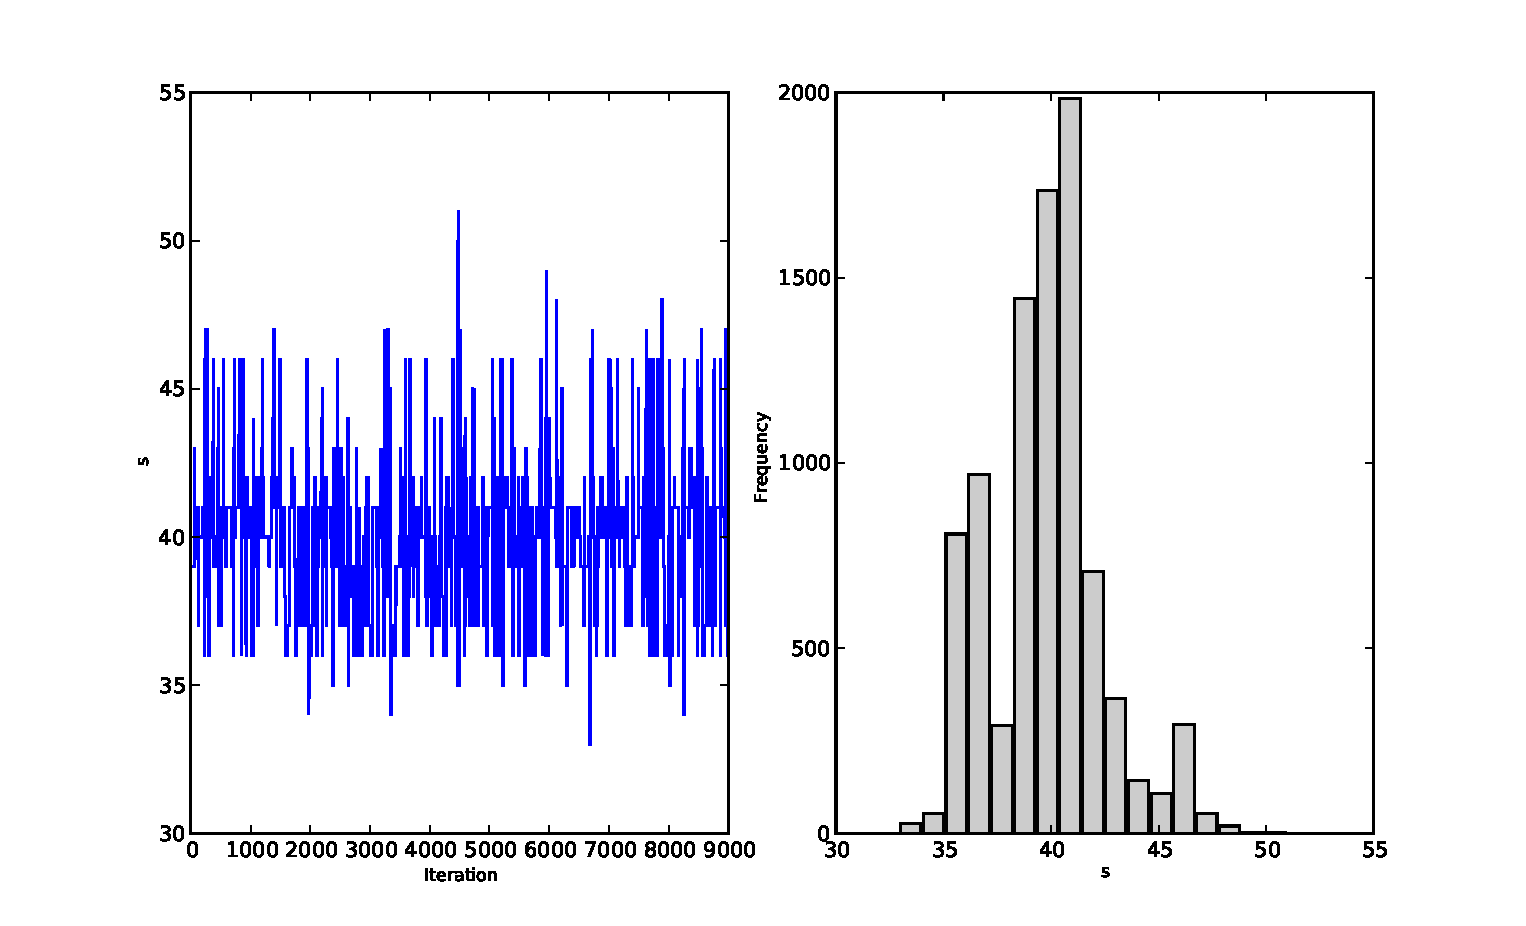
\includegraphics{spost.pdf}
\caption{Temporal series and histogram of the samples drawn for \code{switchpoint}.}\end{figure}

The left-hand pane of this figure shows the temporal series of the samples from \code{switchpoint}, while the right-hand pane shows a histogram of the trace. The trace is useful for evaluating and diagnosing the algorithm's performance (see {\hyperref[references:gelman-1996]{{[}Gelman\_1996{]}}}), while the histogram is useful for visualizing the posterior.

For a non-graphical summary of the posterior, simply call \code{M.stats()}.


\subsection{Imputation of Missing Data}
\label{tutorial:imputation-of-missing-data}
As with most textbook examples, the models we have examined so far assume that the associated data are complete. That is, there are no missing values corresponding to any observations in the dataset. However, many real-world datasets contain one or more missing values, usually due to some logistical problem during the data collection process. The easiest way of dealing with observations that contain missing values is simply to exclude them from the analysis. However, this results in loss of information if an excluded observation contains valid values for other quantities, and can bias results. An alternative is to impute the missing values, based on information in the rest of the model.

For example, consider a survey dataset for some wildlife species:

\begin{tabulary}{\linewidth}{|L|L|L|L|}
\hline
\textbf{
Count
} & \textbf{
Site
} & \textbf{
Observer
} & \textbf{
Temperature
}\\\hline

15
 & 
1
 & 
1
 & 
15
\\\hline

10
 & 
1
 & 
2
 & 
NA
\\\hline

6
 & 
1
 & 
1
 & 
11
\\\hline
\end{tabulary}


Each row contains the number of individuals seen during the survey, along with three covariates: the site on which the survey was conducted, the observer that collected the data, and the temperature during the survey. If we are interested in modelling, say, population size as a function of the count and the associated covariates, it is difficult to accommodate the second observation because the temperature is missing (perhaps the thermometer was broken that day). Ignoring this observation will allow us to fit the model, but it wastes information that is contained in the other covariates.

In a Bayesian modelling framework, missing data are accommodated simply by treating them as unknown model parameters. Values for the missing data $\tilde{y}$ are estimated naturally, using the posterior predictive distribution:
\begin{gather}
\begin{split}p(\tilde{y}|y) = \int p(\tilde{y}|\theta) f(\theta|y) d\theta\end{split}\notag\\\begin{split}\end{split}\notag
\end{gather}
This describes additional data $\tilde{y}$, which may either be considered unobserved data or potential future observations. We can use the posterior predictive distribution to model the likely values of missing data.

Consider the coal mining disasters data introduced previously. Assume that two years of data are missing from the time series; we indicate this in the data array by the use of an arbitrary placeholder value, None.:

\begin{Verbatim}[commandchars=\\\{\}]
\PYG{n}{x} \PYG{o}{=} \PYG{n}{numpy}\PYG{o}{.}\PYG{n}{array}\PYG{p}{(}\PYG{p}{[} \PYG{l+m+mi}{4}\PYG{p}{,} \PYG{l+m+mi}{5}\PYG{p}{,} \PYG{l+m+mi}{4}\PYG{p}{,} \PYG{l+m+mi}{0}\PYG{p}{,} \PYG{l+m+mi}{1}\PYG{p}{,} \PYG{l+m+mi}{4}\PYG{p}{,} \PYG{l+m+mi}{3}\PYG{p}{,} \PYG{l+m+mi}{4}\PYG{p}{,} \PYG{l+m+mi}{0}\PYG{p}{,} \PYG{l+m+mi}{6}\PYG{p}{,} \PYG{l+m+mi}{3}\PYG{p}{,} \PYG{l+m+mi}{3}\PYG{p}{,} \PYG{l+m+mi}{4}\PYG{p}{,} \PYG{l+m+mi}{0}\PYG{p}{,} \PYG{l+m+mi}{2}\PYG{p}{,} \PYG{l+m+mi}{6}\PYG{p}{,}
\PYG{l+m+mi}{3}\PYG{p}{,} \PYG{l+m+mi}{3}\PYG{p}{,} \PYG{l+m+mi}{5}\PYG{p}{,} \PYG{l+m+mi}{4}\PYG{p}{,} \PYG{l+m+mi}{5}\PYG{p}{,} \PYG{l+m+mi}{3}\PYG{p}{,} \PYG{l+m+mi}{1}\PYG{p}{,} \PYG{l+m+mi}{4}\PYG{p}{,} \PYG{l+m+mi}{4}\PYG{p}{,} \PYG{l+m+mi}{1}\PYG{p}{,} \PYG{l+m+mi}{5}\PYG{p}{,} \PYG{l+m+mi}{5}\PYG{p}{,} \PYG{l+m+mi}{3}\PYG{p}{,} \PYG{l+m+mi}{4}\PYG{p}{,} \PYG{l+m+mi}{2}\PYG{p}{,} \PYG{l+m+mi}{5}\PYG{p}{,}
\PYG{l+m+mi}{2}\PYG{p}{,} \PYG{l+m+mi}{2}\PYG{p}{,} \PYG{l+m+mi}{3}\PYG{p}{,} \PYG{l+m+mi}{4}\PYG{p}{,} \PYG{l+m+mi}{2}\PYG{p}{,} \PYG{l+m+mi}{1}\PYG{p}{,} \PYG{l+m+mi}{3}\PYG{p}{,} \PYG{n+nb+bp}{None}\PYG{p}{,} \PYG{l+m+mi}{2}\PYG{p}{,} \PYG{l+m+mi}{1}\PYG{p}{,} \PYG{l+m+mi}{1}\PYG{p}{,} \PYG{l+m+mi}{1}\PYG{p}{,} \PYG{l+m+mi}{1}\PYG{p}{,} \PYG{l+m+mi}{3}\PYG{p}{,} \PYG{l+m+mi}{0}\PYG{p}{,} \PYG{l+m+mi}{0}\PYG{p}{,}
\PYG{l+m+mi}{1}\PYG{p}{,} \PYG{l+m+mi}{0}\PYG{p}{,} \PYG{l+m+mi}{1}\PYG{p}{,} \PYG{l+m+mi}{1}\PYG{p}{,} \PYG{l+m+mi}{0}\PYG{p}{,} \PYG{l+m+mi}{0}\PYG{p}{,} \PYG{l+m+mi}{3}\PYG{p}{,} \PYG{l+m+mi}{1}\PYG{p}{,} \PYG{l+m+mi}{0}\PYG{p}{,} \PYG{l+m+mi}{3}\PYG{p}{,} \PYG{l+m+mi}{2}\PYG{p}{,} \PYG{l+m+mi}{2}\PYG{p}{,} \PYG{l+m+mi}{0}\PYG{p}{,} \PYG{l+m+mi}{1}\PYG{p}{,} \PYG{l+m+mi}{1}\PYG{p}{,} \PYG{l+m+mi}{1}\PYG{p}{,}
\PYG{l+m+mi}{0}\PYG{p}{,} \PYG{l+m+mi}{1}\PYG{p}{,} \PYG{l+m+mi}{0}\PYG{p}{,} \PYG{l+m+mi}{1}\PYG{p}{,} \PYG{l+m+mi}{0}\PYG{p}{,} \PYG{l+m+mi}{0}\PYG{p}{,} \PYG{l+m+mi}{0}\PYG{p}{,} \PYG{l+m+mi}{2}\PYG{p}{,} \PYG{l+m+mi}{1}\PYG{p}{,} \PYG{l+m+mi}{0}\PYG{p}{,} \PYG{l+m+mi}{0}\PYG{p}{,} \PYG{l+m+mi}{0}\PYG{p}{,} \PYG{l+m+mi}{1}\PYG{p}{,} \PYG{l+m+mi}{1}\PYG{p}{,} \PYG{l+m+mi}{0}\PYG{p}{,} \PYG{l+m+mi}{2}\PYG{p}{,}
\PYG{l+m+mi}{3}\PYG{p}{,} \PYG{l+m+mi}{3}\PYG{p}{,} \PYG{l+m+mi}{1}\PYG{p}{,} \PYG{n+nb+bp}{None}\PYG{p}{,} \PYG{l+m+mi}{2}\PYG{p}{,} \PYG{l+m+mi}{1}\PYG{p}{,} \PYG{l+m+mi}{1}\PYG{p}{,} \PYG{l+m+mi}{1}\PYG{p}{,} \PYG{l+m+mi}{1}\PYG{p}{,} \PYG{l+m+mi}{2}\PYG{p}{,} \PYG{l+m+mi}{4}\PYG{p}{,} \PYG{l+m+mi}{2}\PYG{p}{,} \PYG{l+m+mi}{0}\PYG{p}{,} \PYG{l+m+mi}{0}\PYG{p}{,} \PYG{l+m+mi}{1}\PYG{p}{,} \PYG{l+m+mi}{4}\PYG{p}{,}
\PYG{l+m+mi}{0}\PYG{p}{,} \PYG{l+m+mi}{0}\PYG{p}{,} \PYG{l+m+mi}{0}\PYG{p}{,} \PYG{l+m+mi}{1}\PYG{p}{,} \PYG{l+m+mi}{0}\PYG{p}{,} \PYG{l+m+mi}{0}\PYG{p}{,} \PYG{l+m+mi}{0}\PYG{p}{,} \PYG{l+m+mi}{0}\PYG{p}{,} \PYG{l+m+mi}{0}\PYG{p}{,} \PYG{l+m+mi}{1}\PYG{p}{,} \PYG{l+m+mi}{0}\PYG{p}{,} \PYG{l+m+mi}{0}\PYG{p}{,} \PYG{l+m+mi}{1}\PYG{p}{,} \PYG{l+m+mi}{0}\PYG{p}{,} \PYG{l+m+mi}{1}\PYG{p}{]}\PYG{p}{)}
\end{Verbatim}

To estimate these values in PyMC, we generate a masked array. These are specialised NumPy arrays that contain a matching True or False value for each element to indicate if that value should be excluded from any computation. Masked arrays can be generated using NumPy's \code{ma.masked\_equal} function:

\begin{Verbatim}[commandchars=\\\{\}]
\PYG{g+gp}{\textgreater{}\textgreater{}\textgreater{} }\PYG{n}{masked\PYGZus{}values} \PYG{o}{=} \PYG{n}{numpy}\PYG{o}{.}\PYG{n}{ma}\PYG{o}{.}\PYG{n}{masked\PYGZus{}equal}\PYG{p}{(}\PYG{n}{x}\PYG{p}{,} \PYG{n}{value}\PYG{o}{=}\PYG{n+nb+bp}{None}\PYG{p}{)}
\PYG{g+gp}{\textgreater{}\textgreater{}\textgreater{} }\PYG{n}{masked\PYGZus{}values}
\PYG{g+go}{masked\PYGZus{}array(data = [4 5 4 0 1 4 3 4 0 6 3 3 4 0 2 6 3 3 5 4 5 3 1 4 4 1 5 5 3}
\PYG{g+go}{ 4 2 5 2 2 3 4 2 1 3 -- 2 1 1 1 1 3 0 0 1 0 1 1 0 0 3 1 0 3 2 2 0 1 1 1 0 1 0}
\PYG{g+go}{ 1 0 0 0 2 1 0 0 0 1 1 0 2 3 3 1 -- 2 1 1 1 1 2 4 2 0 0 1 4 0 0 0 1 0 0 0 0 0 1}
\PYG{g+go}{ 0 0 1 0 1],}
\PYG{g+go}{ mask = [False False False False False False False False False False False False}
\PYG{g+go}{ False False False False False False False False False False False False}
\PYG{g+go}{ False False False False False False False False False False False False}
\PYG{g+go}{ False False False  True False False False False False False False False}
\PYG{g+go}{ False False False False False False False False False False False False}
\PYG{g+go}{ False False False False False False False False False False False False}
\PYG{g+go}{ False False False False False False False False False False False  True}
\PYG{g+go}{ False False False False False False False False False False False False}
\PYG{g+go}{ False False False False False False False False False False False False}
\PYG{g+go}{ False False False],}
\PYG{g+go}{      fill\PYGZus{}value=?)}
\end{Verbatim}

This masked array, in turn, can then be passed to one of PyMC's data stochastic variables, which recognizes the masked array and replaces the missing values with Stochastic variables of the desired type. For the coal mining disasters problem, recall that disaster events were modeled as Poisson variates:

\begin{Verbatim}[commandchars=\\\{\}]
\PYG{g+gp}{\textgreater{}\textgreater{}\textgreater{} }\PYG{k+kn}{from} \PYG{n+nn}{pymc} \PYG{k+kn}{import} \PYG{n}{Poisson}
\PYG{g+gp}{\textgreater{}\textgreater{}\textgreater{} }\PYG{n}{disasters} \PYG{o}{=} \PYG{n}{Poisson}\PYG{p}{(}\PYG{l+s}{'}\PYG{l+s}{disasters}\PYG{l+s}{'}\PYG{p}{,} \PYG{n}{mu}\PYG{o}{=}\PYG{n}{rate}\PYG{p}{,} \PYG{n}{value}\PYG{o}{=}\PYG{n}{masked\PYGZus{}values}\PYG{p}{,} \PYG{n}{observed}\PYG{o}{=}\PYG{n+nb+bp}{True}\PYG{p}{)}
\end{Verbatim}

Here \code{rate} is an array of means for each year of data, allocated according to the location of the switchpoint. Each element in \emph{disasters} is a Poisson Stochastic, irrespective of whether the observation was missing or not. The difference is that actual observations are data Stochastics (\code{observed=True}), while the missing values are non-data Stochastics. The latter are considered unknown, rather than fixed, and therefore estimated by the MCMC algorithm, just as unknown model parameters.

The entire model looks very similar to the original model:

\begin{Verbatim}[commandchars=@\[\]]
@# Switchpoint
     switch = DiscreteUniform('switch', lower=0, upper=110)
     @# Early mean
     early@_mean = Exponential('early@_mean', beta=1)
     @# Late mean
     late@_mean = Exponential('late@_mean', beta=1)

     @PYGZat[]deterministic(plot=False)
     def rate(s=switch, e=early@_mean, l=late@_mean):
         """Allocate appropriate mean to time series"""
         out = np.empty(len(disasters@_array))
         @# Early mean prior to switchpoint
         out@PYGZlb[]:s@PYGZrb[] = e
         @# Late mean following switchpoint
         out@PYGZlb[]s:@PYGZrb[] = l
         return out


     @# The inefficient way, using the Impute function:
     @# D = Impute('D', Poisson, disasters@_array, mu=r)

     @# The efficient way, using masked arrays:
     @# Generate masked array. Where the mask is true,
     @# the value is taken as missing.
     masked@_values = masked@_array(disasters@_array, mask=disasters@_array==-999)
     @# Pass masked array to data stochastic, and it does the right thing
     disasters = Poisson('disasters', mu=rate, value=masked@_values, observed=True)
\end{Verbatim}

Here, we have used the \code{masked\_array} function, rather than \code{masked\_equal}, and the value -999 as a placeholder for missing data. The result is the same.
\begin{figure}[htbp]
\centering
\capstart

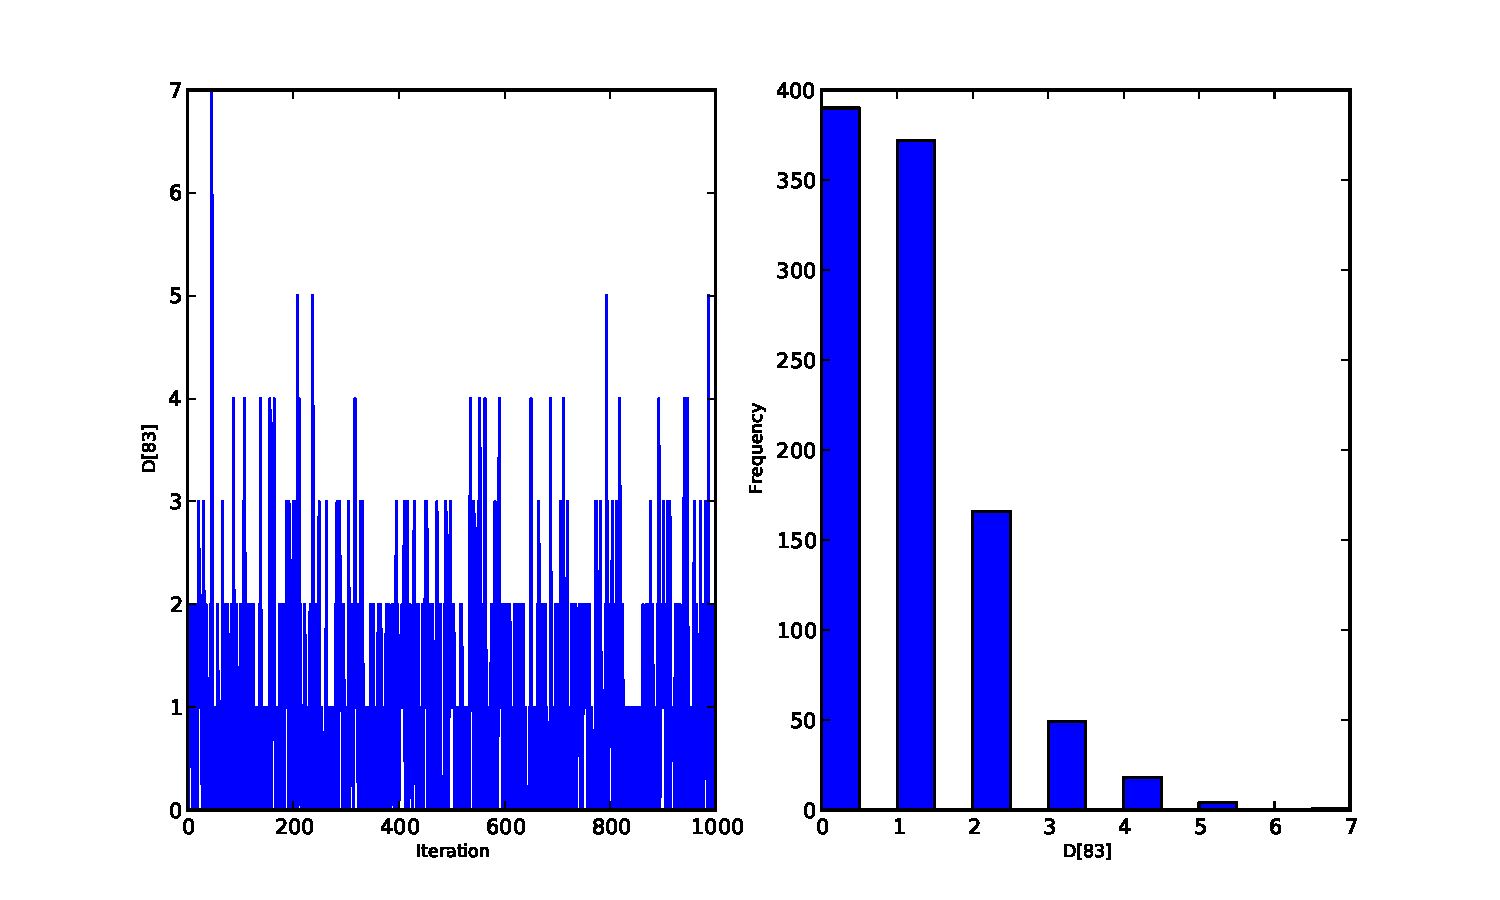
\includegraphics{missing.pdf}
\caption{Trace and posterior distribution of the missing data points in the example.}\end{figure}


\section{Fine-tuning the MCMC algorithm}
\label{tutorial:fine-tuning-the-mcmc-algorithm}
MCMC objects handle individual variables via \emph{step methods}, which determine how parameters are updated at each step of the MCMC algorithm. By default, step methods are automatically assigned to variables by PyMC. To see which step methods $M$ is using, look at its \code{step\_method\_dict} attribute with respect to each parameter:

\begin{Verbatim}[commandchars=\\\{\}]
\PYG{g+gp}{\textgreater{}\textgreater{}\textgreater{} }\PYG{n}{M}\PYG{o}{.}\PYG{n}{step\PYGZus{}method\PYGZus{}dict}\PYG{p}{[}\PYG{n}{disaster\PYGZus{}model}\PYG{o}{.}\PYG{n}{switchpoint}\PYG{p}{]}
\PYG{g+go}{[\textless{}pymc.StepMethods.DiscreteMetropolis object at 0x3e8cb50\textgreater{}]}

\PYG{g+gp}{\textgreater{}\textgreater{}\textgreater{} }\PYG{n}{M}\PYG{o}{.}\PYG{n}{step\PYGZus{}method\PYGZus{}dict}\PYG{p}{[}\PYG{n}{disaster\PYGZus{}model}\PYG{o}{.}\PYG{n}{early\PYGZus{}mean}\PYG{p}{]}
\PYG{g+go}{[\textless{}pymc.StepMethods.Metropolis object at 0x3e8cbb0\textgreater{}]}

\PYG{g+gp}{\textgreater{}\textgreater{}\textgreater{} }\PYG{n}{M}\PYG{o}{.}\PYG{n}{step\PYGZus{}method\PYGZus{}dict}\PYG{p}{[}\PYG{n}{disaster\PYGZus{}model}\PYG{o}{.}\PYG{n}{late\PYGZus{}mean}\PYG{p}{]}
\PYG{g+go}{[\textless{}pymc.StepMethods.Metropolis object at 0x3e8ccb0\textgreater{}]}
\end{Verbatim}

The value of \code{step\_method\_dict} corresponding to a particular variable is a list of the step methods $M$ is using to handle that variable.

You can force $M$ to use a particular step method by calling \code{M.use\_step\_method} before telling it to sample. The following call will cause $M$ to handle \code{late\_mean} with a standard \code{Metropolis} step method, but with proposal standard deviation equal to $2$:

\begin{Verbatim}[commandchars=\\\{\}]
\PYG{g+gp}{\textgreater{}\textgreater{}\textgreater{} }\PYG{k+kn}{from} \PYG{n+nn}{pymc} \PYG{k+kn}{import} \PYG{n}{Metropolis}
\PYG{g+gp}{\textgreater{}\textgreater{}\textgreater{} }\PYG{n}{M}\PYG{o}{.}\PYG{n}{use\PYGZus{}step\PYGZus{}method}\PYG{p}{(}\PYG{n}{Metropolis}\PYG{p}{,} \PYG{n}{disaster\PYGZus{}model}\PYG{o}{.}\PYG{n}{late\PYGZus{}mean}\PYG{p}{,} \PYG{n}{proposal\PYGZus{}sd}\PYG{o}{=}\PYG{l+m+mf}{2.}\PYG{p}{)}
\end{Verbatim}

Another step method class, \code{AdaptiveMetropolis}, is better at handling highly-correlated variables. If your model mixes poorly, using \code{AdaptiveMetropolis} is a sensible first thing to try.


\section{Beyond the basics}
\label{tutorial:beyond-the-basics}
That was a brief introduction to basic PyMC usage. Many more topics are covered in the subsequent sections, including:
\begin{itemize}
\item {} 
Class \code{Potential}, another building block for probability models in addition to \code{Stochastic} and \code{Deterministic}

\item {} 
Normal approximations

\item {} 
Using custom probability distributions

\item {} 
Object architecture

\item {} 
Saving traces to the disk, or streaming them to the disk during sampling

\item {} 
Writing your own step methods and fitting algorithms.

\end{itemize}

Also, be sure to check out the documentation for the Gaussian process extension, which is available on PyMC's \href{http://code.google.com/p/pymc/downloads/list}{download} page.


\chapter{Building models}
\label{modelbuilding:chap-modelbuilding}\label{modelbuilding:building-models}\label{modelbuilding::doc}
Bayesian inference begins with specification of a probability model relating unknown variables to data. PyMC provides three basic building blocks for Bayesian probability models: \code{Stochastic}, \code{Deterministic} and \code{Potential}.

A \code{Stochastic} object represents a variable whose value is not completely determined by its parents, and a \code{Deterministic} object represents a variable that is entirely determined by its parents. In object-oriented programming parlance, \code{Stochastic} and \code{Deterministic} are subclasses of the \code{Variable} class, which only serves as a template for other classes and is never actually implemented in models.

The third basic class, \code{Potential}, represents `factor potentials' ({\hyperref[references:lauritzen-1990]{{[}Lauritzen\_1990{]}}},{[}Jordan\_2004{]}\_), which are \emph{not} variables but simply terms and/or constraints that are multiplied into joint distributions to modify them. \code{Potential} and \code{Variable} are subclasses of \code{Node}.

PyMC probability models are simply linked groups of \code{Stochastic}, \code{Deterministic} and \code{Potential} objects. These objects have very limited awareness of the models in which they are embedded and do not themselves possess methods for updating their values in fitting algorithms. Objects responsible for fitting probability models are described in chapter {\hyperref[modelfitting:chap-modelfitting]{\emph{Fitting Models}}}.


\section{The Stochastic class}
\label{modelbuilding:stochastic}\label{modelbuilding:the-stochastic-class}
A stochastic variable has the following primary attributes:
\begin{description}
\item[{\code{value}:}] \leavevmode
The variable's current value.

\item[{\code{logp}:}] \leavevmode
The log-probability of the variable's current value given the values of its
parents.

\end{description}

A stochastic variable can optionally be endowed with a method called \code{random}, which draws a value for the variable given the values of its parents \footnote{
Note that the \code{random} method does not provide a Gibbs sample unless the
variable has no children.
}. Stochastic objects have the following additional attributes:
\begin{description}
\item[{\code{parents}:}] \leavevmode
A dictionary containing the variable's parents. The keys of the dictionary
correspond to the names assigned to the variable's parents by the variable,
and the values correspond to the actual parents. For example, the keys of
$s$`s parents dictionary in model (\eqref{modelbuilding-disastermodel}) would be
\code{'t\_l'} and \code{'t\_h'}. Thanks to Python's dynamic typing, the actual
parents (\emph{i.e.} the values of the dictionary) may be of any class or type.

\item[{\code{children}:}] \leavevmode
A set containing the variable's children.

\item[{\code{extended\_parents}:}] \leavevmode
A set containing all the stochastic variables on which the variable depends
either directly or via a sequence of deterministic variables. If the value
of any of these variables changes, the variable will need to recompute its
log-probability.

\item[{\code{extended\_children}:}] \leavevmode
A set containing all the stochastic variables and potentials that depend on
the variable either directly or via a sequence of deterministic variables.
If the variable's value changes, all of these variables will need to
recompute their log-probabilities.

\item[{\code{observed}:}] \leavevmode
A flag (boolean) indicating whether the variable's value has been observed
(is fixed).

\item[{\code{dtype}:}] \leavevmode
A NumPy dtype object (such as \code{numpy.int}) that specifies the type of the
variable's value to fitting methods. If this is \code{None} (default) then no
type is enforced.

\end{description}


\subsection{Creation of stochastic variables}
\label{modelbuilding:creation-of-stochastic-variables}
There are three main ways to create stochastic variables, called the
\textbf{automatic}, \textbf{decorator}, and \textbf{direct} interfaces.
\begin{description}
\item[{\textbf{Automatic}}] \leavevmode
Stochastic variables with standard distributions provided by PyMC (see
chapter {\hyperref[distributions:chap-distributions]{\emph{Probability distributions}}}) can be created in a single line using
special subclasses of \code{Stochastic}. For example, the
uniformly-distributed discrete variable $s$ in (\eqref{modelbuilding-disastermodel})
could be created using the automatic interface as follows:

\begin{Verbatim}[commandchars=\\\{\}]
\PYG{k+kn}{import} \PYG{n+nn}{pymc} \PYG{k+kn}{as} \PYG{n+nn}{pm}
\PYG{n}{s} \PYG{o}{=} \PYG{n}{pymc}\PYG{o}{.}\PYG{n}{DiscreteUniform}\PYG{p}{(}\PYG{l+s}{'}\PYG{l+s}{s}\PYG{l+s}{'}\PYG{p}{,} \PYG{l+m+mi}{1851}\PYG{p}{,} \PYG{l+m+mi}{1962}\PYG{p}{,} \PYG{n}{value}\PYG{o}{=}\PYG{l+m+mi}{1900}\PYG{p}{)}
\end{Verbatim}

In addition to the classes in chapter {\hyperref[distributions:chap-distributions]{\emph{Probability distributions}}},
\code{scipy.stats.distributions}` random variable classes are wrapped as
\code{Stochastic} subclasses if SciPy is installed. These distributions are in
the submodule \code{pymc.SciPyDistributions}.

Users can call the class factory \code{stochastic\_from\_dist} to produce
\code{Stochastic} subclasses of their own from probability distributions not
included with PyMC.

\item[{\textbf{Decorator}}] \leavevmode
Uniformly-distributed discrete stochastic variable $s$ in
(\eqref{modelbuilding-disastermodel}) could alternatively be created from a function that
computes its log-probability as follows:

\begin{Verbatim}[commandchars=\\\{\}]
\PYG{n+nd}{@pymc.stochastic}\PYG{p}{(}\PYG{n}{dtype}\PYG{o}{=}\PYG{n+nb}{int}\PYG{p}{)}
\PYG{k}{def} \PYG{n+nf}{s}\PYG{p}{(}\PYG{n}{value}\PYG{o}{=}\PYG{l+m+mi}{1900}\PYG{p}{,} \PYG{n}{t\PYGZus{}l}\PYG{o}{=}\PYG{l+m+mi}{1851}\PYG{p}{,} \PYG{n}{t\PYGZus{}h}\PYG{o}{=}\PYG{l+m+mi}{1962}\PYG{p}{)}\PYG{p}{:}
    \PYG{l+s+sd}{"""The switchpoint for the rate of disaster occurrence."""}
    \PYG{k}{if} \PYG{n}{value} \PYG{o}{\textgreater{}} \PYG{n}{t\PYGZus{}h} \PYG{o+ow}{or} \PYG{n}{value} \PYG{o}{\textless{}} \PYG{n}{t\PYGZus{}l}\PYG{p}{:}
        \PYG{c}{\PYGZsh{} Invalid values}
        \PYG{k}{return} \PYG{o}{-}\PYG{n}{numpy}\PYG{o}{.}\PYG{n}{inf}
    \PYG{k}{else}\PYG{p}{:}
        \PYG{c}{\PYGZsh{} Uniform log-likelihood}
        \PYG{k}{return} \PYG{o}{-}\PYG{n}{numpy}\PYG{o}{.}\PYG{n}{log}\PYG{p}{(}\PYG{n}{t\PYGZus{}h} \PYG{o}{-} \PYG{n}{t\PYGZus{}l} \PYG{o}{+} \PYG{l+m+mi}{1}\PYG{p}{)}
\end{Verbatim}

Note that this is a simple Python function preceded by a Python expression
called a \textbf{decorator} {\hyperref[references:vanrossum-2010]{{[}vanRossum\_2010{]}}}, here called \code{@stochastic}.
Generally, decorators enhance functions with additional properties or
functionality. The \code{Stochastic} object produced by the \code{@stochastic}
decorator will evaluate its log-probability using the function $s$.
The \code{value} argument, which is required, provides an initial value for
the variable. The remaining arguments will be assigned as parents of
$s$ (\emph{i.e.} they will populate the \code{parents} dictionary).

To emphasize, the Python function decorated by \code{@stochastic} should
compute the \emph{log}-density or \emph{log}-probability of the variable. That is why
the return value in the example above is $-\log(t_h-t_l+1)$ rather
than $1/(t_h-t_l+1)$.

The \code{value} and parents of stochastic variables may be any objects,
provided the log-probability function returns a real number (\code{float}).
PyMC and SciPy both provide implementations of several standard probability
distributions that may be helpful for creating custom stochastic variables.

The decorator stochastic can take any of the arguments
\code{Stochastic.\_\_init\_\_} takes except \code{parents}, \code{logp}, \code{random}, \code{doc} and \code{value}. These arguments include \code{trace}, \code{plot}, \code{verbose}, \code{dtype}, \code{rseed} and \code{name}.

The decorator interface has a slightly more complex implementation which
allows you to specify a \code{random} method for sampling the stochastic
variable's value conditional on its parents.

\begin{Verbatim}[commandchars=\\\{\}]
\PYG{n+nd}{@pymc.stochastic}\PYG{p}{(}\PYG{n}{dtype}\PYG{o}{=}\PYG{n+nb}{int}\PYG{p}{)}
\PYG{k}{def} \PYG{n+nf}{s}\PYG{p}{(}\PYG{n}{value}\PYG{o}{=}\PYG{l+m+mi}{1900}\PYG{p}{,} \PYG{n}{t\PYGZus{}l}\PYG{o}{=}\PYG{l+m+mi}{1851}\PYG{p}{,} \PYG{n}{t\PYGZus{}h}\PYG{o}{=}\PYG{l+m+mi}{1962}\PYG{p}{)}\PYG{p}{:}
    \PYG{l+s+sd}{"""The switchpoint for the rate of disaster occurrence."""}

    \PYG{k}{def} \PYG{n+nf}{logp}\PYG{p}{(}\PYG{n}{value}\PYG{p}{,} \PYG{n}{t\PYGZus{}l}\PYG{p}{,} \PYG{n}{t\PYGZus{}h}\PYG{p}{)}\PYG{p}{:}
        \PYG{k}{if} \PYG{n}{value} \PYG{o}{\textgreater{}} \PYG{n}{t\PYGZus{}h} \PYG{o+ow}{or} \PYG{n}{value} \PYG{o}{\textless{}} \PYG{n}{t\PYGZus{}l}\PYG{p}{:}
            \PYG{k}{return} \PYG{o}{-}\PYG{n}{numpy}\PYG{o}{.}\PYG{n}{inf}
        \PYG{k}{else}\PYG{p}{:}
            \PYG{k}{return} \PYG{o}{-}\PYG{n}{numpy}\PYG{o}{.}\PYG{n}{log}\PYG{p}{(}\PYG{n}{t\PYGZus{}h} \PYG{o}{-} \PYG{n}{t\PYGZus{}l} \PYG{o}{+} \PYG{l+m+mi}{1}\PYG{p}{)}

    \PYG{k}{def} \PYG{n+nf}{random}\PYG{p}{(}\PYG{n}{t\PYGZus{}l}\PYG{p}{,} \PYG{n}{t\PYGZus{}h}\PYG{p}{)}\PYG{p}{:}
        \PYG{k}{return} \PYG{n}{numpy}\PYG{o}{.}\PYG{n}{round}\PYG{p}{(} \PYG{p}{(}\PYG{n}{t\PYGZus{}l} \PYG{o}{-} \PYG{n}{t\PYGZus{}h}\PYG{p}{)} \PYG{o}{*} \PYG{n}{random}\PYG{p}{(}\PYG{p}{)} \PYG{p}{)} \PYG{o}{+} \PYG{n}{t\PYGZus{}l}
\end{Verbatim}

The stochastic variable again gets its name, docstring and parents from
function $s$, but in this case it will evaluate its log-probability
using the \code{logp} function. The \code{random} function will be used when
\code{s.random()} is called. Note that \code{random} doesn't take a \code{value}
argument, as it generates values itself.

\item[{\textbf{Direct}}] \leavevmode
It's possible to instantiate \code{Stochastic} directly:

\begin{Verbatim}[commandchars=\\\{\}]
\PYG{k}{def} \PYG{n+nf}{s\PYGZus{}logp}\PYG{p}{(}\PYG{n}{value}\PYG{p}{,} \PYG{n}{t\PYGZus{}l}\PYG{p}{,} \PYG{n}{t\PYGZus{}h}\PYG{p}{)}\PYG{p}{:}
    \PYG{k}{if} \PYG{n}{value} \PYG{o}{\textgreater{}} \PYG{n}{t\PYGZus{}h} \PYG{o+ow}{or} \PYG{n}{value} \PYG{o}{\textless{}} \PYG{n}{t\PYGZus{}l}\PYG{p}{:}
        \PYG{k}{return} \PYG{o}{-}\PYG{n}{numpy}\PYG{o}{.}\PYG{n}{inf}
    \PYG{k}{else}\PYG{p}{:}
        \PYG{k}{return} \PYG{o}{-}\PYG{n}{numpy}\PYG{o}{.}\PYG{n}{log}\PYG{p}{(}\PYG{n}{t\PYGZus{}h} \PYG{o}{-} \PYG{n}{t\PYGZus{}l} \PYG{o}{+} \PYG{l+m+mi}{1}\PYG{p}{)}

\PYG{k}{def} \PYG{n+nf}{s\PYGZus{}rand}\PYG{p}{(}\PYG{n}{t\PYGZus{}l}\PYG{p}{,} \PYG{n}{t\PYGZus{}h}\PYG{p}{)}\PYG{p}{:}
    \PYG{k}{return} \PYG{n}{numpy}\PYG{o}{.}\PYG{n}{round}\PYG{p}{(} \PYG{p}{(}\PYG{n}{t\PYGZus{}l} \PYG{o}{-} \PYG{n}{t\PYGZus{}h}\PYG{p}{)} \PYG{o}{*} \PYG{n}{random}\PYG{p}{(}\PYG{p}{)} \PYG{p}{)} \PYG{o}{+} \PYG{n}{t\PYGZus{}l}

\PYG{n}{s} \PYG{o}{=} \PYG{n}{Stochastic}\PYG{p}{(} \PYG{n}{logp} \PYG{o}{=} \PYG{n}{s\PYGZus{}logp}\PYG{p}{,}
                \PYG{n}{doc} \PYG{o}{=} \PYG{l+s}{'}\PYG{l+s}{The switchpoint for the rate of disaster occurrence.}\PYG{l+s}{'}\PYG{p}{,}
                \PYG{n}{name} \PYG{o}{=} \PYG{l+s}{'}\PYG{l+s}{s}\PYG{l+s}{'}\PYG{p}{,}
                \PYG{n}{parents} \PYG{o}{=} \PYG{p}{\PYGZob{}}\PYG{l+s}{'}\PYG{l+s}{t\PYGZus{}l}\PYG{l+s}{'}\PYG{p}{:} \PYG{l+m+mi}{1851}\PYG{p}{,} \PYG{l+s}{'}\PYG{l+s}{t\PYGZus{}h}\PYG{l+s}{'}\PYG{p}{:} \PYG{l+m+mi}{1962}\PYG{p}{\PYGZcb{}}\PYG{p}{,}
                \PYG{n}{random} \PYG{o}{=} \PYG{n}{s\PYGZus{}rand}\PYG{p}{,}
                \PYG{n}{trace} \PYG{o}{=} \PYG{n+nb+bp}{True}\PYG{p}{,}
                \PYG{n}{value} \PYG{o}{=} \PYG{l+m+mi}{1900}\PYG{p}{,}
                \PYG{n}{dtype}\PYG{o}{=}\PYG{n+nb}{int}\PYG{p}{,}
                \PYG{n}{rseed} \PYG{o}{=} \PYG{l+m+mf}{1.}\PYG{p}{,}
                \PYG{n}{observed} \PYG{o}{=} \PYG{n+nb+bp}{False}\PYG{p}{,}
                \PYG{n}{cache\PYGZus{}depth} \PYG{o}{=} \PYG{l+m+mi}{2}\PYG{p}{,}
                \PYG{n}{plot}\PYG{o}{=}\PYG{n+nb+bp}{True}\PYG{p}{,}
                \PYG{n}{verbose} \PYG{o}{=} \PYG{l+m+mi}{0}\PYG{p}{)}
\end{Verbatim}

Notice that the log-probability and random variate functions are specified
externally and passed to \code{Stochastic} as arguments. This is a rather
awkward way to instantiate a stochastic variable; consequently, such
implementations should be rare.

\end{description}


\section{A Warning: Don't update stochastic variables' values in-place}
\label{modelbuilding:warning}\label{modelbuilding:a-warning-don-t-update-stochastic-variables-values-in-place}
\code{Stochastic} objects' values should not be updated in-place. This
confuses PyMC's caching scheme and corrupts the process used for
accepting or rejecting proposed values in the MCMC algorithm. The only
way a stochastic variable's value should be updated is using
statements of the following form:

\begin{Verbatim}[commandchars=\\\{\}]
\PYG{n}{A}\PYG{o}{.}\PYG{n}{value} \PYG{o}{=} \PYG{n}{new\PYGZus{}value}
\end{Verbatim}

The following are in-place updates and should \_never\_ be used:

\begin{Verbatim}[commandchars=@\[\]]
* []`[]`A.value += 3[]`[]`
* []`[]`A.value@PYGZlb[]2,1@PYGZrb[] = 5[]`[]`
* []`[]`A.value.attribute = new@_attribute@_value[]`[]`
\end{Verbatim}

This restriction becomes onerous if a step method proposes values for
the elements of an array-valued variable separately. In this case, it
may be preferable to partition the variable into several scalar-valued
variables stored in an array or list.


\section{Data}
\label{modelbuilding:id4}\label{modelbuilding:data}
Data are represented by \code{Stochastic} objects whose \code{observed} attribute is set to \code{True}. If a stochastic variable's \code{observed} flag is \code{True}, its value cannot be changed, and it won't be sampled by the fitting method.


\subsection{Declaring stochastic variables to be data}
\label{modelbuilding:declaring-stochastic-variables-to-be-data}
In each interface, an optional keyword argument \code{observed} can be set to \code{True}. In the decorator interface, this argument is added to the \code{@stochastic} decorator:

\begin{Verbatim}[commandchars=@\[\]]
@PYGZat[]pymc.stochastic(observed=True)
\end{Verbatim}

In the other interfaces, the \code{observed=True} argument is added to the instantiation of the \code{Stochastic}, or its subclass:

\begin{Verbatim}[commandchars=\\\{\}]
\PYG{n}{x} \PYG{o}{=} \PYG{n}{pymc}\PYG{o}{.}\PYG{n}{Binomial}\PYG{p}{(}\PYG{l+s}{'}\PYG{l+s}{x}\PYG{l+s}{'}\PYG{p}{,} \PYG{n}{n}\PYG{o}{=}\PYG{n}{n}\PYG{p}{,} \PYG{n}{p}\PYG{o}{=}\PYG{n}{p}\PYG{p}{,} \PYG{n}{observed}\PYG{o}{=}\PYG{n+nb+bp}{True}\PYG{p}{)}
\end{Verbatim}

Alternatively, in the decorator interface only, a \code{Stochastic} object's \code{observed} flag can be set to true by stacking an \code{@observed} decorator on top of the \code{@stochastic} decorator:

\begin{Verbatim}[commandchars=@\[\]]
@PYGZat[]pymc.observed(dtype=int)
     def ...
\end{Verbatim}


\section{The Deterministic class}
\label{modelbuilding:deterministic}\label{modelbuilding:the-deterministic-class}
The \code{Deterministic} class represents variables whose values are completely determined by the values of their parents. For example, in model (\eqref{modelbuilding-disastermodel}), $r$ is a \code{deterministic} variable. Recall it was defined by
\begin{eqnarray*}
    r_t=\left\{\begin{array}{ll}
        e & t\le s\\ l & t>s
        \end{array}\right.,
\end{eqnarray*}
so $r$`s value can be computed exactly from the values of its parents $e$, $l$ and $s$.

A \code{deterministic} variable's most important attribute is \code{value}, which gives the current value of the variable given the values of its parents. Like \code{Stochastic}`s \code{logp} attribute, this attribute is computed on-demand and cached for efficiency.

A Deterministic variable has the following additional attributes:
\begin{description}
\item[{\code{parents}:}] \leavevmode
A dictionary containing the variable's parents. The keys of the dictionary
correspond to the names assigned to the variable's parents by the variable,
\begin{quote}

and the values correspond to the actual parents.
\end{quote}

\item[{\code{children}:}] \leavevmode
A set containing the variable's children, which must be nodes.

\end{description}

Deterministic variables have no methods.


\subsection{Creation of deterministic variables}
\label{modelbuilding:creation-of-deterministic-variables}
Deterministic variables are less complicated than stochastic variables, and have similar \textbf{automatic}, \textbf{decorator}, and \textbf{direct} interfaces:
\begin{description}
\item[{\textbf{Automatic}}] \leavevmode\begin{description}
\item[{A handful of common functions have been wrapped in Deterministic objects.}] \leavevmode
These are brief enough to list:

\item[{\code{LinearCombination}:}] \leavevmode
Has two parents $x$ and $y$, both of which must be iterable (\emph{i.e.}
vector-valued). This function returns:

\item[{\code{Index}:}] \leavevmode\begin{description}
\item[{Has two parents $x$ and \code{index}. $x$ must be iterables,}] \leavevmode
\code{index} must be valued as an integer. The value of an \code{index} is:

\code{Index} is useful for implementing dynamic models, in which the
parent-child connections change.

\end{description}

\item[{\code{Lambda}:}] \leavevmode\begin{description}
\item[{Converts an anonymous function (in Python, called \textbf{lambda functions})}] \leavevmode
to a \code{Deterministic} instance on a single line.

\end{description}

\item[{\code{CompletedDirichlet}:}] \leavevmode\begin{description}
\item[{PyMC represents Dirichlet variables of length $k$ by the first}] \leavevmode
$k-1$ elements; since they must sum to 1, the $k^{th}$
element is determined by the others. \code{CompletedDirichlet} appends the
$k^{th}$ element to the value of its parent $D$.

\end{description}

\item[{\code{Logit}, \code{InvLogit}, \code{StukelLogit}, \code{StukelInvLogit}:}] \leavevmode
Common link functions for generalized linear models, and their inverses.

\item[{It’s a good idea to use these classes when feasible in order to give hints}] \leavevmode
to step methods.

\end{description}

\item[{\textbf{Elementary operations on variables}}] \leavevmode
Certain elementary operations on variables create deterministic variables.
For example:

\begin{Verbatim}[commandchars=\\\{\}]
\PYG{g+gp}{\textgreater{}\textgreater{}\textgreater{} }\PYG{n}{x} \PYG{o}{=} \PYG{n}{pymc}\PYG{o}{.}\PYG{n}{MvNormalCov}\PYG{p}{(}\PYG{l+s}{'}\PYG{l+s}{x}\PYG{l+s}{'}\PYG{p}{,}\PYG{n}{numpy}\PYG{o}{.}\PYG{n}{ones}\PYG{p}{(}\PYG{l+m+mi}{3}\PYG{p}{)}\PYG{p}{,}\PYG{n}{numpy}\PYG{o}{.}\PYG{n}{eye}\PYG{p}{(}\PYG{l+m+mi}{3}\PYG{p}{)}\PYG{p}{)}
\PYG{g+gp}{\textgreater{}\textgreater{}\textgreater{} }\PYG{n}{y} \PYG{o}{=} \PYG{n}{pymc}\PYG{o}{.}\PYG{n}{MvNormalCov}\PYG{p}{(}\PYG{l+s}{'}\PYG{l+s}{y}\PYG{l+s}{'}\PYG{p}{,}\PYG{n}{numpy}\PYG{o}{.}\PYG{n}{ones}\PYG{p}{(}\PYG{l+m+mi}{3}\PYG{p}{)}\PYG{p}{,}\PYG{n}{numpy}\PYG{o}{.}\PYG{n}{eye}\PYG{p}{(}\PYG{l+m+mi}{3}\PYG{p}{)}\PYG{p}{)}
\PYG{g+gp}{\textgreater{}\textgreater{}\textgreater{} }\PYG{k}{print} \PYG{n}{x}\PYG{o}{+}\PYG{n}{y}
\PYG{g+go}{\textless{}pymc.PyMCObjects.Deterministic '(x\PYGZus{}add\PYGZus{}y)' at 0x105c3bd10\textgreater{}}
\PYG{g+gp}{\textgreater{}\textgreater{}\textgreater{} }\PYG{k}{print} \PYG{n}{x}\PYG{p}{[}\PYG{l+m+mi}{0}\PYG{p}{]}
\PYG{g+go}{\textless{}pymc.CommonDeterministics.Index 'x[0]' at 0x105c52390\textgreater{}}
\PYG{g+gp}{\textgreater{}\textgreater{}\textgreater{} }\PYG{k}{print} \PYG{n}{x}\PYG{p}{[}\PYG{l+m+mi}{1}\PYG{p}{]}\PYG{o}{+}\PYG{n}{y}\PYG{p}{[}\PYG{l+m+mi}{2}\PYG{p}{]}
\PYG{g+go}{\textless{}pymc.PyMCObjects.Deterministic '(x[1]\PYGZus{}add\PYGZus{}y[2])' at 0x105c52410\textgreater{}}
\end{Verbatim}

All the objects thus created have \code{trace=False} and \code{plot=False} by
default. This conve- nient method of generating simple deterministics was
inspired by {\hyperref[references:kerman-2004]{{[}Kerman\_2004{]}}}.

\item[{\textbf{Decorator}}] \leavevmode
A deterministic variable can be created via a decorator in a way very similar to
\code{Stochastic}`s decorator interface:

\begin{Verbatim}[commandchars=\\\{\}]
\PYG{n+nd}{@pymc.deterministic}
\PYG{k}{def} \PYG{n+nf}{r}\PYG{p}{(}\PYG{n}{switchpoint} \PYG{o}{=} \PYG{n}{s}\PYG{p}{,} \PYG{n}{early\PYGZus{}rate} \PYG{o}{=} \PYG{n}{e}\PYG{p}{,} \PYG{n}{late\PYGZus{}rate} \PYG{o}{=} \PYG{n}{l}\PYG{p}{)}\PYG{p}{:}
    \PYG{l+s+sd}{"""The rate of disaster occurrence."""}
    \PYG{n}{value} \PYG{o}{=} \PYG{n}{zeros}\PYG{p}{(}\PYG{n}{N}\PYG{p}{)}
    \PYG{n}{value}\PYG{p}{[}\PYG{p}{:}\PYG{n}{switchpoint}\PYG{p}{]} \PYG{o}{=} \PYG{n}{early\PYGZus{}rate}
    \PYG{n}{value}\PYG{p}{[}\PYG{n}{switchpoint}\PYG{p}{:}\PYG{p}{]} \PYG{o}{=} \PYG{n}{late\PYGZus{}rate}
    \PYG{k}{return} \PYG{n}{value}
\end{Verbatim}

Notice that rather than returning the log-probability, as is the case for
\code{Stochastic} objects, the function returns the value of the deterministic
object, given its parents. This return value may be of any type, as is
\begin{quote}

suitable for the problem at hand. Also notice that, unlike for
\code{Stochastic} objects, there is no \code{value} argument passed, since the
value is calculated deterministically by the function itself. Arguments'
keys and values are converted into a parent dictionary as with
\code{Stochastic}`s short interface. The \code{deterministic} decorator can take
\code{trace}, \code{verbose} and \code{plot} arguments, like the \code{stochastic}
decorator \footnote{
Note that deterministic variables have no \code{observed} flag. If a deterministic
variable's value were known, its parents would be restricted to the inverse
image of that value under the deterministic variable's evaluation function. This
usage would be extremely difficult to support in general, but it can be
implemented for particular applications at the \code{StepMethod} level.
}.
\end{quote}

\item[{\textbf{Direct}}] \leavevmode
\code{Deterministic} objects can also be instantiated directly:

\begin{Verbatim}[commandchars=@\[\]]
def r@_eval(switchpoint = s, early@_rate = e, late@_rate = l):
    value = zeros(N)
    value@PYGZlb[]:switchpoint@PYGZrb[] = early@_rate
    value@PYGZlb[]switchpoint:@PYGZrb[] = late@_rate
    return value

r = pymc.Deterministic(  eval = r@_eval,
                    name = 'r',
                    parents = {'switchpoint': s, 'early@_rate': e, 'late@_rate': l}),
                    doc = 'The rate of disaster occurrence.',
                    trace = True,
                    verbose = 0,
                    dtype=float,
                    plot=False,
                    cache@_depth = 2)
\end{Verbatim}

\end{description}


\section{Containers}
\label{modelbuilding:containers}
In some situations it would be inconvenient to assign a unique label to each
parent of some variable. Consider $y$ in the following model:
\begin{align*}
    x_0 &\sim N (0,\tau_x)\\
    x_{i+1}|x_i &\sim \text{N}(x_i, \tau_x)\\
    &&i=0,\ldots, N-2\\
    y|x &\sim N \left(\sum_{i=0}^{N-1}x_i^2,\tau_y\right)
\end{align*}
Here, $y$ depends on every element of the Markov chain $x$, but we
wouldn't want to manually enter $N$ parent labels \code{{}`x\_0'}, \code{{}`x\_1'},
etc.

This situation can be handled naturally in PyMC:

\begin{Verbatim}[commandchars=@\[\]]
     N = 10
x@_0 = pymc.Normal([]`x@_0', mu=0, tau=1)

x = numpy.empty(N, dtype=object)
x@PYGZlb[]0@PYGZrb[] = x@_0

for i in range(1, N):

   xi = pymc.Normal([]`x@_@%i' @% i, mu=x@PYGZlb[]i-1@PYGZrb[], tau=1)

@PYGZat[]pymc.observed
def y(value=1, mu=x, tau=100):
    return pymc.normal@_like(value, numpy.sum(mu**2), tau)
\end{Verbatim}

PyMC automatically wraps array $x$ in an appropriate \code{Container} class. The expression \code{'x\_\%i' \% i} labels each \code{Normal} object in the container with the appropriate index $i$; so if \code{i=1}, the name of the
corresponding element becomes \code{{}`x\_1'}.

Containers, like variables, have an attribute called \code{value}. This attribute returns a copy of the (possibly nested) iterable that was passed into the container function, but with each variable inside replaced with its corresponding value.

Containers can currently be constructed from lists, tuples, dictionaries, Numpy arrays, modules, sets or any object with a \code{\_\_dict\_\_} attribute. Variables and non-variables can be freely mixed in these containers, and different types of containers can be nested \footnote{
Nodes whose parents are containers make private shallow copies of those
containers. This is done for technical reasons rather than to protect users from
accidental misuse.
}. Containers attempt to behave like the objects they wrap. All containers are subclasses of \code{ContainerBase}.

Containers have the following useful attributes in addition to \code{value}:
\begin{itemize}
\item {} 
\code{variables}

\item {} 
\code{stochastics}

\item {} 
\code{potentials}

\item {} 
\code{deterministics}

\item {} 
\code{data\_stochastics}

\item {} 
\code{step\_methods}.

\end{itemize}

Each of these attributes is a set containing all the objects of each type in a
container, and within any containers in the container.


\section{The Potential class}
\label{modelbuilding:potential}\label{modelbuilding:the-potential-class}
The joint density corresponding to model (\eqref{modelbuilding-disastermodel}) can be written
as follows:
\begin{eqnarray*}
    p(D,s,l,e) = p(D|s,l,e) p(s) p(l) p(e).
\end{eqnarray*}
Each factor in the joint distribution is a proper, normalized probability distribution for one of the variables conditional on its parents. Such factors are contributed by \code{Stochastic} objects.

In some cases, it's nice to be able to modify the joint density by incorporating terms that don't correspond to probabilities of variables conditional on parents, for example:
\begin{eqnarray*}
    p(x_0, x_2, \ldots x_{N-1}) \propto \prod_{i=0}^{N-2} \psi_i(x_i, x_{i+1}).
\end{eqnarray*}
In other cases we may want to add probability terms to existing models. For example, suppose we want to constrain the difference between $e$ and $l$ in (\eqref{modelbuilding-disastermodel}) to be less than 1, so that the joint density becomes
\begin{eqnarray*}
    p(D,s,l,e) \propto p(D|s,l,e) p(s) p(l) p(e) I(|e-l|<1).
\end{eqnarray*}
Its possible to express this constraint by adding variables to the model, or by grouping $e$ and $l$ to form a vector-valued variable, but it's uncomfortable to do so.

Arbitrary factors such as $\psi$ and the indicator function $I(|e-l|<1)$ are implemented by objects of class \code{Potential} ({\hyperref[references:lauritzen-1990]{{[}Lauritzen\_1990{]}}} and {\hyperref[references:jordan-2004]{{[}Jordan\_2004{]}}} call these terms `factor potentials'). Bayesian hierarchical notation (cf model (\eqref{modelbuilding-disastermodel})) doesn't accomodate these potentials. They are often used in cases where there is no natural dependence hierarchy, such as the first example above (which is known as a Markov random field). They are also useful for expressing `soft data' {\hyperref[references:christakos-2002]{{[}Christakos\_2002{]}}} as in the second example below.

Potentials have one important attribute, \code{logp}, the log of their current probability or probability density value given the values of their parents. The only other additional attribute of interest is \code{parents}, a dictionary containing the potential's parents. Potentials have no methods. They have no \code{trace} attribute, because they are not variables. They cannot serve as parents of variables (for the same reason), so they have no \code{children} attribute.


\subsection{An example of soft data}
\label{modelbuilding:an-example-of-soft-data}
The role of potentials can be confusing, so we will provide another example: we have a dataset $t$ consisting of the days on which several marked animals were recaptured. We believe that the probability $S$ that an animal is not recaptured on any given day can be explained by a covariate vector $x$. We model this situation as follows:
\begin{eqnarray*}
    t_i|S_i \sim \text{Geometric}(S_i), & i=1\ldots N\\
    S_i = \text{logit}^{-1}(\beta x_i), &i=1\ldots N\\
    \beta\sim \text{N}(\mu_\beta, V_\beta).
\end{eqnarray*}
So far, so good. Now suppose we have some knowledge of other related experiments and we have a good idea of what $S$ will be independent of the value of $\beta$. It's not obvious how to work this `soft data', because as we've written the model $S$ is completely determined by $\beta$. There are three options within the strict Bayesian hierarchical framework:
\begin{itemize}
\item {} 
Work the soft data into the prior on $\beta$.

\item {} 
Incorporate the data from the previous experiments explicitly into the model.

\item {} 
Refactor the model so that $S$ is at the bottom of the hierarchy, and
assign the prior directly.

\end{itemize}

Factor potentials provide a convenient way to incorporate the soft data without the need for such major modifications. We can simply modify the joint distribution from
\begin{eqnarray*}
    p(t|S(x,\beta)) p(\beta)
\end{eqnarray*}
to
\begin{eqnarray*}
    \gamma(S) p(t|S(x,\beta)) p(\beta),
\end{eqnarray*}
where the value of $\gamma$ is large if $S$`s value is plausible (based on our external information) and small otherwise. We do not know the normalizing constant for the new distribution, but we don't need it to use most popular fitting algorithms. It's a good idea to check the induced priors on $S$ and $\beta$ for sanity. This can be done in PyMC by fitting the model with the data $t$ removed.

Its important to understand that $\gamma$ is not a variable, so it does not have a value. That means, among other things, there will be no $\gamma$ column in MCMC traces.


\subsection{Creation of Potentials}
\label{modelbuilding:creation-of-potentials}
There are two ways to create potentials:
\begin{description}
\item[{\textbf{Decorator}}] \leavevmode
A potential can be created via a decorator in a way very similar to
\code{Deterministic}`s decorator interface:

\begin{Verbatim}[commandchars=\\\{\}]
\PYG{n+nd}{@pymc.potential}
\PYG{k}{def} \PYG{n+nf}{psi\PYGZus{}i}\PYG{p}{(}\PYG{n}{x\PYGZus{}lo} \PYG{o}{=} \PYG{n}{x}\PYG{p}{[}\PYG{n}{i}\PYG{p}{]}\PYG{p}{,} \PYG{n}{x\PYGZus{}hi} \PYG{o}{=} \PYG{n}{x}\PYG{p}{[}\PYG{n}{i}\PYG{o}{+}\PYG{l+m+mi}{1}\PYG{p}{]}\PYG{p}{)}\PYG{p}{:}
    \PYG{l+s+sd}{"""A pair potential"""}
    \PYG{k}{return} \PYG{o}{-}\PYG{p}{(}\PYG{n}{xlo} \PYG{o}{-} \PYG{n}{xhi}\PYG{p}{)}\PYG{o}{*}\PYG{o}{*}\PYG{l+m+mi}{2}
\end{Verbatim}
\begin{description}
\item[{The function supplied should return the potential's current}] \leavevmode
\emph{log}-probability or \emph{log}-density as a Numpy \code{float}. The \code{potential}
decorator can take \code{verbose} and \code{cache\_depth} arguments like the
\code{stochastic} decorator.

\end{description}

\item[{\textbf{Direct}}] \leavevmode
The same potential could be created directly as follows:

\begin{Verbatim}[commandchars=\\\{\}]
\PYG{k}{def} \PYG{n+nf}{psi\PYGZus{}i\PYGZus{}logp}\PYG{p}{(}\PYG{n}{x\PYGZus{}lo} \PYG{o}{=} \PYG{n}{x}\PYG{p}{[}\PYG{n}{i}\PYG{p}{]}\PYG{p}{,} \PYG{n}{x\PYGZus{}hi} \PYG{o}{=} \PYG{n}{x}\PYG{p}{[}\PYG{n}{i}\PYG{o}{+}\PYG{l+m+mi}{1}\PYG{p}{]}\PYG{p}{)}\PYG{p}{:}
    \PYG{k}{return} \PYG{o}{-}\PYG{p}{(}\PYG{n}{xlo} \PYG{o}{-} \PYG{n}{xhi}\PYG{p}{)}\PYG{o}{*}\PYG{o}{*}\PYG{l+m+mi}{2}

\PYG{n}{psi\PYGZus{}i} \PYG{o}{=} \PYG{n}{pymc}\PYG{o}{.}\PYG{n}{Potential}\PYG{p}{(}  \PYG{n}{logp} \PYG{o}{=} \PYG{n}{psi\PYGZus{}i\PYGZus{}logp}\PYG{p}{,}
                    \PYG{n}{name} \PYG{o}{=} \PYG{l+s}{'}\PYG{l+s}{psi\PYGZus{}i}\PYG{l+s}{'}\PYG{p}{,}
                    \PYG{n}{parents} \PYG{o}{=} \PYG{p}{\PYGZob{}}\PYG{l+s}{'}\PYG{l+s}{xlo}\PYG{l+s}{'}\PYG{p}{:} \PYG{n}{x}\PYG{p}{[}\PYG{n}{i}\PYG{p}{]}\PYG{p}{,} \PYG{l+s}{'}\PYG{l+s}{xhi}\PYG{l+s}{'}\PYG{p}{:} \PYG{n}{x}\PYG{p}{[}\PYG{n}{i}\PYG{o}{+}\PYG{l+m+mi}{1}\PYG{p}{]}\PYG{p}{\PYGZcb{}}\PYG{p}{,}
                    \PYG{n}{doc} \PYG{o}{=} \PYG{l+s}{'}\PYG{l+s}{A pair potential}\PYG{l+s}{'}\PYG{p}{,}
                    \PYG{n}{verbose} \PYG{o}{=} \PYG{l+m+mi}{0}\PYG{p}{,}
                    \PYG{n}{cache\PYGZus{}depth} \PYG{o}{=} \PYG{l+m+mi}{2}\PYG{p}{)}
\end{Verbatim}

\end{description}


\section{Graphing models}
\label{modelbuilding:graphical}\label{modelbuilding:graphing-models}
The function \code{dag} (or \code{graph}) in \code{pymc.graph} draws graphical representations of \code{Model} (Chapter {\hyperref[modelfitting:chap-modelfitting]{\emph{Fitting Models}}}) instances using \textbf{GraphViz} via the Python package \textbf{PyDot}. See {\hyperref[references:lauritzen-1990]{{[}Lauritzen\_1990{]}}} and {\hyperref[references:jordan-2004]{{[}Jordan\_2004{]}}} for more discussion of useful information that can be read off of graphical models. Note that these authors do not consider deterministic variables.

The symbol for stochastic variables is an ellipse. Parent-child relationships are indicated by arrows. These arrows point from parent to child and are labeled with the names assigned to the parents by the children. PyMC's symbol for deterministic variables is a downward-pointing triangle. A graphical representation of model \eqref{modelbuilding-disastermodel} is shown in {\hyperref[tutorial:dag]{\emph{Directed acyclic graph of the relationships in the coal mining disaster model example.}}}. Note that  $D$ is shaded because it is flagged as data.

The symbol for factor potentials is a rectangle, as in the following model.
Factor potentials are usually associated with \emph{undirected} grahical models. In
undirected representations, each parent of a potential is connected to every
other parent by an undirected edge. The undirected representation of the model
pictured above is much more compact: Directed or mixed graphical models can be
represented in an undirected form by `moralizing', which is done by the function \code{pymc.graph.moral\_graph}.
\begin{figure}[htbp]
\centering
\capstart

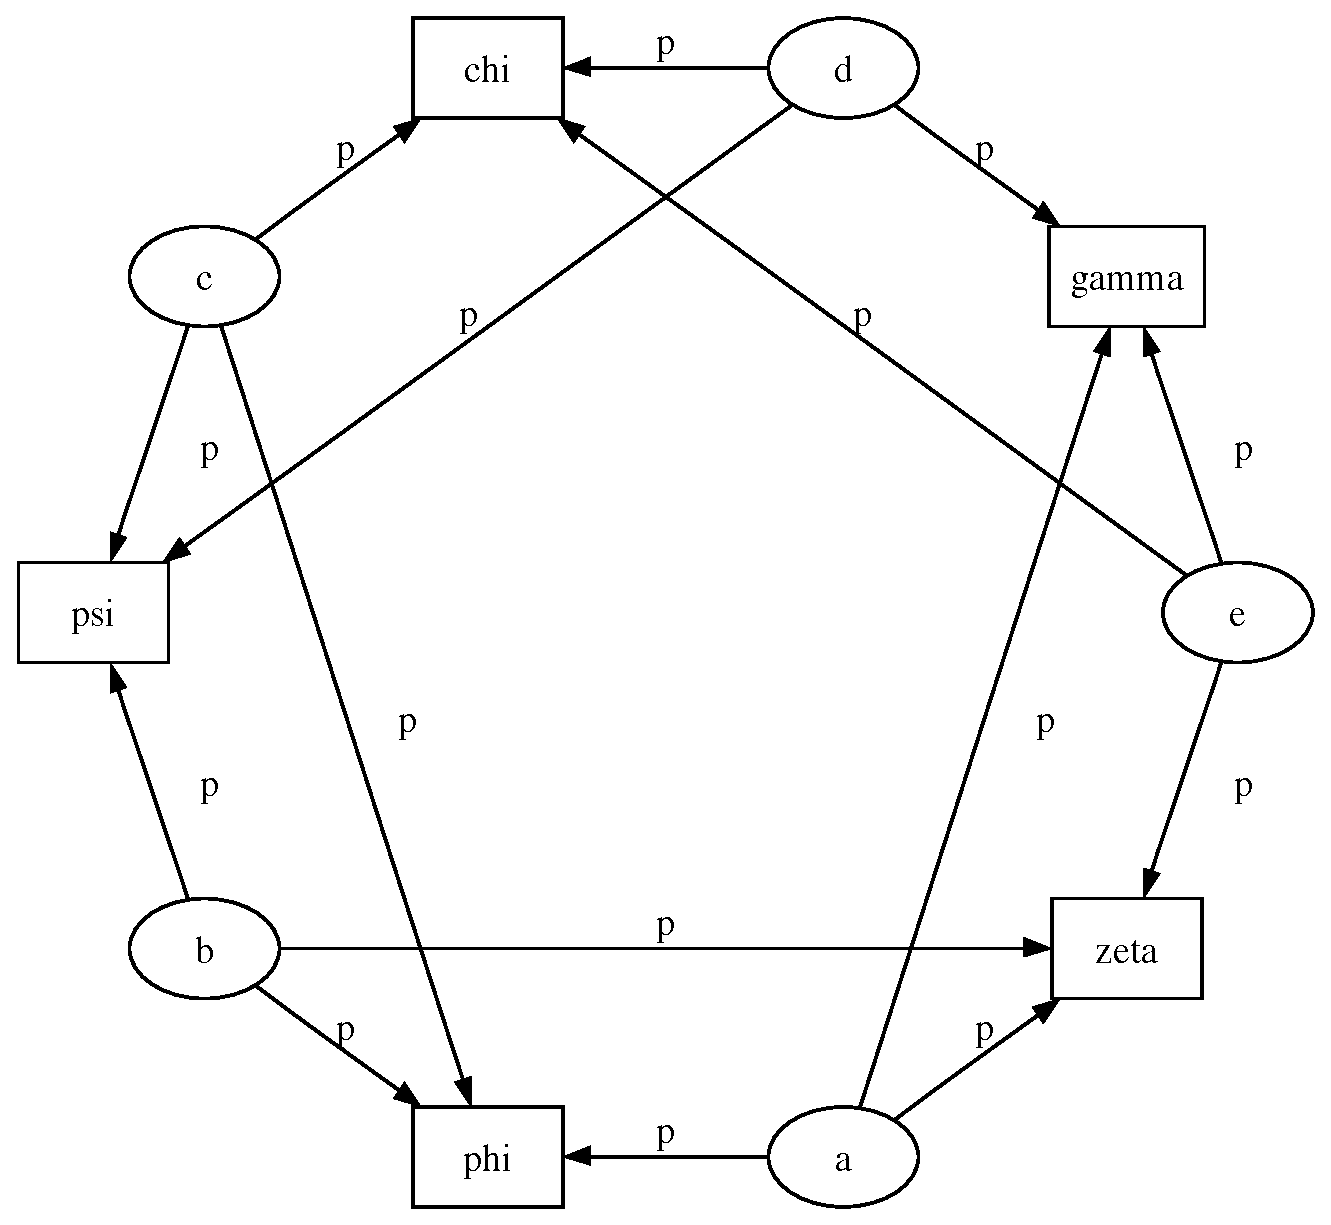
\includegraphics{PotExample.pdf}
\caption{Directed graphical model example. Factor potentials are represented by rectangles and stochastic variables by ellipses.}\label{modelbuilding:pot}\end{figure}


\section{Class LazyFunction and caching}
\label{modelbuilding:class-lazyfunction-and-caching}\label{modelbuilding:sec-caching}
This section gives an overview of how PyMC computes log-probabilities. This is advanced information that is not required in order to use PyMC.

The \code{logp} attributes of stochastic variables and potentials and the \code{value} attributes of deterministic variables are wrappers for instances of class \code{LazyFunction}. Lazy functions are wrappers for ordinary Python functions. A lazy function \code{L} could be created from a function \code{fun} as follows:

\begin{Verbatim}[commandchars=\\\{\}]
\PYG{n}{L} \PYG{o}{=} \PYG{n}{pymc}\PYG{o}{.}\PYG{n}{LazyFunction}\PYG{p}{(}\PYG{n}{fun}\PYG{p}{,} \PYG{n}{arguments}\PYG{p}{)}
\end{Verbatim}

The argument \code{arguments} is a dictionary container; \code{fun} must accept keyword arguments only. When \code{L}`s \code{get()} method is called, the return value is the same as the call

\begin{Verbatim}[commandchars=\\\{\}]
\PYG{n}{fun}\PYG{p}{(}\PYG{o}{*}\PYG{o}{*}\PYG{n}{arguments}\PYG{o}{.}\PYG{n}{value}\PYG{p}{)}
\end{Verbatim}

Note that no arguments need to be passed to \code{L.get}; lazy functions memorize their arguments.

Before calling \code{fun}, \code{L} will check the values of \code{arguments.variables} against an internal cache. This comparison is done \emph{by reference}, not by value, and this is part of the reason why stochastic variables' values cannot be updated in-place. If \code{arguments.variables}` values match a frame of the cache, the corresponding output value is returned and \code{fun} is not called. If a call to \code{fun} is needed, \code{arguments.variables}` values and the return value replace the oldest frame in the cache. The depth of the cache can be set using the optional init argument \code{cache\_depth}, which defaults to 2.

Caching is helpful in MCMC, because variables' log-probabilities and values tend to be queried multiple times for the same parental value configuration. The default cache depth of 2 turns out to be most useful in Metropolis-Hastings-type algorithms involving proposed values that may be rejected.

Lazy functions are implemented in C using Pyrex, a language for writing Python extensions.


\chapter{Fitting Models}
\label{modelfitting:chap-modelfitting}\label{modelfitting::doc}\label{modelfitting:fitting-models}
PyMC provides three objects that fit models:
\begin{itemize}
\item {} 
\code{MCMC}, which coordinates Markov chain Monte Carlo algorithms. The actual work of updating stochastic variables conditional on the rest of the model is done by \code{StepMethod} objects, which are described in this chapter.

\item {} 
\code{MAP}, which computes maximum \emph{a posteriori} estimates.

\item {} 
\code{NormApprox}, which computes the `normal approximation' {\hyperref[references:gelman-2004]{{[}Gelman\_2004{]}}}: the joint distribution of all stochastic variables in a model is approximated as normal using local information at the maximum \emph{a posteriori} estimate.

\end{itemize}

All three objects are subclasses of \code{Model}, which is PyMC's base class for fitting methods. \code{MCMC} and \code{NormApprox}, both of which can produce samples from the posterior, are subclasses of \code{Sampler}, which is PyMC's base class for Monte Carlo fitting methods. \code{Sampler} provides a generic sampling loop method and database support for storing large sets of joint samples. These base classes implement some basic methods that are inherited by the three implemented fitting methods, so they are documented at the end of this section.


\section{Creating models}
\label{modelfitting:sec-modelinstantiation}\label{modelfitting:creating-models}
The first argument to any fitting method's \code{\_\_init\_\_} method, including that of \code{MCMC}, is called \code{input}. The \code{input} argument can be just about anything; once you have defined the nodes that make up your model, you shouldn't even have to think about how to wrap them in a \code{Model} instance. Some examples of model instantiation using nodes \code{a}, \code{b} and \code{c} follow:
\begin{itemize}
\item {} 
\code{M = Model(set({[}a,b,c{]}))}

\item {} 
\code{M = Model(\{{}`a': a, {}`d': {[}b,c{]}\})} In this case, $M$ will expose $a$ and $d$ as attributes: \code{M.a} will be $a$, and \code{M.d} will be \code{{[}b,c{]}}.

\item {} 
\code{M = Model({[}{[}a,b{]},c{]})}

\item {} 
If file \code{MyModule} contains the definitions of \code{a}, \code{b} and \code{c}:

\begin{Verbatim}[commandchars=\\\{\}]
\PYG{k+kn}{import} \PYG{n+nn}{MyModule}
\PYG{n}{M} \PYG{o}{=} \PYG{n}{Model}\PYG{p}{(}\PYG{n}{MyModule}\PYG{p}{)}
\end{Verbatim}

In this case, $M$ will expose $a$, $b$ and $c$ as attributes.

\item {} 
Using a `model factory' function:

\begin{Verbatim}[commandchars=@\[\]]
def make@_model(x):
    a = pymc.Exponential('a',.5,beta=x)

    @PYGZat[]pymc.deterministic
    def b(a=a):
        return 100-a

    @PYGZat[]pymc.stochastic
    def c(value=.5, a=a, b=b);
        return (value-a)**2/b

    return locals()

M = pymc.Model(make@_model(3))
\end{Verbatim}

In this case, $M$ will also expose $a$, $b$ and $c$ as attributes.

\end{itemize}


\section{The Model class}
\label{modelfitting:the-model-class}\label{modelfitting:sec-model}
This class serves as a container for probability models and as a base class for the classes responsible for model fitting, such as \code{MCMC}.

\code{Model}`s init method takes the following arguments:
\begin{description}
\item[{\code{input}:}] \leavevmode\begin{description}
\item[{Some collection of PyMC nodes defining a probability model. These may be}] \leavevmode
stored in a list, set, tuple, dictionary, array, module, or any object with
a \code{\_\_dict\_\_} attribute.

\end{description}

\item[{\code{verbose} (optional):}] \leavevmode
An integer controlling the verbosity of the model's output.

\end{description}

Models' useful methods are:
\begin{description}
\item[{\code{draw\_from\_prior()}:}] \leavevmode\begin{description}
\item[{Sets all stochastic variables' values to new random values, which would be}] \leavevmode
a sample from the joint distribution if all data and \code{Potential}
instances' log-probability functions returned zero. If any stochastic
variables lack a \code{random()} method, PyMC will raise an exception.

\end{description}

\item[{\code{seed()}:}] \leavevmode\begin{description}
\item[{Same as \code{draw\_from\_prior}, but only \code{stochastics} whose \code{rseed}}] \leavevmode
attribute is not \code{None} are changed.

\end{description}

\end{description}

As introduced in the previous chapter, the helper function \code{graph.dag} produces graphical representations of models (see {\hyperref[references:jordan-2004]{{[}Jordan\_2004{]}}}).

Models have the following important attributes:
\begin{itemize}
\item {} 
\code{variables}

\item {} 
\code{stochastics}

\item {} 
\code{potentials}

\item {} 
\code{deterministics}

\item {} 
\code{data\_stochastics}

\item {} 
\code{step\_methods}

\item {} 
\code{value}

\end{itemize}

In addition, models expose each node they contain as an attribute. For instance, if model \code{M} were produced from model (\eqref{modelfitting-disastermodel}) \code{M.s} would return the switchpoint variable.


\section{Maximum a posteriori estimatestes}
\label{modelfitting:maximum-a-posteriori-estimatestes}\label{modelfitting:sec-map}
The \code{MAP} class sets all stochastic variables to their maximum \emph{a posteriori} values using functions in SciPy's \code{optimize} package; hence, SciPy must be installed to use it. \code{MAP} can only handle variables whose dtype is \code{float}, so it will not work, for example, on model (\eqref{modelfitting-disastermodel}). To fit the model in \code{examples/gelman\_bioassay.py} using \code{MAP}, do the following:

\begin{Verbatim}[commandchars=\\\{\}]
\PYG{g+gp}{\textgreater{}\textgreater{}\textgreater{} }\PYG{k+kn}{from} \PYG{n+nn}{pymc.examples} \PYG{k+kn}{import} \PYG{n}{gelman\PYGZus{}bioassay}
\PYG{g+gp}{\textgreater{}\textgreater{}\textgreater{} }\PYG{n}{M} \PYG{o}{=} \PYG{n}{pymc}\PYG{o}{.}\PYG{n}{MAP}\PYG{p}{(}\PYG{n}{gelman\PYGZus{}bioassay}\PYG{p}{)}
\PYG{g+gp}{\textgreater{}\textgreater{}\textgreater{} }\PYG{n}{M}\PYG{o}{.}\PYG{n}{fit}\PYG{p}{(}\PYG{p}{)}
\end{Verbatim}

This call will cause $M$ to fit the model using Nelder-Mead optimization, which does not require derivatives. The variables in \code{DisasterModel} have now been set to their maximum \emph{a posteriori} values:

\begin{Verbatim}[commandchars=\\\{\}]
\PYG{g+gp}{\textgreater{}\textgreater{}\textgreater{} }\PYG{n}{M}\PYG{o}{.}\PYG{n}{alpha}\PYG{o}{.}\PYG{n}{value}
\PYG{g+go}{array(0.8465892309923545)}
\PYG{g+gp}{\textgreater{}\textgreater{}\textgreater{} }\PYG{n}{M}\PYG{o}{.}\PYG{n}{beta}\PYG{o}{.}\PYG{n}{value}
\PYG{g+go}{array(7.7488499785334168)}
\end{Verbatim}

In addition, the AIC and BIC of the model are now available:

\begin{Verbatim}[commandchars=\\\{\}]
\PYG{g+gp}{\textgreater{}\textgreater{}\textgreater{} }\PYG{n}{M}\PYG{o}{.}\PYG{n}{AIC}
\PYG{g+go}{7.9648372671389458}
\PYG{g+gp}{\textgreater{}\textgreater{}\textgreater{} }\PYG{n}{M}\PYG{o}{.}\PYG{n}{BIC}
\PYG{g+go}{6.7374259893787265}
\end{Verbatim}

\code{MAP} has two useful methods:
\begin{description}
\item[{\code{fit(method ='fmin', iterlim=1000, tol=.0001)}:}] \leavevmode
The optimization method may be \code{fmin}, \code{fmin\_l\_bfgs\_b}, \code{fmin\_ncg},
\code{fmin\_cg}, or \code{fmin\_powell}. See the documentation of SciPy's
\begin{quote}

\code{optimize} package for the details of these methods. The \code{tol} and
\code{iterlim} parameters are passed to the optimization function under the
appropriate names.
\end{quote}

\item[{\code{revert\_to\_max()}:}] \leavevmode\begin{description}
\item[{If the values of the constituent stochastic variables change after fitting,}] \leavevmode
this function will reset them to their maximum \emph{a posteriori} values.

\end{description}

\end{description}

If you're going to use an optimization method that requires derivatives, \code{MAP}`s \code{init} method can take additional parameters \code{eps} and \code{diff\_order}. \code{diff\_order}, which must be an integer, specifies the order of the numerical approximation (see the SciPy function \code{derivative}). The step size for numerical derivatives is controlled by \code{eps}, which may be either a single value or a dictionary of values whose keys are variables (actual objects, not names).

The useful attributes of \code{MAP} are:
\begin{description}
\item[{\code{logp}:}] \leavevmode
The joint log-probability of the model.

\item[{\code{logp\_at\_max}:}] \leavevmode
The maximum joint log-probability of the model.

\item[{\code{AIC}:}] \leavevmode
Akaike's information criterion for this model ({\hyperref[references:akaike-1973]{{[}Akaike\_1973{]}}},{[}Burnham\_2002{]}\_).

\item[{\code{BIC}:}] \leavevmode
The Bayesian information criterion for this model {\hyperref[references:schwarz-1978]{{[}Schwarz\_1978{]}}}.

\end{description}

One use of the \code{MAP} class is finding reasonable initial states for MCMC chains. Note that multiple \code{Model} subclasses can handle the same collection of nodes.


\section{Normal approximations}
\label{modelfitting:normal-approximations}\label{modelfitting:sec-norm-approx}
The \code{NormApprox} class extends the \code{MAP} class by approximating the posterior covariance of the model using the Fisher information matrix, or the Hessian of the joint log probability at the maximum. To fit the model in \code{examples/gelman\_bioassay.py} using \code{NormApprox}, do:

\begin{Verbatim}[commandchars=\\\{\}]
\PYG{g+gp}{\textgreater{}\textgreater{}\textgreater{} }\PYG{n}{N} \PYG{o}{=} \PYG{n}{pymc}\PYG{o}{.}\PYG{n}{NormApprox}\PYG{p}{(}\PYG{n}{gelman\PYGZus{}bioassay}\PYG{p}{)}
\PYG{g+gp}{\textgreater{}\textgreater{}\textgreater{} }\PYG{n}{N}\PYG{o}{.}\PYG{n}{fit}\PYG{p}{(}\PYG{p}{)}
\end{Verbatim}

The approximate joint posterior mean and covariance of the variables are available via the attributes \code{mu} and \code{C}:

\begin{Verbatim}[commandchars=\\\{\}]
\PYG{g+gp}{\textgreater{}\textgreater{}\textgreater{} }\PYG{n}{N}\PYG{o}{.}\PYG{n}{mu}\PYG{p}{[}\PYG{n}{N}\PYG{o}{.}\PYG{n}{alpha}\PYG{p}{]}
\PYG{g+go}{array([ 0.84658923])}
\PYG{g+gp}{\textgreater{}\textgreater{}\textgreater{} }\PYG{n}{N}\PYG{o}{.}\PYG{n}{mu}\PYG{p}{[}\PYG{n}{N}\PYG{o}{.}\PYG{n}{alpha}\PYG{p}{,} \PYG{n}{N}\PYG{o}{.}\PYG{n}{beta}\PYG{p}{]}
\PYG{g+go}{array([ 0.84658923,  7.74884998])}
\PYG{g+gp}{\textgreater{}\textgreater{}\textgreater{} }\PYG{n}{N}\PYG{o}{.}\PYG{n}{C}\PYG{p}{[}\PYG{n}{N}\PYG{o}{.}\PYG{n}{alpha}\PYG{p}{]}
\PYG{g+go}{matrix([[ 1.03854093]])}
\PYG{g+gp}{\textgreater{}\textgreater{}\textgreater{} }\PYG{n}{N}\PYG{o}{.}\PYG{n}{C}\PYG{p}{[}\PYG{n}{N}\PYG{o}{.}\PYG{n}{alpha}\PYG{p}{,} \PYG{n}{N}\PYG{o}{.}\PYG{n}{beta}\PYG{p}{]}
\PYG{g+go}{matrix([[  1.03854093,   3.54601911],}
\PYG{g+go}{        [  3.54601911,  23.74406919]])}
\end{Verbatim}

As with \code{MAP}, the variables have been set to their maximum \emph{a posteriori} values (which are also in the \code{mu} attribute) and the AIC and BIC of the model are available.

In addition, it's now possible to generate samples from the posterior as with \code{MCMC}:

\begin{Verbatim}[commandchars=\\\{\}]
\PYG{g+gp}{\textgreater{}\textgreater{}\textgreater{} }\PYG{n}{N}\PYG{o}{.}\PYG{n}{sample}\PYG{p}{(}\PYG{l+m+mi}{100}\PYG{p}{)}
\PYG{g+gp}{\textgreater{}\textgreater{}\textgreater{} }\PYG{n}{N}\PYG{o}{.}\PYG{n}{trace}\PYG{p}{(}\PYG{l+s}{'}\PYG{l+s}{alpha}\PYG{l+s}{'}\PYG{p}{)}\PYG{p}{[}\PYG{p}{:}\PYG{p}{:}\PYG{l+m+mi}{10}\PYG{p}{]}
\PYG{g+go}{array([-0.85001278,  1.58982854,  1.0388088 ,  0.07626688,  1.15359581,}
\PYG{g+go}{       -0.25211939,  1.39264616,  0.22551586,  2.69729987,  1.21722872])}
\PYG{g+gp}{\textgreater{}\textgreater{}\textgreater{} }\PYG{n}{N}\PYG{o}{.}\PYG{n}{trace}\PYG{p}{(}\PYG{l+s}{'}\PYG{l+s}{beta}\PYG{l+s}{'}\PYG{p}{)}\PYG{p}{[}\PYG{p}{:}\PYG{p}{:}\PYG{l+m+mi}{10}\PYG{p}{]}
\PYG{g+go}{array([  2.50203663,  14.73815047,  11.32166303,   0.43115426,}
\PYG{g+go}{        10.1182532 ,   7.4063525 ,  11.58584317,   8.99331152,}
\PYG{g+go}{        11.04720439,   9.5084239 ])}
\end{Verbatim}

Any of the database backends can be used (chapter {\hyperref[database:chap-database]{\emph{Saving and managing sampling results}}}).

In addition to the methods and attributes of \code{MAP}, \code{NormApprox} provides the following methods:
\begin{description}
\item[{\code{sample(iter)}:}] \leavevmode
Samples from the approximate posterior distribution are drawn and stored.

\item[{\code{isample(iter)}:}] \leavevmode
An `interactive' version of \code{sample()}: sampling can be paused, returning
control to the user.

\item[{\code{draw}:}] \leavevmode
Sets all variables to random values drawn from the approximate posterior.

\end{description}

It provides the following additional attributes:
\begin{description}
\item[{\code{mu}:}] \leavevmode
A special dictionary-like object that can be keyed with multiple variables.
\code{N.mu{[}p1, p2, p3{]}} would return the approximate posterior mean values of
stochastic variables \code{p1}, \code{p2} and \code{p3}, raveled and concatenated
\begin{quote}

to form a vector.
\end{quote}

\item[{\code{C}:}] \leavevmode\begin{description}
\item[{Another special dictionary-like object. \code{N.C{[}p1, p2, p3{]}} would return}] \leavevmode
the approximate posterior covariance matrix of stochastic variables \code{p1},
\code{p2} and \code{p3}. As with \code{mu}, these variables' values are raveled and

\end{description}

concatenated before their covariance matrix is constructed.

\end{description}


\section{Markov chain Monte Carlo: the MCMC class}
\label{modelfitting:sec-mcmc}\label{modelfitting:markov-chain-monte-carlo-the-mcmc-class}
The \code{MCMC} class implements PyMC's core business: producing `traces' for a model's variables which, with careful thinning, can be considered independent joint samples from the posterior. See \emph{chap\_tutorial} for an example of basic usage.

\code{MCMC}`s primary job is to create and coordinate a collection of `step methods', each of which is responsible for updating one or more variables. The available step methods are described below. Instructions on how to create your own step method are available in {\hyperref[extending:chap-extending]{\emph{Extending PyMC}}}.

\code{MCMC} provides the following useful methods:
\begin{description}
\item[{\code{sample(iter, burn, thin, tune\_interval, tune\_throughout, save\_interval, ...)}:}] \leavevmode\begin{description}
\item[{Runs the MCMC algorithm and produces the traces. The \code{iter} argument}] \leavevmode
controls the total number of MCMC iterations. No tallying will be done
during the first \code{burn} iterations; these samples will be forgotten.
After this burn-in period, tallying will be done each \code{thin} iterations.
Tuning will be done each \code{tune\_interval} iterations. If
\code{tune\_throughout=False}, no more tuning will be done after the burnin
period. The model state will be saved every \code{save\_interval} iterations,
if given.

\end{description}

\item[{\code{isample(iter, burn, thin, tune\_interval, tune\_throughout, save\_interval, ...)}:}] \leavevmode\begin{description}
\item[{An interactive version of \code{sample}. The sampling loop may be paused at}] \leavevmode
any time, returning control to the user.

\end{description}

\item[{\code{use\_step\_method(method, *args, **kwargs)}:}] \leavevmode\begin{description}
\item[{Creates an instance of step method class \code{method} to handle some}] \leavevmode
stochastic variables. The extra arguments are passed to the \code{init} method
of \code{method}. Assigning a step method to a variable manually will prevent
the \code{MCMC} instance from automatically assigning one. However, you may
handle a variable with multiple step methods.

\end{description}

\item[{\code{goodness()}:}] \leavevmode
Calculates goodness-of-fit (GOF) statistics according to {\hyperref[references:brooks-2000]{{[}Brooks\_2000{]}}}.

\item[{\code{save\_state()}:}] \leavevmode
Saves the current state of the sampler, including all stochastics, to the
database. This allows the sampler to be reconstituted at a later time to
\begin{quote}

resume sampling. This is not supported yet for the RDBMS backends,
\code{sqlite} and \code{mysql}.
\end{quote}

\item[{\code{restore\_state()}:}] \leavevmode
Restores the sampler to the state stored in the database.

\item[{\code{stats()}:}] \leavevmode
Generate summary statistics for all nodes in the model.

\item[{\code{remember(trace\_index)}:}] \leavevmode
Set all variables' values from frame \code{trace\_index} in the database.

\end{description}

MCMC samplers' step methods can be accessed via the \code{step\_method\_dict}
attribute. \code{M.step\_method\_dict{[}x{]}} returns a list of the step methods \code{M}
will use to handle the stochastic variable \code{x}.

After sampling, the information tallied by \code{M} can be queried via \code{M.db.trace\_names}. In addition to the values of variables, tuning information for adaptive step methods is generally tallied. These ‘traces’ can be plotted to verify that tuning has in fact terminated.

You can produce `traces' for arbitrary functions with zero arguments as well. If you issue the command \code{M.\_funs\_to\_tally{[}'trace\_name'{]} = f} before sampling begins, then each time the model variables’ values are tallied, \code{f} will be called with no arguments, and the return value will be tallied. After sampling ends you can retrieve the trace as \code{M.trace{[}’trace\_name’{]}}.


\section{The Sampler class}
\label{modelfitting:the-sampler-class}\label{modelfitting:sec-sampler}
\code{MCMC} is a subclass of a more general class called \code{Sampler}. Samplers fit models with Monte Carlo fitting methods, which characterize the posterior distribution by approximate samples from it. They are initialized as follows: \code{Sampler(input=None, db='ram', name='Sampler', reinit\_model=True, calc\_deviance=False)}. The \code{input} argument is a module, list, tuple, dictionary, set, or object that contains all elements of the model, the \code{db} argument indicates which database backend should be used to store the samples (see chapter {\hyperref[database:chap-database]{\emph{Saving and managing sampling results}}}), \code{reinit\_model} is a boolean flag that indicates whether the model should be re-initialised before running, and \code{calc\_deviance} is a boolean flag indicating whether deviance should be calculated for the model at each iteration. Samplers have the following important methods:
\begin{description}
\item[{\code{sample(iter, length, verbose, ...)}:}] \leavevmode\begin{description}
\item[{Samples from the joint distribution. The \code{iter} argument controls how}] \leavevmode
many times the sampling loop will be run, and the \code{length} argument
controls the initial size of the database that will be used to store the
samples.

\end{description}

\item[{\code{isample(iter, length, verbose, ...)}:}] \leavevmode\begin{description}
\item[{The same as \code{sample}, but the sampling is done interactively: you can}] \leavevmode
pause sampling at any point and be returned to the Python prompt to inspect
progress and adjust fitting parameters. While sampling is paused, the
following methods are useful:
\begin{description}
\item[{\code{icontinue()}:}] \leavevmode
Continue interactive sampling.

\end{description}

\item[{\code{halt()}:}] \leavevmode
Truncate the database and clean up.

\end{description}

\item[{\code{tally()}:}] \leavevmode\begin{description}
\item[{Write all variables' current values to the database. The actual write}] \leavevmode
operation depends on the specified database backend.

\end{description}

\item[{\code{save\_state()}:}] \leavevmode
Saves the current state of the sampler, including all stochastics, to the
database. This allows the sampler to be reconstituted at a later time to
\begin{quote}

resume sampling. This is not supported yet for the RDBMS backends, sqlite
and mysql.
\end{quote}

\item[{\code{restore\_state()}:}] \leavevmode
Restores the sampler to the state stored in the database.

\item[{\code{stats()}:}] \leavevmode
Generate summary statistics for all nodes in the model.

\item[{\code{remember(trace\_index)}:}] \leavevmode\begin{description}
\item[{Set all variables' values from frame \code{trace\_index} in the database. Note}] \leavevmode
that the \code{trace\_index} is different from the current iteration, since not
all samples are necessarily saved due to burning and thinning.

\end{description}

\end{description}

In addition, the sampler attribute \code{deviance} is a deterministic variable valued as the model's deviance at its current state.


\section{Step methods}
\label{modelfitting:sec-stepmethod}\label{modelfitting:step-methods}
Step method objects handle individual stochastic variables, or sometimes groups of them. They are responsible for making the variables they handle take single MCMC steps conditional on the rest of the model. Each subclass of \code{StepMethod} implements a method called \code{step()}, which is called by \code{MCMC}. Step methods with adaptive tuning parameters can optionally implement a method called \code{tune()}, which causes them to assess performance (based on the acceptance rates of proposed values for the variable) so far and adjust.

The major subclasses of \code{StepMethod} are \code{Metropolis}, \code{AdaptiveMetropolis}, \code{TWalk} and \code{Gibbs}. PyMC provides several flavors of the basic Metropolis steps. The \code{Gibbs} steps are not ready for use as of the current release, but since it is feasible to write Gibbs step methods for particular applications, the \code{Gibbs} base class will be documented here.


\subsection{Metropolis step methods}
\label{modelfitting:metropolis}\label{modelfitting:metropolis-step-methods}
\code{Metropolis} and subclasses implement Metropolis-Hastings steps. To tell an \code{MCMC} object $M$ to handle a variable $x$ with a Metropolis step method, you might do the following:

\begin{Verbatim}[commandchars=\\\{\}]
\PYG{n}{M}\PYG{o}{.}\PYG{n}{use\PYGZus{}step\PYGZus{}method}\PYG{p}{(}\PYG{n}{pymc}\PYG{o}{.}\PYG{n}{Metropolis}\PYG{p}{,} \PYG{n}{x}\PYG{p}{,} \PYG{n}{proposal\PYGZus{}sd}\PYG{o}{=}\PYG{l+m+mf}{1.}\PYG{p}{,} \PYG{n}{proposal\PYGZus{}distribution}\PYG{o}{=}\PYG{l+s}{'}\PYG{l+s}{Normal}\PYG{l+s}{'}\PYG{p}{)}
\end{Verbatim}

\code{Metropolis} itself handles float-valued variables, and subclasses \code{DiscreteMetropolis} and \code{BinaryMetropolis} handle integer- and boolean-valued variables, respectively. Subclasses of \code{Metropolis} must implement the following methods:
\begin{description}
\item[{\code{propose()}:}] \leavevmode
Sets the values of the variables handled by the Metropolis step method to
proposed values.

\item[{\code{reject()}:}] \leavevmode\begin{description}
\item[{If the Metropolis-Hastings acceptance test fails, this method is called to}] \leavevmode
reset the values of the variables to their values before \code{propose()} was
called.

\end{description}

\end{description}

Note that there is no \code{accept()} method; if a proposal is accepted, the variables' values are simply left alone. Subclasses that use proposal distributions other than symmetric random-walk may specify the `Hastings factor' by changing the \code{hastings\_factor} method. See {\hyperref[extending:chap-extending]{\emph{Extending PyMC}}} for an example.

\code{Metropolis}` \code{\_\_init\_\_} method takes the following arguments:
\begin{description}
\item[{\code{stochastic}:}] \leavevmode
The variable to handle.

\item[{\code{proposal\_sd}:}] \leavevmode\begin{description}
\item[{A float or array of floats. This sets the proposal standard deviation if}] \leavevmode
the proposal distribution is normal.

\end{description}

\item[{\code{scale}:}] \leavevmode
A float, defaulting to 1. If the \code{scale} argument is provided but not
\code{proposal\_sd}, \code{proposal\_sd} is computed as follows:

\begin{Verbatim}[commandchars=\\\{\}]
\PYG{k}{if} \PYG{n+nb}{all}\PYG{p}{(}\PYG{n+nb+bp}{self}\PYG{o}{.}\PYG{n}{stochastic}\PYG{o}{.}\PYG{n}{value} \PYG{o}{!=} \PYG{l+m+mf}{0.}\PYG{p}{)}\PYG{p}{:}
    \PYG{n+nb+bp}{self}\PYG{o}{.}\PYG{n}{proposal\PYGZus{}sd} \PYG{o}{=} \PYG{n}{ones}\PYG{p}{(}\PYG{n}{shape}\PYG{p}{(}\PYG{n+nb+bp}{self}\PYG{o}{.}\PYG{n}{stochastic}\PYG{o}{.}\PYG{n}{value}\PYG{p}{)}\PYG{p}{)} \PYG{o}{*} \PYGZbs{}
                        \PYG{n+nb}{abs}\PYG{p}{(}\PYG{n+nb+bp}{self}\PYG{o}{.}\PYG{n}{stochastic}\PYG{o}{.}\PYG{n}{value}\PYG{p}{)} \PYG{o}{*} \PYG{n}{scale}
\PYG{k}{else}\PYG{p}{:}
    \PYG{n+nb+bp}{self}\PYG{o}{.}\PYG{n}{proposal\PYGZus{}sd} \PYG{o}{=} \PYG{n}{ones}\PYG{p}{(}\PYG{n}{shape}\PYG{p}{(}\PYG{n+nb+bp}{self}\PYG{o}{.}\PYG{n}{stochastic}\PYG{o}{.}\PYG{n}{value}\PYG{p}{)}\PYG{p}{)} \PYG{o}{*} \PYG{n}{scale}
\end{Verbatim}

\item[{\code{proposal\_distribution}:}] \leavevmode\begin{description}
\item[{A string indicating which distribution should be used for proposals.}] \leavevmode
Current options are \code{'Normal'} and \code{'Prior'}. If
\code{proposal\_distribution=None}, the proposal distribution is chosen
automatically. It is set to \code{'Prior'} if the variable has no children and
has a random method, and to \code{'Normal'} otherwise.

\end{description}

\item[{\code{verbose}:}] \leavevmode\begin{description}
\item[{An integer. By convention 0 indicates no output, 1 shows a progress bar}] \leavevmode
only, 2 provides basic feedback about the current MCMC run, while 3 and 4
provide low and high debugging verbosity, respectively.

\end{description}

\end{description}

Alhough the \code{proposal\_sd} attribute is fixed at creation, Metropolis step methods adjust their initial proposal standard deviations using an attribute called \code{adaptive\_scale\_factor}. When \code{tune()} is called, the acceptance ratio of the step method is examined and this scale factor is updated accordingly. If the proposal distribution is normal, proposals will have standard deviation \code{self.proposal\_sd * self.adaptive\_scale\_factor}.

By default, tuning will continue throughout the sampling loop, even after the burnin period is over. This can be changed via the \code{tune\_throughout} argument to \code{MCMC.sample}. If an adaptive step method's \code{tally} flag is set (the default for \code{Metropolis}), a trace of its tuning parameters will be kept. If you allow tuning to continue throughout the sampling loop, it is important to verify that the `Diminishing Tuning' condition of {\hyperref[references:roberts-2007]{{[}Roberts\_2007{]}}} is satisfied: the amount of tuning should decrease to zero, or tuning should become very infrequent.

If a Metropolis step method handles an array-valued variable, it proposes all elements independently but simultaneously. That is, it decides whether to accept or reject all elements together but it does not attempt to take the posterior correlation between elements into account. The \code{AdaptiveMetropolis} class (see below), on the other hand, does make correlated proposals.


\subsection{The AdaptiveMetropolis class}
\label{modelfitting:the-adaptivemetropolis-class}\label{modelfitting:subsec-adaptive-metropolis}
The \code{AdaptativeMetropolis} (AM) step method works like a regular Metropolis step method, with the exception that its variables are block-updated using a multivariate jump distribution whose covariance is tuned during sampling. Although the chain is non-Markovian, it has correct ergodic properties (see {\hyperref[references:haario-2001]{{[}Haario\_2001{]}}}).

To tell an \code{MCMC} object $M$ to handle variables $x$, $y$ and $z$ with an \code{AdaptiveMetropolis} instance, you might do the following:

\begin{Verbatim}[commandchars=\\\{\}]
\PYG{n}{M}\PYG{o}{.}\PYG{n}{use\PYGZus{}step\PYGZus{}method}\PYG{p}{(}\PYG{n}{pymc}\PYG{o}{.}\PYG{n}{AdaptiveMetropolis}\PYG{p}{,} \PYG{p}{[}\PYG{n}{x}\PYG{p}{,}\PYG{n}{y}\PYG{p}{,}\PYG{n}{z}\PYG{p}{]}\PYG{p}{,} \PYGZbs{}
                   \PYG{n}{scales}\PYG{o}{=}\PYG{p}{\PYGZob{}}\PYG{l+s}{'}\PYG{l+s}{x}\PYG{l+s}{'}\PYG{p}{:}\PYG{l+m+mi}{1}\PYG{p}{,} \PYG{l+s}{'}\PYG{l+s}{y}\PYG{l+s}{'}\PYG{p}{:}\PYG{l+m+mi}{2}\PYG{p}{,} \PYG{l+s}{'}\PYG{l+s}{z}\PYG{l+s}{'}\PYG{p}{:}\PYG{o}{.}\PYG{l+m+mi}{5}\PYG{p}{\PYGZcb{}}\PYG{p}{,} \PYG{n}{delay}\PYG{o}{=}\PYG{l+m+mi}{10000}\PYG{p}{)}
\end{Verbatim}

\code{AdaptativeMetropolis}` init method takes the following arguments:
\begin{description}
\item[{\code{stochastics}:}] \leavevmode
The stochastic variables to handle. These will be updated jointly.

\item[{\code{cov} (optional):}] \leavevmode
An initial covariance matrix. Defaults to the identity matrix, adjusted
according to the \code{scales} argument.

\item[{\code{delay} (optional):}] \leavevmode
The number of iterations to delay before computing the empirical covariance
matrix.

\item[{\code{scales} (optional):}] \leavevmode\begin{description}
\item[{The initial covariance matrix will be diagonal, and its diagonal elements}] \leavevmode
will be set to \code{scales} times the stochastics' values, squared.

\end{description}

\item[{\code{interval} (optional):}] \leavevmode\begin{description}
\item[{The number of iterations between updates of the covariance matrix. Defaults}] \leavevmode
to 1000.

\end{description}

\item[{\code{greedy} (optional):}] \leavevmode\begin{description}
\item[{If \code{True}, only accepted jumps will be counted toward the delay before}] \leavevmode
the covariance is first computed. Defaults to \code{True}.

\end{description}

\item[{\code{verbose}:}] \leavevmode\begin{description}
\item[{An integer from 0 to 4 controlling the verbosity of the step method's}] \leavevmode
printed output.

\end{description}

\item[{\code{shrink\_if\_necessary} (optional): Whether the proposal covariance should be}] \leavevmode
shrunk if the acceptance rate becomes extremely small.

\end{description}

In this algorithm, jumps are proposed from a multivariate normal distribution with covariance matrix $\Sigma$. The algorithm first iterates until \code{delay} samples have been drawn (if \code{greedy} is true, until \code{delay} jumps have been accepted). At this point, $\Sigma$ is given the value of the empirical covariance of the trace so far and sampling resumes. The covariance is then updated each \code{interval} iterations throughout the entire sampling run \footnote{
The covariance is estimated recursively from the previous value and the last
\code{interval} samples, instead of computing it each time from the entire trace.
}. It is this constant adaptation of the proposal distribution that makes the chain non-Markovian.


\subsection{The DiscreteMetropolis class}
\label{modelfitting:the-discretemetropolis-class}
This class is just like \code{Metropolis}, but specialized to handle \code{Stochastic} instances with dtype \code{int}. The jump proposal distribution can either be \code{'Normal'}, \code{'Prior'} or \code{'Poisson'}. In the normal case, the proposed value is drawn from a normal distribution centered at the current value and then rounded to the nearest integer.


\subsection{The BinaryMetropolis class}
\label{modelfitting:the-binarymetropolis-class}
This class is specialized to handle \code{Stochastic} instances with dtype
\code{bool}.

For array-valued variables, \code{BinaryMetropolis} can be set to propose from the prior by passing in \code{dist="Prior"}. Otherwise, the argument \code{p\_jump} of the init method specifies how probable a change is. Like \code{Metropolis}` attribute \code{proposal\_sd}, \code{p\_jump} is tuned throughout the sampling loop via \code{adaptive\_scale\_factor}.

For scalar-valued variables, \code{BinaryMetropolis} behaves like a Gibbs sampler, since this requires no additional expense. The \code{p\_jump} and \code{adaptive\_scale\_factor} parameters are not used in this case.


\section{Gibbs step methods}
\label{modelfitting:gibbs-step-methods}\label{modelfitting:gibbs}
Gibbs step methods handle conjugate submodels. These models usually have two components: the {\color{red}\bfseries{}{}`}parent' and the {\color{red}\bfseries{}{}`}children'. For example, a gamma-distributed variable serving as the precision of several normally-distributed variables is a conjugate submodel; the gamma variable is the parent and the normal variables are the children.

This section describes PyMC's current scheme for Gibbs step methods, several of which are in a semi-working state in the sandbox. It is meant to be as generic as possible to minimize code duplication, but it is admittedly complicated. Feel free to subclass \code{StepMethod} directly when writing Gibbs step methods if you prefer.

Gibbs step methods that subclass PyMC's \code{Gibbs} should define the following class attributes:
\begin{description}
\item[{\code{child\_class}:}] \leavevmode
The class of the children in the submodels the step method can handle.

\item[{\code{parent\_class}:}] \leavevmode
The class of the parent.

\item[{\code{parent\_label}:}] \leavevmode
The label the children would apply to the parent in a conjugate submodel.
In the gamma-normal example, this would be \code{tau}.

\item[{\code{linear\_OK}:}] \leavevmode
A flag indicating whether the children can use linear combinations
involving the parent as their actual parent without destroying the
conjugacy.

\end{description}

A subclass of \code{Gibbs} that defines these attributes only needs to implement a \code{propose()} method, which will be called by \code{Gibbs.step()}. The resulting step method will be able to handle both conjugate and `non-conjugate' cases. The conjugate case corresponds to an actual conjugate submodel. In the nonconjugate case all the children are of the required class, but the parent is not. In this case the parent's value is proposed from the likelihood and accepted based on its prior. The acceptance rate in the nonconjugate case will be less than one.

The inherited class method \code{Gibbs.competence} will determine the new step method's ability to handle a variable $x$ by checking whether:
\begin{itemize}
\item {} 
all $x$`s children are of class \code{child\_class}, and either apply code\{parent\_label\} to \$x\$ directly or (if \code{linear\_OK=True}) to a code\{LinearCombination\} object ({\hyperref[modelbuilding:chap-modelbuilding]{\emph{Building models}}}), one of whose parents contains \$x\$.

\item {} 
$x$ is of class code\{parent\_class\}

\end{itemize}

If both conditions are met, \code{pymc.conjugate\_Gibbs\_competence} will be returned. If only the first is met, \code{pymc.nonconjugate\_Gibbs\_competence} will be returned.


\subsection{Granularity of step methods: one-at-a-time vs. block updating}
\label{modelfitting:subsec-granularity}\label{modelfitting:granularity-of-step-methods-one-at-a-time-vs-block-updating}
There is currently no way for a stochastic variable to compute individual terms of its log-probability; it is computed all together. This means that updating the elements of a array-valued variable individually would be inefficient, so all existing step methods update array-valued variables together, in a block update.

To update an array-valued variable's elements individually, simply break it up into an array of scalar-valued variables. Instead of this:

\begin{Verbatim}[commandchars=\\\{\}]
\PYG{n}{A} \PYG{o}{=} \PYG{n}{pymc}\PYG{o}{.}\PYG{n}{Normal}\PYG{p}{(}\PYG{l+s}{'}\PYG{l+s}{A}\PYG{l+s}{'}\PYG{p}{,} \PYG{n}{value}\PYG{o}{=}\PYG{n}{zeros}\PYG{p}{(}\PYG{l+m+mi}{100}\PYG{p}{)}\PYG{p}{,} \PYG{n}{mu}\PYG{o}{=}\PYG{l+m+mf}{0.}\PYG{p}{,} \PYG{n}{tau}\PYG{o}{=}\PYG{l+m+mf}{1.}\PYG{p}{)}
\end{Verbatim}

do this:

\begin{Verbatim}[commandchars=\\\{\}]
\PYG{n}{A} \PYG{o}{=} \PYG{p}{[}\PYG{n}{pymc}\PYG{o}{.}\PYG{n}{Normal}\PYG{p}{(}\PYG{l+s}{'}\PYG{l+s}{A\PYGZus{}}\PYG{l+s+si}{\PYGZpc{}i}\PYG{l+s}{'}\PYG{o}{\PYGZpc{}}\PYG{n}{i}\PYG{p}{,} \PYG{n}{value}\PYG{o}{=}\PYG{l+m+mf}{0.}\PYG{p}{,} \PYG{n}{mu}\PYG{o}{=}\PYG{l+m+mf}{0.}\PYG{p}{,} \PYG{n}{tau}\PYG{o}{=}\PYG{l+m+mf}{1.}\PYG{p}{)} \PYG{k}{for} \PYG{n}{i} \PYG{o+ow}{in} \PYG{n+nb}{range}\PYG{p}{(}\PYG{l+m+mi}{100}\PYG{p}{)}\PYG{p}{]}
\end{Verbatim}

An individual step method will be assigned to each element of \code{A} in the latter case, and the elements will be updated individually. Note that \code{A} can be broken up into larger blocks if desired.


\subsection{Automatic assignment of step methods}
\label{modelfitting:automatic-assignment-of-step-methods}
Every step method subclass (including user-defined ones) that does not require any \code{init} arguments other than the stochastic variable to be handled adds itself to a list called \code{StepMethodRegistry} in the PyMC namespace. If a stochastic variable in an \code{MCMC} object has not been explicitly assigned a step method, each class in \code{StepMethodRegistry} is allowed to examine the variable.

To do so, each step method implements a class method called \code{competence(stochastic)}, whose only argument is a single stochastic variable. These methods return values from 0 to 3; 0 meaning the step method cannot safely handle the variable and 3 meaning it will most likely perform well for variables like this. The \code{MCMC} object assigns the step method that returns the highest competence value to each of its stochastic variables.


\chapter{Saving and managing sampling results}
\label{database:saving-and-managing-sampling-results}\label{database::doc}\label{database:chap-database}

\section{Accessing Sampled Data}
\label{database:accessing-sampled-data}
The recommended way to access data from an MCMC run, irrespective of the database backend, is to use the \code{trace} method:

\begin{Verbatim}[commandchars=\\\{\}]
\PYG{g+gp}{\textgreater{}\textgreater{}\textgreater{} }\PYG{k+kn}{from} \PYG{n+nn}{pymc.examples} \PYG{k+kn}{import} \PYG{n}{disaster\PYGZus{}model}
\PYG{g+gp}{\textgreater{}\textgreater{}\textgreater{} }\PYG{n}{M} \PYG{o}{=} \PYG{n}{MCMC}\PYG{p}{(}\PYG{n}{disaster\PYGZus{}model}\PYG{p}{)}
\PYG{g+gp}{\textgreater{}\textgreater{}\textgreater{} }\PYG{n}{M}\PYG{o}{.}\PYG{n}{sample}\PYG{p}{(}\PYG{l+m+mi}{10}\PYG{p}{)}
\PYG{g+gp}{\textgreater{}\textgreater{}\textgreater{} }\PYG{n}{M}\PYG{o}{.}\PYG{n}{trace}\PYG{p}{(}\PYG{l+s}{'}\PYG{l+s}{early\PYGZus{}mean}\PYG{l+s}{'}\PYG{p}{)}\PYG{p}{[}\PYG{p}{:}\PYG{p}{]}
\PYG{g+go}{array([ 2.28320992,  2.28320992,  2.28320992,  2.28320992,  2.28320992,}
\PYG{g+go}{        2.36982455,  2.36982455,  3.1669422 ,  3.1669422 ,  3.14499489])}
\end{Verbatim}

\code{M.trace('early\_mean')} returns a copy of the \code{Trace} instance associated with the tallyable
object \emph{early\_mean}:

\begin{Verbatim}[commandchars=\\\{\}]
\PYG{g+gp}{\textgreater{}\textgreater{}\textgreater{} }\PYG{n}{M}\PYG{o}{.}\PYG{n}{trace}\PYG{p}{(}\PYG{l+s}{'}\PYG{l+s}{early\PYGZus{}mean}\PYG{l+s}{'}\PYG{p}{)}
\PYG{g+go}{\textless{}pymc.database.ram.Trace object at 0x7fa4877a8b50\textgreater{}}
\end{Verbatim}

Samples from the trace are obtained using the slice notation \code{{[}{]}}, similar to NumPy arrays. By default, \code{trace} returns the samples from the last chain. To return the samples from all the chains, use \code{chain=None}:

\begin{Verbatim}[commandchars=\\\{\}]
\PYG{g+gp}{\textgreater{}\textgreater{}\textgreater{} }\PYG{n}{M}\PYG{o}{.}\PYG{n}{sample}\PYG{p}{(}\PYG{l+m+mi}{5}\PYG{p}{)}
\PYG{g+gp}{\textgreater{}\textgreater{}\textgreater{} }\PYG{n}{M}\PYG{o}{.}\PYG{n}{trace}\PYG{p}{(}\PYG{l+s}{'}\PYG{l+s}{early\PYGZus{}mean}\PYG{l+s}{'}\PYG{p}{,} \PYG{n}{chain}\PYG{o}{=}\PYG{n+nb+bp}{None}\PYG{p}{)}\PYG{p}{[}\PYG{p}{:}\PYG{p}{]}
\PYG{g+go}{array([ 2.28320992,  2.28320992,  2.28320992,  2.28320992,  2.28320992,}
\PYG{g+go}{        2.36982455,  2.36982455,  3.1669422 ,  3.1669422 ,  3.14499489,}
\PYG{g+go}{        3.14499489,  3.14499489,  3.14499489,  2.94672454,  3.10767686])}
\end{Verbatim}


\section{Saving Data to Disk}
\label{database:saving-data-to-disk}
By default, the database backend selected by the \code{MCMC} sampler is the \code{ram} backend, which simply holds the data in RAM memory. Now, we will create a sampler that, instead, will write data to a pickle file:

\begin{Verbatim}[commandchars=\\\{\}]
\PYG{g+gp}{\textgreater{}\textgreater{}\textgreater{} }\PYG{n}{M} \PYG{o}{=} \PYG{n}{MCMC}\PYG{p}{(}\PYG{n}{disaster\PYGZus{}model}\PYG{p}{,} \PYG{n}{db}\PYG{o}{=}\PYG{l+s}{'}\PYG{l+s}{pickle}\PYG{l+s}{'}\PYG{p}{,} \PYG{n}{dbname}\PYG{o}{=}\PYG{l+s}{'}\PYG{l+s}{Disaster.pickle}\PYG{l+s}{'}\PYG{p}{)}
\PYG{g+gp}{\textgreater{}\textgreater{}\textgreater{} }\PYG{n}{M}\PYG{o}{.}\PYG{n}{db}
\PYG{g+go}{\textless{}pymc.database.pickle.Database object at 0x7fa486623d90\textgreater{}}

\PYG{g+gp}{\textgreater{}\textgreater{}\textgreater{} }\PYG{n}{M}\PYG{o}{.}\PYG{n}{sample}\PYG{p}{(}\PYG{l+m+mi}{10}\PYG{p}{)}
\PYG{g+gp}{\textgreater{}\textgreater{}\textgreater{} }\PYG{n}{M}\PYG{o}{.}\PYG{n}{db}\PYG{o}{.}\PYG{n}{close}\PYG{p}{(}\PYG{p}{)}
\end{Verbatim}

Note that in this particular case, no data is written to disk before the call to \code{db.close}.  The \code{close} method will flush data to disk and prepare the database for a potential session exit. Closing a \emph{Python} session without calling \code{close} beforehand is likely to corrupt the database, making the data irretrievable. To simply flush data to disk without closing the database, use the \code{commit} method.

Some backends not only have the ability to store the traces, but also the state of the step methods at the end of sampling. This is particularly useful when long warm-up periods are needed to tune the jump parameters. When the database is loaded in a new session, the step methods query the database to fetch the state they were in at the end of the last trace.

Check that you \code{close} the database before closing the \emph{Python} session.


\section{Loading Back a Database}
\label{database:loading-back-a-database}
To load a file created in a previous session, use the \code{load} function
from the backend:

\begin{Verbatim}[commandchars=\\\{\}]
\PYG{g+gp}{\textgreater{}\textgreater{}\textgreater{} }\PYG{n}{db} \PYG{o}{=} \PYG{n}{pymc}\PYG{o}{.}\PYG{n}{database}\PYG{o}{.}\PYG{n}{pickle}\PYG{o}{.}\PYG{n}{load}\PYG{p}{(}\PYG{l+s}{'}\PYG{l+s}{Disaster.pickle}\PYG{l+s}{'}\PYG{p}{)}
\PYG{g+gp}{\textgreater{}\textgreater{}\textgreater{} }\PYG{n+nb}{len}\PYG{p}{(}\PYG{n}{db}\PYG{o}{.}\PYG{n}{trace}\PYG{p}{(}\PYG{l+s}{'}\PYG{l+s}{e}\PYG{l+s}{'}\PYG{p}{)}\PYG{p}{[}\PYG{p}{:}\PYG{p}{]}\PYG{p}{)}
\PYG{g+go}{10}
\end{Verbatim}

The \code{db} object also has a \code{trace} method identical to that of \code{Sampler}. You can hence inspect the results of a model, even when you don't have the model around.

To add a new trace to this file, we need to create an MCMC instance. This time, instead of setting \code{db='pickle'}, we will pass the existing \code{Database} instance and sample as usual. A new trace will be appended to the first:

\begin{Verbatim}[commandchars=\\\{\}]
\PYG{g+gp}{\textgreater{}\textgreater{}\textgreater{} }\PYG{n}{M} \PYG{o}{=} \PYG{n}{MCMC}\PYG{p}{(}\PYG{n}{disaster\PYGZus{}model}\PYG{p}{,} \PYG{n}{db}\PYG{o}{=}\PYG{n}{db}\PYG{p}{)}
\PYG{g+gp}{\textgreater{}\textgreater{}\textgreater{} }\PYG{n}{M}\PYG{o}{.}\PYG{n}{sample}\PYG{p}{(}\PYG{l+m+mi}{5}\PYG{p}{)}
\PYG{g+gp}{\textgreater{}\textgreater{}\textgreater{} }\PYG{n+nb}{len}\PYG{p}{(}\PYG{n}{M}\PYG{o}{.}\PYG{n}{trace}\PYG{p}{(}\PYG{l+s}{'}\PYG{l+s}{early\PYGZus{}model}\PYG{l+s}{'}\PYG{p}{,} \PYG{n}{chain}\PYG{o}{=}\PYG{n+nb+bp}{None}\PYG{p}{)}\PYG{p}{[}\PYG{p}{:}\PYG{p}{]}\PYG{p}{)}
\PYG{g+go}{15}
\PYG{g+gp}{\textgreater{}\textgreater{}\textgreater{} }\PYG{n}{M}\PYG{o}{.}\PYG{n}{db}\PYG{o}{.}\PYG{n}{close}\PYG{p}{(}\PYG{p}{)}
\end{Verbatim}


\subsection{The \texttt{ram} backend}
\label{database:the-ram-backend}
Used by default, this backend simply holds a copy in memory, with no output written to disk. This is useful for short runs or testing. For long runs generating large amount of data, using this backend may fill the available memory, forcing the OS to store data in the cache, slowing down all other applications.


\subsection{The \texttt{no\_trace} backend}
\label{database:the-no-trace-backend}
This backend simply does not store the trace. This may be useful for testing purposes.


\subsection{The txt backend}
\label{database:the-txt-backend}
With the \code{txt} backend, the data is written to disk in ASCII files. More precisely, the \code{dbname} argument is used to create a top directory into which chain directories, called \code{Chain\_\textless{}\#\textgreater{}}, are going to be created each time \code{sample} is called:

\begin{Verbatim}[commandchars=@\[\]]
dbname/
  Chain@_0/
    @textless[]object0 name@textgreater[].txt
    @textless[]object1 name@textgreater[].txt
    ...
  Chain@_1/
    @textless[]object0 name@textgreater[].txt
    @textless[]object1 name@textgreater[].txt
    ...
  ...
\end{Verbatim}

In each one of these chain directories, files named \code{\textless{}variable name\textgreater{}.txt} are created, storing the values of the variable as rows of text:

\begin{Verbatim}[commandchars=\\\{\}]
\PYG{c}{\PYGZsh{} Variable: e}
\PYG{c}{\PYGZsh{} Sample shape: (5,)}
\PYG{c}{\PYGZsh{} Date: 2008-11-18 17:19:13.554188}
\PYG{l+m+mf}{3.033672373807017486e+00}
\PYG{l+m+mf}{3.033672373807017486e+00}
\PYG{o}{.}\PYG{o}{.}\PYG{o}{.}
\end{Verbatim}

While the txt backend makes it easy to load data using other applications and programming languages, it is not optimized for speed nor memory efficiency. If you plan on generating and handling large datasets, read on for better options.


\subsection{The \texttt{pickle} backend}
\label{database:the-pickle-backend}
The \code{pickle} database relies on the \code{cPickle} module to save the traces. Use of this backend is appropriate for small-scale, short-lived projects. For longer term or larger projects, the \code{pickle} backend should be avoided since generated files might be unreadable across different Python versions. The \emph{pickled} file is a simple dump of a dictionary containing the NumPy arrays storing the traces, as well as the state of the \code{Sampler}`s step methods.


\subsection{The \texttt{sqlite} backend}
\label{database:the-sqlite-backend}
The \code{sqlite} backend is based on the python module \href{http://www.sqlite.org}{sqlite3} (a Python built-in in versions greater than 2.4) . It opens an SQL database named \code{dbname}, and creates one table per tallyable objects. The rows of this table store a key, the chain index and the values of the objects:

\begin{Verbatim}[commandchars=@\[\]]
key (INTT), trace (INT),  v1 (FLOAT), v2 (FLOAT), v3 (FLOAT) ...
\end{Verbatim}

The key is autoincremented each time a new row is added to the table, that is, each time \code{tally} is called by the sampler. Note that the \code{savestate} feature is not implemented, that is, the state of the step methods is not stored internally in the database.


\subsection{The mysql backend}
\label{database:sqlite3}\label{database:the-mysql-backend}
The \code{mysql} backend depends on the \href{http://www.mysql.com/downloads/}{MySQL} library and its python wrapper \href{http://sourceforge.net/projects/mysql-python}{MySQLdb}. Like the \code{sqlite} backend, it creates an SQL database containing one table per tallyable object. The main difference compared to \code{sqlite} is that it can connect to a remote database, provided the url and port of the host server is given, along with a valid user name and password. These parameters are passed when the \code{Sampler} is instantiated:
\begin{itemize}
\item {} 
\code{dbname} (\emph{string}) The name of the database file.

\item {} 
\code{dbuser} (\emph{string}) The database user name.

\item {} 
\code{dbpass} (\emph{string}) The user password for this database.

\item {} 
\code{dbhost} (\emph{string}) The location of the database host.

\item {} 
\code{dbport} (\emph{int})    The port number to use to reach the database host.

\item {} 
\code{dbmode} \{\code{a}, \code{w}\} File mode.  Use \code{a} to append values, and \code{w} to overwrite an existing database.

\end{itemize}

The \code{savestate} feature is not implemented in the \code{mysql} backend.


\subsection{The \texttt{hdf5} backend}
\label{database:mysqldb}\label{database:the-hdf5-backend}
The \code{hdf5} backend uses \href{http://www.pytables.org/moin}{pyTables} to save data in binary HDF5 format. The \code{hdf5} database is fast and can store huge traces, far larger than the available RAM. Data can be compressed and decompressed on the fly to
reduce the disk footprint. Another feature of this backends is that it can store arbitrary objects. Whereas the other backends are limited to numerical values, \code{hdf5} can tally any object that can be pickled, opening the door for powerful and exotic applications (see \code{pymc.gp}).

The internal structure of an HDF5 file storing both numerical values and arbitrary objects is as follows:

\begin{Verbatim}[commandchars=@\[\]]
/ (root)
  /chain0/ (Group) 'Chain @#0'
    /chain0/PyMCSamples (Table(N,)) 'PyMC Samples'
    /chain0/group0 (Group) 'Group storing objects.'
      /chain0/group0/@textless[]object0 name@textgreater[] (VLArray(N,)) '@textless[]object0 name@textgreater[] samples.'
      /chain0/group0/@textless[]object1 name@textgreater[] (VLArray(N,)) '@textless[]object1 name@textgreater[] samples.'
      ...
  /chain1/ (Group) 'Chain @#1'
    ...
\end{Verbatim}

All standard numerical values are stored in a \code{Table}, while \code{objects} are stored in individual \code{VLArrays}.

The \code{hdf5} Database takes the following parameters:
\begin{itemize}
\item {} 
\code{dbname} (\emph{string}) Name of the hdf5 file.

\item {} 
\code{dbmode} \{\emph{string}\} File mode: \code{a}: append, \code{w}: overwrite,
\code{r}: read-only.

\item {} 
\code{dbcomplevel} : (\emph{int} (0-9)) Compression level, 0: no compression.

\item {} 
\code{dbcomplib} (\emph{string}) Compression library (\code{zlib}, \code{bzip2}, \code{lzo})

\end{itemize}

According the the \href{http://www.pytables.org/moin}{pyTables} manual, \emph{zlib} ({\hyperref[references:roelofs-2010]{{[}Roelofs\_2010{]}}}) has a fast decompression, relatively slow compression, and a good compression ratio. \emph{LZO} ({\hyperref[references:oberhumer-2008]{{[}Oberhumer\_2008{]}}}) has a fast compression, but a low compression ratio. \emph{bzip2} ({\hyperref[references:seward-2007]{{[}Seward\_2007{]}}}) has an excellent compression ratio but requires more CPU. Note that some of these compression algorithms require additional software to work (see the \href{http://www.pytables.org/moin}{pyTables} manual).


\section{Writing a New Backend}
\label{database:writing-a-new-backend}
It is relatively easy to write a new backend for \code{PyMC}. The first step is to look at the \code{database.base} module, which defines barebone \code{Database} and \code{Trace} classes. This module contains documentation on the methods that should be defined to get a working backend.

Testing your new backend should be trivial, since the \code{test\_database} module contains a generic test class that can easily be subclassed to check that the basic features required of all backends are implemented and working properly.


\chapter{Model checking and diagnostics}
\label{modelchecking:chap-modelchecking}\label{modelchecking:model-checking-and-diagnostics}\label{modelchecking::doc}\label{modelchecking:pytables}

\section{Convergence Diagnostics}
\label{modelchecking:convergence-diagnostics}
Valid inferences from sequences of MCMC samples are based on the assumption that the samples are derived from the true posterior distribution of interest. Theory guarantees this condition as the number of iterations approaches infinity. It is important, therefore, to determine the minimum number of samples required to ensure a reasonable approximation to the target posterior density. Unfortunately, no universal threshold exists across all problems, so convergence must be assessed independently each time MCMC estimation is performed. The procedures for verifying convergence are collectively known as convergence diagnostics.

One approach to analyzing convergence is analytical, whereby the variance of the sample at different sections of the chain are compared to that of the limiting distribution. These methods use distance metrics to analyze convergence, or place theoretical bounds on the sample variance, and though they are promising, they are generally difficult to use and are not prominent in the MCMC literature. More common is a statistical approach to assessing convergence. With this approach, rather than considering the properties of the theoretical target distribution, only the statistical properties of the observed chain are analyzed. Reliance on the sample alone restricts such convergence criteria to heuristics; that is, convergence cannot be guaranteed. Although evidence for lack of convergence using statistical convergence diagnostics will correctly imply lack of convergence in the chain, the absence of such evidence will not \emph{guarantee} convergence in the chain. Nevertheless, negative results for one or more criteria will provide some measure of assurance to most users that their sample will provide valid inferences.

For most simple models, convergence will occur quickly, sometimes within a the first several hundred iterations, after which all remaining samples of the chain may be used to calculate posterior quantities. For many more complex models, convergence requires a significantly longer burn-in period; sometimes orders of magnitude more samples are needed. Frequently, lack of convergence will be caused by poor mixing (Figure {\hyperref[modelchecking:mix]{\emph{An example of a poorly-mixing sample in two dimensions. Notice that the
chain is trapped in a region of low probability relative to the mean
(dot) and variance (oval) of the true posterior quantity.}}}). Recall that \emph{mixing} refers to the degree to which the Markov chain explores the support of the posterior distribution. Poor mixing may stem from inappropriate proposals (if one is using the Metropolis-Hastings sampler) or from attempting to estimate models with highly correlated variables.
\begin{figure}[htbp]
\centering
\capstart

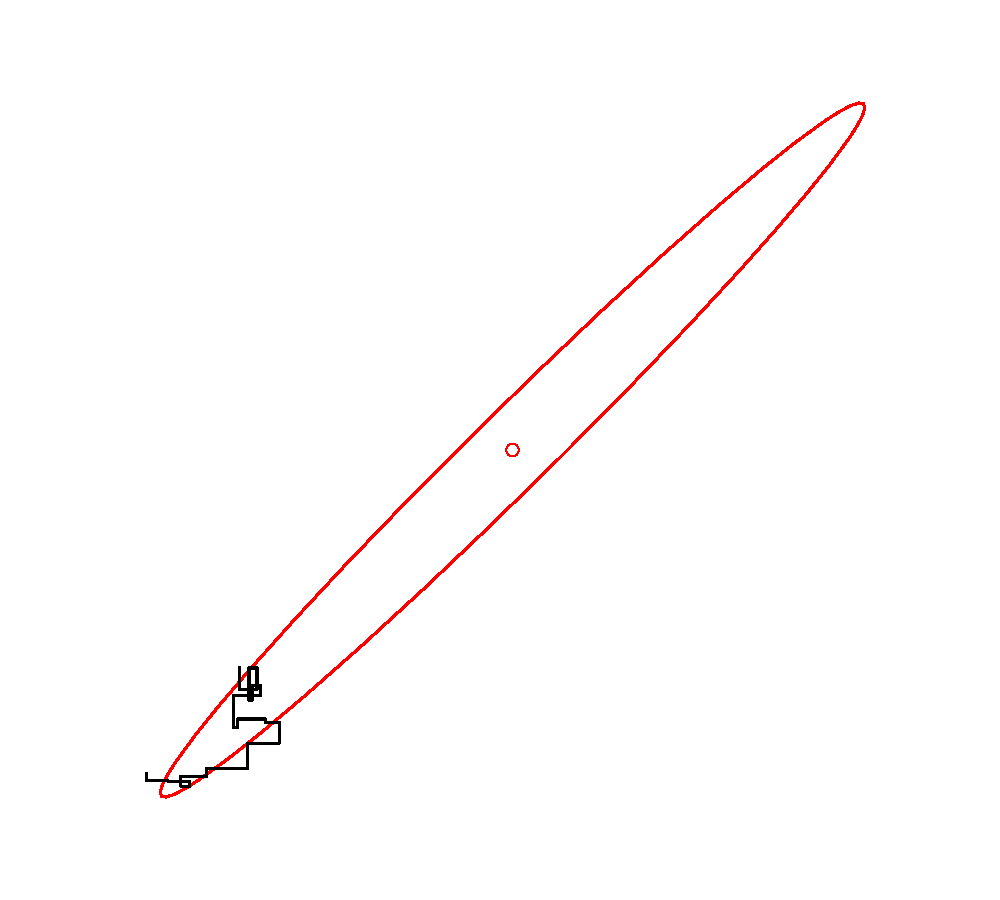
\includegraphics{poormixing.pdf}
\caption{An example of a poorly-mixing sample in two dimensions. Notice that the
chain is trapped in a region of low probability relative to the mean
(dot) and variance (oval) of the true posterior quantity.}\label{modelchecking:mix}\end{figure}


\subsection{Informal Methods}
\label{modelchecking:informal-methods}
The most straightforward approach for assessing convergence is based on simply plotting and inspecting traces and histograms of the observed MCMC sample. If the trace of values for each of the stochastics exhibits asymptotic behavior \footnote{
Asymptotic behaviour implies that the variance and the mean value of the sample
stays relatively constant over some arbitrary period.
} over the last $m$ iterations, this may be satisfactory evidence for convergence. A similar approach involves plotting a histogram for every set of $k$ iterations (perhaps 50-100) beyond some burn in threshold $n$; if the histograms are not visibly different among the sample intervals, this is reasonable evidence for convergence. Note that such diagnostics should be carried out for each stochastic estimated by the MCMC algorithm, because convergent behavior by one variable does not imply evidence for convergence for other variables in the analysis. An extension of this approach can be taken when multiple parallel chains are run, rather than just a single, long chain. In this case, the final values of $c$ chains run for $n$ iterations are plotted in a histogram; just as above, this is repeated every $k$ iterations thereafter, and the histograms of the endpoints are plotted again and compared to the previous histogram. This is repeated until consecutive histograms are indistinguishable.

Another \emph{ad hoc} method for detecting lack of convergence is to examine the traces of several MCMC chains initialized with different starting values. Overlaying these traces on the same set of axes should (if convergence has occurred) show each chain tending toward the same equilibrium value, with approximately the same variance. Recall that the tendency for some Markov chains to converge to the true (unknown) value from diverse initial values is called \emph{ergodicity}. This property is guaranteed by the reversible chains constructed using MCMC, and should be observable using this technique. Again, however, this approach is only a heuristic method, and cannot always detect lack of convergence, even though chains may appear ergodic.
\begin{figure}[htbp]
\centering
\capstart

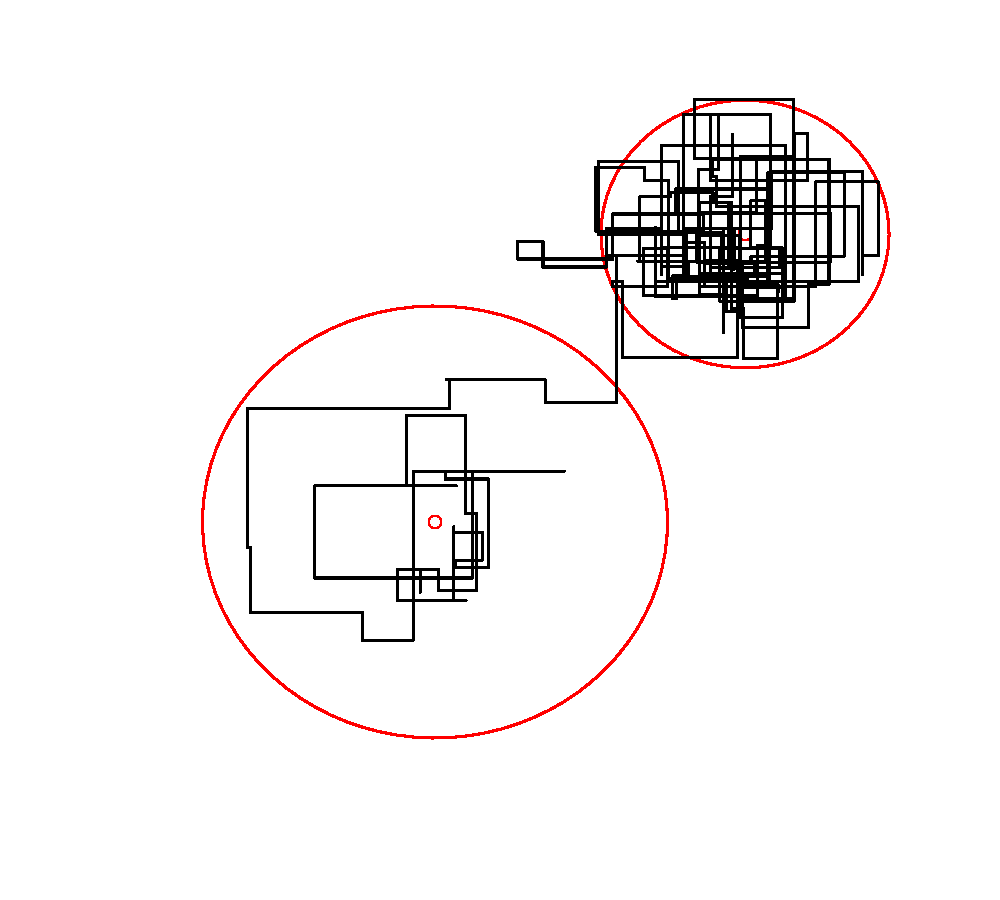
\includegraphics{metastable.pdf}
\caption{An example of metastability in a two-dimensional parameter space. The
chain appears to be stable in one region of the parameter space for an
extended period, then unpredictably jumps to another region of the
space.}\label{modelchecking:metas}\end{figure}

A principal reason that evidence from informal techniques cannot guarantee convergence is a phenomenon called metastability. Chains may appear to have converged to the true equilibrium value, displaying excellent qualities by any of the methods described above. However, after some period of stability around this value, the chain may suddenly move to another region of the parameter space (Figure {\hyperref[modelchecking:metas]{\emph{An example of metastability in a two-dimensional parameter space. The
chain appears to be stable in one region of the parameter space for an
extended period, then unpredictably jumps to another region of the
space.}}}). This period of metastability can sometimes be very long, and therefore escape detection by these convergence diagnostics. Unfortunately, there is no statistical technique available for detecting metastability.


\subsection{Formal Methods}
\label{modelchecking:formal-methods}
Along with the \emph{ad hoc} techniques described above, a number of more formal methods exist which are prevalent in the literature. These are considered more formal because they are based on existing statistical methods, such as time series analysis.

PyMC currently includes two formal convergence diagnostic methods. The first, proposed by {\hyperref[references:geweke-1992]{{[}Geweke\_1992{]}}}, is a time-series approach that compares the mean and variance of segments from the beginning and end of a single chain.
\begin{gather}
\begin{split}z = \frac{\bar{\theta}_a - \bar{\theta}_b}{\sqrt{Var(\theta_a) + Var(\theta_b)}}\end{split}\notag\\\begin{split}\end{split}\notag
\end{gather}
where $a$ is the early interval and $b$ the late interval. If the z-scores (theoretically distributed as standard normal variates) of these two segments are similar, it can provide evidence for convergence. PyMC calculates z-scores of the difference between various initial segments along the chain, and the last 50\% of the remaining chain. If the chain has converged, the majority of points should fall within 2 standard deviations of zero.

Diagnostic z-scores can be obtained by calling the \code{geweke} function. It accepts either (1) a single trace, (2) a Node or Stochastic object, or (4) an entire Model object:

\begin{Verbatim}[commandchars=\\\{\}]
\PYG{n}{geweke}\PYG{p}{(}\PYG{n}{x}\PYG{p}{,} \PYG{n}{first}\PYG{o}{=}\PYG{l+m+mf}{0.1}\PYG{p}{,} \PYG{n}{last}\PYG{o}{=}\PYG{l+m+mf}{0.5}\PYG{p}{,} \PYG{n}{intervals}\PYG{o}{=}\PYG{l+m+mi}{20}\PYG{p}{)}
\end{Verbatim}

The arguments expected are the following:
\begin{itemize}
\item {} 
\code{pymc\_object}: The object that is or contains the output trace(s).

\item {} 
\code{first} (optional): First portion of chain to be used in Geweke diagnostic. Defaults to 0.1 (\emph{i.e.} first 10\% of chain).

\item {} 
\code{last} (optional): Last portion of chain to be used in Geweke diagnostic. Defaults to 0.5 (\emph{i.e.} last 50\% of chain).

\item {} 
\code{intervals} (optional): Number of sub-chains to analyze. Defaults to 20.

\end{itemize}

The resulting scores are best interpreted graphically, using the \code{geweke\_plot} function. This displays the scores in series, in relation to the 2 standard deviation boundaries around zero. Hence, it is easy to see departures from the standard normal assumption.
\begin{figure}[htbp]
\centering
\capstart

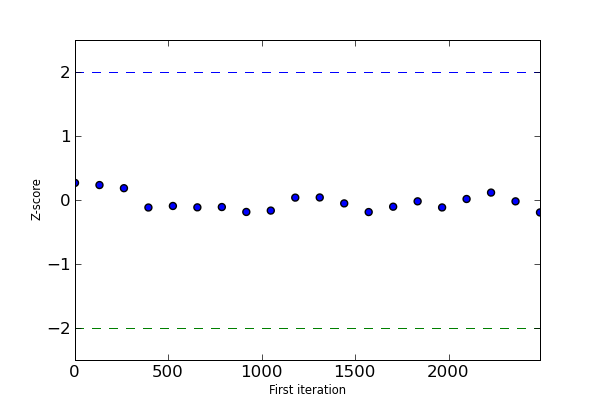
\includegraphics{geweke.png}
\caption{Sample plot of Geweke z-scores for a variable using \code{geweke\_plot}.
The occurrence of the scores well within 2 standard deviations of zero
gives not indicate of lack of convergence (top), while deviations exceeding
2 standard deviations suggest that additional samples are requred to
achieve convergence (bottom).}\label{modelchecking:geweke}\end{figure}

\code{geweke\_plot} takes either a single set of scores, or a dictionary of scores (output by \code{geweke} when an entire Sampler is passed) as its argument:

\begin{Verbatim}[commandchars=@\[\]]
def geweke@_plot(scores, name='geweke', format='png', suffix='-diagnostic',
                path='./', fontmap = {1:10, 2:8, 3:6, 4:5, 5:4}, verbose=1)
\end{Verbatim}

The arguments are defined as:
\begin{itemize}
\item {} 
\code{scores}: The object that contains the Geweke scores. Can be a list (one set) or a dictionary (multiple sets).

\item {} 
\code{name} (optional): Name used for output files. For multiple scores, the dictionary keys are used as names.

\item {} 
\code{format} (optional): Graphic output file format (defaults to \emph{png}).

\item {} 
\code{suffix} (optional): Suffix to filename (defaults to \emph{-diagnostic})

\item {} 
\code{path} (optional): The path for output graphics (defaults to working directory).

\item {} 
\code{fontmap} (optional): Dictionary containing the font map for the labels of the graphic.

\item {} 
\code{verbose} (optional): Verbosity level for output (defaults to 1).

\end{itemize}

To illustrate, consider a model \code{my\_model} that is used to instantiate a MCMC sampler. The sampler is then run for a given number of iterations:

\begin{Verbatim}[commandchars=\\\{\}]
\PYG{g+gp}{\textgreater{}\textgreater{}\textgreater{} }\PYG{n}{S} \PYG{o}{=} \PYG{n}{pymc}\PYG{o}{.}\PYG{n}{MCMC}\PYG{p}{(}\PYG{n}{my\PYGZus{}model}\PYG{p}{)}
\PYG{g+gp}{\textgreater{}\textgreater{}\textgreater{} }\PYG{n}{S}\PYG{o}{.}\PYG{n}{sample}\PYG{p}{(}\PYG{l+m+mi}{10000}\PYG{p}{,} \PYG{n}{burn}\PYG{o}{=}\PYG{l+m+mi}{5000}\PYG{p}{)}
\end{Verbatim}

It is easiest simply to pass the entire sampler \code{S} the \code{geweke} function:

\begin{Verbatim}[commandchars=\\\{\}]
\PYG{g+gp}{\textgreater{}\textgreater{}\textgreater{} }\PYG{n}{scores} \PYG{o}{=} \PYG{n}{pymc}\PYG{o}{.}\PYG{n}{geweke}\PYG{p}{(}\PYG{n}{S}\PYG{p}{,} \PYG{n}{intervals}\PYG{o}{=}\PYG{l+m+mi}{20}\PYG{p}{)}
\PYG{g+gp}{\textgreater{}\textgreater{}\textgreater{} }\PYG{n}{pymc}\PYG{o}{.}\PYG{n}{Matplot}\PYG{o}{.}\PYG{n}{geweke\PYGZus{}plot}\PYG{p}{(}\PYG{n}{scores}\PYG{p}{)}
\end{Verbatim}

Alternatively, individual stochastics within \code{S} can be analyzed for convergence:

\begin{Verbatim}[commandchars=\\\{\}]
\PYG{g+gp}{\textgreater{}\textgreater{}\textgreater{} }\PYG{n}{trace} \PYG{o}{=} \PYG{n}{S}\PYG{o}{.}\PYG{n}{alpha}\PYG{o}{.}\PYG{n}{trace}\PYG{p}{(}\PYG{p}{)}
\PYG{g+gp}{\textgreater{}\textgreater{}\textgreater{} }\PYG{n}{alpha\PYGZus{}scores} \PYG{o}{=} \PYG{n}{pymc}\PYG{o}{.}\PYG{n}{geweke}\PYG{p}{(}\PYG{n}{trace}\PYG{p}{,} \PYG{n}{intervals}\PYG{o}{=}\PYG{l+m+mi}{20}\PYG{p}{)}
\PYG{g+gp}{\textgreater{}\textgreater{}\textgreater{} }\PYG{n}{pymc}\PYG{o}{.}\PYG{n}{Matplot}\PYG{o}{.}\PYG{n}{geweke\PYGZus{}plot}\PYG{p}{(}\PYG{n}{alpha\PYGZus{}scores}\PYG{p}{,} \PYG{l+s}{'}\PYG{l+s}{alpha}\PYG{l+s}{'}\PYG{p}{)}
\end{Verbatim}

An example of convergence and non-convergence of a chain using \emph{geweke\_plot} is given in Figure {\hyperref[modelchecking:geweke]{\emph{Sample plot of Geweke z-scores for a variable using geweke\_plot.
The occurrence of the scores well within 2 standard deviations of zero
gives not indicate of lack of convergence (top), while deviations exceeding
2 standard deviations suggest that additional samples are requred to
achieve convergence (bottom).}}} .

The second diagnostic provided by PyMC is the {\hyperref[references:raftery-1995a]{{[}Raftery\_1995a{]}}} procedure. This approach estimates the number of iterations required to reach convergence, along with the number of burn-in samples to be discarded and the appropriate thinning interval. A separate estimate of both quantities can be obtained for each variable in a given model.

As the criterion for determining convergence, the Raftery and Lewis approach uses the accuracy of estimation of a user-specified quantile. For example, we may want to estimate the quantile $q=0.975$ to within $r=0.005$ with probability $s=0.95$. In other words,
\begin{gather}
\begin{split}Pr(|\hat{q}-q| \le r) = s\end{split}\notag\\\begin{split}\end{split}\notag
\end{gather}
From any sample of $\theta$, one can construct a binary chain:
\begin{gather}
\begin{split}Z^{(j)} = I(\theta^{(j)} \le u_q)\end{split}\notag\\\begin{split}\end{split}\notag
\end{gather}
where $u_q$ is the quantile value and $I$ is the indicator function. While $\{\theta^{(j)}\}$ is a Markov chain, $\{Z^{(j)}\}$ is not necessarily so. In any case, the serial dependency among $Z^{(j)}$ decreases as the thinning interval $k$ increases. A value of $k$ is chosen to be the smallest value such that the first order Markov chain is preferable to the second order Markov chain.

This thinned sample is used to determine number of burn-in samples. This is done by comparing the remaining samples from burn-in intervals of increasing length to the limiting distribution of the chain. An appropriate value is one for which the truncated sample's distribution is within $\epsilon$ (arbitrarily small) of the limiting distribution. See {\hyperref[references:raftery-1995a]{{[}Raftery\_1995a{]}}} or {\hyperref[references:gamerman-1997]{{[}Gamerman\_1997{]}}} for computational details. Estimates for sample size tend to be conservative.

This diagnostic is best used on a short pilot run of a particular model, and the results used to parameterize a subsequent sample that is to be used for inference. Its calling convention is as follows:

\begin{Verbatim}[commandchars=\\\{\}]
\PYG{n}{raftery\PYGZus{}lewis}\PYG{p}{(}\PYG{n}{x}\PYG{p}{,} \PYG{n}{q}\PYG{p}{,} \PYG{n}{r}\PYG{p}{,} \PYG{n}{s}\PYG{o}{=}\PYG{o}{.}\PYG{l+m+mi}{95}\PYG{p}{,} \PYG{n}{epsilon}\PYG{o}{=}\PYG{o}{.}\PYG{l+m+mo}{001}\PYG{p}{,} \PYG{n}{verbose}\PYG{o}{=}\PYG{l+m+mi}{1}\PYG{p}{)}
\end{Verbatim}

The arguments are:
\begin{itemize}
\item {} 
\code{pymc\_object}: The object that contains the Geweke scores. Can be a list (one set) or a dictionary (multiple sets).

\item {} 
\code{q}: Desired quantile to be estimated.

\item {} 
\code{r}: Desired accuracy for quantile.

\item {} 
\code{s} (optional): Probability of attaining the requested accuracy (defaults
to 0.95).

\item {} 
\code{epsilon} (optional) : Half width of the tolerance interval required for the q-quantile (defaults to 0.001).

\item {} 
\code{verbose} (optional) : Verbosity level for output (defaults to 1).

\end{itemize}

The code for \code{raftery\_lewis} is based on the FORTRAN program \emph{gibbsit} ({\hyperref[references:raftery-1995b]{{[}Raftery\_1995b{]}}}).

For example, consider again a sampler S run for some model my\_model:

\begin{Verbatim}[commandchars=\\\{\}]
\PYG{g+gp}{\textgreater{}\textgreater{}\textgreater{} }\PYG{n}{S} \PYG{o}{=} \PYG{n}{pymc}\PYG{o}{.}\PYG{n}{MCMC}\PYG{p}{(}\PYG{n}{my\PYGZus{}model}\PYG{p}{)}
\PYG{g+gp}{\textgreater{}\textgreater{}\textgreater{} }\PYG{n}{S}\PYG{o}{.}\PYG{n}{sample}\PYG{p}{(}\PYG{l+m+mi}{10000}\PYG{p}{,} \PYG{n}{burn}\PYG{o}{=}\PYG{l+m+mi}{5000}\PYG{p}{)}
\end{Verbatim}

One can pass either the entire sampler S or any stochastic within S to the \emph{raftery\_lewis} function, along with suitable arguments. Here, we have chosen $q = 0.025$ (the lower limit of the equal-tailed 95\% interval) and error $r = 0.01$:

\begin{Verbatim}[commandchars=\\\{\}]
\PYG{g+gp}{\textgreater{}\textgreater{}\textgreater{} }\PYG{n}{pymc}\PYG{o}{.}\PYG{n}{raftery\PYGZus{}lewis}\PYG{p}{(}\PYG{n}{S}\PYG{p}{,} \PYG{n}{q}\PYG{o}{=}\PYG{l+m+mf}{0.025}\PYG{p}{,} \PYG{n}{r}\PYG{o}{=}\PYG{l+m+mf}{0.01}\PYG{p}{)}
\end{Verbatim}

This yields diagnostics as follows for each stochastic of S, as well as a dictionary containing the diagnostic quantities:

\begin{Verbatim}[commandchars=@\[\]]
========================
Raftery-Lewis Diagnostic
========================

937 iterations required (assuming independence) to achieve 0.01 accuracy
with 95 percent probability.

Thinning factor of 1 required to produce a first-order Markov chain.

39 iterations to be discarded at the beginning of the simulation (burn-in).

11380 subsequent iterations required.

Thinning factor of 11 required to produce an independence chain.
\end{Verbatim}

Additional convergence diagnostics are available in the \href{http://lib.stat.cmu.edu/r/cran/}{R} statistical
package ({\hyperref[references:r-2010]{{[}R\_2010{]}}}), via the \href{http://www-fis.iarc.fr/coda/}{CODA} module ({\hyperref[references:plummer-2008]{{[}Plummer\_2008{]}}}). PyMC includes a method \code{coda} for exporting model traces in a format that may be directly read by \code{coda}:

\begin{Verbatim}[commandchars=\\\{\}]
\PYG{n}{pymc}\PYG{o}{.}\PYG{n}{utils}\PYG{o}{.}\PYG{n}{coda}\PYG{p}{(}\PYG{n}{pymc\PYGZus{}object}\PYG{p}{)}
\end{Verbatim}

The lone argument is the PyMC sampler for which output is desired.

Calling \code{coda} yields a file containing raw trace values (suffix \code{.out}) and a file containing indices to the trace values (suffix \code{.ind}).


\section{Autocorrelation Plots}
\label{modelchecking:autocorrelation-plots}
Samples from MCMC algorithms are ususally autocorrelated, due partly to the inherent Markovian dependence structure. The degree of autocorrelation can be quantified using the autocorrelation function:
\begin{gather}
\begin{split}\rho_k & = \frac{\mbox{Cov}(X_t,  X_{t+k})}{\sqrt{\mbox{Var}(X_t)\mbox{Var}(X_{t+k})}}\end{split}\notag\\\begin{split}      & = \frac{E[(X_t - \theta)(X_{t+k} - \theta)]}{\sqrt{E[(X_t - \theta)^2] E[(X_{t+k} - \theta)^2]}}\end{split}\notag
\end{gather}
PyMC includes a function for plotting the autocorrelation function for each stochastics in the sampler (Figure {\hyperref[modelchecking:autocorr]{\emph{Sample autocorrelation plots for two Poisson variables from coal mining
disasters example model.}}}). This allows users to examine the relationship among successive samples within sampled chains. Significant autocorrelation suggests that chains require thinning prior to use of the posterior statistics for inference.

\begin{Verbatim}[commandchars=\\\{\}]
\PYG{n}{autocorrelation}\PYG{p}{(}\PYG{n}{pymc\PYGZus{}object}\PYG{p}{,} \PYG{n}{name}\PYG{p}{,} \PYG{n}{maxlag}\PYG{o}{=}\PYG{l+m+mi}{100}\PYG{p}{,} \PYG{n}{format}\PYG{o}{=}\PYG{l+s}{'}\PYG{l+s}{png}\PYG{l+s}{'}\PYG{p}{,} \PYG{n}{suffix}\PYG{o}{=}\PYG{l+s}{'}\PYG{l+s}{-acf}\PYG{l+s}{'}\PYG{p}{,}
\PYG{n}{path}\PYG{o}{=}\PYG{l+s}{'}\PYG{l+s}{./}\PYG{l+s}{'}\PYG{p}{,} \PYG{n}{fontmap} \PYG{o}{=} \PYG{p}{\PYGZob{}}\PYG{l+m+mi}{1}\PYG{p}{:}\PYG{l+m+mi}{10}\PYG{p}{,} \PYG{l+m+mi}{2}\PYG{p}{:}\PYG{l+m+mi}{8}\PYG{p}{,} \PYG{l+m+mi}{3}\PYG{p}{:}\PYG{l+m+mi}{6}\PYG{p}{,} \PYG{l+m+mi}{4}\PYG{p}{:}\PYG{l+m+mi}{5}\PYG{p}{,} \PYG{l+m+mi}{5}\PYG{p}{:}\PYG{l+m+mi}{4}\PYG{p}{\PYGZcb{}}\PYG{p}{,} \PYG{n}{verbose}\PYG{o}{=}\PYG{l+m+mi}{1}\PYG{p}{)}
\end{Verbatim}
\begin{itemize}
\item {} 
\code{pymc\_object}: The object that is or contains the output trace(s).

\item {} 
\code{name}: Name used for output files.

\item {} 
\code{maxlag}: The highest lag interval for which autocorrelation is calculated.

\item {} 
\code{format} (optional): Graphic output file format (defaults to \emph{png}).

\item {} 
\code{suffix} (optional): Suffix to filename (defaults to \emph{-diagnostic})

\item {} 
\code{path} (optional): The path for output graphics (defaults to working directory).

\item {} 
\code{fontmap} (optional): Dictionary containing the font map for the labels of the graphic.

\item {} 
\code{verbose} (optional): Verbosity level for output (defaults to 1).

\end{itemize}

Using any given model \emph{my\_model} as an example, autocorrelation plots can be obtained simply by passing the sampler for that model to the \emph{autocorrelation} function (within the \emph{Matplot} module) directly:

\begin{Verbatim}[commandchars=\\\{\}]
\PYG{g+gp}{\textgreater{}\textgreater{}\textgreater{} }\PYG{n}{S} \PYG{o}{=} \PYG{n}{pymc}\PYG{o}{.}\PYG{n}{MCMC}\PYG{p}{(}\PYG{n}{my\PYGZus{}model}\PYG{p}{)}
\PYG{g+gp}{\textgreater{}\textgreater{}\textgreater{} }\PYG{n}{S}\PYG{o}{.}\PYG{n}{sample}\PYG{p}{(}\PYG{l+m+mi}{10000}\PYG{p}{,} \PYG{n}{burn}\PYG{o}{=}\PYG{l+m+mi}{5000}\PYG{p}{)}
\PYG{g+gp}{\textgreater{}\textgreater{}\textgreater{} }\PYG{n}{pymc}\PYG{o}{.}\PYG{n}{Matplot}\PYG{o}{.}\PYG{n}{autocorrelation}\PYG{p}{(}\PYG{n}{S}\PYG{p}{)}
\end{Verbatim}

Alternatively, variables within a model can be plotted individually. For example, a hypothetical variable \emph{beta} that was estimated using sampler \emph{S} will yield a correlation plot as follows:

\begin{Verbatim}[commandchars=\\\{\}]
\PYG{g+gp}{\textgreater{}\textgreater{}\textgreater{} }\PYG{n}{pymc}\PYG{o}{.}\PYG{n}{Matplot}\PYG{o}{.}\PYG{n}{autocorrelation}\PYG{p}{(}\PYG{n}{S}\PYG{o}{.}\PYG{n}{beta}\PYG{p}{)}
\end{Verbatim}
\begin{figure}[htbp]
\centering
\capstart

\scalebox{0.700000}{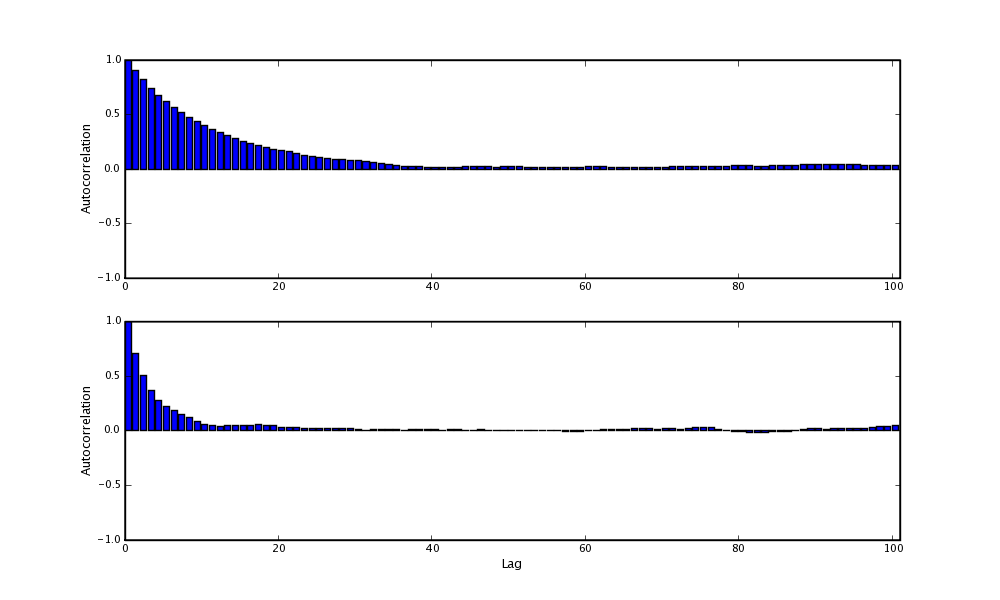
\includegraphics{autocorr.png}}
\caption{Sample autocorrelation plots for two Poisson variables from coal mining
disasters example model.}\label{modelchecking:autocorr}\end{figure}


\section{Goodness of Fit}
\label{modelchecking:goodness-of-fit}
Checking for model convergence is only the first step in the evaluation of MCMC model outputs. It is possible for an entirely unsuitable model to converge, so additional steps are needed to ensure that the estimated model adequately fits the data. One intuitive way for evaluating model fit is to compare model predictions with actual observations. In other words, the fitted model can be used to simulate data, and the distribution of the simulated data should resemble the distribution of the actual data.

Fortunately, simulating data from the model is a natural component of the Bayesian modelling framework. Recall, from the discussion on imputation of missing data, the posterior predictive distribution:
\begin{gather}
\begin{split}p(\tilde{y}|y) = \int p(\tilde{y}|\theta) f(\theta|y) d\theta\end{split}\notag\\\begin{split}\end{split}\notag
\end{gather}
Here, $\tilde{y}$ represents some hypothetical new data that would be expected, taking into account the posterior uncertainty in the model parameters. Sampling from the posterior predictive distribution is easy in PyMC. The code looks identical to the corresponding data stochastic, with two modifications: (1) the node should be specified as deterministic and (2) the statistical likelihoods should be replaced by random number generators. As an example, consider a simple dose-response model, where deaths are modeled as a binomial random variable for which the probability of death is a logit-linear function of the dose of a particular drug:

\begin{Verbatim}[commandchars=@\[\]]
n = @PYGZlb[]5@PYGZrb[]*4
     dose = @PYGZlb[]-.86,-.3,-.05,.73@PYGZrb[]
     x = @PYGZlb[]0,1,3,5@PYGZrb[]

     alpha = pymc.Normal('alpha', mu=0.0, tau=0.01)
     beta = pymc.Normal('beta', mu=0.0, tau=0.01)

     @PYGZat[]pymc.deterministic
     def theta(a=alpha, b=beta, d=dose):
             """theta = inv@_logit(a+b)"""
             return pymc.invlogit(a+b*d)

     """deaths @textasciitilde[] binomial(n, p)"""
     deaths = pymc.Binomial('deaths', n=n, p=theta, value=x, observed=True)
\end{Verbatim}

The posterior predictive distribution of deaths uses the same functional form as the data likelihood, in this case a binomial stochastic. Here is the corresponding sample from the posterior predictive distribution:

\begin{Verbatim}[commandchars=\\\{\}]
\PYG{n+nd}{@pymc.deterministic}
\PYG{k}{def} \PYG{n+nf}{deaths\PYGZus{}sim}\PYG{p}{(}\PYG{n}{n}\PYG{o}{=}\PYG{n}{n}\PYG{p}{,} \PYG{n}{p}\PYG{o}{=}\PYG{n}{theta}\PYG{p}{)}\PYG{p}{:}
        \PYG{l+s+sd}{"""deaths\PYGZus{}sim = rbinomial(n, p)"""}
        \PYG{k}{return} \PYG{n}{pymc}\PYG{o}{.}\PYG{n}{rbinomial}\PYG{p}{(}\PYG{n}{n}\PYG{p}{,} \PYG{n}{p}\PYG{p}{)}
\end{Verbatim}

Notice that the stochastic \emph{pymc.Binomial} has been replaced with a deterministic node that simulates values using \emph{pymc.rbinomial} and the unknown parameters \emph{theta}.

The degree to which simulated data correspond to observations can be evaluated in at least two ways. First, these quantities can simply be compared visually. This allows for a qualitative comparison of model-based replicates and observations. If there is poor fit, the true value of the data may appear in the tails of the histogram of replicated data, while a good fit will tend to show the true data in high-probability regions of the posterior predictive distribution (Figure {\hyperref[modelchecking:gof]{\emph{Data sampled from the posterior predictive distribution of a model for
some observation . The true value of
 is shown by the dotted red line.}}}).
\begin{figure}[htbp]
\centering
\capstart

\scalebox{0.700000}{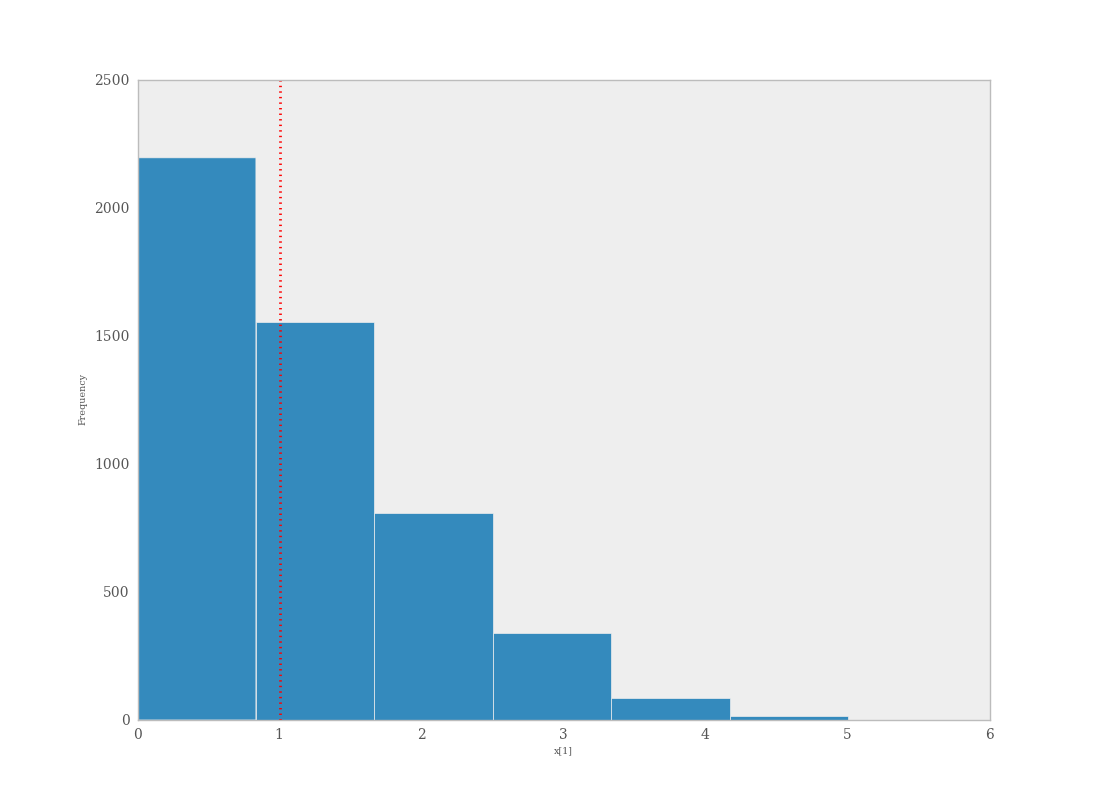
\includegraphics{gof.png}}
\caption{Data sampled from the posterior predictive distribution of a model for
some observation $\mathbf{x}$. The true value of
$\mathbf{x}$ is shown by the dotted red line.}\label{modelchecking:gof}\end{figure}

The Matplot package in PyMC provides an easy way of producing such plots, via the \code{gof\_plot} function. To illustrate, consider a single data point \code{x} and an array of values \code{x\_sim} sampled from the posterior predictive distribution. The histogram is generated by calling:

\begin{Verbatim}[commandchars=\\\{\}]
\PYG{n}{pymc}\PYG{o}{.}\PYG{n}{Matplot}\PYG{o}{.}\PYG{n}{gof\PYGZus{}plot}\PYG{p}{(}\PYG{n}{x\PYGZus{}sim}\PYG{p}{,} \PYG{n}{x}\PYG{p}{,} \PYG{n}{name}\PYG{o}{=}\PYG{l+s}{'}\PYG{l+s}{x}\PYG{l+s}{'}\PYG{p}{)}
\end{Verbatim}

A second approach for evaluating goodness of fit using samples from the posterior predictive distribution involves the use of a statistical criterion. For example, the Bayesian p-value {\hyperref[references:gelman-1996]{{[}Gelman\_1996{]}}} uses a discrepancy measure that quantifies the difference between data (observed or simulated) and the expected value, conditional on some model. One such discrepancy measure is the Freeman-Tukey statistic {\hyperref[references:brooks-2000]{{[}Brooks\_2000{]}}}:
\begin{gather}
\begin{split}D(x|\theta) = \sum_j (\sqrt{x_j}-\sqrt{e_j})^2\end{split}\notag
\end{gather}
Model fit is assessed by comparing the discrepancies from observed data to those from simulated data. On average, we expect the difference between them to be zero; hence, the Bayesian \emph{p} value is simply the proportion of simulated discrepancies that are larger than their corresponding observed discrepancies:
\begin{gather}
\begin{split}p = Pr[ D(\text{sim}) > D(\text{obs}) ]\end{split}\notag\\\begin{split}\end{split}\notag
\end{gather}
If $p$ is very large (e.g. $>0.975$) or very small (e.g. $<0.025$) this implies that the model is not consistent with the data, and thus is evidence of lack of fit. Graphically, data and simulated discrepancies plotted together should be clustered along a 45 degree line passing through the origin, as shown in Figure {\hyperref[modelchecking:deviate]{\emph{Plot of deviates of observed and simulated data from expected values.
The cluster of points symmetrically about the 45 degree line (and the
reported p-value) suggests acceptable fit for the modeled parameter.}}}.
\begin{figure}[htbp]
\centering
\capstart

\scalebox{1.000000}{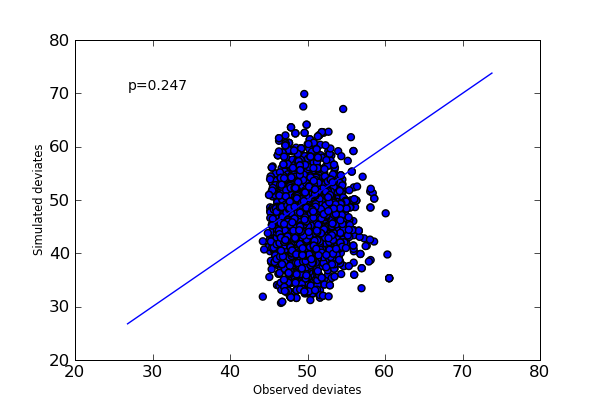
\includegraphics{deviates.png}}
\caption{Plot of deviates of observed and simulated data from expected values.
The cluster of points symmetrically about the 45 degree line (and the
reported p-value) suggests acceptable fit for the modeled parameter.}\label{modelchecking:deviate}\end{figure}

The \code{discrepancy} function in the \code{diagnostics} package can be used to generate discrepancy statistics from arrays of data, simulated values, and expected values:

\begin{Verbatim}[commandchars=\\\{\}]
\PYG{n}{D} \PYG{o}{=} \PYG{n}{pymc}\PYG{o}{.}\PYG{n}{utils}\PYG{o}{.}\PYG{n}{discrepancy}\PYG{p}{(}\PYG{n}{x}\PYG{p}{,} \PYG{n}{x\PYGZus{}sim}\PYG{p}{,} \PYG{n}{x\PYGZus{}exp}\PYG{p}{)}
\end{Verbatim}

A call to this function returns two arrays of discrepancy values, which can be passed to the \code{discrepancy\_plot} function in the \emph{Matplot} module to generate a scatter plot, and if desired, a \emph{p} value:

\begin{Verbatim}[commandchars=\\\{\}]
\PYG{n}{pymc}\PYG{o}{.}\PYG{n}{Matplot}\PYG{o}{.}\PYG{n}{discrepancy\PYGZus{}plot}\PYG{p}{(}\PYG{n}{D}\PYG{p}{,} \PYG{n}{name}\PYG{o}{=}\PYG{l+s}{'}\PYG{l+s}{D}\PYG{l+s}{'}\PYG{p}{,} \PYG{n}{report\PYGZus{}p}\PYG{o}{=}\PYG{n+nb+bp}{True}\PYG{p}{)}
\end{Verbatim}

Additional optional arguments for \code{discrepancy\_plot} are identical to other PyMC plotting functions.


\chapter{Extending PyMC}
\label{extending:chap-extending}\label{extending::doc}\label{extending:extending-pymc}
PyMC tries to make standard things easy, but keep unusual things possible. Its openness, combined with Python's flexibility, invite extensions from using new step methods to exotic stochastic processes (see the Gaussian process module). This chapter briefly reviews the ways PyMC is designed to be extended.


\section{Nonstandard Stochastics}
\label{extending:nonstandard-stochastics}\label{extending:nonstandard}
The simplest way to create a \code{Stochastic} object with a nonstandard distribution is to use the medium or long decorator syntax. See Chapter {\hyperref[modelbuilding:chap-modelbuilding]{\emph{Building models}}}. If you want to create many stochastics with the same nonstandard distribution, the decorator syntax can become cumbersome. An actual subclass of \code{Stochastic} can be created using the class factory \code{stochastic\_from\_dist}. This function takes the following arguments:
\begin{itemize}
\item {} 
The name of the new class,

\item {} 
A \code{logp} function,

\item {} 
A \code{random} function,

\item {} 
The NumPy datatype of the new class (for continuous distributions, this should be \code{float}; for discrete distributions, \code{int}; for variables valued as non-numerical objects, \code{object}),

\item {} 
A flag indicating whether the resulting class represents a vector-valued variable.

\end{itemize}

The necessary parent labels are read from the \code{logp} function, and a docstring for the new class is automatically generated. Instances of the new class can be created in one line.

Full subclasses of \code{Stochastic} may be necessary to provide nonstandard behaviors (see \code{gp.GP}).


\section{User-defined step methods}
\label{extending:custom-stepper}\label{extending:user-defined-step-methods}
The \code{StepMethod} class is meant to be subclassed. There are an enormous number of MCMC step methods in the literature, whereas PyMC provides only about half a dozen. Most user-defined step methods will be either Metropolis-Hastings or Gibbs step methods, and these should subclass \code{Metropolis} or \code{Gibbs} respectively. More unusual step methods should subclass \code{StepMethod} directly.


\subsection{Example: an asymmetric Metropolis step}
\label{extending:example-an-asymmetric-metropolis-step}
Consider the probability model in \code{examples/custom\_step.py}:

\begin{Verbatim}[commandchars=\\\{\}]
\PYG{n}{mu} \PYG{o}{=} \PYG{n}{pymc}\PYG{o}{.}\PYG{n}{Normal}\PYG{p}{(}\PYG{l+s}{'}\PYG{l+s}{mu}\PYG{l+s}{'}\PYG{p}{,}\PYG{l+m+mi}{0}\PYG{p}{,}\PYG{o}{.}\PYG{l+m+mo}{01}\PYG{p}{,} \PYG{n}{value}\PYG{o}{=}\PYG{l+m+mi}{0}\PYG{p}{)}
\PYG{n}{tau} \PYG{o}{=} \PYG{n}{pymc}\PYG{o}{.}\PYG{n}{Exponential}\PYG{p}{(}\PYG{l+s}{'}\PYG{l+s}{tau}\PYG{l+s}{'}\PYG{p}{,}\PYG{o}{.}\PYG{l+m+mo}{01}\PYG{p}{,} \PYG{n}{value}\PYG{o}{=}\PYG{l+m+mi}{1}\PYG{p}{)}
\PYG{n}{cutoff} \PYG{o}{=} \PYG{n}{pymc}\PYG{o}{.}\PYG{n}{Exponential}\PYG{p}{(}\PYG{l+s}{'}\PYG{l+s}{cutoff}\PYG{l+s}{'}\PYG{p}{,}\PYG{l+m+mi}{1}\PYG{p}{,} \PYG{n}{value}\PYG{o}{=}\PYG{l+m+mf}{1.3}\PYG{p}{)}
\PYG{n}{D} \PYG{o}{=} \PYG{n}{pymc}\PYG{o}{.}\PYG{n}{Truncnorm}\PYG{p}{(}\PYG{l+s}{'}\PYG{l+s}{D}\PYG{l+s}{'}\PYG{p}{,}\PYG{n}{mu}\PYG{p}{,}\PYG{n}{tau}\PYG{p}{,}\PYG{o}{-}\PYG{n}{np}\PYG{o}{.}\PYG{n}{inf}\PYG{p}{,}\PYG{n}{cutoff}\PYG{p}{,}\PYG{n}{value}\PYG{o}{=}\PYG{n}{data}\PYG{p}{,}\PYG{n}{observed}\PYG{o}{=}\PYG{n+nb+bp}{True}\PYG{p}{)}
\end{Verbatim}

The stochastic variable \code{cutoff} cannot be smaller than the largest element of $D$, otherwise $D$`s density would be zero. The standard \code{Metropolis} step method can handle this case without problems; it will propose illegal values occasionally, but these will be rejected.

Suppose we want to handle \code{cutoff} with a smarter step method that doesn't propose illegal values. Specifically, we want to use the nonsymmetric proposal distribution
\begin{eqnarray*}
      x_p | x \sim \textup{Truncnorm}(x, \sigma, \max(D), \infty).
\end{eqnarray*}
We can implement this Metropolis-Hastings algorithm with the following step method class:

\begin{Verbatim}[commandchars=\\\{\}]
\PYG{k}{class} \PYG{n+nc}{TruncatedMetropolis}\PYG{p}{(}\PYG{n}{pymc}\PYG{o}{.}\PYG{n}{Metropolis}\PYG{p}{)}\PYG{p}{:}
    \PYG{k}{def} \PYG{n+nf}{\PYGZus{}\PYGZus{}init\PYGZus{}\PYGZus{}}\PYG{p}{(}\PYG{n+nb+bp}{self}\PYG{p}{,} \PYG{n}{stochastic}\PYG{p}{,} \PYG{n}{low\PYGZus{}bound}\PYG{p}{,} \PYG{n}{up\PYGZus{}bound}\PYG{p}{,} \PYG{o}{*}\PYG{n}{args}\PYG{p}{,} \PYG{o}{*}\PYG{o}{*}\PYG{n}{kwargs}\PYG{p}{)}\PYG{p}{:}
        \PYG{n+nb+bp}{self}\PYG{o}{.}\PYG{n}{low\PYGZus{}bound} \PYG{o}{=} \PYG{n}{low\PYGZus{}bound}
        \PYG{n+nb+bp}{self}\PYG{o}{.}\PYG{n}{up\PYGZus{}bound} \PYG{o}{=} \PYG{n}{up\PYGZus{}bound}
        \PYG{n}{pymc}\PYG{o}{.}\PYG{n}{Metropolis}\PYG{o}{.}\PYG{n}{\PYGZus{}\PYGZus{}init\PYGZus{}\PYGZus{}}\PYG{p}{(}\PYG{n+nb+bp}{self}\PYG{p}{,} \PYG{n}{stochastic}\PYG{p}{,} \PYG{o}{*}\PYG{n}{args}\PYG{p}{,} \PYG{o}{*}\PYG{o}{*}\PYG{n}{kwargs}\PYG{p}{)}

    \PYG{k}{def} \PYG{n+nf}{propose}\PYG{p}{(}\PYG{n+nb+bp}{self}\PYG{p}{)}\PYG{p}{:}
        \PYG{n}{tau} \PYG{o}{=} \PYG{l+m+mf}{1.}\PYG{o}{/}\PYG{p}{(}\PYG{n+nb+bp}{self}\PYG{o}{.}\PYG{n}{adaptive\PYGZus{}scale\PYGZus{}factor} \PYG{o}{*} \PYG{n+nb+bp}{self}\PYG{o}{.}\PYG{n}{proposal\PYGZus{}sd}\PYG{p}{)}\PYG{o}{*}\PYG{o}{*}\PYG{l+m+mi}{2}
        \PYG{n+nb+bp}{self}\PYG{o}{.}\PYG{n}{stochastic}\PYG{o}{.}\PYG{n}{value} \PYG{o}{=} \PYGZbs{}
        \PYG{n}{pymc}\PYG{o}{.}\PYG{n}{rtruncnorm}\PYG{p}{(}\PYG{n+nb+bp}{self}\PYG{o}{.}\PYG{n}{stochastic}\PYG{o}{.}\PYG{n}{value}\PYG{p}{,} \PYG{n}{tau}\PYG{p}{,} \PYG{n+nb+bp}{self}\PYG{o}{.}\PYG{n}{low\PYGZus{}bound}\PYG{p}{,} \PYG{n+nb+bp}{self}\PYG{o}{.}\PYG{n}{up\PYGZus{}bound}\PYG{p}{)}

    \PYG{k}{def} \PYG{n+nf}{hastings\PYGZus{}factor}\PYG{p}{(}\PYG{n+nb+bp}{self}\PYG{p}{)}\PYG{p}{:}
        \PYG{n}{tau} \PYG{o}{=} \PYG{l+m+mf}{1.}\PYG{o}{/}\PYG{p}{(}\PYG{n+nb+bp}{self}\PYG{o}{.}\PYG{n}{adaptive\PYGZus{}scale\PYGZus{}factor} \PYG{o}{*} \PYG{n+nb+bp}{self}\PYG{o}{.}\PYG{n}{proposal\PYGZus{}sd}\PYG{p}{)}\PYG{o}{*}\PYG{o}{*}\PYG{l+m+mi}{2}
        \PYG{n}{cur\PYGZus{}val} \PYG{o}{=} \PYG{n+nb+bp}{self}\PYG{o}{.}\PYG{n}{stochastic}\PYG{o}{.}\PYG{n}{value}
        \PYG{n}{last\PYGZus{}val} \PYG{o}{=} \PYG{n+nb+bp}{self}\PYG{o}{.}\PYG{n}{stochastic}\PYG{o}{.}\PYG{n}{last\PYGZus{}value}

        \PYG{n}{lp\PYGZus{}for} \PYG{o}{=} \PYG{n}{pymc}\PYG{o}{.}\PYG{n}{truncnorm\PYGZus{}like}\PYG{p}{(}\PYG{n}{cur\PYGZus{}val}\PYG{p}{,} \PYG{n}{last\PYGZus{}val}\PYG{p}{,} \PYG{n}{tau}\PYG{p}{,} \PYG{n+nb+bp}{self}\PYG{o}{.}\PYG{n}{low\PYGZus{}bound}\PYG{p}{,} \PYG{n+nb+bp}{self}\PYG{o}{.}\PYG{n}{up\PYGZus{}bound}\PYG{p}{)}
        \PYG{n}{lp\PYGZus{}bak} \PYG{o}{=} \PYG{n}{pymc}\PYG{o}{.}\PYG{n}{truncnorm\PYGZus{}like}\PYG{p}{(}\PYG{n}{last\PYGZus{}val}\PYG{p}{,} \PYG{n}{cur\PYGZus{}val}\PYG{p}{,} \PYG{n}{tau}\PYG{p}{,} \PYG{n+nb+bp}{self}\PYG{o}{.}\PYG{n}{low\PYGZus{}bound}\PYG{p}{,} \PYG{n+nb+bp}{self}\PYG{o}{.}\PYG{n}{up\PYGZus{}bound}\PYG{p}{)}

        \PYG{k}{if} \PYG{n+nb+bp}{self}\PYG{o}{.}\PYG{n}{verbose} \PYG{o}{\textgreater{}} \PYG{l+m+mi}{1}\PYG{p}{:}
            \PYG{k}{print} \PYG{n+nb+bp}{self}\PYG{o}{.}\PYG{n}{\PYGZus{}id} \PYG{o}{+} \PYG{l+s}{'}\PYG{l+s}{: Hastings factor }\PYG{l+s+si}{\PYGZpc{}f}\PYG{l+s}{'}\PYG{o}{\PYGZpc{}}\PYG{p}{(}\PYG{n}{lp\PYGZus{}bak} \PYG{o}{-} \PYG{n}{lp\PYGZus{}for}\PYG{p}{)}
        \PYG{k}{return} \PYG{n}{lp\PYGZus{}bak} \PYG{o}{-} \PYG{n}{lp\PYGZus{}for}
\end{Verbatim}

The \code{propose} method sets the step method's stochastic's value to a new value, drawn from a truncated normal distribution. The precision of this distribution is computed from two factors: \code{self.proposal\_sd}, which can be set with an input argument to Metropolis, and \code{self.adaptive\_scale\_factor}. Metropolis step methods' default tuning behavior is to reduce \code{adaptive\_scale\_factor} if the acceptance rate is too low, and to increase \code{adaptive\_scale\_factor} if it is too high. By incorporating \code{adaptive\_scale\_factor} into the proposal standard deviation, we avoid having to write our own tuning infrastructure. If we don't want the proposal to tune, we don't have to use \code{adaptive\_scale\_factor}.

The \code{hastings\_factor} method adjusts for the asymmetric proposal distribution {\hyperref[references:gelman-2004]{{[}Gelman\_2004{]}}}. It computes the log of the quotient of the `backward' density and the `forward' density. For symmetric proposal distributions, this quotient is 1, so its log is zero.

Having created our custom step method, we need to tell MCMC instances to use it to handle the variable \code{cutoff}. This is done in \code{custom\_step.py} with the following line:

\begin{Verbatim}[commandchars=\\\{\}]
\PYG{n}{M}\PYG{o}{.}\PYG{n}{use\PYGZus{}step\PYGZus{}method}\PYG{p}{(}\PYG{n}{TruncatedMetropolis}\PYG{p}{,} \PYG{n}{cutoff}\PYG{p}{,} \PYG{n}{D}\PYG{o}{.}\PYG{n}{value}\PYG{o}{.}\PYG{n}{max}\PYG{p}{(}\PYG{p}{)}\PYG{p}{,} \PYG{n}{np}\PYG{o}{.}\PYG{n}{inf}\PYG{p}{)}
\end{Verbatim}

This call causes $M$ to pass the arguments \code{cutoff}, \code{D.value.max()}, and \code{np.inf} to a \code{TruncatedMetropolis} object's \code{\_\_init\_\_} method, and use the object to handle \code{cutoff}.

Its often convenient to get a handle to a custom step method instance directly for debugging purposes. \code{M.step\_method\_dict{[}cutoff{]}} returns a list of all the step methods $M$ will use to handle \code{cutoff}:

\begin{Verbatim}[commandchars=\\\{\}]
\PYG{g+gp}{\textgreater{}\textgreater{}\textgreater{} }\PYG{n}{M}\PYG{o}{.}\PYG{n}{step\PYGZus{}method\PYGZus{}dict}\PYG{p}{[}\PYG{n}{cutoff}\PYG{p}{]}
\PYG{g+go}{[\textless{}custom\PYGZus{}step.TruncatedMetropolis object at 0x3c91130\textgreater{}]}
\end{Verbatim}

There may be more than one, and conversely step methods may handle more than one stochastic variable. To see which variables step method $S$ is handling, try:

\begin{Verbatim}[commandchars=\\\{\}]
\PYG{g+gp}{\textgreater{}\textgreater{}\textgreater{} }\PYG{n}{S}\PYG{o}{.}\PYG{n}{stochastics}
\PYG{g+go}{set([\textless{}pymc.distributions.Exponential 'cutoff' at 0x3cd6b90\textgreater{}])}
\end{Verbatim}


\subsection{General step methods}
\label{extending:general-step-methods}
All step methods must implement the following methods:
\begin{description}
\item[{\code{step()}:}] \leavevmode
Updates the values of \code{self.stochastics}.

\item[{\code{tune()}:}] \leavevmode
Tunes the jumping strategy based on performance so far. A default method is
available that increases \code{self.adaptive\_scale\_factor} (see below) when
acceptance rate is high, and decreases it when acceptance rate is low. This
method should return \code{True} if additional tuning will be required later,
\begin{quote}

and \code{False} otherwise.
\end{quote}

\item[{\code{competence(s):}}] \leavevmode\begin{description}
\item[{A class method that examines stochastic variable $s$ and returns a}] \leavevmode
value from 0 to 3 expressing the step method's ability to handle the
variable. This method is used by \code{MCMC} instances when automatically
assigning step methods. Conventions are:

\item[{0}] \leavevmode
I cannot safely handle this variable.

\item[{1}] \leavevmode
I can handle the variable about as well as the standard \code{Metropolis} step method.

\item[{2}] \leavevmode
I can do better than \code{Metropolis}.

\item[{3}] \leavevmode
I am the best step method you are likely to find for this variable in most cases.

\end{description}

For example, if you write a step method that can handle \code{MyStochasticSubclass} well, the competence method might look like this:

\begin{Verbatim}[commandchars=\\\{\}]
\PYG{k}{class} \PYG{n+nc}{MyStepMethod}\PYG{p}{(}\PYG{n}{pymc}\PYG{o}{.}\PYG{n}{StepMethod}\PYG{p}{)}\PYG{p}{:}
   \PYG{k}{def} \PYG{n+nf}{\PYGZus{}\PYGZus{}init\PYGZus{}\PYGZus{}}\PYG{p}{(}\PYG{n+nb+bp}{self}\PYG{p}{,} \PYG{n}{stochastic}\PYG{p}{,} \PYG{o}{*}\PYG{n}{args}\PYG{p}{,} \PYG{o}{*}\PYG{o}{*}\PYG{n}{kwargs}\PYG{p}{)}\PYG{p}{:}
      \PYG{o}{.}\PYG{o}{.}\PYG{o}{.}

   \PYG{n+nd}{@classmethod}
   \PYG{k}{def} \PYG{n+nf}{competence}\PYG{p}{(}\PYG{n+nb+bp}{self}\PYG{p}{,} \PYG{n}{stochastic}\PYG{p}{)}\PYG{p}{:}
      \PYG{k}{if} \PYG{n+nb}{isinstance}\PYG{p}{(}\PYG{n}{stochastic}\PYG{p}{,} \PYG{n}{MyStochasticSubclass}\PYG{p}{)}\PYG{p}{:}
         \PYG{k}{return} \PYG{l+m+mi}{3}
      \PYG{k}{else}\PYG{p}{:}
         \PYG{k}{return} \PYG{l+m+mi}{0}
\end{Verbatim}

Note that PyMC will not even attempt to assign a step method automatically if its \code{\_\_init\_\_} method cannot be called with a single stochastic instance, that is \code{MyStepMethod(x)} is a legal call. The list of step methods that PyMC will consider assigning automatically is called \code{pymc.StepMethodRegistry}.

\item[{\code{current\_state()}:}] \leavevmode
This method is easiest to explain by showing the code:

\begin{Verbatim}[commandchars=\\\{\}]
\PYG{n}{state} \PYG{o}{=} \PYG{p}{\PYGZob{}}\PYG{p}{\PYGZcb{}}
\PYG{k}{for} \PYG{n}{s} \PYG{o+ow}{in} \PYG{n+nb+bp}{self}\PYG{o}{.}\PYG{n}{\PYGZus{}state}\PYG{p}{:}
    \PYG{n}{state}\PYG{p}{[}\PYG{n}{s}\PYG{p}{]} \PYG{o}{=} \PYG{n+nb}{getattr}\PYG{p}{(}\PYG{n+nb+bp}{self}\PYG{p}{,} \PYG{n}{s}\PYG{p}{)}
\PYG{k}{return} \PYG{n}{state}
\end{Verbatim}

\code{self.\_state} should be a list containing the names of the attributes needed to reproduce the current jumping strategy. If an \code{MCMC} object writes its state out to a database, these attributes will be preserved. If an \code{MCMC} object restores its state from the database later, the corresponding step method will have these attributes set to their saved values.

\end{description}

Step methods should also maintain the following attributes:
\begin{description}
\item[{\code{\_id}:}] \leavevmode\begin{description}
\item[{A string that can identify each step method uniquely (usually something}] \leavevmode
like \code{\textless{}class\_name\textgreater{}\_\textless{}stochastic\_name\textgreater{}}).

\end{description}

\item[{\code{adaptive\_scale\_factor}:}] \leavevmode
An `adaptive scale factor'. This attribute is only needed if the default
\code{tune()} method is used.

\item[{\code{\_tuning\_info}:}] \leavevmode\begin{description}
\item[{A list of strings giving the names of any tuning parameters. For}] \leavevmode
\code{Metropolis} instances, this would be \code{adaptive\_scale\_factor}. This
list is used to keep traces of tuning parameters in order to verify
`diminishing tuning' {\hyperref[references:roberts-2007]{{[}Roberts\_2007{]}}}.

\end{description}

\end{description}

All step methods have a property called \code{loglike}, which returns the sum of the log-probabilities of the union of the extended children of \code{self.stochastics}. This quantity is one term in the log of the Metropolis- Hastings acceptance ratio. The \code{logp\_plus\_loglike} property gives the sum of that and the log-probabilities of \code{self.stochastics}.


\subsection{Metropolis-Hastings step methods}
\label{extending:metropolis-hastings-step-methods}\label{extending:user-metro}
A Metropolis-Hastings step method only needs to implement the following methods, which are called by \code{Metropolis.step()}:
\begin{description}
\item[{\code{reject()}:}] \leavevmode
Usually just

\begin{Verbatim}[commandchars=@\[\]]
def reject(self):
    self.rejected += 1
    @PYGZlb[]s.value = s.last@_value for s in self.stochastics@PYGZrb[]
\end{Verbatim}

\item[{\code{propose():}}] \leavevmode\begin{description}
\item[{Sets the values of all \code{self.stochastics} to new, proposed values. This}] \leavevmode
method may use the \code{adaptive\_scale\_factor} attribute to take advantage of
the standard tuning scheme.

\end{description}

\end{description}

Metropolis-Hastings step methods may also override the \code{tune} and \code{competence} methods.

Metropolis-Hastings step methods with asymmetric jumping distributions may implement a method called \code{hastings\_factor()}, which returns the log of the ratio of the `reverse' and `forward' proposal probabilities. Note that no \code{accept()} method is needed or used.

By convention, Metropolis-Hastings step methods use attributes called \code{accepted} and \code{rejected} to log their performance.


\subsection{Gibbs step methods}
\label{extending:gibbs-step-methods}\label{extending:user-gibbs}
Gibbs step methods handle conjugate submodels. These models usually have two components: the `parent' and the `children'. For example, a gamma-distributed variable serving as the precision of several normally-distributed variables is a conjugate submodel; the gamma variable is the parent and the normal variables are the children.

This section describes PyMC's current scheme for Gibbs step methods, several of which are in a semi-working state in the \emph{sandbox} directory. It is meant to be as generic as possible to minimize code duplication, but it is admittedly complicated. Feel free to subclass \code{StepMethod} directly when writing Gibbs step methods if you prefer.

Gibbs step methods that subclass PyMC's \code{Gibbs} should define the following class attributes:
\begin{description}
\item[{\code{child\_class}:}] \leavevmode
The class of the children in the submodels the step method can handle.

\item[{\code{parent\_class}:}] \leavevmode
The class of the parent.

\item[{\code{parent\_label}:}] \leavevmode\begin{description}
\item[{The label the children would apply to the parent in a conjugate submodel.}] \leavevmode
In the gamma-normal example, this would be \code{tau}.

\end{description}

\item[{\code{linear\_OK}:}] \leavevmode\begin{description}
\item[{A flag indicating whether the children can use linear combinations}] \leavevmode
involving the parent as their actual parent without destroying the
conjugacy.

\end{description}

\end{description}

A subclass of \code{Gibbs} that defines these attributes only needs to implement a \code{propose()} method, which will be called by \code{Gibbs.step()}. The resulting step method will be able to handle both conjugate and `non-conjugate' cases. The conjugate case corresponds to an actual conjugate submodel. In the non-conjugate case all the children are of the required class, but the parent is not. In this case the parent's value is proposed from the likelihood and accepted based on its prior. The acceptance rate in the non-conjugate case will be less than one.

The inherited class method \code{Gibbs.competence} will determine the new step method's ability to handle a variable $x$ by checking whether:
\begin{itemize}
\item {} 
all $x$`s children are of class \code{child\_class}, and either apply
\code{parent\_label} to $x$ directly or (if \code{linear\_OK=True}) to a
\code{LinearCombination} object (chapter {\hyperref[modelbuilding:chap-modelbuilding]{\emph{Building models}}}), one of
\begin{quote}

whose parents contains $x$.
\end{quote}

\item {} 
$x$ is of class \code{parent\_class}

\end{itemize}

If both conditions are met, \code{pymc.conjugate\_Gibbs\_competence} will be returned. If only the first is met, \code{pymc.nonconjugate\_Gibbs\_competence} will be returned.


\section{New fitting algorithms}
\label{extending:custom-model}\label{extending:new-fitting-algorithms}
PyMC provides a convenient platform for non-MCMC fitting algorithms in addition to MCMC. All fitting algorithms should be implemented by subclasses of \code{Model}. There are virtually no restrictions on fitting algorithms, but many of \code{Model}`s behaviors may be useful. See Chapter {\hyperref[modelfitting:chap-modelfitting]{\emph{Fitting Models}}}.


\subsection{Monte Carlo fitting algorithms}
\label{extending:monte-carlo-fitting-algorithms}\label{extending:custom-mc}
Unless there is a good reason to do otherwise, Monte Carlo fitting algorithms should be implemented by subclasses of \code{Sampler} to take advantage of the interactive sampling feature and database backends. Subclasses using the standard \code{sample()} and \code{isample()} methods must define one of two methods:
\begin{description}
\item[{\code{draw()}:}] \leavevmode\begin{description}
\item[{If it is possible to generate an independent sample from the posterior at}] \leavevmode
every iteration, the \code{draw} method should do so. The default \code{\_loop}
method can be used in this case.

\end{description}

\item[{\code{\_loop()}:}] \leavevmode\begin{description}
\item[{If it is not possible to implement a \code{draw()} method, but you want to}] \leavevmode
take advantage of the interactive sampling option, you should override
\code{\_loop()}. This method is responsible for generating the posterior
samples and calling \code{tally()} when it is appropriate to save the model's
state. In addition, \code{\_loop} should monitor the sampler's \code{status}
attribute at every iteration and respond appropriately. The possible values
of \code{status} are:

\item[{\code{'ready'}:}] \leavevmode
Ready to sample.

\item[{\code{'running'}:}] \leavevmode
Sampling should continue as normal.

\item[{\code{'halt'}:}] \leavevmode\begin{description}
\item[{Sampling should halt as soon as possible. \code{\_loop} should call the}] \leavevmode
\code{halt()} method and return control. \code{\_loop} can set the status to
\code{'halt'} itself if appropriate (eg the database is full or a
\code{KeyboardInterrupt} has been caught).

\end{description}

\item[{\code{'paused'}:}] \leavevmode\begin{description}
\item[{Sampling should pause as soon as possible. \code{\_loop} should return, but}] \leavevmode
should be able to pick up where it left off next time it's called.

\end{description}

\end{description}

\end{description}

Samplers may alternatively want to override the default \code{sample()} method. In that case, they should call the \code{tally()} method whenever it is appropriate to save the current model state. Like custom \code{\_loop()} methods, custom \code{sample()} methods should handle \code{KeyboardInterrupts} and call the \code{halt()} method when sampling terminates to finalize the traces.


\section{A second warning: Don't update stochastic variables' values in-place}
\label{extending:a-second-warning-don-t-update-stochastic-variables-values-in-place}\label{extending:dont-update-in-place}
If you're going to implement a new step method, fitting algorithm or unusual (non-numeric-valued) \code{Stochastic} subclass, you should understand the issues related to in-place updates of \code{Stochastic} objects' values. Fitting methods should never update variables' values in-place for two reasons:
\begin{itemize}
\item {} 
In algorithms that involve accepting and rejecting proposals, the `pre-proposal' value needs to be preserved uncorrupted. It would be possible to make a copy of the pre-proposal value and then allow in-place updates, but in PyMC we have chosen to store the pre-proposal value as \code{Stochastic.last\_value} and require proposed values to be new objects. In-place updates would corrupt \code{Stochastic.last\_value}, and this would cause problems.

\item {} 
\code{LazyFunction}`s caching scheme checks variables' current values against its internal cache by reference. That means if you update a variable's value in-place, it or its child may miss the update and incorrectly skip recomputing its value or log-probability.

\end{itemize}

However, a \code{Stochastic} object's value can make in-place updates to itself if the updates don't change its identity. For example, the \code{Stochastic} subclass \code{gp.GP} is valued as a \code{gp.Realization} object. GP realizations represent random functions, which are infinite-dimensional stochastic processes, as literally as possible. The strategy they employ is to `self-discover' on demand: when they are evaluated, they generate the required value conditional on previous evaluations and then make an internal note of it. This is an in-place update, but it is done to provide the same behavior as a single random function whose value everywhere has been determined since it was created.


\chapter{Probability distributions}
\label{distributions:chap-distributions}\label{distributions::doc}\label{distributions:probability-distributions}
PyMC provides a large suite of built-in probability distributions. For each distribution, it provides:
\begin{itemize}
\item {} 
A function that evaluates its log-probability or log-density: normal\_like().

\item {} 
A function that draws random variables: rnormal().

\item {} 
A function that computes the expectation associated with the distribution: normal\_expval().

\item {} 
A Stochastic subclass generated from the distribution: Normal.

\end{itemize}

This section describes the likelihood functions of these distributions.
\phantomsection\label{distributions:module-pymc.distributions}\index{pymc.distributions (module)}

\section{Discrete distributions}
\label{distributions:discrete-distributions}\index{bernoulli\_like() (in module pymc.distributions)}

\begin{fulllineitems}
\phantomsection\label{distributions:pymc.distributions.bernoulli_like}\pysiglinewithargsret{\code{pymc.distributions.}\bfcode{bernoulli\_like}}{\emph{x}, \emph{p}}{}
Bernoulli log-likelihood

The Bernoulli distribution describes the probability of successes (x=1) and
failures (x=0).
\begin{gather}
\begin{split}f(x \mid p) = p^{x} (1-p)^{1-x}\end{split}\notag\\\begin{split}\end{split}\notag
\end{gather}\begin{quote}\begin{description}
\item[{Parameters }] \leavevmode\begin{itemize}
\item {} 
\emph{x} : Series of successes (1) and failures (0). $x=0,1$

\item {} 
\emph{p} : Probability of success. $0 < p < 1$.

\end{itemize}

\item[{Example }] \leavevmode
\begin{Verbatim}[commandchars=\\\{\}]
\PYG{g+gp}{\textgreater{}\textgreater{}\textgreater{} }\PYG{n}{bernoulli\PYGZus{}like}\PYG{p}{(}\PYG{p}{[}\PYG{l+m+mi}{0}\PYG{p}{,}\PYG{l+m+mi}{1}\PYG{p}{,}\PYG{l+m+mi}{0}\PYG{p}{,}\PYG{l+m+mi}{1}\PYG{p}{]}\PYG{p}{,} \PYG{o}{.}\PYG{l+m+mi}{4}\PYG{p}{)}
\PYG{g+go}{-2.8542325496673584}
\end{Verbatim}

\end{description}\end{quote}

\begin{notice}{note}{Note:}\begin{itemize}
\item {} 
$E(x)= p$

\item {} 
$Var(x)= p(1-p)$

\end{itemize}
\end{notice}

\end{fulllineitems}

\index{binomial\_like() (in module pymc.distributions)}

\begin{fulllineitems}
\phantomsection\label{distributions:pymc.distributions.binomial_like}\pysiglinewithargsret{\code{pymc.distributions.}\bfcode{binomial\_like}}{\emph{x}, \emph{n}, \emph{p}}{}
Binomial log-likelihood.  The discrete probability distribution of the
number of successes in a sequence of n independent yes/no experiments,
each of which yields success with probability p.
\begin{gather}
\begin{split}f(x \mid n, p) = \frac{n!}{x!(n-x)!} p^x (1-p)^{n-x}\end{split}\notag\\\begin{split}\end{split}\notag
\end{gather}\begin{quote}\begin{description}
\item[{Parameters }] \leavevmode\begin{itemize}
\item {} 
\emph{x} : {[}int{]} Number of successes, \textgreater{} 0.

\item {} 
\emph{n} : {[}int{]} Number of Bernoulli trials, \textgreater{} x.

\item {} 
\emph{p} : Probability of success in each trial, $p \in [0,1]$.

\end{itemize}

\end{description}\end{quote}

\begin{notice}{note}{Note:}\begin{itemize}
\item {} 
$E(X)=np$

\item {} 
$Var(X)=np(1-p)$

\end{itemize}
\end{notice}

\end{fulllineitems}

\index{categorical\_like() (in module pymc.distributions)}

\begin{fulllineitems}
\phantomsection\label{distributions:pymc.distributions.categorical_like}\pysiglinewithargsret{\code{pymc.distributions.}\bfcode{categorical\_like}}{\emph{x}, \emph{p}}{}
Categorical log-likelihood. The most general discrete distribution.
\begin{gather}
\begin{split}f(x=i \mid p) = p_i\end{split}\notag\\\begin{split}\end{split}\notag
\end{gather}
for $i \in 0 \ldots k-1$.
\begin{quote}\begin{description}
\item[{Parameters }] \leavevmode\begin{itemize}
\item {} 
\emph{x} : {[}int{]} $x \in 0\ldots k-1$

\item {} 
\emph{p} : {[}float{]} $p > 0$, $\sum p = 1$

\end{itemize}

\end{description}\end{quote}

\end{fulllineitems}

\index{discrete\_uniform\_like() (in module pymc.distributions)}

\begin{fulllineitems}
\phantomsection\label{distributions:pymc.distributions.discrete_uniform_like}\pysiglinewithargsret{\code{pymc.distributions.}\bfcode{discrete\_uniform\_like}}{\emph{x}, \emph{lower}, \emph{upper}}{}
Discrete uniform log-likelihood.
\begin{gather}
\begin{split}f(x \mid lower, upper) = \frac{1}{upper-lower}\end{split}\notag\\\begin{split}\end{split}\notag
\end{gather}\begin{quote}\begin{description}
\item[{Parameters }] \leavevmode\begin{itemize}
\item {} 
\emph{x} : {[}int{]} $lower \leq x \leq upper$

\item {} 
\emph{lower} : Lower limit.

\item {} 
\emph{upper} : Upper limit (upper \textgreater{} lower).

\end{itemize}

\end{description}\end{quote}

\end{fulllineitems}

\index{geometric\_like() (in module pymc.distributions)}

\begin{fulllineitems}
\phantomsection\label{distributions:pymc.distributions.geometric_like}\pysiglinewithargsret{\code{pymc.distributions.}\bfcode{geometric\_like}}{\emph{x}, \emph{p}}{}
Geometric log-likelihood. The probability that the first success in a
sequence of Bernoulli trials occurs on the x'th trial.
\begin{gather}
\begin{split}f(x \mid p) = p(1-p)^{x-1}\end{split}\notag\\\begin{split}\end{split}\notag
\end{gather}\begin{quote}\begin{description}
\item[{Parameters }] \leavevmode\begin{itemize}
\item {} 
\emph{x} : {[}int{]} Number of trials before first success (x \textgreater{} 0).

\item {} 
\emph{p} : Probability of success on an individual trial, $p \in [0,1]$

\end{itemize}

\end{description}\end{quote}

\begin{notice}{note}{Note:}\begin{itemize}
\item {} 
$E(X)=1/p$

\item {} 
$Var(X)=\frac{1-p}{p^2}$

\end{itemize}
\end{notice}

\end{fulllineitems}

\index{hypergeometric\_like() (in module pymc.distributions)}

\begin{fulllineitems}
\phantomsection\label{distributions:pymc.distributions.hypergeometric_like}\pysiglinewithargsret{\code{pymc.distributions.}\bfcode{hypergeometric\_like}}{\emph{x}, \emph{n}, \emph{m}, \emph{N}}{}
Hypergeometric log-likelihood. Discrete probability distribution that
describes the number of successes in a sequence of draws from a finite
population without replacement.
\begin{gather}
\begin{split}f(x \mid n, m, N) = \frac{\binom{m}{x}\binom{N-m}{n-x}}{\binom{N}{n}}\end{split}\notag
\end{gather}\begin{quote}\begin{description}
\item[{Parameters }] \leavevmode\begin{itemize}
\item {} 
\emph{x} : {[}int{]} Number of successes in a sample drawn from a population.

\item {} 
\emph{n} : {[}int{]} Size of sample drawn from the population.

\item {} 
\emph{m} : {[}int{]} Number of successes in the population.

\item {} 
\emph{N} : {[}int{]} Total number of units in the population.

\end{itemize}

\end{description}\end{quote}

\end{fulllineitems}

\index{negative\_binomial\_like() (in module pymc.distributions)}

\begin{fulllineitems}
\phantomsection\label{distributions:pymc.distributions.negative_binomial_like}\pysiglinewithargsret{\code{pymc.distributions.}\bfcode{negative\_binomial\_like}}{\emph{x}, \emph{mu}, \emph{alpha}}{}
Negative binomial log-likelihood. The negative binomial
distribution describes a Poisson random variable whose rate
parameter is gamma distributed. PyMC's chosen parameterization is
based on this mixture interpretation.
\begin{gather}
\begin{split}f(x \mid \mu, \alpha) = \frac{\Gamma(x+\alpha)}{x! \Gamma(\alpha)} (\alpha/(\mu+\alpha))^\alpha (\mu/(\mu+\alpha))^x\end{split}\notag\\\begin{split}\end{split}\notag
\end{gather}\begin{quote}\begin{description}
\item[{Parameters }] \leavevmode\begin{itemize}
\item {} 
\emph{x} : Input data (x \textgreater{} 0).

\item {} 
\emph{mu} : mu \textgreater{} 0

\item {} 
\emph{alpha} : alpha \textgreater{} 0

\end{itemize}

\end{description}\end{quote}

\begin{notice}{note}{Note:}\begin{itemize}
\item {} 
$E[x]=\mu$

\item {} 
In Wikipedia's parameterization,
$r=\alpha$
$p=\alpha/(\mu+\alpha)$
$\mu=r(1-p)/p$

\end{itemize}
\end{notice}

\end{fulllineitems}

\index{poisson\_like() (in module pymc.distributions)}

\begin{fulllineitems}
\phantomsection\label{distributions:pymc.distributions.poisson_like}\pysiglinewithargsret{\code{pymc.distributions.}\bfcode{poisson\_like}}{\emph{x}, \emph{mu}}{}
Poisson log-likelihood. The Poisson is a discrete probability
distribution.  It is often used to model the number of events
occurring in a fixed period of time when the times at which events
occur are independent. The Poisson distribution can be derived as
a limiting case of the binomial distribution.
\begin{gather}
\begin{split}f(x \mid \mu) = \frac{e^{-\mu}\mu^x}{x!}\end{split}\notag\\\begin{split}\end{split}\notag
\end{gather}\begin{quote}\begin{description}
\item[{Parameters }] \leavevmode\begin{itemize}
\item {} 
\emph{x} : {[}int{]} $x \in {0,1,2,...}$

\item {} 
\emph{mu} : Expected number of occurrences during the given interval, $\mu \geq 0$.

\end{itemize}

\end{description}\end{quote}

\begin{notice}{note}{Note:}\begin{itemize}
\item {} 
$E(x)=\mu$

\item {} 
$Var(x)=\mu$

\end{itemize}
\end{notice}

\end{fulllineitems}

\index{truncated\_poisson\_like() (in module pymc.distributions)}

\begin{fulllineitems}
\phantomsection\label{distributions:pymc.distributions.truncated_poisson_like}\pysiglinewithargsret{\code{pymc.distributions.}\bfcode{truncated\_poisson\_like}}{\emph{x}, \emph{mu}, \emph{k}}{}
truncpoisson\_like(x,mu,k)

Truncated Poisson log-likelihood. The Truncated Poisson is a
discrete probability distribution that is arbitrarily truncated to
be greater than some minimum value k. For example, zero-truncated
Poisson distributions can be used to model counts that are
constrained to be non-negative.
\begin{gather}
\begin{split}f(x \mid \mu, k) = \frac{e^{-\mu}\mu^x}{x!(1-F(k|\mu))}\end{split}\notag\\\begin{split}\end{split}\notag
\end{gather}\begin{quote}\begin{description}
\item[{Parameters }] \leavevmode\begin{itemize}
\item {} 
\emph{x} : {[}int{]} $x \in {0,1,2,...}$

\item {} \begin{description}
\item[{\emph{mu}}] \leavevmode{[}Expected number of occurrences during the given interval,{]}
$\mu \geq 0$.

\end{description}

\item {} 
\emph{k} : Truncation point representing the minimum allowable value.

\end{itemize}

\end{description}\end{quote}

\begin{notice}{note}{Note:}\begin{itemize}
\item {} 
$E(x)=\frac{\mu}{1-F(k|\mu)}$

\item {} 
$Var(x)=\frac{\mu}{1-F(k|\mu)}$

\end{itemize}
\end{notice}

\end{fulllineitems}



\section{Continuous distributions}
\label{distributions:continuous-distributions}\index{beta\_like() (in module pymc.distributions)}

\begin{fulllineitems}
\phantomsection\label{distributions:pymc.distributions.beta_like}\pysiglinewithargsret{\code{pymc.distributions.}\bfcode{beta\_like}}{\emph{x}, \emph{alpha}, \emph{beta}}{}
Beta log-likelihood. The conjugate prior for the parameter
$p$ of the binomial distribution.
\begin{gather}
\begin{split}f(x \mid \alpha, \beta) = \frac{\Gamma(\alpha + \beta)}{\Gamma(\alpha) \Gamma(\beta)} x^{\alpha - 1} (1 - x)^{\beta - 1}\end{split}\notag\\\begin{split}\end{split}\notag
\end{gather}\begin{quote}\begin{description}
\item[{Parameters }] \leavevmode\begin{itemize}
\item {} 
\emph{x} : 0 \textless{} x \textless{} 1

\item {} 
\emph{alpha} : alpha \textgreater{} 0

\item {} 
\emph{beta} : beta \textgreater{} 0

\end{itemize}

\item[{Example }] \leavevmode
\begin{Verbatim}[commandchars=\\\{\}]
\PYG{g+gp}{\textgreater{}\textgreater{}\textgreater{} }\PYG{n}{beta\PYGZus{}like}\PYG{p}{(}\PYG{o}{.}\PYG{l+m+mi}{4}\PYG{p}{,}\PYG{l+m+mi}{1}\PYG{p}{,}\PYG{l+m+mi}{2}\PYG{p}{)}
\PYG{g+go}{0.18232160806655884}
\end{Verbatim}

\end{description}\end{quote}

\begin{notice}{note}{Note:}\begin{itemize}
\item {} 
$E(X)=\frac{\alpha}{\alpha+\beta}$

\item {} 
$Var(X)=\frac{\alpha \beta}{(\alpha+\beta)^2(\alpha+\beta+1)}$

\end{itemize}
\end{notice}

\end{fulllineitems}

\index{cauchy\_like() (in module pymc.distributions)}

\begin{fulllineitems}
\phantomsection\label{distributions:pymc.distributions.cauchy_like}\pysiglinewithargsret{\code{pymc.distributions.}\bfcode{cauchy\_like}}{\emph{x}, \emph{alpha}, \emph{beta}}{}
Cauchy log-likelihood. The Cauchy distribution is also known as the
Lorentz or the Breit-Wigner distribution.
\begin{gather}
\begin{split}f(x \mid \alpha, \beta) = \frac{1}{\pi \beta [1 + (\frac{x-\alpha}{\beta})^2]}\end{split}\notag\\\begin{split}\end{split}\notag
\end{gather}\begin{quote}\begin{description}
\item[{Parameters }] \leavevmode\begin{itemize}
\item {} 
\emph{alpha} : Location parameter.

\item {} 
\emph{beta} : Scale parameter \textgreater{} 0.

\end{itemize}

\end{description}\end{quote}

\begin{notice}{note}{Note:}\begin{itemize}
\item {} 
Mode and median are at alpha.

\end{itemize}
\end{notice}

\end{fulllineitems}

\index{chi2\_like() (in module pymc.distributions)}

\begin{fulllineitems}
\phantomsection\label{distributions:pymc.distributions.chi2_like}\pysiglinewithargsret{\code{pymc.distributions.}\bfcode{chi2\_like}}{\emph{x}, \emph{nu}}{}
Chi-squared $\chi^2$ log-likelihood.
\begin{gather}
\begin{split}f(x \mid \nu) = \frac{x^{(\nu-2)/2}e^{-x/2}}{2^{\nu/2}\Gamma(\nu/2)}\end{split}\notag\\\begin{split}\end{split}\notag
\end{gather}\begin{quote}\begin{description}
\item[{Parameters }] \leavevmode\begin{itemize}
\item {} 
\emph{x} : \textgreater{} 0

\item {} 
\emph{nu} : {[}int{]} Degrees of freedom ( nu \textgreater{} 0 )

\end{itemize}

\end{description}\end{quote}

\begin{notice}{note}{Note:}\begin{itemize}
\item {} 
$E(X)=\nu$

\item {} 
$Var(X)=2\nu$

\end{itemize}
\end{notice}

\end{fulllineitems}

\index{degenerate\_like() (in module pymc.distributions)}

\begin{fulllineitems}
\phantomsection\label{distributions:pymc.distributions.degenerate_like}\pysiglinewithargsret{\code{pymc.distributions.}\bfcode{degenerate\_like}}{\emph{x}, \emph{k}}{}
Degenerate log-likelihood.
\begin{gather}
\begin{split}f(x \mid k) = \left\{ \begin{matrix} 1 \text{ if } x = k \\ 0 \text{ if } x \ne k\end{matrix} \right.\end{split}\notag\\\begin{split}\end{split}\notag
\end{gather}\begin{quote}\begin{description}
\item[{Parameters }] \leavevmode\begin{itemize}
\item {} 
\emph{x} : Input value.

\item {} 
\emph{k} : Degenerate value.

\end{itemize}

\end{description}\end{quote}

\end{fulllineitems}

\index{exponential\_like() (in module pymc.distributions)}

\begin{fulllineitems}
\phantomsection\label{distributions:pymc.distributions.exponential_like}\pysiglinewithargsret{\code{pymc.distributions.}\bfcode{exponential\_like}}{\emph{x}, \emph{beta}}{}
Exponential log-likelihood.

The exponential distribution is a special case of the gamma distribution
with alpha=1. It often describes the time until an event.
\begin{gather}
\begin{split}f(x \mid \beta) = \frac{1}{\beta}e^{-x/\beta}\end{split}\notag\\\begin{split}\end{split}\notag
\end{gather}\begin{quote}\begin{description}
\item[{Parameters }] \leavevmode\begin{itemize}
\item {} 
\emph{x} : x \textgreater{} 0

\item {} 
\emph{beta} : Survival parameter (beta \textgreater{} 0).

\end{itemize}

\end{description}\end{quote}

\begin{notice}{note}{Note:}\begin{itemize}
\item {} 
$E(X) = \beta$

\item {} 
$Var(X) = \beta^2$

\end{itemize}
\end{notice}

\end{fulllineitems}

\index{exponweib\_like() (in module pymc.distributions)}

\begin{fulllineitems}
\phantomsection\label{distributions:pymc.distributions.exponweib_like}\pysiglinewithargsret{\code{pymc.distributions.}\bfcode{exponweib\_like}}{\emph{x}, \emph{alpha}, \emph{k}, \emph{loc=0}, \emph{scale=1}}{}
Exponentiated Weibull log-likelihood.

The exponentiated Weibull distribution is a generalization of the Weibull
family. Its value lies in being able to model monotone and non-monotone
failure rates.
\begin{gather}
\begin{split}f(x \mid \alpha,k,loc,scale)  & = \frac{\alpha k}{scale} (1-e^{-z^k})^{\alpha-1} e^{-z^k} z^{k-1} \\
z & = \frac{x-loc}{scale}\end{split}\notag\\\begin{split}\end{split}\notag
\end{gather}\begin{quote}\begin{description}
\item[{Parameters }] \leavevmode\begin{itemize}
\item {} 
\emph{x} : x \textgreater{} 0

\item {} 
\emph{alpha} : Shape parameter

\item {} 
\emph{k} : k \textgreater{} 0

\item {} 
\emph{loc} : Location parameter

\item {} 
\emph{scale} : Scale parameter (scale \textgreater{} 0).

\end{itemize}

\end{description}\end{quote}

\end{fulllineitems}

\index{gamma\_like() (in module pymc.distributions)}

\begin{fulllineitems}
\phantomsection\label{distributions:pymc.distributions.gamma_like}\pysiglinewithargsret{\code{pymc.distributions.}\bfcode{gamma\_like}}{\emph{x}, \emph{alpha}, \emph{beta}}{}
Gamma log-likelihood.

Represents the sum of alpha exponentially distributed random variables, each
of which has mean beta.
\begin{gather}
\begin{split}f(x \mid \alpha, \beta) = \frac{\beta^{\alpha}x^{\alpha-1}e^{-\beta x}}{\Gamma(\alpha)}\end{split}\notag\\\begin{split}\end{split}\notag
\end{gather}\begin{quote}\begin{description}
\item[{Parameters }] \leavevmode\begin{itemize}
\item {} 
\emph{x} : math:\emph{x ge 0}

\item {} 
\emph{alpha} : Shape parameter (alpha \textgreater{} 0).

\item {} 
\emph{beta} : Scale parameter (beta \textgreater{} 0).

\end{itemize}

\end{description}\end{quote}

\begin{notice}{note}{Note:}\begin{itemize}
\item {} 
$E(X) = \frac{\alpha}{\beta}$

\item {} 
$Var(X) = \frac{\alpha}{\beta^2}$

\end{itemize}
\end{notice}

\end{fulllineitems}

\index{half\_normal\_like() (in module pymc.distributions)}

\begin{fulllineitems}
\phantomsection\label{distributions:pymc.distributions.half_normal_like}\pysiglinewithargsret{\code{pymc.distributions.}\bfcode{half\_normal\_like}}{\emph{x}, \emph{tau}}{}
Half-normal log-likelihood, a normal distribution with mean 0 limited
to the domain $x \in [0, \infty)$.
\begin{gather}
\begin{split}f(x \mid \tau) = \sqrt{\frac{2\tau}{\pi}}\exp\left\{ {\frac{-x^2 \tau}{2}}\right\}\end{split}\notag\\\begin{split}\end{split}\notag
\end{gather}\begin{quote}\begin{description}
\item[{Parameters }] \leavevmode\begin{itemize}
\item {} 
\emph{x} : $x \ge 0$

\item {} 
\emph{tau} : tau \textgreater{} 0

\end{itemize}

\end{description}\end{quote}

\end{fulllineitems}

\index{inverse\_gamma\_like() (in module pymc.distributions)}

\begin{fulllineitems}
\phantomsection\label{distributions:pymc.distributions.inverse_gamma_like}\pysiglinewithargsret{\code{pymc.distributions.}\bfcode{inverse\_gamma\_like}}{\emph{x}, \emph{alpha}, \emph{beta}}{}
Inverse gamma log-likelihood, the reciprocal of the gamma distribution.
\begin{gather}
\begin{split}f(x \mid \alpha, \beta) = \frac{\beta^{\alpha}}{\Gamma(\alpha)} x^{-\alpha - 1} \exp\left(\frac{-\beta}{x}\right)\end{split}\notag\\\begin{split}\end{split}\notag
\end{gather}\begin{quote}\begin{description}
\item[{Parameters }] \leavevmode\begin{itemize}
\item {} 
\emph{x} : x \textgreater{} 0

\item {} 
\emph{alpha} : Shape parameter (alpha \textgreater{} 0).

\item {} 
\emph{beta} : Scale parameter (beta \textgreater{} 0).

\end{itemize}

\end{description}\end{quote}

\end{fulllineitems}

\index{laplace\_like() (in module pymc.distributions)}

\begin{fulllineitems}
\phantomsection\label{distributions:pymc.distributions.laplace_like}\pysiglinewithargsret{\code{pymc.distributions.}\bfcode{laplace\_like}}{\emph{x}, \emph{mu}, \emph{tau}}{}
Laplace (double exponential) log-likelihood.

The Laplace (or double exponential) distribution describes the
difference between two independent, identically distributed exponential
events. It is often used as a heavier-tailed alternative to the normal.
\begin{gather}
\begin{split}f(x \mid \mu, \tau) = \frac{\tau}{2}e^{-\tau |x-\mu|}\end{split}\notag\\\begin{split}\end{split}\notag
\end{gather}\begin{quote}\begin{description}
\item[{Parameters }] \leavevmode\begin{itemize}
\item {} 
\emph{x} : $-\infty < x < \infty$

\item {} 
\emph{mu} : Location parameter :math: \emph{-infty \textless{} mu \textless{} infty}

\item {} 
\emph{tau} : Scale parameter $\tau > 0$

\end{itemize}

\end{description}\end{quote}

\begin{notice}{note}{Note:}\begin{itemize}
\item {} 
$E(X) = \mu$

\item {} 
$Var(X) = \frac{2}{\tau^2}$

\end{itemize}
\end{notice}

\end{fulllineitems}

\index{logistic\_like() (in module pymc.distributions)}

\begin{fulllineitems}
\phantomsection\label{distributions:pymc.distributions.logistic_like}\pysiglinewithargsret{\code{pymc.distributions.}\bfcode{logistic\_like}}{\emph{x}, \emph{mu}, \emph{tau}}{}
Logistic log-likelihood.

The logistic distribution is often used as a growth model; for example,
populations, markets. Resembles a heavy-tailed normal distribution.
\begin{gather}
\begin{split}f(x \mid \mu, tau) = \frac{\tau \exp(-\tau[x-\mu])}{[1 + \exp(-\tau[x-\mu])]^2}\end{split}\notag\\\begin{split}\end{split}\notag
\end{gather}\begin{quote}\begin{description}
\item[{Parameters }] \leavevmode\begin{itemize}
\item {} 
\emph{x} : $-\infty < x < \infty$

\item {} 
\emph{mu} : Location parameter $-\infty < mu < \infty$

\item {} 
\emph{tau} : Scale parameter (tau \textgreater{} 0)

\end{itemize}

\end{description}\end{quote}

\begin{notice}{note}{Note:}\begin{itemize}
\item {} 
$E(X) = \mu$

\item {} 
$Var(X) = \frac{\pi^2}{3\tau^2}$

\end{itemize}
\end{notice}

\end{fulllineitems}

\index{lognormal\_like() (in module pymc.distributions)}

\begin{fulllineitems}
\phantomsection\label{distributions:pymc.distributions.lognormal_like}\pysiglinewithargsret{\code{pymc.distributions.}\bfcode{lognormal\_like}}{\emph{x}, \emph{mu}, \emph{tau}}{}
Log-normal log-likelihood. Distribution of any random variable whose
logarithm is normally distributed. A variable might be modeled as
log-normal if it can be thought of as the multiplicative product of many
small independent factors.
\begin{gather}
\begin{split}f(x \mid \mu, \tau) = \sqrt{\frac{\tau}{2\pi}}\frac{
\exp\left\{ -\frac{\tau}{2} (\ln(x)-\mu)^2 \right\}}{x}\end{split}\notag\\\begin{split}\end{split}\notag
\end{gather}\begin{quote}\begin{description}
\item[{Parameters }] \leavevmode\begin{itemize}
\item {} 
\emph{x} : x \textgreater{} 0

\item {} 
\emph{mu} : Location parameter.

\item {} 
\emph{tau} : Scale parameter (tau \textgreater{} 0).

\end{itemize}

\end{description}\end{quote}

\end{fulllineitems}

\index{noncentral\_t\_like() (in module pymc.distributions)}

\begin{fulllineitems}
\phantomsection\label{distributions:pymc.distributions.noncentral_t_like}\pysiglinewithargsret{\code{pymc.distributions.}\bfcode{noncentral\_t\_like}}{\emph{x}, \emph{mu}, \emph{lam}, \emph{nu}}{}
Non-central Student's T log-likelihood. Describes a normal variable
whose precision is gamma distributed.
\begin{gather}
\begin{split}f(x|\mu,\lambda,\nu) = \frac{\Gamma(\frac{\nu +
1}{2})}{\Gamma(\frac{\nu}{2})}
\left(\frac{\lambda}{\pi\nu}\right)^{\frac{1}{2}}
\left[1+\frac{\lambda(x-\mu)^2}{\nu}\right]^{-\frac{\nu+1}{2}}\end{split}\notag\\\begin{split}\end{split}\notag
\end{gather}\begin{quote}\begin{description}
\item[{Parameters }] \leavevmode\begin{itemize}
\item {} 
\emph{x} : Input data.

\item {} 
\emph{mu} : Location parameter.

\item {} 
\emph{lambda} : Scale parameter.

\item {} 
\emph{nu} : Degrees of freedom.

\end{itemize}

\end{description}\end{quote}

\end{fulllineitems}

\index{normal\_like() (in module pymc.distributions)}

\begin{fulllineitems}
\phantomsection\label{distributions:pymc.distributions.normal_like}\pysiglinewithargsret{\code{pymc.distributions.}\bfcode{normal\_like}}{\emph{x}, \emph{mu}, \emph{tau}}{}
Normal log-likelihood.
\begin{gather}
\begin{split}f(x \mid \mu, \tau) = \sqrt{\frac{\tau}{2\pi}} \exp\left\{ -\frac{\tau}{2} (x-\mu)^2 \right\}\end{split}\notag\\\begin{split}\end{split}\notag
\end{gather}\begin{quote}\begin{description}
\item[{Parameters }] \leavevmode\begin{itemize}
\item {} 
\emph{x} : Input data.

\item {} 
\emph{mu} : Mean of the distribution.

\item {} 
\emph{tau} : Precision of the distribution, which corresponds to
$1/\sigma^2$ (tau \textgreater{} 0).

\end{itemize}

\end{description}\end{quote}

\begin{notice}{note}{Note:}\begin{itemize}
\item {} 
$E(X) = \mu$

\item {} 
$Var(X) = 1/\tau$

\end{itemize}
\end{notice}

\end{fulllineitems}

\index{pareto\_like() (in module pymc.distributions)}

\begin{fulllineitems}
\phantomsection\label{distributions:pymc.distributions.pareto_like}\pysiglinewithargsret{\code{pymc.distributions.}\bfcode{pareto\_like}}{\emph{x}, \emph{mu}}{}
Pareto log-likelihood. The Pareto is a continuous, positive 
probability distribution with two parameters. It is often used
to characterize wealth distribution, or other examples of the
80/20 rule.
\begin{gather}
\begin{split}f(x \mid \alpha, m) = \frac{\alpha m^{\alpha}}{x^{\alpha+1}}\end{split}\notag\\\begin{split}\end{split}\notag
\end{gather}\begin{quote}\begin{description}
\item[{Parameters }] \leavevmode\begin{itemize}
\item {} 
\emph{x} : Input data (x \textgreater{} m)

\item {} 
\emph{alpha} : Shape parameter (alpha\textgreater{}0)

\item {} 
\emph{m} : Scale parameter (m\textgreater{}0)

\end{itemize}

\end{description}\end{quote}

\begin{notice}{note}{Note:}\begin{itemize}
\item {} 
$E(x)=\frac{\alpha m}{\alpha-1} if \alpha > 1$

\item {} 
$Var(x)=\frac{m^2 \alpha}{(\alpha-1)^2(\alpha-2)} if \alpha > 2$

\end{itemize}
\end{notice}

\end{fulllineitems}

\index{skew\_normal\_like() (in module pymc.distributions)}

\begin{fulllineitems}
\phantomsection\label{distributions:pymc.distributions.skew_normal_like}\pysiglinewithargsret{\code{pymc.distributions.}\bfcode{skew\_normal\_like}}{\emph{x}, \emph{mu}, \emph{tau}, \emph{alpha}}{}
Azzalini's skew-normal log-likelihood
\begin{gather}
\begin{split}f(x \mid \mu, \tau, \alpha) = 2 \Phi((x-\mu)\sqrt{\tau}\alpha) \phi(x,\mu,\tau)\end{split}\notag\\\begin{split}\end{split}\notag
\end{gather}
where :math: Phi is the normal CDF and :math: phi is the normal PDF.
\begin{quote}\begin{description}
\item[{Parameters }] \leavevmode\begin{itemize}
\item {} 
\emph{x} : Input data.

\item {} 
\emph{mu} : Mean of the distribution.

\item {} 
\emph{tau} : Precision of the distribution (\textgreater{} 0).

\item {} 
\emph{alpha} : Shape parameter of the distribution.

\end{itemize}

\end{description}\end{quote}

\begin{notice}{note}{Note:}
See \href{http://azzalini.stat.unipd.it/SN/}{http://azzalini.stat.unipd.it/SN/}
\end{notice}

\end{fulllineitems}

\index{t\_like() (in module pymc.distributions)}

\begin{fulllineitems}
\phantomsection\label{distributions:pymc.distributions.t_like}\pysiglinewithargsret{\code{pymc.distributions.}\bfcode{t\_like}}{\emph{x}, \emph{nu}}{}
Student's T log-likelihood. Describes a zero-mean normal variable
whose precision is gamma distributed. Alternatively, describes the
mean of several zero-mean normal random variables divided by their
sample standard deviation.
\begin{gather}
\begin{split}f(x \mid \nu) = \frac{\Gamma(\frac{\nu+1}{2})}{\Gamma(\frac{\nu}{2}) \sqrt{\nu\pi}} \left( 1 + \frac{x^2}{\nu} \right)^{-\frac{\nu+1}{2}}\end{split}\notag\\\begin{split}\end{split}\notag
\end{gather}\begin{quote}\begin{description}
\item[{Parameters }] \leavevmode\begin{itemize}
\item {} 
\emph{x} : Input data.

\item {} 
\emph{nu} : Degrees of freedom.

\end{itemize}

\end{description}\end{quote}

\end{fulllineitems}

\index{truncated\_normal\_like() (in module pymc.distributions)}

\begin{fulllineitems}
\phantomsection\label{distributions:pymc.distributions.truncated_normal_like}\pysiglinewithargsret{\code{pymc.distributions.}\bfcode{truncated\_normal\_like}}{\emph{x}, \emph{mu}, \emph{tau}, \emph{a=None}, \emph{b=None}}{}
truncnorm\_like(x, mu, tau, a, b)

Truncated normal log-likelihood.
\begin{gather}
\begin{split}f(x \mid \mu, \tau, a, b) = \frac{\phi(\frac{x-\mu}{\sigma})} {\Phi(\frac{b-\mu}{\sigma}) - \Phi(\frac{a-\mu}{\sigma})},\end{split}\notag\\\begin{split}\end{split}\notag
\end{gather}
where $\sigma^2=1/\tau$, \emph{phi} is the standard normal PDF and \emph{Phi} is the standard normal CDF.
\begin{quote}\begin{description}
\item[{Parameters }] \leavevmode\begin{itemize}
\item {} 
\emph{x} : Input data.

\item {} 
\emph{mu} : Mean of the distribution.

\item {} 
\emph{tau} : Precision of the distribution, which corresponds to 1/sigma**2 (tau \textgreater{} 0).

\item {} 
\emph{a} : Left bound of the distribution.

\item {} 
\emph{b} : Right bound of the distribution.

\end{itemize}

\end{description}\end{quote}

\end{fulllineitems}

\index{truncated\_pareto\_like() (in module pymc.distributions)}

\begin{fulllineitems}
\phantomsection\label{distributions:pymc.distributions.truncated_pareto_like}\pysiglinewithargsret{\code{pymc.distributions.}\bfcode{truncated\_pareto\_like}}{\emph{x}, \emph{mu}, \emph{b}}{}
Truncated Pareto log-likelihood. The Pareto is a continuous, positive 
probability distribution with two parameters. It is often used
to characterize wealth distribution, or other examples of the
80/20 rule.
\begin{gather}
\begin{split}f(x \mid \alpha, m, b) = \frac{\alpha m^{\alpha} x^{-\alpha}}{1-(m/b)**{\alpha}}\end{split}\notag\\\begin{split}\end{split}\notag
\end{gather}\begin{quote}\begin{description}
\item[{Parameters }] \leavevmode\begin{itemize}
\item {} 
\emph{x} : Input data (x \textgreater{} m)

\item {} 
\emph{alpha} : Shape parameter (alpha\textgreater{}0)

\item {} 
\emph{m} : Scale parameter (m\textgreater{}0)

\item {} 
\emph{b} : Upper bound (b\textgreater{}m)

\end{itemize}

\end{description}\end{quote}

\end{fulllineitems}

\index{uniform\_like() (in module pymc.distributions)}

\begin{fulllineitems}
\phantomsection\label{distributions:pymc.distributions.uniform_like}\pysiglinewithargsret{\code{pymc.distributions.}\bfcode{uniform\_like}}{\emph{x}, \emph{lower}, \emph{upper}}{}
Uniform log-likelihood.
\begin{gather}
\begin{split}f(x \mid lower, upper) = \frac{1}{upper-lower}\end{split}\notag\\\begin{split}\end{split}\notag
\end{gather}\begin{quote}\begin{description}
\item[{Parameters }] \leavevmode\begin{itemize}
\item {} 
\emph{x} : $lower \leq x \leq upper$

\item {} 
\emph{lower} : Lower limit.

\item {} 
\emph{upper} : Upper limit (upper \textgreater{} lower).

\end{itemize}

\end{description}\end{quote}

\end{fulllineitems}

\index{von\_mises\_like() (in module pymc.distributions)}

\begin{fulllineitems}
\phantomsection\label{distributions:pymc.distributions.von_mises_like}\pysiglinewithargsret{\code{pymc.distributions.}\bfcode{von\_mises\_like}}{\emph{x}, \emph{mu}, \emph{kappa}}{}
von Mises log-likelihood.
\begin{gather}
\begin{split}f(x \mid \mu, k) = \frac{e^{k \cos(x - \mu)}}{2 \pi I_0(k)}\end{split}\notag\\\begin{split}\end{split}\notag
\end{gather}
where \emph{I\_0} is the modified Bessel function of order 0.
\begin{quote}\begin{description}
\item[{Parameters }] \leavevmode\begin{itemize}
\item {} 
\emph{x} : Input data.

\item {} 
\emph{mu} : Mean of the distribution.

\item {} 
\emph{kappa} : Dispersion of the distribution

\end{itemize}

\end{description}\end{quote}

\begin{notice}{note}{Note:}\begin{itemize}
\item {} 
$E(X) = \mu$

\end{itemize}
\end{notice}

\end{fulllineitems}

\index{weibull\_like() (in module pymc.distributions)}

\begin{fulllineitems}
\phantomsection\label{distributions:pymc.distributions.weibull_like}\pysiglinewithargsret{\code{pymc.distributions.}\bfcode{weibull\_like}}{\emph{x}, \emph{alpha}, \emph{beta}}{}
Weibull log-likelihood
\begin{gather}
\begin{split}f(x \mid \alpha, \beta) = \frac{\alpha x^{\alpha - 1}
\exp(-(\frac{x}{\beta})^{\alpha})}{\beta^\alpha}\end{split}\notag\\\begin{split}\end{split}\notag
\end{gather}\begin{quote}\begin{description}
\item[{Parameters }] \leavevmode\begin{itemize}
\item {} 
\emph{x} : $x \ge 0$

\item {} 
\emph{alpha} : alpha \textgreater{} 0

\item {} 
\emph{beta} : beta \textgreater{} 0

\end{itemize}

\end{description}\end{quote}

\begin{notice}{note}{Note:}\begin{itemize}
\item {} 
$E(x)=\beta \Gamma(1+\frac{1}{\alpha})$

\item {} 
$Var(x)=\beta^2 \Gamma(1+\frac{2}{\alpha} - \mu^2)$

\end{itemize}
\end{notice}

\end{fulllineitems}



\section{Multivariate discrete distributions}
\label{distributions:multivariate-discrete-distributions}\index{multivariate\_hypergeometric\_like() (in module pymc.distributions)}

\begin{fulllineitems}
\phantomsection\label{distributions:pymc.distributions.multivariate_hypergeometric_like}\pysiglinewithargsret{\code{pymc.distributions.}\bfcode{multivariate\_hypergeometric\_like}}{\emph{x}, \emph{m}}{}
The multivariate hypergeometric describes the probability of drawing x{[}i{]}
elements of the ith category, when the number of items in each category is
given by m.
\begin{gather}
\begin{split}\frac{\prod_i \binom{m_i}{x_i}}{\binom{N}{n}}\end{split}\notag\\\begin{split}\end{split}\notag
\end{gather}
where $N = \sum_i m_i$ and $n = \sum_i x_i$.
\begin{quote}\begin{description}
\item[{Parameters }] \leavevmode\begin{itemize}
\item {} 
\emph{x} : {[}int sequence{]} Number of draws from each category, (x \textless{} m).

\item {} 
\emph{m} : {[}int sequence{]} Number of items in each categoy.

\end{itemize}

\end{description}\end{quote}

\end{fulllineitems}

\index{multinomial\_like() (in module pymc.distributions)}

\begin{fulllineitems}
\phantomsection\label{distributions:pymc.distributions.multinomial_like}\pysiglinewithargsret{\code{pymc.distributions.}\bfcode{multinomial\_like}}{\emph{x}, \emph{n}, \emph{p}}{}
Multinomial log-likelihood. Generalization of the binomial
distribution, but instead of each trial resulting in ``success'' or
``failure'', each one results in exactly one of some fixed finite number k
of possible outcomes over n independent trials. `x{[}i{]}' indicates the number
of times outcome number i was observed over the n trials.
\begin{gather}
\begin{split}f(x \mid n, p) = \frac{n!}{\prod_{i=1}^k x_i!} \prod_{i=1}^k p_i^{x_i}\end{split}\notag\\\begin{split}\end{split}\notag
\end{gather}\begin{quote}\begin{description}
\item[{Parameters }] \leavevmode\begin{description}
\item[{x}] \leavevmode{[}(ns, k) int{]}
Random variable indicating the number of time outcome i is
observed. $\sum_{i=1}^k x_i=n$, $x_i \ge 0$.

\item[{n}] \leavevmode{[}int{]}
Number of trials.

\item[{p}] \leavevmode{[}(k,){]}
Probability of each one of the different outcomes.
$\sum_{i=1}^k p_i = 1)$, $p_i \ge 0$.

\end{description}

\end{description}\end{quote}

\begin{notice}{note}{Note:}\begin{itemize}
\item {} 
$E(X_i)=n p_i$

\item {} 
$Var(X_i)=n p_i(1-p_i)$

\item {} 
$Cov(X_i,X_j) = -n p_i p_j$

\item {} 
If :math: \emph{sum\_i p\_i \textless{} 0.999999} a log-likelihood value of -inf

\end{itemize}

will be returned.
\end{notice}

\end{fulllineitems}



\section{Multivariate continuous distributions}
\label{distributions:multivariate-continuous-distributions}\index{dirichlet\_like() (in module pymc.distributions)}

\begin{fulllineitems}
\phantomsection\label{distributions:pymc.distributions.dirichlet_like}\pysiglinewithargsret{\code{pymc.distributions.}\bfcode{dirichlet\_like}}{\emph{x}, \emph{theta}}{}
Dirichlet log-likelihood.

This is a multivariate continuous distribution.
\begin{gather}
\begin{split}f(\mathbf{x}) = \frac{\Gamma(\sum_{i=1}^k \theta_i)}{\prod \Gamma(\theta_i)}\prod_{i=1}^{k-1} x_i^{\theta_i - 1}
\cdot\left(1-\sum_{i=1}^{k-1}x_i\right)^\theta_k\end{split}\notag\\\begin{split}\end{split}\notag
\end{gather}\begin{quote}\begin{description}
\item[{Parameters }] \leavevmode\begin{description}
\item[{x}] \leavevmode{[}(n, k-1) array{]}
Array of shape (n, k-1) where \emph{n} is the number of samples
and \emph{k} the dimension.
$0 < x_i < 1$,  $\sum_{i=1}^{k-1} x_i < 1$

\item[{theta}] \leavevmode{[}array{]}
An (n,k) or (1,k) array \textgreater{} 0.

\end{description}

\end{description}\end{quote}

\begin{notice}{note}{Note:}
Only the first \emph{k-1} elements of \emph{x} are expected. Can be used
as a parent of Multinomial and Categorical nevertheless.
\end{notice}

\end{fulllineitems}

\index{inverse\_wishart\_like() (in module pymc.distributions)}

\begin{fulllineitems}
\phantomsection\label{distributions:pymc.distributions.inverse_wishart_like}\pysiglinewithargsret{\code{pymc.distributions.}\bfcode{inverse\_wishart\_like}}{\emph{X}, \emph{n}, \emph{C}}{}
Inverse Wishart log-likelihood. The inverse Wishart distribution
is the conjugate prior for the covariance matrix of a multivariate
normal distribution.
\begin{gather}
\begin{split}f(X \mid n, T) = \frac{{\mid T \mid}^{n/2}{\mid X
\mid}^{(n-k-1)/2} \exp\left\{ -\frac{1}{2} Tr(TX^{-1})
\right\}}{2^{nk/2} \Gamma_p(n/2)}\end{split}\notag\\\begin{split}\end{split}\notag
\end{gather}
where $k$ is the rank of X.
\begin{quote}\begin{description}
\item[{Parameters }] \leavevmode\begin{itemize}
\item {} 
\emph{X} : Symmetric, positive definite matrix.

\item {} 
\emph{n} : {[}int{]} Degrees of freedom (n \textgreater{} 0).

\item {} 
\emph{C} : Symmetric and positive definite scale matrix

\end{itemize}

\end{description}\end{quote}

\begin{notice}{note}{Note:}
Step method MatrixMetropolis will preserve the symmetry of
Wishart variables.
\end{notice}

\end{fulllineitems}

\index{inverse\_wishart\_prec\_like() (in module pymc.distributions)}

\begin{fulllineitems}
\phantomsection\label{distributions:pymc.distributions.inverse_wishart_prec_like}\pysiglinewithargsret{\code{pymc.distributions.}\bfcode{inverse\_wishart\_prec\_like}}{\emph{X}, \emph{n}, \emph{Tau}}{}
Inverse Wishart log-likelihood

For an alternative parameterization based on $C=Tau^{-1}$, see
\emph{inverse\_wishart\_like}.
\begin{quote}\begin{description}
\item[{Parameters }] \leavevmode\begin{itemize}
\item {} 
\emph{X} : Symmetric, positive definite matrix.

\item {} 
\emph{n} : {[}int{]} Degrees of freedom (n \textgreater{} 0).

\item {} 
\emph{Tau} : Symmetric and positive definite precision matrix

\end{itemize}

\end{description}\end{quote}

\end{fulllineitems}

\index{mv\_normal\_like() (in module pymc.distributions)}

\begin{fulllineitems}
\phantomsection\label{distributions:pymc.distributions.mv_normal_like}\pysiglinewithargsret{\code{pymc.distributions.}\bfcode{mv\_normal\_like}}{\emph{x}, \emph{mu}, \emph{tau}}{}
Multivariate normal log-likelihood
\begin{gather}
\begin{split}f(x \mid \pi, T) = \frac{|T|^{1/2}}{(2\pi)^{1/2}} \exp\left\{ -\frac{1}{2} (x-\mu)^{\prime}T(x-\mu) \right\}\end{split}\notag\\\begin{split}\end{split}\notag
\end{gather}\begin{quote}\begin{description}
\item[{Parameters }] \leavevmode\begin{itemize}
\item {} 
\emph{x} : (n,k)

\item {} 
\emph{mu} : (k) Location parameter sequence.

\item {} 
\emph{Tau} : (k,k) Positive definite precision matrix.

\end{itemize}

\end{description}\end{quote}


\strong{See Also:}


{\hyperref[distributions:pymc.distributions.mv_normal_chol_like]{\code{mv\_normal\_chol\_like()}}}, {\hyperref[distributions:pymc.distributions.mv_normal_cov_like]{\code{mv\_normal\_cov\_like()}}}



\end{fulllineitems}

\index{mv\_normal\_chol\_like() (in module pymc.distributions)}

\begin{fulllineitems}
\phantomsection\label{distributions:pymc.distributions.mv_normal_chol_like}\pysiglinewithargsret{\code{pymc.distributions.}\bfcode{mv\_normal\_chol\_like}}{\emph{x}, \emph{mu}, \emph{sig}}{}
mv\_normal\_like(x, mu, tau)

Multivariate normal log-likelihood.
\begin{gather}
\begin{split}f(x \mid \pi, \sigma) = \frac{1}{(2\pi)^{1/2}|\sigma|)} \exp\left\{ -\frac{1}{2} (x-\mu)^{\prime}(\sigma \sigma^{\prime})^{-1}(x-\mu) \right\}\end{split}\notag\\\begin{split}\end{split}\notag
\end{gather}\begin{quote}\begin{description}
\item[{Parameters }] \leavevmode\begin{itemize}
\item {} 
\emph{x} : (n,k)

\item {} 
\emph{mu} : (k) Location parameter.

\item {} 
\emph{sigma} : (k,k) Lower triangular matrix.

\end{itemize}

\end{description}\end{quote}


\strong{See Also:}


{\hyperref[distributions:pymc.distributions.mv_normal_like]{\code{mv\_normal\_like()}}}, {\hyperref[distributions:pymc.distributions.mv_normal_cov_like]{\code{mv\_normal\_cov\_like()}}}



\end{fulllineitems}

\index{mv\_normal\_cov\_like() (in module pymc.distributions)}

\begin{fulllineitems}
\phantomsection\label{distributions:pymc.distributions.mv_normal_cov_like}\pysiglinewithargsret{\code{pymc.distributions.}\bfcode{mv\_normal\_cov\_like}}{\emph{x}, \emph{mu}, \emph{C}}{}
Multivariate normal log-likelihood parameterized by a covariance
matrix.
\begin{gather}
\begin{split}f(x \mid \pi, C) = \frac{1}{(2\pi|C|)^{1/2}} \exp\left\{ -\frac{1}{2} (x-\mu)^{\prime}C^{-1}(x-\mu) \right\}\end{split}\notag\\\begin{split}\end{split}\notag
\end{gather}\begin{quote}\begin{description}
\item[{Parameters }] \leavevmode\begin{itemize}
\item {} 
\emph{x} : (n,k)

\item {} 
\emph{mu} : (k) Location parameter.

\item {} 
\emph{C} : (k,k) Positive definite covariance matrix.

\end{itemize}

\end{description}\end{quote}


\strong{See Also:}


{\hyperref[distributions:pymc.distributions.mv_normal_like]{\code{mv\_normal\_like()}}}, {\hyperref[distributions:pymc.distributions.mv_normal_chol_like]{\code{mv\_normal\_chol\_like()}}}



\end{fulllineitems}

\index{wishart\_like() (in module pymc.distributions)}

\begin{fulllineitems}
\phantomsection\label{distributions:pymc.distributions.wishart_like}\pysiglinewithargsret{\code{pymc.distributions.}\bfcode{wishart\_like}}{\emph{X}, \emph{n}, \emph{Tau}}{}
Wishart log-likelihood. The Wishart distribution is the probability
distribution of the maximum-likelihood estimator (MLE) of the precision
matrix of a multivariate normal distribution. If Tau=1, the distribution
is identical to the chi-square distribution with n degrees of freedom.

For an alternative parameterization based on $C=T{-1}$, see
\emph{wishart\_cov\_like}.
\begin{gather}
\begin{split}f(X \mid n, T) = {\mid T \mid}^{n/2}{\mid X \mid}^{(n-k-1)/2} \exp\left\{ -\frac{1}{2} Tr(TX) \right\}\end{split}\notag\\\begin{split}\end{split}\notag
\end{gather}
where $k$ is the rank of X.
\begin{quote}\begin{description}
\item[{Parameters }] \leavevmode\begin{description}
\item[{X}] \leavevmode{[}matrix{]}
Symmetric, positive definite.

\item[{n}] \leavevmode{[}int{]}
Degrees of freedom, \textgreater{} 0.

\item[{Tau}] \leavevmode{[}matrix{]}
Symmetric and positive definite

\end{description}

\end{description}\end{quote}

\begin{notice}{note}{Note:}
Step method MatrixMetropolis will preserve the symmetry of Wishart variables.
\end{notice}

\end{fulllineitems}

\index{wishart\_cov\_like() (in module pymc.distributions)}

\begin{fulllineitems}
\phantomsection\label{distributions:pymc.distributions.wishart_cov_like}\pysiglinewithargsret{\code{pymc.distributions.}\bfcode{wishart\_cov\_like}}{\emph{X}, \emph{n}, \emph{C}}{}
wishart\_like(X, n, C)

Wishart log-likelihood. The Wishart distribution is the probability
distribution of the maximum-likelihood estimator (MLE) of the covariance
matrix of a multivariate normal distribution. If C=1, the distribution
is identical to the chi-square distribution with n degrees of freedom.

For an alternative parameterization based on $T=C^{-1}$, see
\emph{wishart\_like}.
\begin{gather}
\begin{split}f(X \mid n, C) = {\mid C^{-1} \mid}^{n/2}{\mid X \mid}^{(n-k-1)/2} \exp\left\{ -\frac{1}{2} Tr(C^{-1}X) \right\}\end{split}\notag\\\begin{split}\end{split}\notag
\end{gather}
where $k$ is the rank of X.
\begin{quote}\begin{description}
\item[{Parameters }] \leavevmode\begin{description}
\item[{X}] \leavevmode{[}matrix{]}
Symmetric, positive definite.

\item[{n}] \leavevmode{[}int{]}
Degrees of freedom, \textgreater{} 0.

\item[{C}] \leavevmode{[}matrix{]}
Symmetric and positive definite

\end{description}

\end{description}\end{quote}

\end{fulllineitems}



\chapter{Conclusion}
\label{conclusion::doc}\label{conclusion:conclusion}
MCMC is a surprisingly difficult and bug-prone algorithm to implement by hand. We find PyMC makes it much easier and less stressful. PyMC also makes our work more dynamic; getting hand-coded MCMC's working used to be so much work that we were reluctant to change anything, but with PyMC changing models is much easier.

We welcome new contributors at all levels. If you would like to contribute new code, improve documentation, share your results or provide ideas for new features, please introduce yourself on our \href{mailto:pymc@googlegroups.com}{mailing list}. Our \href{https://github.com/pymc-devs/pymc/wiki}{wiki page}. also hosts a number of tutorials and examples from users that could give you some ideas. We have taken great care to make the code easy to extend, whether by adding new database backends, step methods or entirely new sampling algorithms.


\chapter{Acknowledgements}
\label{conclusion:wiki-page}\label{conclusion:acknowledgements}
The authors would like to thank several users of PyMC who have been particularly helpful during the development of the 2.0 release. In alphabetical order, these are Mike Conroy, Abraham Flaxman, J. Miguel Marin, Aaron MacNeil, Nick Matsakis, John Salvatier and Andrew Straw.

Anand Patil’s work on PyMC has been supported since 2008 by the Malaria Atlas Project, principally funded by the Wellcome Trust.

David Huard’s early work on PyMC was supported by a scholarship from the Natural Sciences and Engineering Research Council of Canada.


\chapter{Appendix: Markov Chain Monte Carlo}
\label{theory::doc}\label{theory:chap-mcmc}\label{theory:appendix-markov-chain-monte-carlo}

\section{Monte Carlo Methods in Bayesian Analysis}
\label{theory:monte-carlo-methods-in-bayesian-analysis}
Bayesian analysis often requires integration over multiple dimensions that is intractable both via analytic methods or standard methods of numerical integration. However, it is often possible to compute these integrals by simulating (drawing samples) from posterior distributions. For example, consider the expected value of a random variable $\mathbf{x}$:
\begin{gather}
\begin{split}E[{\bf x}] = \int {\bf x} f({\bf x}) d{\bf x}, \qquad
{\bf x} = \{x_1,...,x_k\}\end{split}\notag\\\begin{split}\end{split}\notag
\end{gather}
where $k$ (the dimension of vector $x$) is perhaps very large. If we can produce a reasonable number of random vectors $\{{\bf x_i}\}$, we can use these values to approximate the unknown integral. This process is known as \emph{Monte Carlo integration}. In general, MC integration allows integrals against probability density functions:
\begin{gather}
\begin{split}I = \int h(\mathbf{x}) f(\mathbf{x}) \mathbf{dx}\end{split}\notag\\\begin{split}\end{split}\notag
\end{gather}
to be estimated by finite sums:
\begin{gather}
\begin{split}\hat{I} = \frac{1}{n}\sum_{i=1}^n h(\mathbf{x}_i),\end{split}\notag\\\begin{split}\end{split}\notag
\end{gather}
where $\mathbf{x}_i$ is a sample from $f$. This estimate is valid and useful because:
\begin{itemize}
\item {} 
By the strong law of large numbers:

\end{itemize}
\begin{gather}
\begin{split}\hat{I} \rightarrow I   \mbox{   with probability 1}\end{split}\notag\\\begin{split}\end{split}\notag
\end{gather}\begin{itemize}
\item {} 
Simulation error can be measured and controlled:

\end{itemize}
   \begin{equation}Var(\hat{I}) = \frac{1}{n(n-1)}\sum_{i=1}^n (h(\mathbf{x}_i)-\hat{I})^2\end{equation}
Why is this relevant to Bayesian analysis? If we replace $f(\mathbf{x})$ with a posterior, $f(\theta|d)$ and make $h(\theta)$ an interesting function of the unknown parameter, the resulting expectation is that of the posterior of $h(\theta)$:
 \begin{equation}
 E[h(\theta)|d] = \int f(\theta|d) h(\theta) d\theta \approx \frac{1}{n}\sum_{i=1}^n h(\theta)
 \end{equation}

\subsection{Rejection Sampling}
\label{theory:rejection-sampling}
Though Monte Carlo integration allows us to estimate integrals that are unassailable by analysis and standard numerical methods, it relies on the  ability to draw samples from the posterior distribution. For known parametric forms, this is not a problem; probability integral transforms or bivariate techniques (e.g Box-Muller method) may be used to obtain samples from uniform pseudo-random variates generated from a computer. Often, however, we cannot readily generate random values from non-standard posteriors. In such instances, we can use rejection sampling to generate samples.

Posit a function, $f(x)$ which can be evaluated for any value on the support of $x:S_x = [A,B]$, but may not be integrable or easily sampled from. If we can calculate the maximum  value of $f(x)$, we can then define a rectangle that is guaranteed to contain all possible values $(x,f(x))$. It is then trivial to generate points over the box and enumerate the values that fall under the curve (Figure {\hyperref[theory:bound]{\emph{Rejection sampling of a bounded form. Area is estimated by the ratio of
accepted (open squares) to total points, multiplied by the rectangle
area.}}}).
\begin{figure}[htbp]
\centering
\capstart

\scalebox{1.000000}{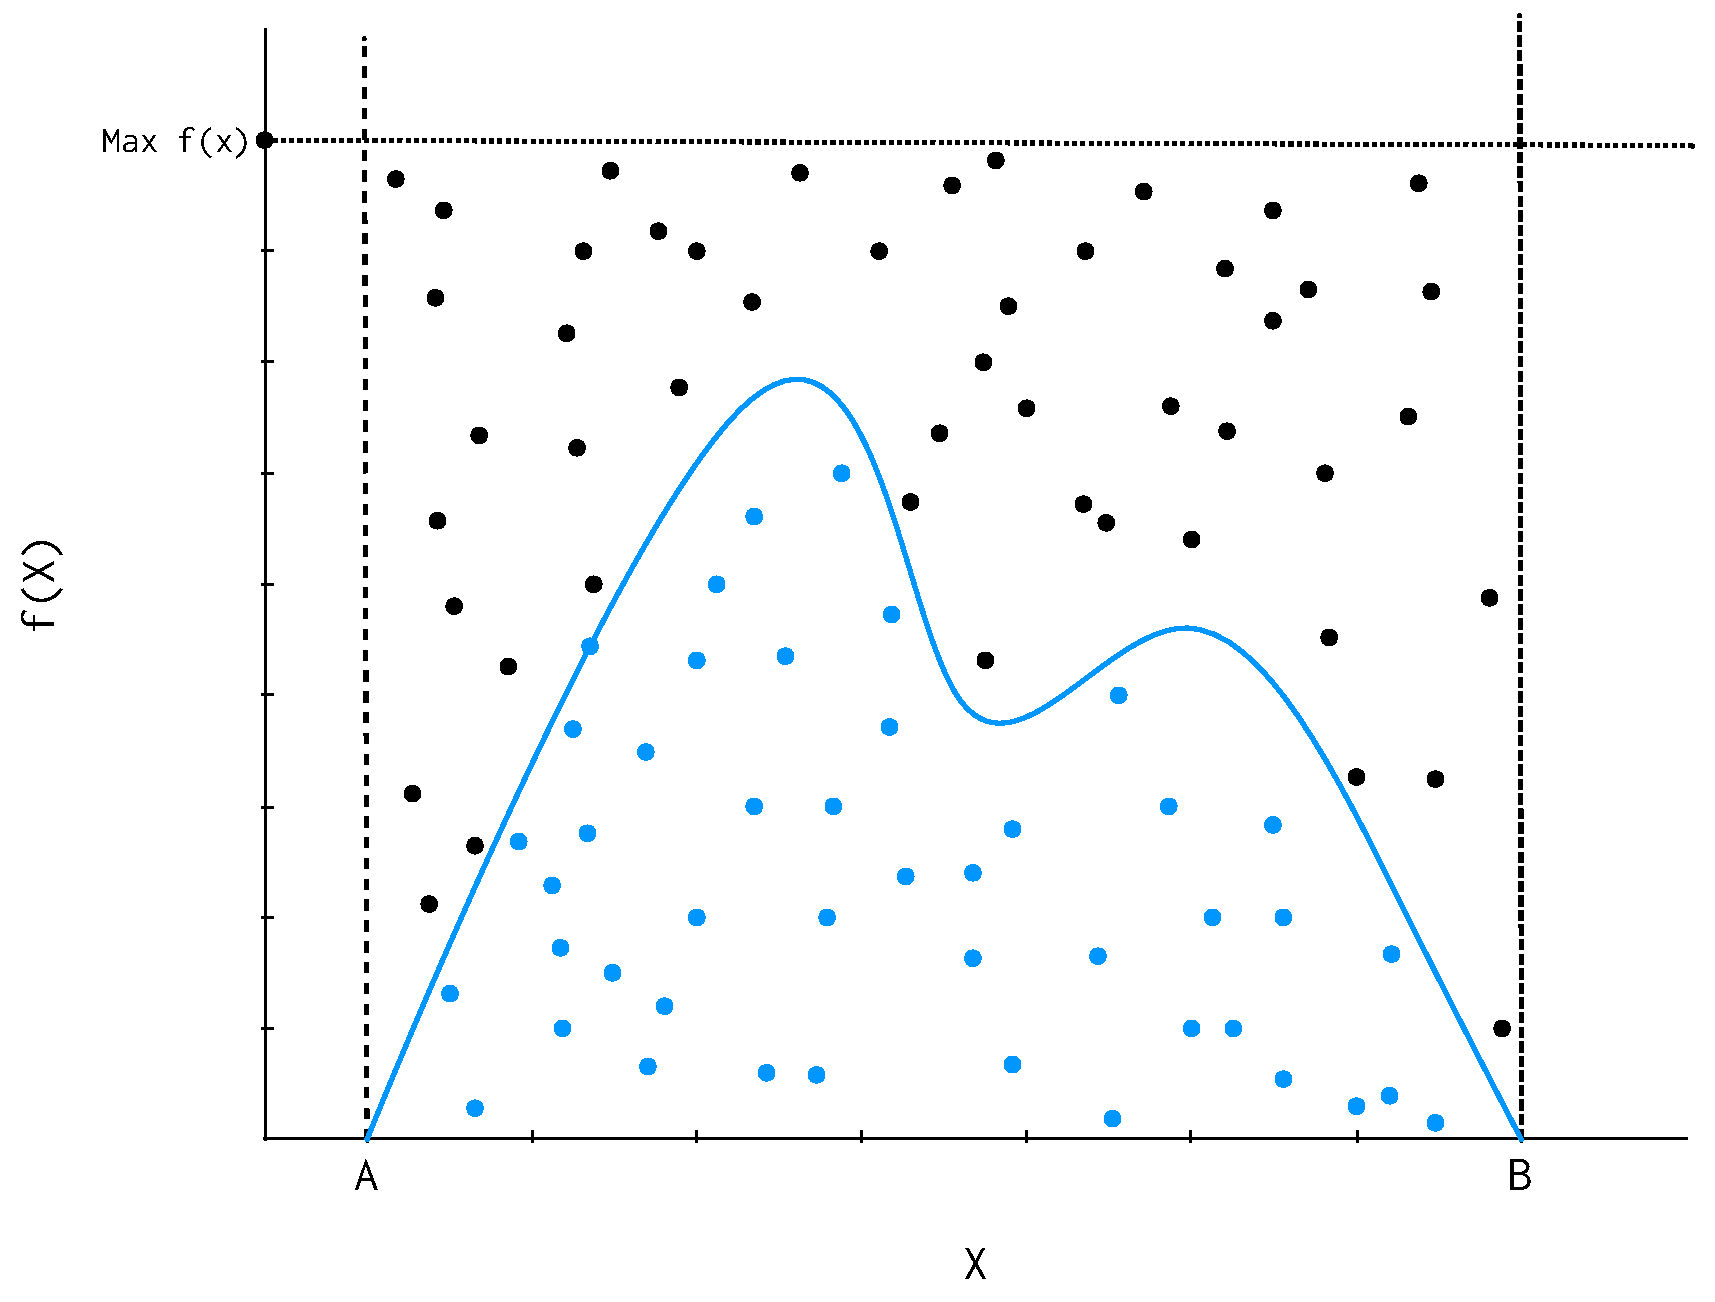
\includegraphics{reject.pdf}}
\caption{Rejection sampling of a bounded form. Area is estimated by the ratio of
accepted (open squares) to total points, multiplied by the rectangle
area.}\label{theory:bound}\end{figure}
\begin{gather}
\begin{split}\frac{\mbox{Points under curve}}{\mbox{Points generated}} \times \mbox{box area} = \lim_{n \to \infty} \int_A^B f(x) dx\end{split}\notag\\\begin{split}\end{split}\notag
\end{gather}
This approach is useful, for example, in estimating the normalizing constant for posterior distributions.
\begin{figure}[htbp]
\centering
\capstart

\scalebox{1.000000}{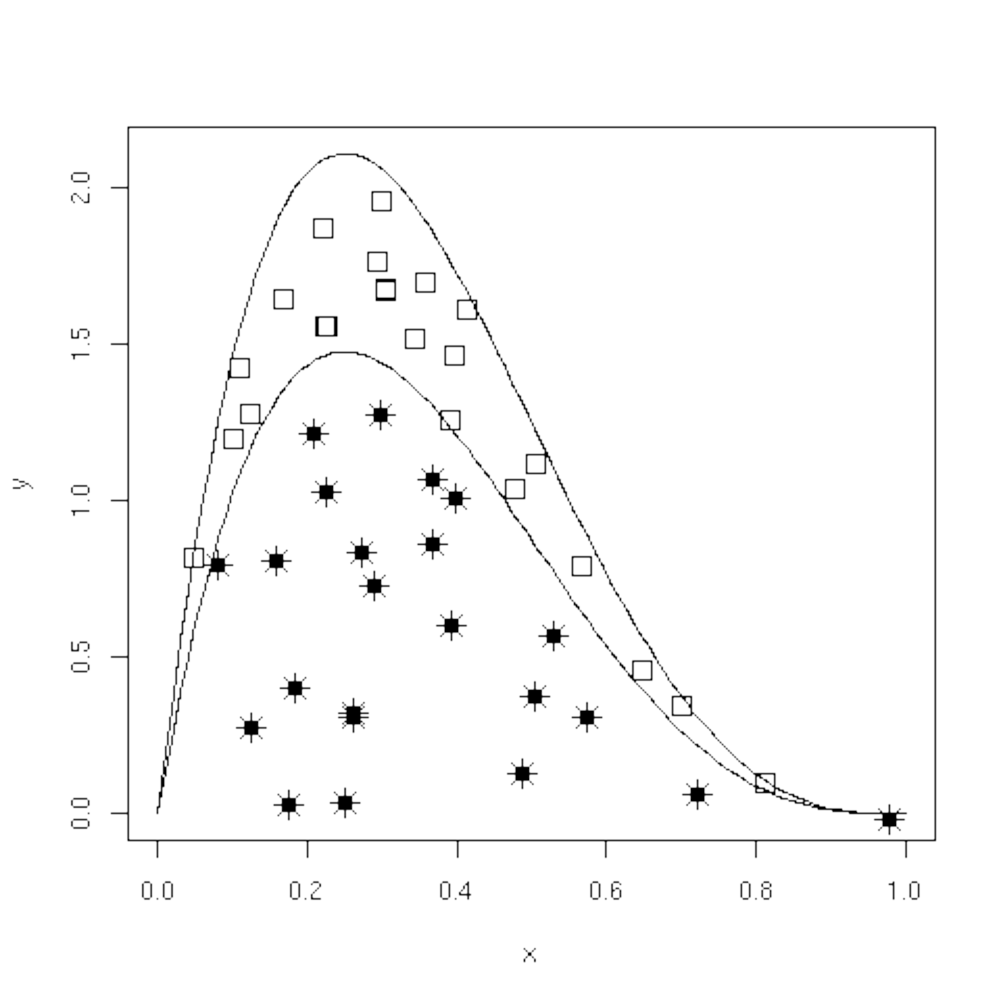
\includegraphics{envelope.pdf}}
\caption{Rejection sampling of an unbounded form using an enveloping distribution.}\label{theory:envelope}\end{figure}

If $f(x)$ has unbounded support (i.e. infinite tails), such as a Gaussian distribution, a bounding box is no longer appropriate. We must specify a majorizing (or, enveloping) function, $g(x)$, which implies:
\begin{gather}
\begin{split}g(x) \ge  f(x) \qquad\forall x \in (-\infty,\infty)\end{split}\notag\\\begin{split}\end{split}\notag
\end{gather}
Having done this, we can now sample ${x_i}$ from $g(x)$ and accept or reject each of these values based upon $f(x_i)$. Specifically, for each draw $x_i$, we also draw a uniform random variate $u_i$ and accept $x_i$ if $u_i < f(x_i)/cg(x_i)$, where $c$ is a constant (Figure {\hyperref[theory:envelope]{\emph{Rejection sampling of an unbounded form using an enveloping distribution.}}}). This approach is made more efficient by choosing an enveloping distribution that is ``close'' to the target distribution, thus maximizing the number of accepted points. Further improvement is gained by using optimized algorithms such as importance sampling which, as the name implies, samples more frequently from important areas of the distribution.

Rejection sampling is usually subject to declining performance as the dimension of the parameter space increases, so it is used less frequently than MCMC for evaluation of posterior distributions {\hyperref[references:gamerman-1997]{{[}Gamerman\_1997{]}}}.


\section{Markov Chains}
\label{theory:markov-chains}
A Markov chain is a special type of \emph{stochastic process}. The standard definition of a stochastic process is an ordered collection of random variables:
\begin{gather}
\begin{split}\{X_t:t \in T\}\end{split}\notag\\\begin{split}\end{split}\notag
\end{gather}
where $t$ is frequently (but not necessarily) a time index. If we think of $X_t$ as a state $X$ at time $t$, and invoke the following dependence condition on each state:
\begin{gather}
\begin{split}Pr(X_{t+1}=x_{t+1} | X_t=x_t, X_{t-1}=x_{t-1},\ldots,X_0=x_0) = Pr(X_{t+1}=x_{t+1} | X_t=x_t)\end{split}\notag\\\begin{split}\end{split}\notag
\end{gather}
then the stochastic process is known as a Markov chain. This conditioning specifies that the future depends on the current state, but not past states. Thus, the Markov chain wanders about the state space, remembering only where it has just been in the last time step. The collection of transition probabilities is sometimes called a \emph{transition matrix} when dealing with discrete states, or more generally, a \emph{transition kernel}.

In the context of Markov chain Monte Carlo, it is useful to think of the Markovian property as ``mild non-independence''. MCMC allows us to indirectly generate independent samples from a particular posterior distribution.


\subsection{Jargon-busting}
\label{theory:jargon-busting}
Before we move on, it is important to define some general properties of Markov chains. They are frequently encountered in the MCMC literature, and some will help us decide whether MCMC is producing a useful sample from the posterior.
\begin{itemize}
\item {} \begin{description}
\item[{\emph{Homogeneity}: A Markov chain is homogeneous at step $t$ if the}] \leavevmode
transition probabilities are independent of time $t$.

\end{description}

\item {} \begin{description}
\item[{\emph{Irreducibility}: A Markov chain is irreducible if every state is accessible}] \leavevmode
in one or more steps from any other state. That is, the chain contains no
absorbing states. This implies that there is a non-zero probability of
eventually reaching state $k$ from any other state in the chain.

\end{description}

\item {} \begin{description}
\item[{\emph{Recurrence}: States which are visited repeatedly are \emph{recurrent}. If the}] \leavevmode
expected time to return to a particular state is bounded, this is known as
\emph{positive recurrence}, otherwise the recurrent state is \emph{null recurrent}.
Further, a chain is \emph{Harris recurrent} when it visits all states $X
\in S$ infinitely often in the limit as $t \to \infty$; this is an
important characteristic when dealing with unbounded, continuous state
spaces. Whenever a chain ends up in a closed, irreducible set of Harris
recurrent states, it stays there forever and visits every state with
probability one.

\end{description}

\item {} \begin{description}
\item[{\emph{Stationarity}: A stationary Markov chain produces the same marginal}] \leavevmode\begin{quote}

distribution when multiplied by the transition kernel.  Thus, if $P$
is some $n \times n$ transition matrix:
\end{quote}
\begin{gather}
\begin{split}{\bf \pi P} = {\bf \pi}\end{split}\notag\\\begin{split}  for Markov chain :math:`\pi`. Thus, :math:`\pi` is no longer subscripted,
  and is referred to as the *limiting distribution* of the chain. In MCMC,
  the chain explores the state space according to its limiting marginal
  distribution.\end{split}\notag
\end{gather}
\end{description}

\item {} \begin{description}
\item[{\emph{Ergodicity}: Ergodicity is an emergent property of Markov chains which are}] \leavevmode
irreducible, positive Harris recurrent and aperiodic. Ergodicity is defined
as:

\end{description}
\begin{gather}
\begin{split}\lim_{n \to \infty} Pr^{(n)}(\theta_i \rightarrow \theta_j) = \pi(\theta) \quad \forall \theta_i, \theta_j \in \Theta\end{split}\notag\\\begin{split}  or in words, after many steps the marginal distribution of the chain is the
  same at one step as at all other steps. This implies that our Markov chain,
  which we recall is dependent, can generate samples that are independent if
  we wait long enough between samples. If it means anything to you,
  ergodicity is the analogue of the strong law of large numbers for Markov
  chains. For example, take values :math:`\theta_{i+1},\ldots,\theta_{i+n}`
  from a chain that has reached an ergodic state. A statistic of interest can
  then be estimated by:\end{split}\notag
\end{gather}\begin{gather}
\begin{split}\frac{1}{n}\sum_{j=i+1}^{i+n} h(\theta_j) \approx \int f(\theta) h(\theta) d\theta\end{split}\notag\\\begin{split}\end{split}\notag
\end{gather}
\end{itemize}


\section{Why MCMC Works: Reversible Markov Chains}
\label{theory:why-mcmc-works-reversible-markov-chains}
Markov chain Monte Carlo simulates a Markov chain for which some function of
interest (\emph{e.g.} the joint distribution of the parameters of some model) is the
unique, invariant limiting distribution. An invariant distribution with respect
to some Markov chain with transition kernel $Pr(y \mid x)$ implies that:
\begin{gather}
\begin{split}\int_x Pr(y \mid x) \pi(x) dx = \pi(y).\end{split}\notag\\\begin{split}\end{split}\notag
\end{gather}
Invariance is guaranteed for any \textbf{reversible} Markov chain. Consider a Markov
chain in reverse sequence:
$\{\theta^{(n)},\theta^{(n-1)},...,\theta^{(0)}\}$. This sequence is still
Markovian, because:
\begin{gather}
\begin{split}Pr(\theta^{(k)}=y \mid \theta^{(k+1)}=x,\theta^{(k+2)}=x_1,\ldots ) = Pr(\theta^{(k)}=y \mid \theta^{(k+1)}=x)\end{split}\notag\\\begin{split}\end{split}\notag
\end{gather}
Forward and reverse transition probabilities may be related through Bayes
theorem:
\begin{gather}
\begin{split}\end{split}\notag
\end{gather}\begin{gather}
\begin{split}\frac{Pr(\theta^{(k+1)}=x \mid \theta^{(k)}=y) \pi^{(k)}(y)}{\pi^{(k+1)}(x)}\end{split}\notag\\\begin{split}\end{split}\notag
\end{gather}
Though not homogeneous in general, $\pi$ becomes homogeneous if \textbf{Do you
ever call the stationary distribution itself homogeneous?}:
\begin{itemize}
\item {} 
$n \rightarrow \infty$

\item {} 
$\pi^{(i)}=\pi$ for some $i < k$

\end{itemize}

If this chain is homogeneous it is called reversible, because it satisfies the
\textbf{detailed balance equation}:
\begin{gather}
\begin{split}\pi(x)Pr(y \mid x) = \pi(y) Pr(x \mid y)\end{split}\notag\\\begin{split}\end{split}\notag
\end{gather}
Reversibility is important because it has the effect of balancing movement
through the entire state space. When a Markov chain is reversible, $\pi$
is the unique, invariant, stationary distribution of that chain. Hence, if
$\pi$ is of interest, we need only find the reversible Markov chain for
which $\pi$ is the limiting distribution. This is what MCMC does!


\section{Gibbs Sampling}
\label{theory:gibbs-sampling}
The Gibbs sampler is the simplest and most prevalent MCMC algorithm. If a
posterior has $k$ parameters to be estimated, we may condition each
parameter on current values of the other $k-1$ parameters, and sample from
the resultant distributional form (usually easier), and repeat this operation on
the other parameters in turn. This procedure generates samples from the
posterior distribution. Note that we have now combined Markov chains
(conditional independence) and Monte Carlo techniques (estimation by simulation)
to yield Markov chain Monte Carlo.

Here is a stereotypical Gibbs sampling algorithm:

As we can see from the algorithm, each distribution is conditioned on the last
iteration of its chain values, constituting a Markov chain as advertised. The
Gibbs sampler has all of the important properties outlined in the previous
section: it is aperiodic, homogeneous and ergodic. Once the sampler converges,
all subsequent samples are from the target distribution. This convergence occurs
at a geometric rate.
\begin{enumerate}
\item {} 
Choose starting values for states (parameters): ${\bf \theta} = [\theta_1^{(0)},\theta_2^{(0)},\ldots,\theta_k^{(0)}]$

\item {} 
Initialize counter $j=1$

\item {} 
Draw the following values from each of the $k$ conditional distributions:
\begin{eqnarray*}
\theta_1^{(j)} &\sim& \pi(\theta_1 | \theta_2^{(j-1)},\theta_3^{(j-1)},\ldots,\theta_{k-1}^{(j-1)},\theta_k^{(j-1)}) \\
\theta_2^{(j)} &\sim& \pi(\theta_2 | \theta_1^{(j)},\theta_3^{(j-1)},\ldots,\theta_{k-1}^{(j-1)},\theta_k^{(j-1)}) \\
\theta_3^{(j)} &\sim& \pi(\theta_3 | \theta_1^{(j)},\theta_2^{(j)},\ldots,\theta_{k-1}^{(j-1)},\theta_k^{(j-1)}) \\
\vdots \\
\theta_{k-1}^{(j)} &\sim& \pi(\theta_{k-1} | \theta_1^{(j)},\theta_2^{(j)},\ldots,\theta_{k-2}^{(j)},\theta_k^{(j-1)}) \\
\theta_k^{(j)} &\sim& \pi(\theta_k | \theta_1^{(j)},\theta_2^{(j)},\theta_4^{(j)},\ldots,\theta_{k-2}^{(j)},\theta_{k-1}^{(j)})
\end{eqnarray*}
\item {} 
Increment $j$ and repeat until convergence occurs.

\end{enumerate}


\section{The Metropolis-Hastings Algorithm}
\label{theory:the-metropolis-hastings-algorithm}
The key to success in applying the Gibbs sampler to the estimation of Bayesian
posteriors is being able to specify the form of the complete conditionals of
${\bf \theta}$. In fact, the algorithm cannot be implemented without them.
Of course, the posterior conditionals cannot always be neatly specified. In
contrast to the Gibbs algorithm, the Metropolis-Hastings algorithm generates
candidate state transitions from an alternate distribution, and accepts or
rejects each candidate probabilistically.

Let us first consider a simple Metropolis-Hastings algorithm for a single
parameter, $\theta$. We will use a standard sampling distribution,
referred to as the \emph{proposal distribution}, to produce candidate variables
$q_t(\theta^{\prime} | \theta)$. That is, the generated value,
$\theta^{\prime}$, is a \emph{possible} next value for $\theta$ at step
$t+1$. We also need to be able to calculate the probability of moving back
to the original value from the candidate, or
$q_t(\theta | \theta^{\prime})$. These probabilistic ingredients are used
to define an \emph{acceptance ratio}:
\begin{gather}
\begin{split}a(\theta^{\prime},\theta) = \frac{q_t(\theta^{\prime} | \theta) \pi(\theta^{\prime})}{q_t(\theta | \theta^{\prime}) \pi(\theta)}\end{split}\notag\\\begin{split}\end{split}\notag
\end{gather}
The value of $\theta^{(t+1)}$ is then determined by:
\begin{gather}
\begin{split}\theta^{(t+1)} = \left\{\begin{array}{l@{\quad \mbox{with prob.} \quad}l}\theta^{\prime} & \min(a(\theta^{\prime},\theta),1) \\ \theta^{(t)} & 1 - \min(a(\theta^{\prime},\theta),1) \end{array}\right.\end{split}\notag\\\begin{split}\end{split}\notag
\end{gather}
This transition kernel implies that movement is not guaranteed at every step. It
only occurs if the suggested transition is likely based on the acceptance ratio.

A single iteration of the Metropolis-Hastings algorithm proceeds as follows:

The original form of the algorithm specified by Metropolis required that
$q_t(\theta^{\prime} | \theta) = q_t(\theta | \theta^{\prime})$, which
reduces $a(\theta^{\prime},\theta)$ to
$\pi(\theta^{\prime})/\pi(\theta)$, but this is not necessary. In either
case, the state moves to high-density points in the distribution with high
probability, and to low-density points with low probability. After convergence,
the Metropolis-Hastings algorithm describes the full target posterior density,
so all points are recurrent.
\begin{enumerate}
\item {} 
Sample $\theta^{\prime}$ from $q(\theta^{\prime} | \theta^{(t)})$.

\item {} 
Generate a Uniform{[}0,1{]} random variate $u$.

\item {} 
If $a(\theta^{\prime},\theta) > u$ then $\theta^{(t+1)} = \theta^{\prime}$, otherwise $\theta^{(t+1)} = \theta^{(t)}$.

\end{enumerate}


\subsection{Random-walk Metropolis-Hastings}
\label{theory:random-walk-metropolis-hastings}
A practical implementation of the Metropolis-Hastings algorithm makes use of a
random-walk proposal. Recall that a random walk is a Markov chain that evolves
according to:
\begin{eqnarray*}
\theta^{(t+1)} &=& \theta^{(t)} + \epsilon_t \\
\epsilon_t &\sim& f(\phi)
\end{eqnarray*}
As applied to the MCMC sampling, the random walk is used as a proposal
distribution, whereby dependent proposals are generated according to:
\begin{gather}
\begin{split}q(\theta^{\prime} | \theta^{(t)}) = f(\theta^{\prime} - \theta^{(t)}) = \theta^{(t)} + \epsilon_t\end{split}\notag\\\begin{split}\end{split}\notag
\end{gather}
Generally, the density generating $\epsilon_t$ is symmetric about zero,
resulting in a symmetric chain. Chain symmetry implies that
$q(\theta^{\prime} | \theta^{(t)}) = q(\theta^{(t)} | \theta^{\prime})$,
which reduces the Metropolis-Hastings acceptance ratio to:
\begin{gather}
\begin{split}a(\theta^{\prime},\theta) = \frac{\pi(\theta^{\prime})}{\pi(\theta)}\end{split}\notag\\\begin{split}\end{split}\notag
\end{gather}
The choice of the random walk distribution for $\epsilon_t$ is frequently
a normal or Student's $t$ density, but it may be any distribution that
generates an irreducible proposal chain.

An important consideration is the specification of the scale parameter for the
random walk error distribution. Large values produce random walk steps that are
highly exploratory, but tend to produce proposal values in the tails of the
target distribution, potentially resulting in very small acceptance rates.
Conversely, small values tend to be accepted more frequently, since they tend to
produce proposals close to the current parameter value, but may result in chains
that mix very slowly. Some simulation studies suggest optimal acceptance rates
in the range of 20-50\%. It is often worthwhile to optimize the proposal variance
by iteratively adjusting its value, according to observed acceptance rates early
in the MCMC simulation {\hyperref[references:gamerman-1997]{{[}Gamerman\_1997{]}}}.


\chapter{List of References}
\label{references:list-of-references}\label{references::doc}

\chapter{Indices and tables}
\label{index:indices-and-tables}\begin{itemize}
\item {} 
\emph{genindex}

\item {} 
\emph{modindex}

\item {} 
\emph{search}

\end{itemize}

\begin{thebibliography}{Christakos_2002}
\bibitem[Akaike_1973]{Akaike_1973}{\phantomsection\label{references:akaike_1973} \begin{enumerate}
\setcounter{enumi}{7}
\item {} 
Akaike. Information theory as an extension of the maximum likelihood principle. In B.N. Petrov and F. Csaki, editors, Second International Symposium on Information Theory, pages 267–281, Akademiai Kiado, Budapest, 1973.

\end{enumerate}
}
\bibitem[Bernardo_1992]{Bernardo_1992}{\phantomsection\label{references:bernardo_1992} 
J.M. Bernardo, J. Berger, A.P. Dawid, and J.F.M. Smith, editors. Bayesian Statistics 4. Oxford University Press, Oxford, 1992.
}
\bibitem[Brooks_2000]{Brooks_2000}{\phantomsection\label{references:brooks_2000} 
S.P. Brooks, E.A. Catchpole, and B.J.T. Morgan. Bayesian animal survival estimation. Statistical Science, 15: 357–376, 2000.
}
\bibitem[Burnham_2002]{Burnham_2002}{\phantomsection\label{references:burnham_2002} 
K.P. Burnham and D.R. Anderson. Model Selection and Multi-Model Inference: A Practical, Information-theoretic Approach. Springer, New York, 2002.
}
\bibitem[Christakos_2002]{Christakos_2002}{\phantomsection\label{references:christakos_2002} \begin{enumerate}
\setcounter{enumi}{6}
\item {} 
Christakos. On the assimilation of uncertain physical knowledge bases: Bayesian and non-Bayesian techniques. Advances in Water Resources, 2002.

\end{enumerate}
}
\bibitem[Gamerman_1997]{Gamerman_1997}{\phantomsection\label{references:gamerman_1997} \begin{enumerate}
\setcounter{enumi}{3}
\item {} 
Gamerman. Markov Chain Monte Carlo: statistical simulation for Bayesian inference. Chapman and Hall, 1997.

\end{enumerate}
}
\bibitem[Gelman_1996]{Gelman_1996}{\phantomsection\label{references:gelman_1996} \begin{enumerate}
\item {} 
Gelman, X.L. Meng, and H. Stern. Posterior predictive assessment of model fitness via realized discrepencies with discussion. Statistica Sinica, 6, 1996.

\end{enumerate}
}
\bibitem[Gelman_2004]{Gelman_2004}{\phantomsection\label{references:gelman_2004} \begin{enumerate}
\item {} 
Gelman, J.B. Carlin, H.S. Stern, and D.B. Rubin. Bayesian Data Analysis, Second Edition. Chapman and Hall/CRC, Boca Raton, FL, 2004.

\end{enumerate}
}
\bibitem[Geweke_1992]{Geweke_1992}{\phantomsection\label{references:geweke_1992} \begin{enumerate}
\setcounter{enumi}{9}
\item {} 
Geweke. Evaluating the accuracy of sampling-based approaches to calculating posterior moments. In Bernardo et al. {[}1992{]}, pages 169–193.

\end{enumerate}
}
\bibitem[Haario_2001]{Haario_2001}{\phantomsection\label{references:haario_2001} \begin{enumerate}
\setcounter{enumi}{7}
\item {} 
Haario, E. Saksman, and J. Tamminen. An adaptive metropolis algorithm. Bernoulli, 7(2):223–242, 2001.

\end{enumerate}
}
\bibitem[Jarrett_1979]{Jarrett_1979}{\phantomsection\label{references:jarrett_1979} 
R.G. Jarrett. A note on the intervals between coal mining disasters. Biometrika, 66:191–193, 1979.
}
\bibitem[Jaynes_2003]{Jaynes_2003}{\phantomsection\label{references:jaynes_2003} 
E.T. Jaynes. Probability theory: the logic of science. Cambridge university press, 2003.
}
\bibitem[Jordan_2004]{Jordan_2004}{\phantomsection\label{references:jordan_2004} 
M.I. Jordan. Graphical models. Statist. Sci., 19(1):140–155, 2004.
}
\bibitem[Kerman_2004]{Kerman_2004}{\phantomsection\label{references:kerman_2004} \begin{enumerate}
\setcounter{enumi}{9}
\item {} 
Kerman and A. Gelman. Fully Bayesian computing. Available at SSRN: \href{http://ssrn.com/abstract=1010387}{http://ssrn.com/abstract=1010387}, 2004.

\end{enumerate}
}
\bibitem[Langtangen_2009]{Langtangen_2009}{\phantomsection\label{references:langtangen_2009} 
Hans Petter Langtangen. Python Scripting for Computational Science. Springer-Verlag, 2009.
}
\bibitem[Lauritzen_1990]{Lauritzen_1990}{\phantomsection\label{references:lauritzen_1990} 
S.L. Lauritzen, A.P. Dawid, B.N. Larsen, and H.G. Leimer. Independence properties of directed Markov fields. Networks, 20:491–505, 1990.
}
\bibitem[Lutz_2007]{Lutz_2007}{\phantomsection\label{references:lutz_2007} \begin{enumerate}
\setcounter{enumi}{12}
\item {} 
Lutz. Learning Python. O’Reilly, 2007.

\end{enumerate}
}
\bibitem[Oberhumer_2008]{Oberhumer_2008}{\phantomsection\label{references:oberhumer_2008} 
M.F.X.J. Oberhumer. LZO Real-Time Data Compression Library. 2008. URL \href{http://www.oberhumer.com/opensource/lzo/}{http://www.oberhumer.com/opensource/lzo/}.
}
\bibitem[Plummer_2008]{Plummer_2008}{\phantomsection\label{references:plummer_2008} \begin{enumerate}
\setcounter{enumi}{12}
\item {} 
Plummer, N. Best, K. Cowles and K. Vines. coda: Output Analysis and Diagnostics for MCMC. R package version 0.13-3, 2008. URL \href{http://CRAN.R-project.org/package=coda}{http://CRAN.R-project.org/package=coda}.

\end{enumerate}
}
\bibitem[R_2010]{R_2010}{\phantomsection\label{references:r_2010} 
R Development Core Team. R: A Language and Environment for Statistical Computing. R Foundation for Statistical Computing, Vienna, Austria. ISBN 3-900051-07-0, 2010. URL http: //www.R-project.org/.
}
\bibitem[Raftery_1995a]{Raftery_1995a}{\phantomsection\label{references:raftery_1995a} 
A.E. Raftery and S.M. Lewis. The number of iterations, convergence diagnostics and generic metropolis al- gorithms. In D.J. Spiegelhalter W.R. Gilks and S. Richardson, editors, Practical Markov Chain Monte Carlo. Chapman and Hall, London, U.K., 1995.
}
\bibitem[Raftery_1995b]{Raftery_1995b}{\phantomsection\label{references:raftery_1995b} 
A.E. Raftery and S.M. Lewis. Gibbsit Version 2.0. 1995. URL \href{http://lib.stat.cmu.edu/}{http://lib.stat.cmu.edu/} general/gibbsit/.
}
\bibitem[Roelofs_2010]{Roelofs_2010}{\phantomsection\label{references:roelofs_2010} \begin{enumerate}
\setcounter{enumi}{6}
\item {} 
Roelofs, J. loup Gailly, M. Adler. zlib: A Massively Spiffy Yet Delicately Unobtrusive Compression Library. 2010. URL \href{http://www.zlib.net/}{http://www.zlib.net/}.

\end{enumerate}
}
\bibitem[Roberts_2007]{Roberts_2007}{\phantomsection\label{references:roberts_2007} 
G.O. Roberts and J.S. Rosenthal. Implementing componentwise Hastings algorithms. Journal of Applied Probability, 44(2):458–475, 2007.
}
\bibitem[Schwarz_1978]{Schwarz_1978}{\phantomsection\label{references:schwarz_1978} \begin{enumerate}
\setcounter{enumi}{6}
\item {} 
Schwarz. Estimating the dimension of a model. The Annals of Statistics, 6(2):461–464, 1978.

\end{enumerate}
}
\bibitem[Seward_2007]{Seward_2007}{\phantomsection\label{references:seward_2007} \begin{enumerate}
\setcounter{enumi}{9}
\item {} 
Seward. bzip2 and libbzip2, Version 1.0.5 – A Program and Library for Data Compression. 2007. URL \href{http://www.bzip.org/}{http://www.bzip.org/}.

\end{enumerate}
}
\bibitem[vanRossum_2010]{vanRossum_2010}{\phantomsection\label{references:vanrossum_2010} \begin{enumerate}
\setcounter{enumi}{6}
\item {} 
van Rossum. The Python Library Reference Release 2.6.5., 2010. URL \href{http://docs}{http://docs}. python.org/library/.

\end{enumerate}
}
\end{thebibliography}


\renewcommand{\indexname}{Python Module Index}
\begin{theindex}
\def\bigletter#1{{\Large\sffamily#1}\nopagebreak\vspace{1mm}}
\bigletter{p}
\item {\texttt{pymc.distributions}}, \pageref{distributions:module-pymc.distributions}
\end{theindex}

\renewcommand{\indexname}{Index}
\printindex
\end{document}

\chapter{epydoc class reference?}

\chapter{Database backends}
David
Link to the epydoc generated API ?

\end{document}
 
